\documentclass[twoside]{book}

% Packages required by doxygen
\usepackage{fixltx2e}
\usepackage{calc}
\usepackage{doxygen}
\usepackage[export]{adjustbox} % also loads graphicx
\usepackage{graphicx}
\usepackage[utf8]{inputenc}
\usepackage{makeidx}
\usepackage{multicol}
\usepackage{multirow}
\PassOptionsToPackage{warn}{textcomp}
\usepackage{textcomp}
\usepackage[nointegrals]{wasysym}
\usepackage[table]{xcolor}

% Font selection
\usepackage[T1]{fontenc}
\usepackage[scaled=.90]{helvet}
\usepackage{courier}
\usepackage{amssymb}
\usepackage{sectsty}
\renewcommand{\familydefault}{\sfdefault}
\allsectionsfont{%
  \fontseries{bc}\selectfont%
  \color{darkgray}%
}
\renewcommand{\DoxyLabelFont}{%
  \fontseries{bc}\selectfont%
  \color{darkgray}%
}
\newcommand{\+}{\discretionary{\mbox{\scriptsize$\hookleftarrow$}}{}{}}

% Page & text layout
\usepackage{geometry}
\geometry{%
  a4paper,%
  top=2.5cm,%
  bottom=2.5cm,%
  left=2.5cm,%
  right=2.5cm%
}
\tolerance=750
\hfuzz=15pt
\hbadness=750
\setlength{\emergencystretch}{15pt}
\setlength{\parindent}{0cm}
\setlength{\parskip}{3ex plus 2ex minus 2ex}
\makeatletter
\renewcommand{\paragraph}{%
  \@startsection{paragraph}{4}{0ex}{-1.0ex}{1.0ex}{%
    \normalfont\normalsize\bfseries\SS@parafont%
  }%
}
\renewcommand{\subparagraph}{%
  \@startsection{subparagraph}{5}{0ex}{-1.0ex}{1.0ex}{%
    \normalfont\normalsize\bfseries\SS@subparafont%
  }%
}
\makeatother

% Headers & footers
\usepackage{fancyhdr}
\pagestyle{fancyplain}
\fancyhead[LE]{\fancyplain{}{\bfseries\thepage}}
\fancyhead[CE]{\fancyplain{}{}}
\fancyhead[RE]{\fancyplain{}{\bfseries\leftmark}}
\fancyhead[LO]{\fancyplain{}{\bfseries\rightmark}}
\fancyhead[CO]{\fancyplain{}{}}
\fancyhead[RO]{\fancyplain{}{\bfseries\thepage}}
\fancyfoot[LE]{\fancyplain{}{}}
\fancyfoot[CE]{\fancyplain{}{}}
\fancyfoot[RE]{\fancyplain{}{\bfseries\scriptsize Generated by Doxygen }}
\fancyfoot[LO]{\fancyplain{}{\bfseries\scriptsize Generated by Doxygen }}
\fancyfoot[CO]{\fancyplain{}{}}
\fancyfoot[RO]{\fancyplain{}{}}
\renewcommand{\footrulewidth}{0.4pt}
\renewcommand{\chaptermark}[1]{%
  \markboth{#1}{}%
}
\renewcommand{\sectionmark}[1]{%
  \markright{\thesection\ #1}%
}

% Indices & bibliography
\usepackage{natbib}
\usepackage[titles]{tocloft}
\setcounter{tocdepth}{3}
\setcounter{secnumdepth}{5}
\makeindex

% Hyperlinks (required, but should be loaded last)
\usepackage{ifpdf}
\ifpdf
  \usepackage[pdftex,pagebackref=true]{hyperref}
\else
  \usepackage[ps2pdf,pagebackref=true]{hyperref}
\fi
\hypersetup{%
  colorlinks=true,%
  linkcolor=blue,%
  citecolor=blue,%
  unicode%
}

% Custom commands
\newcommand{\clearemptydoublepage}{%
  \newpage{\pagestyle{empty}\cleardoublepage}%
}

\usepackage{caption}
\captionsetup{labelsep=space,justification=centering,font={bf},singlelinecheck=off,skip=4pt,position=top}

%===== C O N T E N T S =====

\begin{document}

% Titlepage & ToC
\hypersetup{pageanchor=false,
             bookmarksnumbered=true,
             pdfencoding=unicode
            }
\pagenumbering{alph}
\begin{titlepage}
\vspace*{7cm}
\begin{center}%
{\Large Train\+Vagas \\[1ex]\large 0.\+1 }\\
\vspace*{1cm}
{\large Generated by Doxygen 1.8.13}\\
\end{center}
\end{titlepage}
\clearemptydoublepage
\pagenumbering{roman}
\tableofcontents
\clearemptydoublepage
\pagenumbering{arabic}
\hypersetup{pageanchor=true}

%--- Begin generated contents ---
\chapter{Namespace Index}
\section{Packages}
Here are the packages with brief descriptions (if available)\+:\begin{DoxyCompactList}
\item\contentsline{section}{\hyperlink{namespacecontroller}{controller} }{\pageref{namespacecontroller}}{}
\item\contentsline{section}{\hyperlink{namespacedomain}{domain} }{\pageref{namespacedomain}}{}
\item\contentsline{section}{\hyperlink{namespacefrontend}{frontend} }{\pageref{namespacefrontend}}{}
\item\contentsline{section}{\hyperlink{namespacesoftware}{software} }{\pageref{namespacesoftware}}{}
\item\contentsline{section}{\hyperlink{namespacetest}{test} }{\pageref{namespacetest}}{}
\item\contentsline{section}{\hyperlink{namespacetranslate}{translate} }{\pageref{namespacetranslate}}{}
\item\contentsline{section}{\hyperlink{namespaceutilities}{utilities} }{\pageref{namespaceutilities}}{}
\end{DoxyCompactList}

\chapter{Hierarchical Index}
\section{Class Hierarchy}
This inheritance list is sorted roughly, but not completely, alphabetically\+:\begin{DoxyCompactList}
\item \contentsline{section}{domain.\+Calculate\+Distance}{\pageref{classdomain_1_1_calculate_distance}}{}
\item \contentsline{section}{test.\+Calculate\+Distance\+Test}{\pageref{classtest_1_1_calculate_distance_test}}{}
\item \contentsline{section}{utilities.\+Data\+File}{\pageref{classutilities_1_1_data_file}}{}
\item \contentsline{section}{test.\+Data\+File\+Test}{\pageref{classtest_1_1_data_file_test}}{}
\item \contentsline{section}{frontend.\+Display}{\pageref{classfrontend_1_1_display}}{}
\item \contentsline{section}{utilities.\+File\+Property}{\pageref{enumutilities_1_1_file_property}}{}
\item \contentsline{section}{domain.\+Filter}{\pageref{classdomain_1_1_filter}}{}
\item \contentsline{section}{test.\+Filter\+Test}{\pageref{classtest_1_1_filter_test}}{}
\item \contentsline{section}{domain.\+Graph}{\pageref{classdomain_1_1_graph}}{}
\item \contentsline{section}{test.\+Graph\+Test}{\pageref{classtest_1_1_graph_test}}{}
\item \contentsline{section}{software.\+main}{\pageref{classsoftware_1_1main}}{}
\item \contentsline{section}{utilities.\+Permutation}{\pageref{classutilities_1_1_permutation}}{}
\item \contentsline{section}{test.\+Permutation\+Test}{\pageref{classtest_1_1_permutation_test}}{}
\item \contentsline{section}{controller.\+Rail\+System}{\pageref{classcontroller_1_1_rail_system}}{}
\item \contentsline{section}{test.\+Rail\+System\+Test}{\pageref{classtest_1_1_rail_system_test}}{}
\item \contentsline{section}{domain.\+Route}{\pageref{classdomain_1_1_route}}{}
\item \contentsline{section}{test.\+Route\+Test}{\pageref{classtest_1_1_route_test}}{}
\item \contentsline{section}{domain.\+Shortest\+Route}{\pageref{classdomain_1_1_shortest_route}}{}
\item \contentsline{section}{test.\+Shortest\+Route\+Test}{\pageref{classtest_1_1_shortest_route_test}}{}
\item \contentsline{section}{domain.\+Town}{\pageref{classdomain_1_1_town}}{}
\item \contentsline{section}{test.\+Town\+Test}{\pageref{classtest_1_1_town_test}}{}
\item \contentsline{section}{translate.\+Translate}{\pageref{classtranslate_1_1_translate}}{}
\item \contentsline{section}{translate.\+Translate\+Message}{\pageref{interfacetranslate_1_1_translate_message}}{}
\begin{DoxyCompactList}
\item \contentsline{section}{translate.\+Pt\+BR}{\pageref{classtranslate_1_1_pt_b_r}}{}
\end{DoxyCompactList}
\end{DoxyCompactList}

\chapter{Class Index}
\section{Class List}
Here are the classes, structs, unions and interfaces with brief descriptions\+:\begin{DoxyCompactList}
\item\contentsline{section}{\hyperlink{classdomain_1_1_calculate_distance}{domain.\+Calculate\+Distance} }{\pageref{classdomain_1_1_calculate_distance}}{}
\item\contentsline{section}{\hyperlink{classtest_1_1_calculate_distance_test}{test.\+Calculate\+Distance\+Test} }{\pageref{classtest_1_1_calculate_distance_test}}{}
\item\contentsline{section}{\hyperlink{classutilities_1_1_data_file}{utilities.\+Data\+File} }{\pageref{classutilities_1_1_data_file}}{}
\item\contentsline{section}{\hyperlink{classtest_1_1_data_file_test}{test.\+Data\+File\+Test} }{\pageref{classtest_1_1_data_file_test}}{}
\item\contentsline{section}{\hyperlink{classfrontend_1_1_display}{frontend.\+Display} }{\pageref{classfrontend_1_1_display}}{}
\item\contentsline{section}{\hyperlink{enumutilities_1_1_file_property}{utilities.\+File\+Property} }{\pageref{enumutilities_1_1_file_property}}{}
\item\contentsline{section}{\hyperlink{classdomain_1_1_filter}{domain.\+Filter} }{\pageref{classdomain_1_1_filter}}{}
\item\contentsline{section}{\hyperlink{classtest_1_1_filter_test}{test.\+Filter\+Test} }{\pageref{classtest_1_1_filter_test}}{}
\item\contentsline{section}{\hyperlink{classdomain_1_1_graph}{domain.\+Graph} }{\pageref{classdomain_1_1_graph}}{}
\item\contentsline{section}{\hyperlink{classtest_1_1_graph_test}{test.\+Graph\+Test} }{\pageref{classtest_1_1_graph_test}}{}
\item\contentsline{section}{\hyperlink{classsoftware_1_1main}{software.\+main} }{\pageref{classsoftware_1_1main}}{}
\item\contentsline{section}{\hyperlink{classutilities_1_1_permutation}{utilities.\+Permutation} }{\pageref{classutilities_1_1_permutation}}{}
\item\contentsline{section}{\hyperlink{classtest_1_1_permutation_test}{test.\+Permutation\+Test} }{\pageref{classtest_1_1_permutation_test}}{}
\item\contentsline{section}{\hyperlink{classtranslate_1_1_pt_b_r}{translate.\+Pt\+BR} }{\pageref{classtranslate_1_1_pt_b_r}}{}
\item\contentsline{section}{\hyperlink{classcontroller_1_1_rail_system}{controller.\+Rail\+System} }{\pageref{classcontroller_1_1_rail_system}}{}
\item\contentsline{section}{\hyperlink{classtest_1_1_rail_system_test}{test.\+Rail\+System\+Test} }{\pageref{classtest_1_1_rail_system_test}}{}
\item\contentsline{section}{\hyperlink{classdomain_1_1_route}{domain.\+Route} }{\pageref{classdomain_1_1_route}}{}
\item\contentsline{section}{\hyperlink{classtest_1_1_route_test}{test.\+Route\+Test} }{\pageref{classtest_1_1_route_test}}{}
\item\contentsline{section}{\hyperlink{classdomain_1_1_shortest_route}{domain.\+Shortest\+Route} }{\pageref{classdomain_1_1_shortest_route}}{}
\item\contentsline{section}{\hyperlink{classtest_1_1_shortest_route_test}{test.\+Shortest\+Route\+Test} }{\pageref{classtest_1_1_shortest_route_test}}{}
\item\contentsline{section}{\hyperlink{classdomain_1_1_town}{domain.\+Town} }{\pageref{classdomain_1_1_town}}{}
\item\contentsline{section}{\hyperlink{classtest_1_1_town_test}{test.\+Town\+Test} }{\pageref{classtest_1_1_town_test}}{}
\item\contentsline{section}{\hyperlink{classtranslate_1_1_translate}{translate.\+Translate} }{\pageref{classtranslate_1_1_translate}}{}
\item\contentsline{section}{\hyperlink{interfacetranslate_1_1_translate_message}{translate.\+Translate\+Message} }{\pageref{interfacetranslate_1_1_translate_message}}{}
\end{DoxyCompactList}

\chapter{File Index}
\section{File List}
Here is a list of all files with brief descriptions\+:\begin{DoxyCompactList}
\item\contentsline{section}{D\+:/workspace/\+Train\+Vagas/src/controller/\hyperlink{_rail_system_8java}{Rail\+System.\+java} \\*Software de gerenciamento das rotas para uma solucao de mobilidade sobre trilhos }{\pageref{_rail_system_8java}}{}
\item\contentsline{section}{D\+:/workspace/\+Train\+Vagas/src/domain/\hyperlink{_calculate_distance_8java}{Calculate\+Distance.\+java} \\*Software de gerenciamento das rotas para uma solucao de mobilidade sobre trilhos }{\pageref{_calculate_distance_8java}}{}
\item\contentsline{section}{D\+:/workspace/\+Train\+Vagas/src/domain/\hyperlink{_filter_8java}{Filter.\+java} \\*Software de gerenciamento das rotas para uma solucao de mobilidade sobre trilhos }{\pageref{_filter_8java}}{}
\item\contentsline{section}{D\+:/workspace/\+Train\+Vagas/src/domain/\hyperlink{_graph_8java}{Graph.\+java} \\*Software de gerenciamento das rotas para uma solucao de mobilidade sobre trilhos }{\pageref{_graph_8java}}{}
\item\contentsline{section}{D\+:/workspace/\+Train\+Vagas/src/domain/\hyperlink{_route_8java}{Route.\+java} \\*Software de gerenciamento das rotas para uma solucao de mobilidade sobre trilhos }{\pageref{_route_8java}}{}
\item\contentsline{section}{D\+:/workspace/\+Train\+Vagas/src/domain/\hyperlink{_shortest_route_8java}{Shortest\+Route.\+java} \\*Software de gerenciamento das rotas para uma solucao de mobilidade sobre trilhos }{\pageref{_shortest_route_8java}}{}
\item\contentsline{section}{D\+:/workspace/\+Train\+Vagas/src/domain/\hyperlink{_town_8java}{Town.\+java} \\*Software de gerenciamento das rotas para uma solucao de mobilidade sobre trilhos }{\pageref{_town_8java}}{}
\item\contentsline{section}{D\+:/workspace/\+Train\+Vagas/src/frontend/\hyperlink{_display_8java}{Display.\+java} \\*Software de gerenciamento das rotas para uma solucao de mobilidade sobre trilhos }{\pageref{_display_8java}}{}
\item\contentsline{section}{D\+:/workspace/\+Train\+Vagas/src/software/\hyperlink{main_8java}{main.\+java} \\*Software de gerenciamento das rotas para uma solucao de mobilidade sobre trilhos }{\pageref{main_8java}}{}
\item\contentsline{section}{D\+:/workspace/\+Train\+Vagas/src/test/\hyperlink{_calculate_distance_test_8java}{Calculate\+Distance\+Test.\+java} }{\pageref{_calculate_distance_test_8java}}{}
\item\contentsline{section}{D\+:/workspace/\+Train\+Vagas/src/test/\hyperlink{_data_file_test_8java}{Data\+File\+Test.\+java} }{\pageref{_data_file_test_8java}}{}
\item\contentsline{section}{D\+:/workspace/\+Train\+Vagas/src/test/\hyperlink{_filter_test_8java}{Filter\+Test.\+java} }{\pageref{_filter_test_8java}}{}
\item\contentsline{section}{D\+:/workspace/\+Train\+Vagas/src/test/\hyperlink{_graph_test_8java}{Graph\+Test.\+java} }{\pageref{_graph_test_8java}}{}
\item\contentsline{section}{D\+:/workspace/\+Train\+Vagas/src/test/\hyperlink{_permutation_test_8java}{Permutation\+Test.\+java} }{\pageref{_permutation_test_8java}}{}
\item\contentsline{section}{D\+:/workspace/\+Train\+Vagas/src/test/\hyperlink{_rail_system_test_8java}{Rail\+System\+Test.\+java} }{\pageref{_rail_system_test_8java}}{}
\item\contentsline{section}{D\+:/workspace/\+Train\+Vagas/src/test/\hyperlink{_route_test_8java}{Route\+Test.\+java} }{\pageref{_route_test_8java}}{}
\item\contentsline{section}{D\+:/workspace/\+Train\+Vagas/src/test/\hyperlink{_shortest_route_test_8java}{Shortest\+Route\+Test.\+java} }{\pageref{_shortest_route_test_8java}}{}
\item\contentsline{section}{D\+:/workspace/\+Train\+Vagas/src/test/\hyperlink{_town_test_8java}{Town\+Test.\+java} }{\pageref{_town_test_8java}}{}
\item\contentsline{section}{D\+:/workspace/\+Train\+Vagas/src/translate/\hyperlink{_pt_b_r_8java}{Pt\+B\+R.\+java} \\*Software de gerenciamento das rotas para uma solucao de mobilidade sobre trilhos }{\pageref{_pt_b_r_8java}}{}
\item\contentsline{section}{D\+:/workspace/\+Train\+Vagas/src/translate/\hyperlink{_translate_8java}{Translate.\+java} }{\pageref{_translate_8java}}{}
\item\contentsline{section}{D\+:/workspace/\+Train\+Vagas/src/translate/\hyperlink{_translate_message_8java}{Translate\+Message.\+java} \\*Software de gerenciamento das rotas para uma solucao de mobilidade sobre trilhos }{\pageref{_translate_message_8java}}{}
\item\contentsline{section}{D\+:/workspace/\+Train\+Vagas/src/utilities/\hyperlink{_data_file_8java}{Data\+File.\+java} }{\pageref{_data_file_8java}}{}
\item\contentsline{section}{D\+:/workspace/\+Train\+Vagas/src/utilities/\hyperlink{_file_property_8java}{File\+Property.\+java} }{\pageref{_file_property_8java}}{}
\item\contentsline{section}{D\+:/workspace/\+Train\+Vagas/src/utilities/\hyperlink{_permutation_8java}{Permutation.\+java} }{\pageref{_permutation_8java}}{}
\end{DoxyCompactList}

\chapter{Namespace Documentation}
\hypertarget{namespacecontroller}{}\section{Package controller}
\label{namespacecontroller}\index{controller@{controller}}
\subsection*{Classes}
\begin{DoxyCompactItemize}
\item 
class \hyperlink{classcontroller_1_1_rail_system}{Rail\+System}
\end{DoxyCompactItemize}

\hypertarget{namespacedomain}{}\section{Package domain}
\label{namespacedomain}\index{domain@{domain}}
\subsection*{Classes}
\begin{DoxyCompactItemize}
\item 
class \hyperlink{classdomain_1_1_calculate_distance}{Calculate\+Distance}
\item 
class \hyperlink{classdomain_1_1_filter}{Filter}
\item 
class \hyperlink{classdomain_1_1_graph}{Graph}
\item 
class \hyperlink{classdomain_1_1_route}{Route}
\item 
class \hyperlink{classdomain_1_1_shortest_route}{Shortest\+Route}
\item 
class \hyperlink{classdomain_1_1_town}{Town}
\end{DoxyCompactItemize}

\hypertarget{namespacefrontend}{}\section{Package frontend}
\label{namespacefrontend}\index{frontend@{frontend}}
\subsection*{Classes}
\begin{DoxyCompactItemize}
\item 
class \hyperlink{classfrontend_1_1_display}{Display}
\end{DoxyCompactItemize}

\hypertarget{namespacesoftware}{}\section{Package software}
\label{namespacesoftware}\index{software@{software}}
\subsection*{Classes}
\begin{DoxyCompactItemize}
\item 
class \hyperlink{classsoftware_1_1main}{main}
\end{DoxyCompactItemize}

\hypertarget{namespacetest}{}\section{Package test}
\label{namespacetest}\index{test@{test}}
\subsection*{Classes}
\begin{DoxyCompactItemize}
\item 
class \hyperlink{classtest_1_1_calculate_distance_test}{Calculate\+Distance\+Test}
\item 
class \hyperlink{classtest_1_1_data_file_test}{Data\+File\+Test}
\item 
class \hyperlink{classtest_1_1_filter_test}{Filter\+Test}
\item 
class \hyperlink{classtest_1_1_graph_test}{Graph\+Test}
\item 
class \hyperlink{classtest_1_1_permutation_test}{Permutation\+Test}
\item 
class \hyperlink{classtest_1_1_rail_system_test}{Rail\+System\+Test}
\item 
class \hyperlink{classtest_1_1_route_test}{Route\+Test}
\item 
class \hyperlink{classtest_1_1_shortest_route_test}{Shortest\+Route\+Test}
\item 
class \hyperlink{classtest_1_1_town_test}{Town\+Test}
\end{DoxyCompactItemize}

\hypertarget{namespacetranslate}{}\section{Package translate}
\label{namespacetranslate}\index{translate@{translate}}
\subsection*{Classes}
\begin{DoxyCompactItemize}
\item 
class \hyperlink{classtranslate_1_1_pt_b_r}{Pt\+BR}
\item 
class \hyperlink{classtranslate_1_1_translate}{Translate}
\item 
interface \hyperlink{interfacetranslate_1_1_translate_message}{Translate\+Message}
\end{DoxyCompactItemize}

\hypertarget{namespaceutilities}{}\section{Package utilities}
\label{namespaceutilities}\index{utilities@{utilities}}
\subsection*{Classes}
\begin{DoxyCompactItemize}
\item 
class \hyperlink{classutilities_1_1_data_file}{Data\+File}
\item 
enum \hyperlink{enumutilities_1_1_file_property}{File\+Property}
\item 
class \hyperlink{classutilities_1_1_permutation}{Permutation}
\end{DoxyCompactItemize}

\chapter{Class Documentation}
\hypertarget{classdomain_1_1_calculate_distance}{}\section{domain.\+Calculate\+Distance Class Reference}
\label{classdomain_1_1_calculate_distance}\index{domain.\+Calculate\+Distance@{domain.\+Calculate\+Distance}}


Collaboration diagram for domain.\+Calculate\+Distance\+:\nopagebreak
\begin{figure}[H]
\begin{center}
\leavevmode
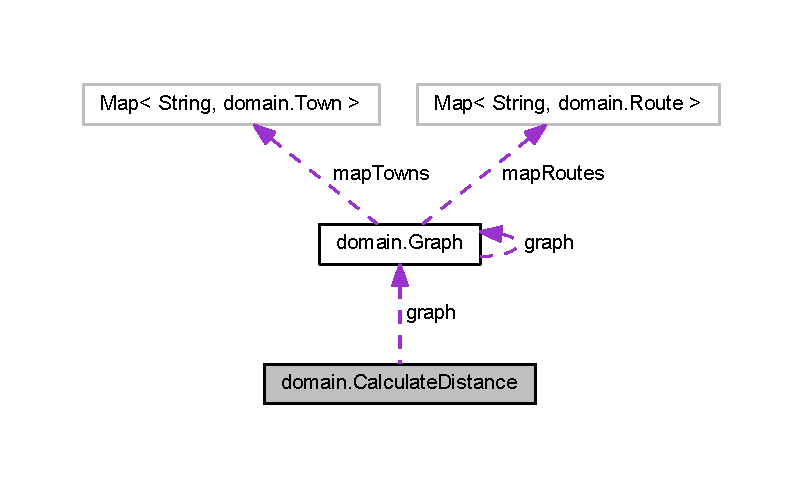
\includegraphics[width=350pt]{classdomain_1_1_calculate_distance__coll__graph}
\end{center}
\end{figure}
\subsection*{Public Member Functions}
\begin{DoxyCompactItemize}
\item 
\hyperlink{classdomain_1_1_route}{Route} \mbox{[}$\,$\mbox{]} \hyperlink{classdomain_1_1_calculate_distance_a188113ff0f6a119f4addd523b5e06a9c}{calculate\+All} ()
\end{DoxyCompactItemize}
\subsection*{Static Public Member Functions}
\begin{DoxyCompactItemize}
\item 
static \hyperlink{classdomain_1_1_route}{Route} \mbox{[}$\,$\mbox{]} \hyperlink{classdomain_1_1_calculate_distance_ad08ace3a0aa30e9ec6c99e8826630ad3}{calculate} (String\mbox{[}$\,$\mbox{]} trips)
\end{DoxyCompactItemize}
\subsection*{Static Package Attributes}
\begin{DoxyCompactItemize}
\item 
static \hyperlink{classdomain_1_1_graph}{Graph} \hyperlink{classdomain_1_1_calculate_distance_aa7288f0798e8e530b5fd8c228a7b028c}{graph} = \hyperlink{classdomain_1_1_graph_a57ce4efd344c059a565f4bb104fdee64}{Graph.\+create}()
\end{DoxyCompactItemize}


\subsection{Member Function Documentation}
\mbox{\Hypertarget{classdomain_1_1_calculate_distance_ad08ace3a0aa30e9ec6c99e8826630ad3}\label{classdomain_1_1_calculate_distance_ad08ace3a0aa30e9ec6c99e8826630ad3}} 
\index{domain\+::\+Calculate\+Distance@{domain\+::\+Calculate\+Distance}!calculate@{calculate}}
\index{calculate@{calculate}!domain\+::\+Calculate\+Distance@{domain\+::\+Calculate\+Distance}}
\subsubsection{\texorpdfstring{calculate()}{calculate()}}
{\footnotesize\ttfamily static \hyperlink{classdomain_1_1_route}{Route} \mbox{[}$\,$\mbox{]} domain.\+Calculate\+Distance.\+calculate (\begin{DoxyParamCaption}\item[{String \mbox{[}$\,$\mbox{]}}]{trips }\end{DoxyParamCaption})\hspace{0.3cm}{\ttfamily [static]}}

Calcula a distancia de uma lista de rotas(viagens)


\begin{DoxyParams}{Parameters}
{\em trips} & lista de key das rotas(viagens) para o calculo da distancia \\
\hline
\end{DoxyParams}
\begin{DoxyReturn}{Returns}
Rotas com suas respectivas distancias calculadas 
\end{DoxyReturn}
Here is the call graph for this function\+:\nopagebreak
\begin{figure}[H]
\begin{center}
\leavevmode
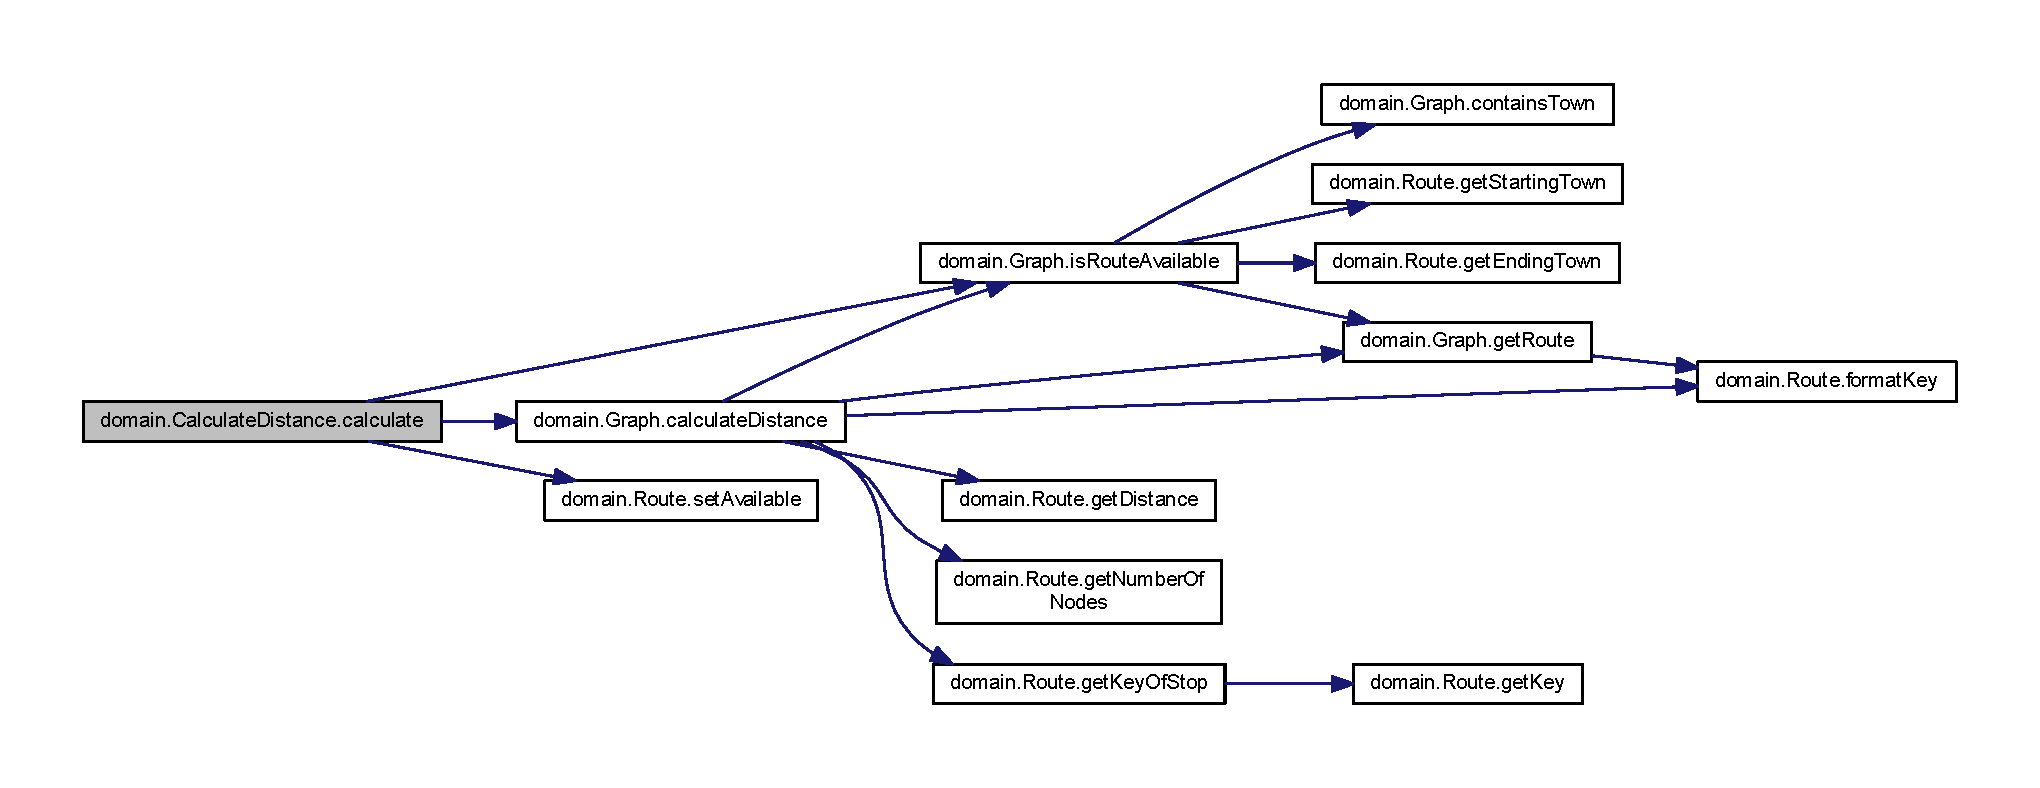
\includegraphics[width=350pt]{classdomain_1_1_calculate_distance_ad08ace3a0aa30e9ec6c99e8826630ad3_cgraph}
\end{center}
\end{figure}
Here is the caller graph for this function\+:\nopagebreak
\begin{figure}[H]
\begin{center}
\leavevmode
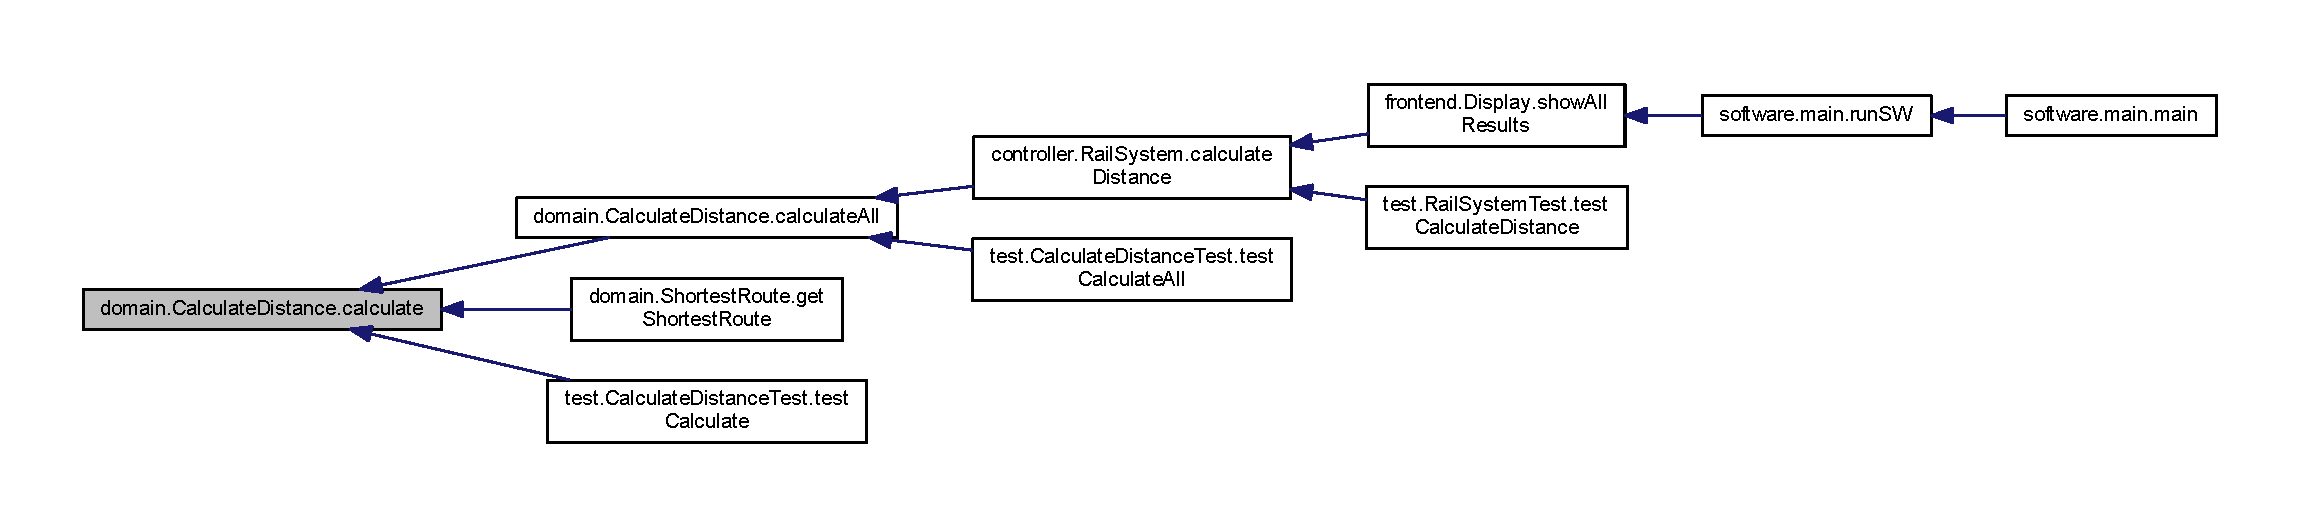
\includegraphics[width=350pt]{classdomain_1_1_calculate_distance_ad08ace3a0aa30e9ec6c99e8826630ad3_icgraph}
\end{center}
\end{figure}
\mbox{\Hypertarget{classdomain_1_1_calculate_distance_a188113ff0f6a119f4addd523b5e06a9c}\label{classdomain_1_1_calculate_distance_a188113ff0f6a119f4addd523b5e06a9c}} 
\index{domain\+::\+Calculate\+Distance@{domain\+::\+Calculate\+Distance}!calculate\+All@{calculate\+All}}
\index{calculate\+All@{calculate\+All}!domain\+::\+Calculate\+Distance@{domain\+::\+Calculate\+Distance}}
\subsubsection{\texorpdfstring{calculate\+All()}{calculateAll()}}
{\footnotesize\ttfamily \hyperlink{classdomain_1_1_route}{Route} \mbox{[}$\,$\mbox{]} domain.\+Calculate\+Distance.\+calculate\+All (\begin{DoxyParamCaption}{ }\end{DoxyParamCaption})}

Baseada na lista de rotas contida no arquivo \textquotesingle{}input.\+txt\textquotesingle{}, na proprieda \textquotesingle{}distance.\+routes\textquotesingle{}, calcula a distancia de cada uma. Rotas nao possiveis serao setada como nao existente atraves da chamada do metodo set\+Availabe(false) e o valor da distancia sera 0.\+0

\begin{DoxyReturn}{Returns}
Retorna uma lista de rotas com sua respectiva distancia calculada e com a indicacao se e uma rota possivel 
\end{DoxyReturn}
Here is the call graph for this function\+:\nopagebreak
\begin{figure}[H]
\begin{center}
\leavevmode
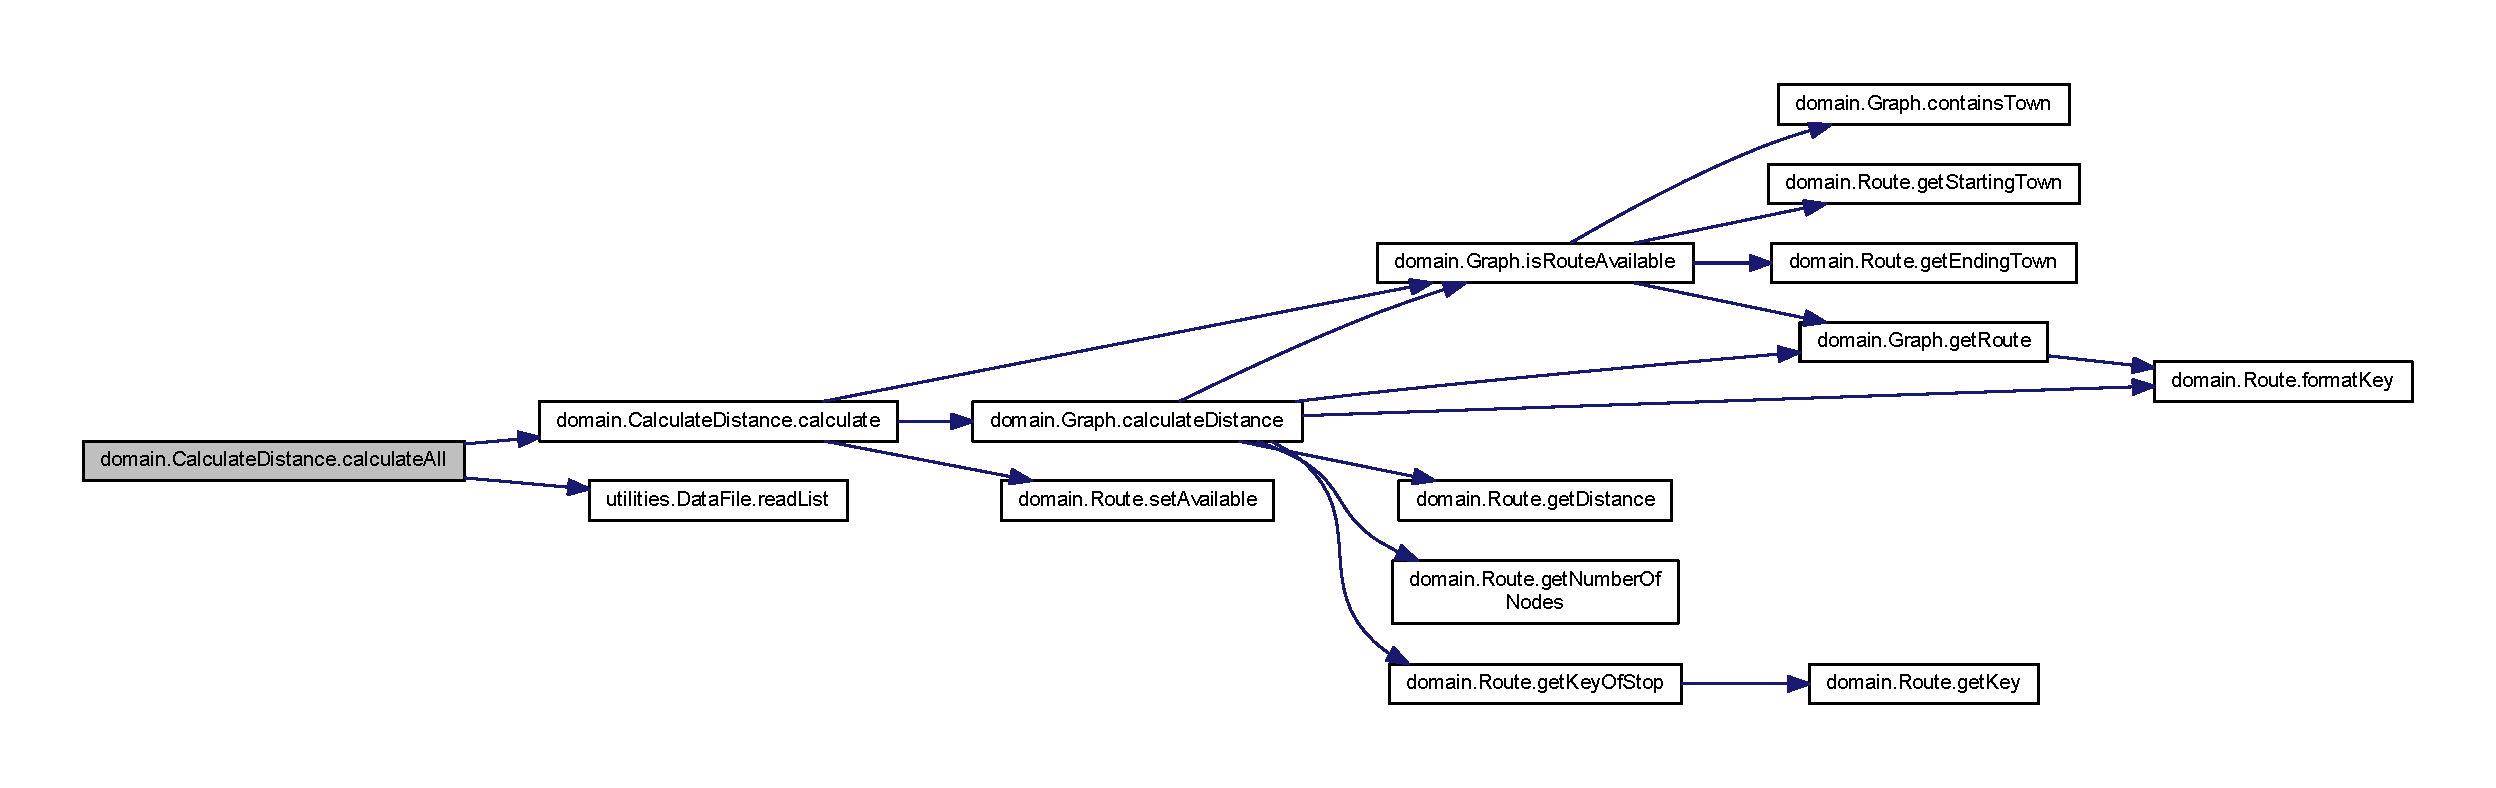
\includegraphics[width=350pt]{classdomain_1_1_calculate_distance_a188113ff0f6a119f4addd523b5e06a9c_cgraph}
\end{center}
\end{figure}
Here is the caller graph for this function\+:\nopagebreak
\begin{figure}[H]
\begin{center}
\leavevmode
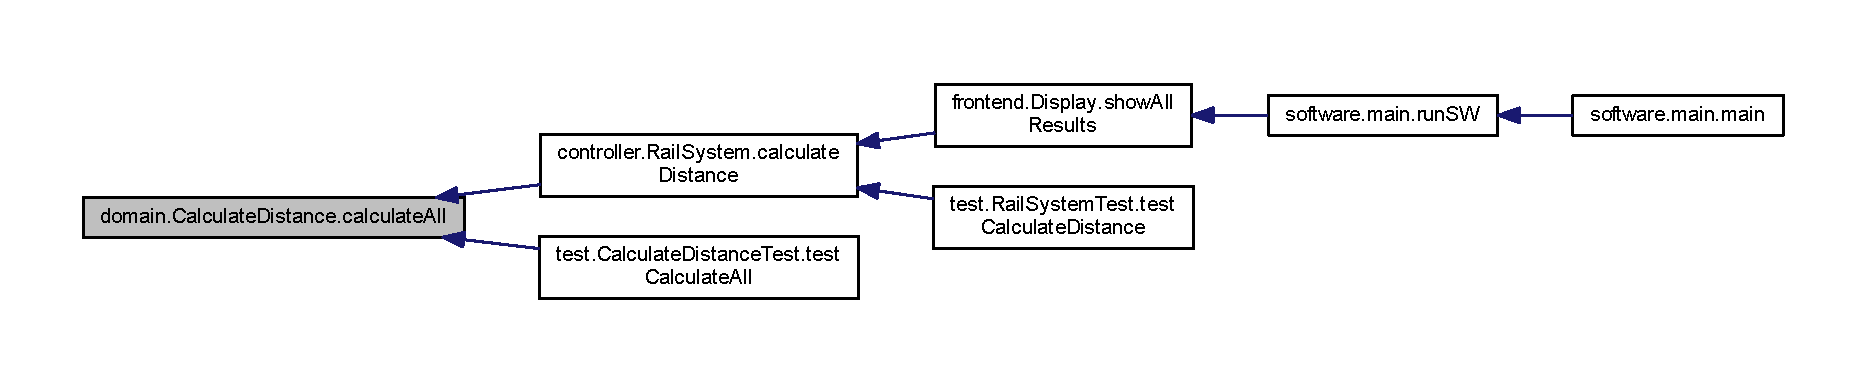
\includegraphics[width=350pt]{classdomain_1_1_calculate_distance_a188113ff0f6a119f4addd523b5e06a9c_icgraph}
\end{center}
\end{figure}


\subsection{Member Data Documentation}
\mbox{\Hypertarget{classdomain_1_1_calculate_distance_aa7288f0798e8e530b5fd8c228a7b028c}\label{classdomain_1_1_calculate_distance_aa7288f0798e8e530b5fd8c228a7b028c}} 
\index{domain\+::\+Calculate\+Distance@{domain\+::\+Calculate\+Distance}!graph@{graph}}
\index{graph@{graph}!domain\+::\+Calculate\+Distance@{domain\+::\+Calculate\+Distance}}
\subsubsection{\texorpdfstring{graph}{graph}}
{\footnotesize\ttfamily \hyperlink{classdomain_1_1_graph}{Graph} domain.\+Calculate\+Distance.\+graph = \hyperlink{classdomain_1_1_graph_a57ce4efd344c059a565f4bb104fdee64}{Graph.\+create}()\hspace{0.3cm}{\ttfamily [static]}, {\ttfamily [package]}}

Rotas disponiveis no sistema 

The documentation for this class was generated from the following file\+:\begin{DoxyCompactItemize}
\item 
D\+:/workspace/\+Train\+Vagas/src/domain/\hyperlink{_calculate_distance_8java}{Calculate\+Distance.\+java}\end{DoxyCompactItemize}

\hypertarget{classtest_1_1_calculate_distance_test}{}\section{test.\+Calculate\+Distance\+Test Class Reference}
\label{classtest_1_1_calculate_distance_test}\index{test.\+Calculate\+Distance\+Test@{test.\+Calculate\+Distance\+Test}}


Collaboration diagram for test.\+Calculate\+Distance\+Test\+:\nopagebreak
\begin{figure}[H]
\begin{center}
\leavevmode
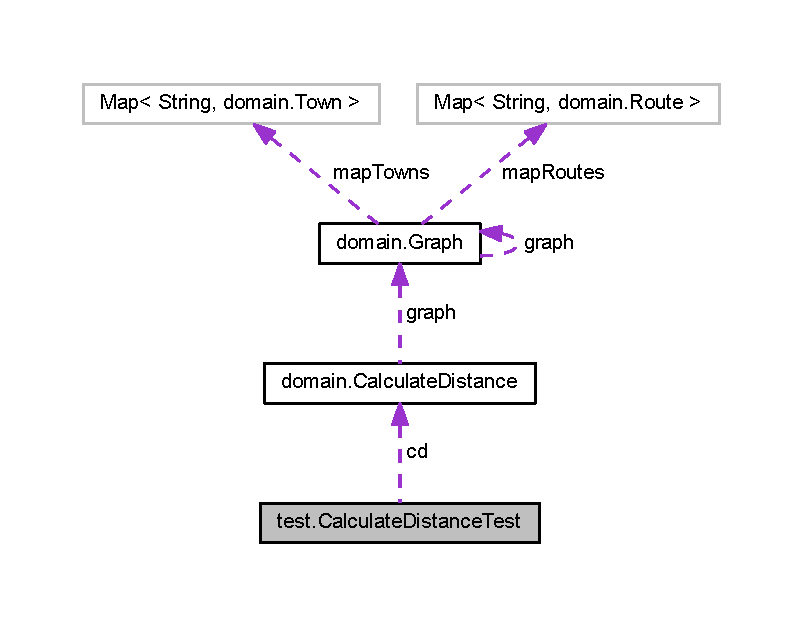
\includegraphics[width=350pt]{classtest_1_1_calculate_distance_test__coll__graph}
\end{center}
\end{figure}
\subsection*{Public Member Functions}
\begin{DoxyCompactItemize}
\item 
void \hyperlink{classtest_1_1_calculate_distance_test_a6af11430659ffdfbf1f30b96b68bf642}{set\+Up} ()  throws Exception 
\item 
void \hyperlink{classtest_1_1_calculate_distance_test_ad6642d43b502c0bf9bd3876fc3303d14}{test\+Calculate\+All} ()
\item 
void \hyperlink{classtest_1_1_calculate_distance_test_ae21407ac9f926798d08a69dfdbb6fcbe}{test\+Calculate} ()
\end{DoxyCompactItemize}
\subsection*{Package Attributes}
\begin{DoxyCompactItemize}
\item 
\hyperlink{classdomain_1_1_calculate_distance}{Calculate\+Distance} \hyperlink{classtest_1_1_calculate_distance_test_aed188a5511ba8e51661627c7ec48bd00}{cd}
\end{DoxyCompactItemize}


\subsection{Member Function Documentation}
\mbox{\Hypertarget{classtest_1_1_calculate_distance_test_a6af11430659ffdfbf1f30b96b68bf642}\label{classtest_1_1_calculate_distance_test_a6af11430659ffdfbf1f30b96b68bf642}} 
\index{test\+::\+Calculate\+Distance\+Test@{test\+::\+Calculate\+Distance\+Test}!set\+Up@{set\+Up}}
\index{set\+Up@{set\+Up}!test\+::\+Calculate\+Distance\+Test@{test\+::\+Calculate\+Distance\+Test}}
\subsubsection{\texorpdfstring{set\+Up()}{setUp()}}
{\footnotesize\ttfamily void test.\+Calculate\+Distance\+Test.\+set\+Up (\begin{DoxyParamCaption}{ }\end{DoxyParamCaption}) throws Exception}

Here is the call graph for this function\+:\nopagebreak
\begin{figure}[H]
\begin{center}
\leavevmode
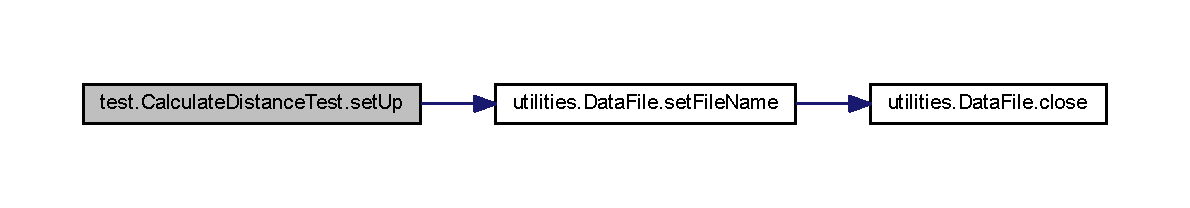
\includegraphics[width=350pt]{classtest_1_1_calculate_distance_test_a6af11430659ffdfbf1f30b96b68bf642_cgraph}
\end{center}
\end{figure}
\mbox{\Hypertarget{classtest_1_1_calculate_distance_test_ae21407ac9f926798d08a69dfdbb6fcbe}\label{classtest_1_1_calculate_distance_test_ae21407ac9f926798d08a69dfdbb6fcbe}} 
\index{test\+::\+Calculate\+Distance\+Test@{test\+::\+Calculate\+Distance\+Test}!test\+Calculate@{test\+Calculate}}
\index{test\+Calculate@{test\+Calculate}!test\+::\+Calculate\+Distance\+Test@{test\+::\+Calculate\+Distance\+Test}}
\subsubsection{\texorpdfstring{test\+Calculate()}{testCalculate()}}
{\footnotesize\ttfamily void test.\+Calculate\+Distance\+Test.\+test\+Calculate (\begin{DoxyParamCaption}{ }\end{DoxyParamCaption})}

Here is the call graph for this function\+:\nopagebreak
\begin{figure}[H]
\begin{center}
\leavevmode
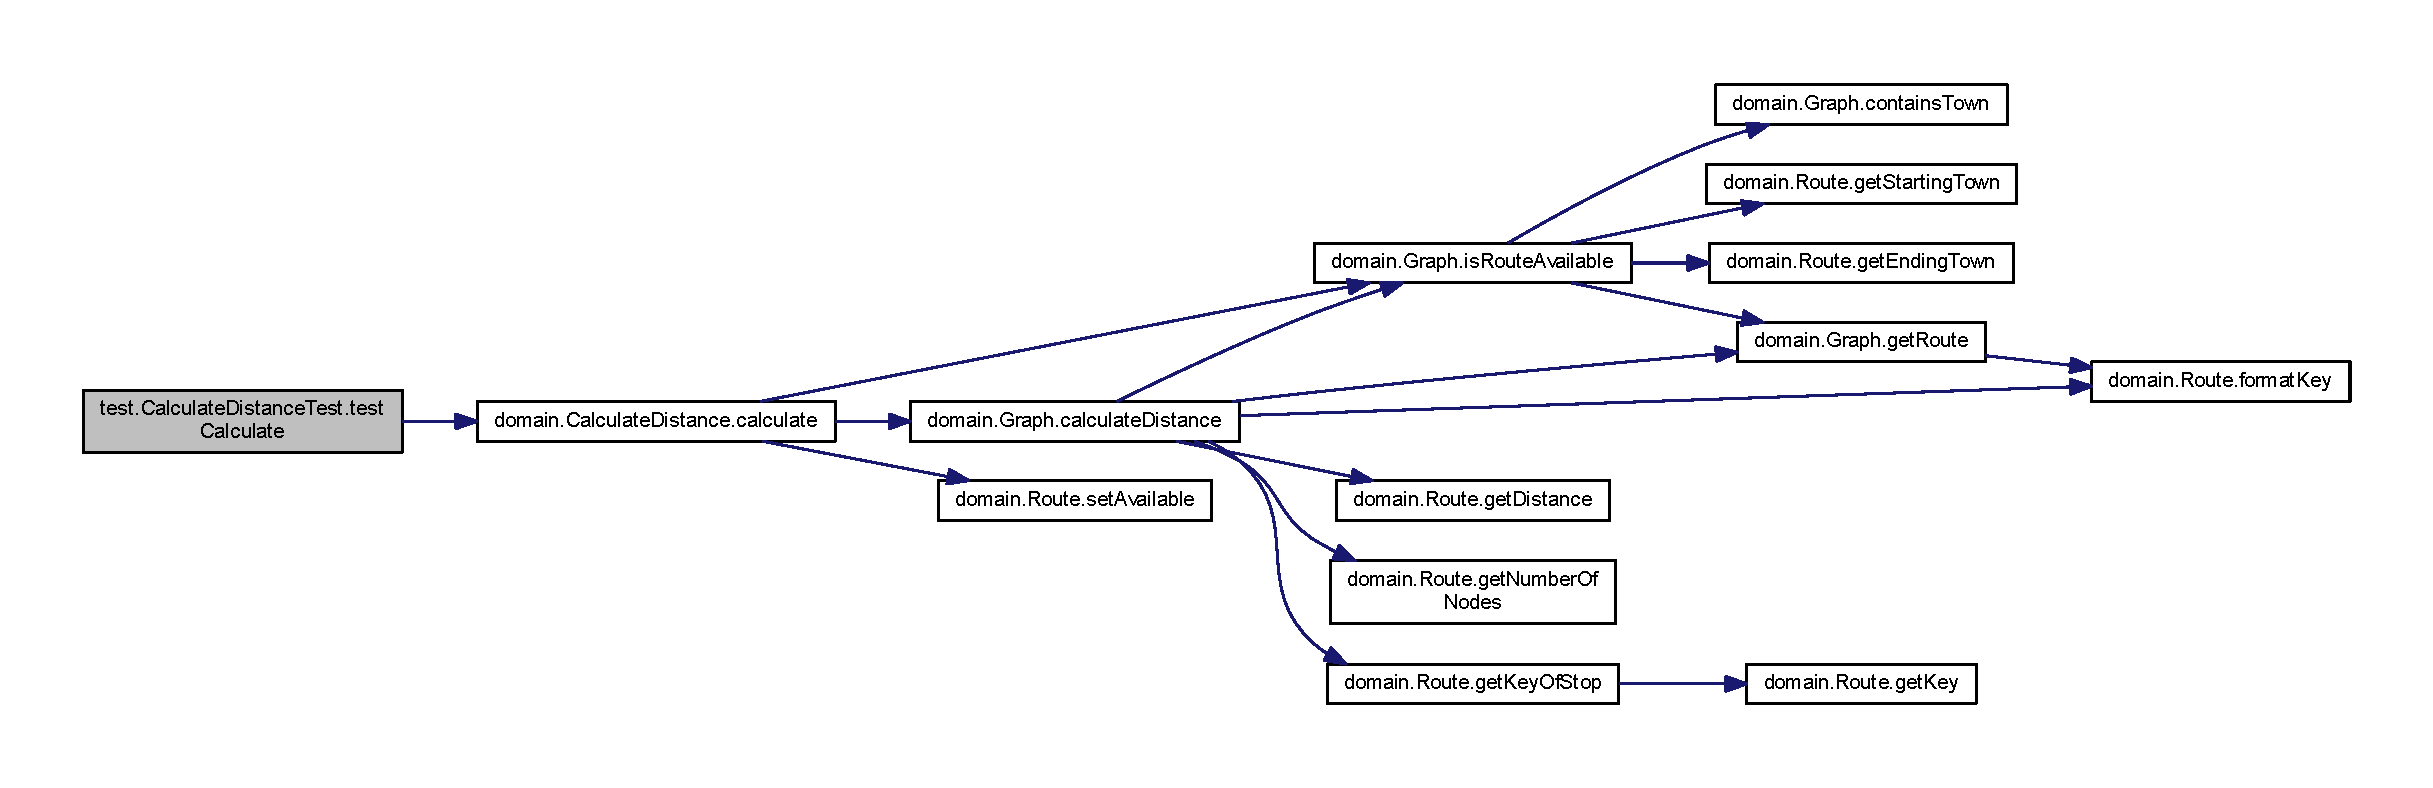
\includegraphics[width=350pt]{classtest_1_1_calculate_distance_test_ae21407ac9f926798d08a69dfdbb6fcbe_cgraph}
\end{center}
\end{figure}
\mbox{\Hypertarget{classtest_1_1_calculate_distance_test_ad6642d43b502c0bf9bd3876fc3303d14}\label{classtest_1_1_calculate_distance_test_ad6642d43b502c0bf9bd3876fc3303d14}} 
\index{test\+::\+Calculate\+Distance\+Test@{test\+::\+Calculate\+Distance\+Test}!test\+Calculate\+All@{test\+Calculate\+All}}
\index{test\+Calculate\+All@{test\+Calculate\+All}!test\+::\+Calculate\+Distance\+Test@{test\+::\+Calculate\+Distance\+Test}}
\subsubsection{\texorpdfstring{test\+Calculate\+All()}{testCalculateAll()}}
{\footnotesize\ttfamily void test.\+Calculate\+Distance\+Test.\+test\+Calculate\+All (\begin{DoxyParamCaption}{ }\end{DoxyParamCaption})}

Here is the call graph for this function\+:\nopagebreak
\begin{figure}[H]
\begin{center}
\leavevmode
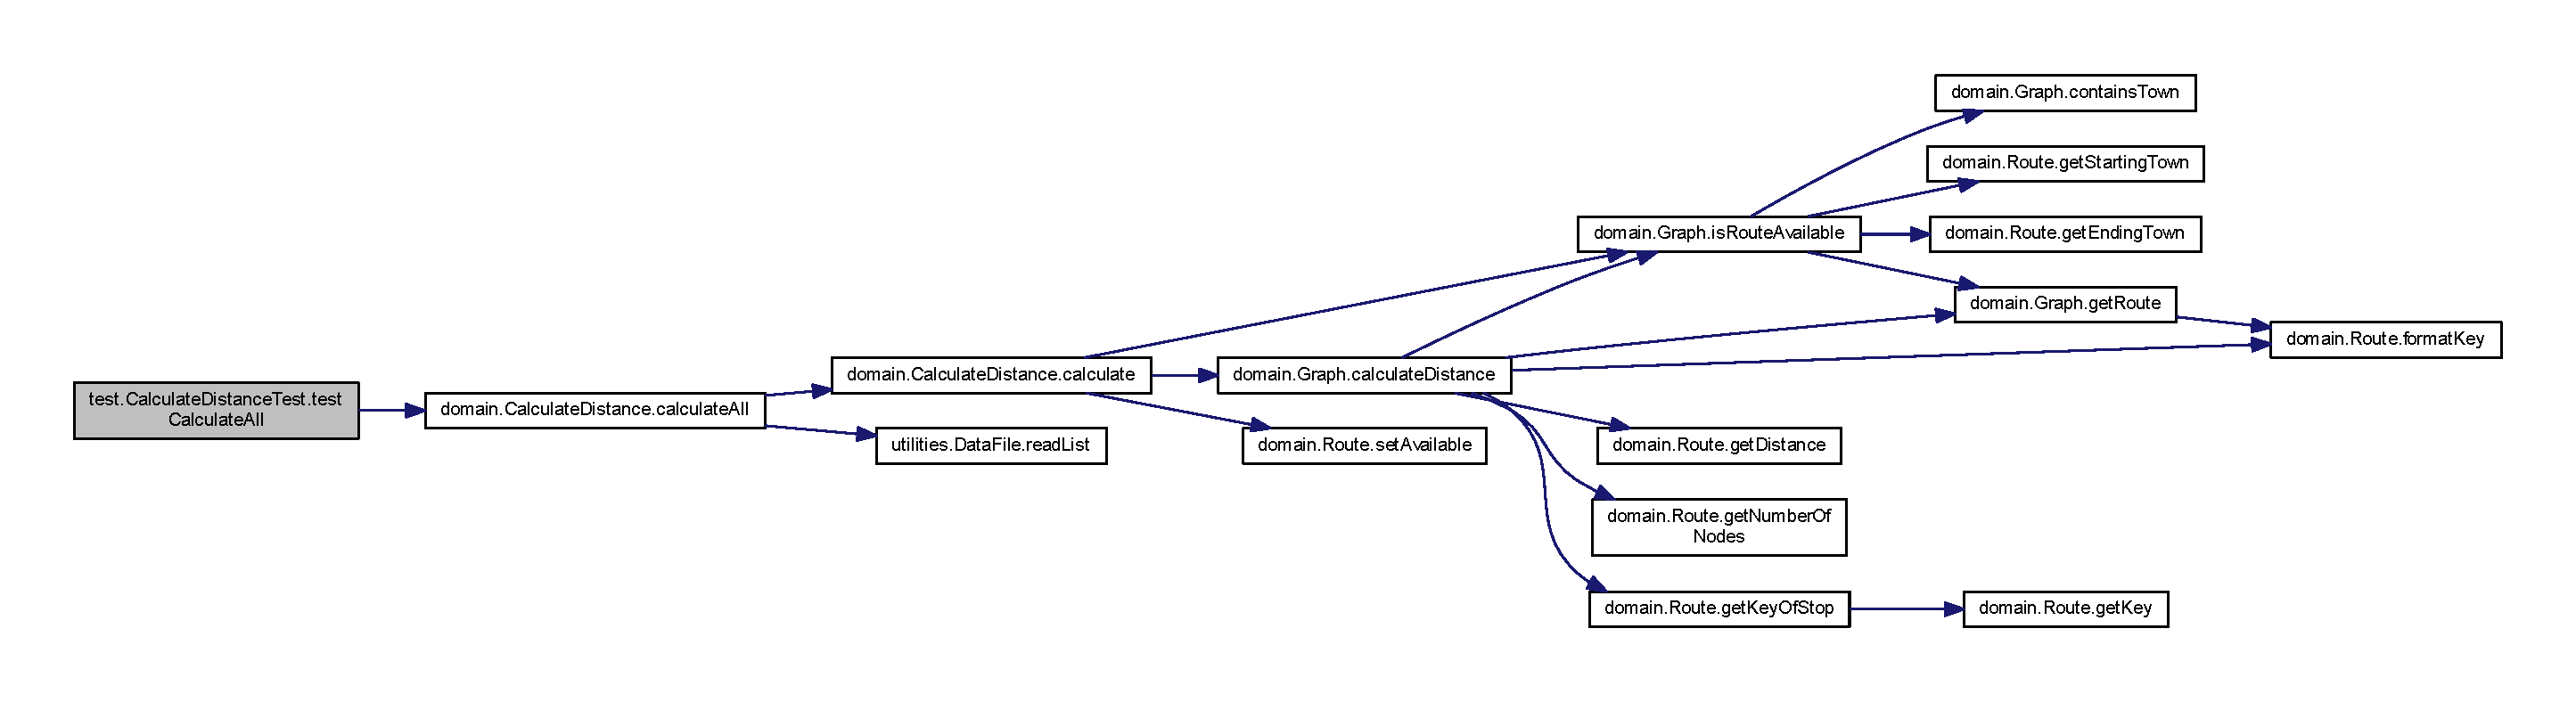
\includegraphics[width=350pt]{classtest_1_1_calculate_distance_test_ad6642d43b502c0bf9bd3876fc3303d14_cgraph}
\end{center}
\end{figure}


\subsection{Member Data Documentation}
\mbox{\Hypertarget{classtest_1_1_calculate_distance_test_aed188a5511ba8e51661627c7ec48bd00}\label{classtest_1_1_calculate_distance_test_aed188a5511ba8e51661627c7ec48bd00}} 
\index{test\+::\+Calculate\+Distance\+Test@{test\+::\+Calculate\+Distance\+Test}!cd@{cd}}
\index{cd@{cd}!test\+::\+Calculate\+Distance\+Test@{test\+::\+Calculate\+Distance\+Test}}
\subsubsection{\texorpdfstring{cd}{cd}}
{\footnotesize\ttfamily \hyperlink{classdomain_1_1_calculate_distance}{Calculate\+Distance} test.\+Calculate\+Distance\+Test.\+cd\hspace{0.3cm}{\ttfamily [package]}}



The documentation for this class was generated from the following file\+:\begin{DoxyCompactItemize}
\item 
D\+:/workspace/\+Train\+Vagas/src/test/\hyperlink{_calculate_distance_test_8java}{Calculate\+Distance\+Test.\+java}\end{DoxyCompactItemize}

\hypertarget{classutilities_1_1_data_file}{}\section{utilities.\+Data\+File Class Reference}
\label{classutilities_1_1_data_file}\index{utilities.\+Data\+File@{utilities.\+Data\+File}}


Collaboration diagram for utilities.\+Data\+File\+:\nopagebreak
\begin{figure}[H]
\begin{center}
\leavevmode
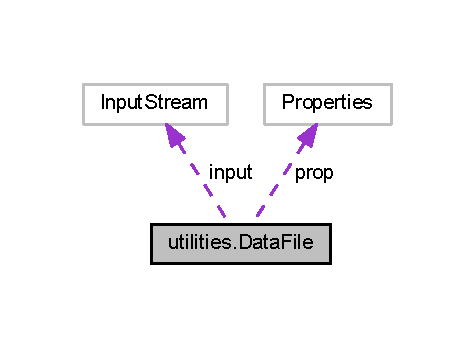
\includegraphics[width=228pt]{classutilities_1_1_data_file__coll__graph}
\end{center}
\end{figure}
\subsection*{Static Public Member Functions}
\begin{DoxyCompactItemize}
\item 
static void \hyperlink{classutilities_1_1_data_file_a03d4af9888db5dfd5031fd3ead4964bf}{set\+File\+Name} (String file)
\item 
static String \hyperlink{classutilities_1_1_data_file_ae5e95d9019f786414f891e2afc966381}{get\+File\+Name} ()
\item 
static boolean \hyperlink{classutilities_1_1_data_file_aa53fb6327a320f458fd8314751e241c9}{open} ()
\item 
static void \hyperlink{classutilities_1_1_data_file_a4f113f0a5f50902308585d1f11988ec7}{close} ()
\item 
static String \mbox{[}$\,$\mbox{]} \hyperlink{classutilities_1_1_data_file_a68332bb2b70bafbaae007d952ba4264b}{read\+List} (\hyperlink{enumutilities_1_1_file_property}{File\+Property} property)
\item 
static String \mbox{[}$\,$\mbox{]} \hyperlink{classutilities_1_1_data_file_a86acc1699af206a96ab51c94d6663afe}{read\+List} (\hyperlink{enumutilities_1_1_file_property}{File\+Property} property, int index\+\_\+filter)
\item 
static String \hyperlink{classutilities_1_1_data_file_ae44a128705ef07c67393153806fb5216}{read\+Condition} (\hyperlink{enumutilities_1_1_file_property}{File\+Property} property, int index\+\_\+filter)
\item 
static double \hyperlink{classutilities_1_1_data_file_aafa9fbee5003c8d9abcd0b02ba4b31dc}{read\+Double} (\hyperlink{enumutilities_1_1_file_property}{File\+Property} property, int index\+\_\+filter)
\item 
static int \hyperlink{classutilities_1_1_data_file_a7576f90d40db372f262216f8f6a64c28}{read\+Integer} (\hyperlink{enumutilities_1_1_file_property}{File\+Property} property, int index\+\_\+filter)
\item 
static String \hyperlink{classutilities_1_1_data_file_adb4c1c9272d3497615385f4f8278ab60}{read\+Literal\+Operand} (\hyperlink{enumutilities_1_1_file_property}{File\+Property} property, int index\+\_\+filter)
\item 
static boolean \hyperlink{classutilities_1_1_data_file_a28beb850c6cc447aa7757e9f3967224c}{check\+File\+Exist} ()
\end{DoxyCompactItemize}
\subsection*{Static Public Attributes}
\begin{DoxyCompactItemize}
\item 
static final int \hyperlink{classutilities_1_1_data_file_a7db48e719d69b2fb08dec6730949acf9}{D\+I\+S\+T\+A\+N\+C\+E\+\_\+\+C\+O\+N\+D\+I\+T\+I\+ON} =3
\item 
static final int \hyperlink{classutilities_1_1_data_file_a73169a0777ef2c7e224420ab3f4be9dc}{S\+T\+O\+P1\+\_\+\+C\+O\+N\+D\+I\+T\+I\+ON} =1
\item 
static final int \hyperlink{classutilities_1_1_data_file_afdb877fcbb93d5bf2e6757f844c0a0e0}{S\+T\+O\+P2\+\_\+\+C\+O\+N\+D\+I\+T\+I\+ON} =2
\item 
static final String \hyperlink{classutilities_1_1_data_file_ab2cdae484f28934cf77316bbf9af0b72}{P\+A\+T\+H\+\_\+\+F\+I\+LE} = \char`\"{}input.\+txt\char`\"{}
\item 
static final String \hyperlink{classutilities_1_1_data_file_a6d7f06ae7db77b3b202c31190c2281e3}{F\+I\+L\+E\+\_\+\+T\+E\+S\+T\+S\+\_\+\+C\+A\+S\+ES} = \char`\"{}F\+I\+L\+E\+\_\+\+T\+E\+S\+T\+\_\+\+C\+A\+S\+E.\+txt\char`\"{}
\end{DoxyCompactItemize}
\subsection*{Static Package Attributes}
\begin{DoxyCompactItemize}
\item 
static Properties \hyperlink{classutilities_1_1_data_file_a56e3023d87523528a6126799b02b089d}{prop} = new Properties()
\item 
static Input\+Stream \hyperlink{classutilities_1_1_data_file_a80202aa4edd480f4404d9fd4adcedbfc}{input} = null
\end{DoxyCompactItemize}
\subsection*{Static Private Attributes}
\begin{DoxyCompactItemize}
\item 
static final String \hyperlink{classutilities_1_1_data_file_a25b4360923bcdd2e38e81df53297ee94}{P\+A\+T\+T\+E\+R\+N\+\_\+\+L\+I\+ST} =\char`\"{}\mbox{[}$^\wedge$a-\/zA-\/Z0-\/9.,\mbox{]}\char`\"{}
\item 
static final String \hyperlink{classutilities_1_1_data_file_aeb2abc62f5fe561e1425331c49c1a58d}{P\+A\+T\+T\+E\+R\+N\+\_\+\+O\+P\+E\+R\+A\+ND} =\char`\"{}\mbox{[}$^\wedge$a-\/zA-\/Z,\mbox{]}\char`\"{}
\item 
static final String \hyperlink{classutilities_1_1_data_file_ac00c547e129cb9c057f7a0d499015797}{P\+A\+T\+T\+E\+R\+N\+\_\+\+D\+O\+U\+B\+LE} =\char`\"{}\mbox{[}$^\wedge$0-\/9.,\mbox{]}\char`\"{}
\item 
static final String \hyperlink{classutilities_1_1_data_file_a51e037b86bf7cd4b6ce02a384d9ad6f2}{P\+A\+T\+T\+E\+R\+N\+\_\+\+I\+N\+T\+E\+G\+ER} =\char`\"{}\mbox{[}$^\wedge$0-\/9\mbox{]}\char`\"{}
\item 
static final String \hyperlink{classutilities_1_1_data_file_aee831317a6c670d621683dbfadf1d19f}{P\+A\+T\+T\+E\+R\+N\+\_\+\+C\+O\+N\+D\+I\+T\+I\+ON} =\char`\"{}\mbox{[}$^\wedge$$<$$>$=!\mbox{]}\char`\"{}
\item 
static final String \hyperlink{classutilities_1_1_data_file_ae7a89abc44a0f02d5b6205b6e2f53a06}{S\+E\+P\+A\+R\+A\+T\+OR} =\char`\"{},\char`\"{}
\item 
static String \hyperlink{classutilities_1_1_data_file_acc01b0a1464087e54962b7c6202dbb5f}{file\+\_\+name} = \hyperlink{classutilities_1_1_data_file_ab2cdae484f28934cf77316bbf9af0b72}{P\+A\+T\+H\+\_\+\+F\+I\+LE}
\end{DoxyCompactItemize}


\subsection{Member Function Documentation}
\mbox{\Hypertarget{classutilities_1_1_data_file_a28beb850c6cc447aa7757e9f3967224c}\label{classutilities_1_1_data_file_a28beb850c6cc447aa7757e9f3967224c}} 
\index{utilities\+::\+Data\+File@{utilities\+::\+Data\+File}!check\+File\+Exist@{check\+File\+Exist}}
\index{check\+File\+Exist@{check\+File\+Exist}!utilities\+::\+Data\+File@{utilities\+::\+Data\+File}}
\subsubsection{\texorpdfstring{check\+File\+Exist()}{checkFileExist()}}
{\footnotesize\ttfamily static boolean utilities.\+Data\+File.\+check\+File\+Exist (\begin{DoxyParamCaption}{ }\end{DoxyParamCaption})\hspace{0.3cm}{\ttfamily [static]}}

Here is the caller graph for this function\+:\nopagebreak
\begin{figure}[H]
\begin{center}
\leavevmode
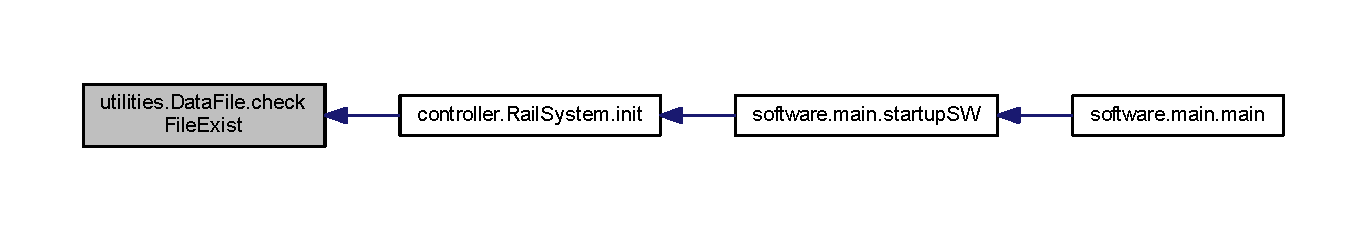
\includegraphics[width=350pt]{classutilities_1_1_data_file_a28beb850c6cc447aa7757e9f3967224c_icgraph}
\end{center}
\end{figure}
\mbox{\Hypertarget{classutilities_1_1_data_file_a4f113f0a5f50902308585d1f11988ec7}\label{classutilities_1_1_data_file_a4f113f0a5f50902308585d1f11988ec7}} 
\index{utilities\+::\+Data\+File@{utilities\+::\+Data\+File}!close@{close}}
\index{close@{close}!utilities\+::\+Data\+File@{utilities\+::\+Data\+File}}
\subsubsection{\texorpdfstring{close()}{close()}}
{\footnotesize\ttfamily static void utilities.\+Data\+File.\+close (\begin{DoxyParamCaption}{ }\end{DoxyParamCaption})\hspace{0.3cm}{\ttfamily [static]}}

Fecha o arquivo de entrada Here is the caller graph for this function\+:\nopagebreak
\begin{figure}[H]
\begin{center}
\leavevmode
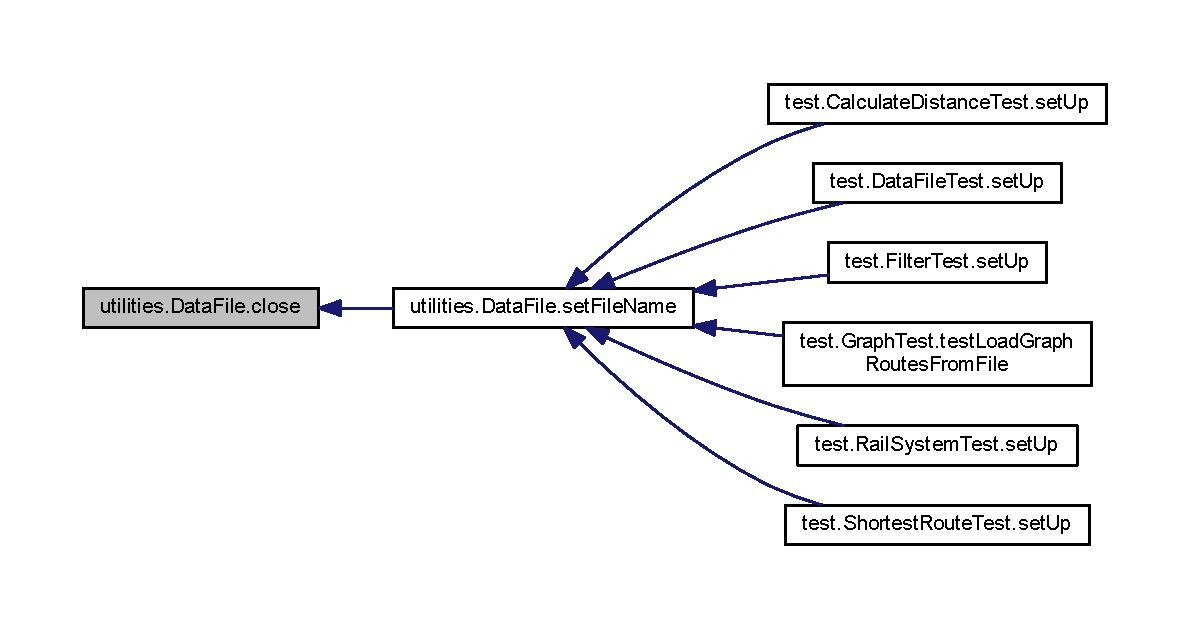
\includegraphics[width=350pt]{classutilities_1_1_data_file_a4f113f0a5f50902308585d1f11988ec7_icgraph}
\end{center}
\end{figure}
\mbox{\Hypertarget{classutilities_1_1_data_file_ae5e95d9019f786414f891e2afc966381}\label{classutilities_1_1_data_file_ae5e95d9019f786414f891e2afc966381}} 
\index{utilities\+::\+Data\+File@{utilities\+::\+Data\+File}!get\+File\+Name@{get\+File\+Name}}
\index{get\+File\+Name@{get\+File\+Name}!utilities\+::\+Data\+File@{utilities\+::\+Data\+File}}
\subsubsection{\texorpdfstring{get\+File\+Name()}{getFileName()}}
{\footnotesize\ttfamily static String utilities.\+Data\+File.\+get\+File\+Name (\begin{DoxyParamCaption}{ }\end{DoxyParamCaption})\hspace{0.3cm}{\ttfamily [static]}}

\begin{DoxyReturn}{Returns}
Retorna nome do arquivo em uso 
\end{DoxyReturn}
Here is the caller graph for this function\+:\nopagebreak
\begin{figure}[H]
\begin{center}
\leavevmode
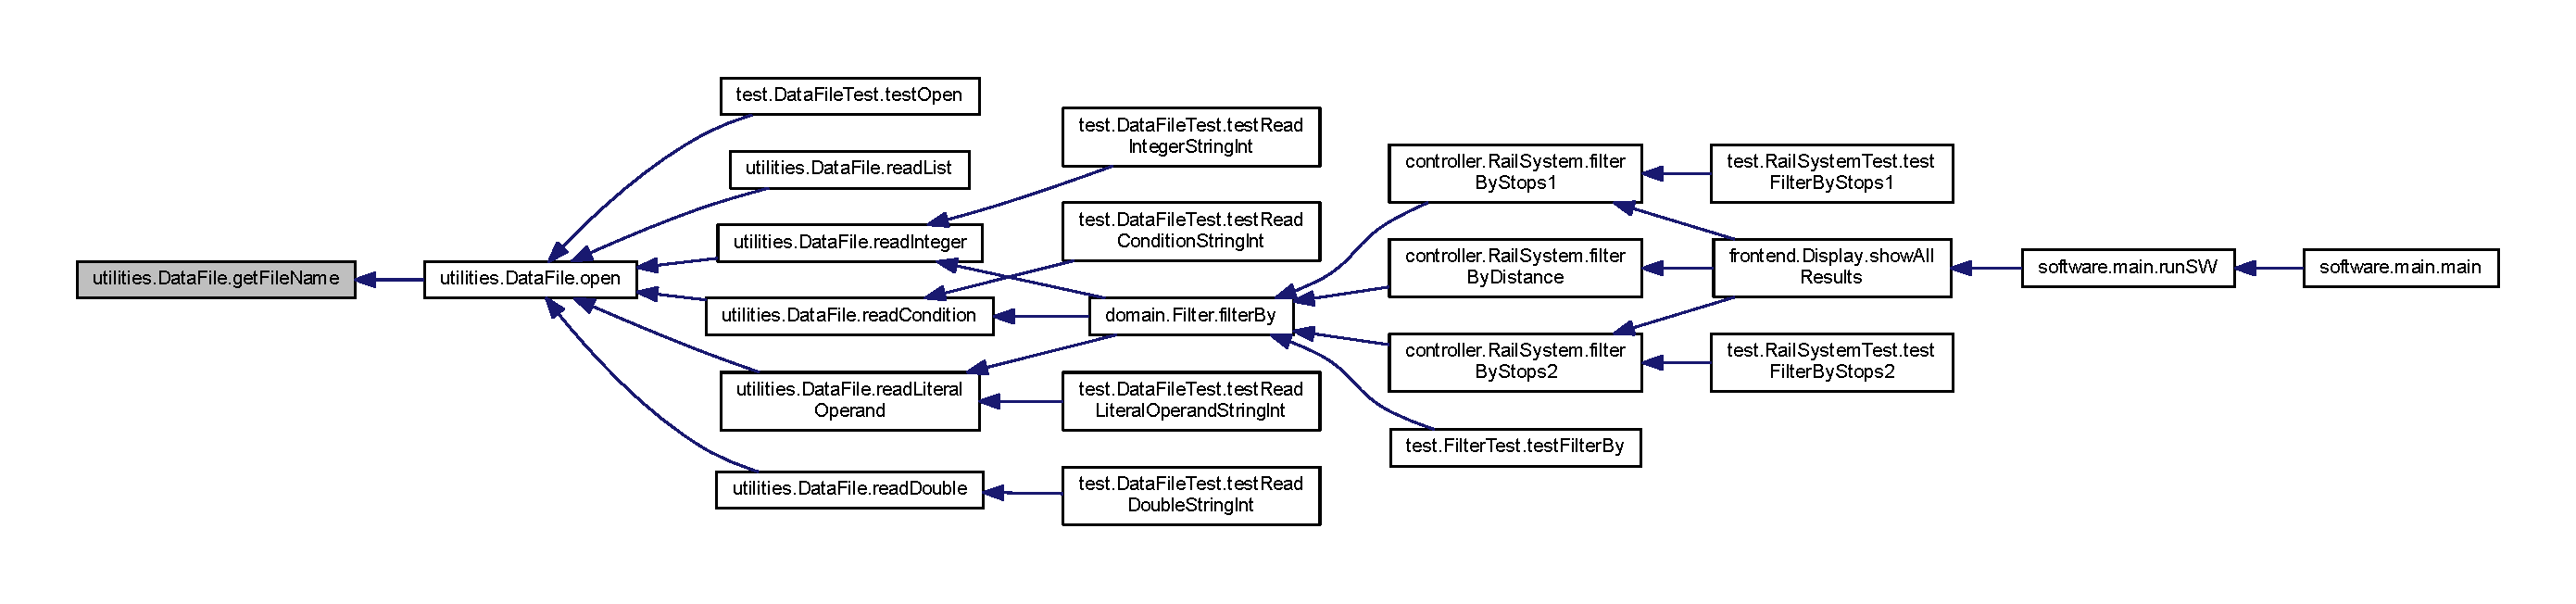
\includegraphics[width=350pt]{classutilities_1_1_data_file_ae5e95d9019f786414f891e2afc966381_icgraph}
\end{center}
\end{figure}
\mbox{\Hypertarget{classutilities_1_1_data_file_aa53fb6327a320f458fd8314751e241c9}\label{classutilities_1_1_data_file_aa53fb6327a320f458fd8314751e241c9}} 
\index{utilities\+::\+Data\+File@{utilities\+::\+Data\+File}!open@{open}}
\index{open@{open}!utilities\+::\+Data\+File@{utilities\+::\+Data\+File}}
\subsubsection{\texorpdfstring{open()}{open()}}
{\footnotesize\ttfamily static boolean utilities.\+Data\+File.\+open (\begin{DoxyParamCaption}{ }\end{DoxyParamCaption})\hspace{0.3cm}{\ttfamily [static]}}

Abre o arquivo de entrada \begin{DoxyReturn}{Returns}
Se o arquivo foi aberto com sucesso retorna true 
\end{DoxyReturn}
Here is the call graph for this function\+:\nopagebreak
\begin{figure}[H]
\begin{center}
\leavevmode
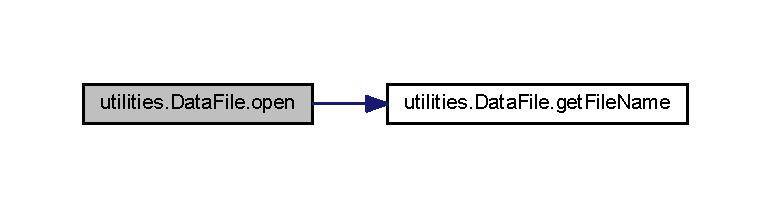
\includegraphics[width=350pt]{classutilities_1_1_data_file_aa53fb6327a320f458fd8314751e241c9_cgraph}
\end{center}
\end{figure}
Here is the caller graph for this function\+:\nopagebreak
\begin{figure}[H]
\begin{center}
\leavevmode
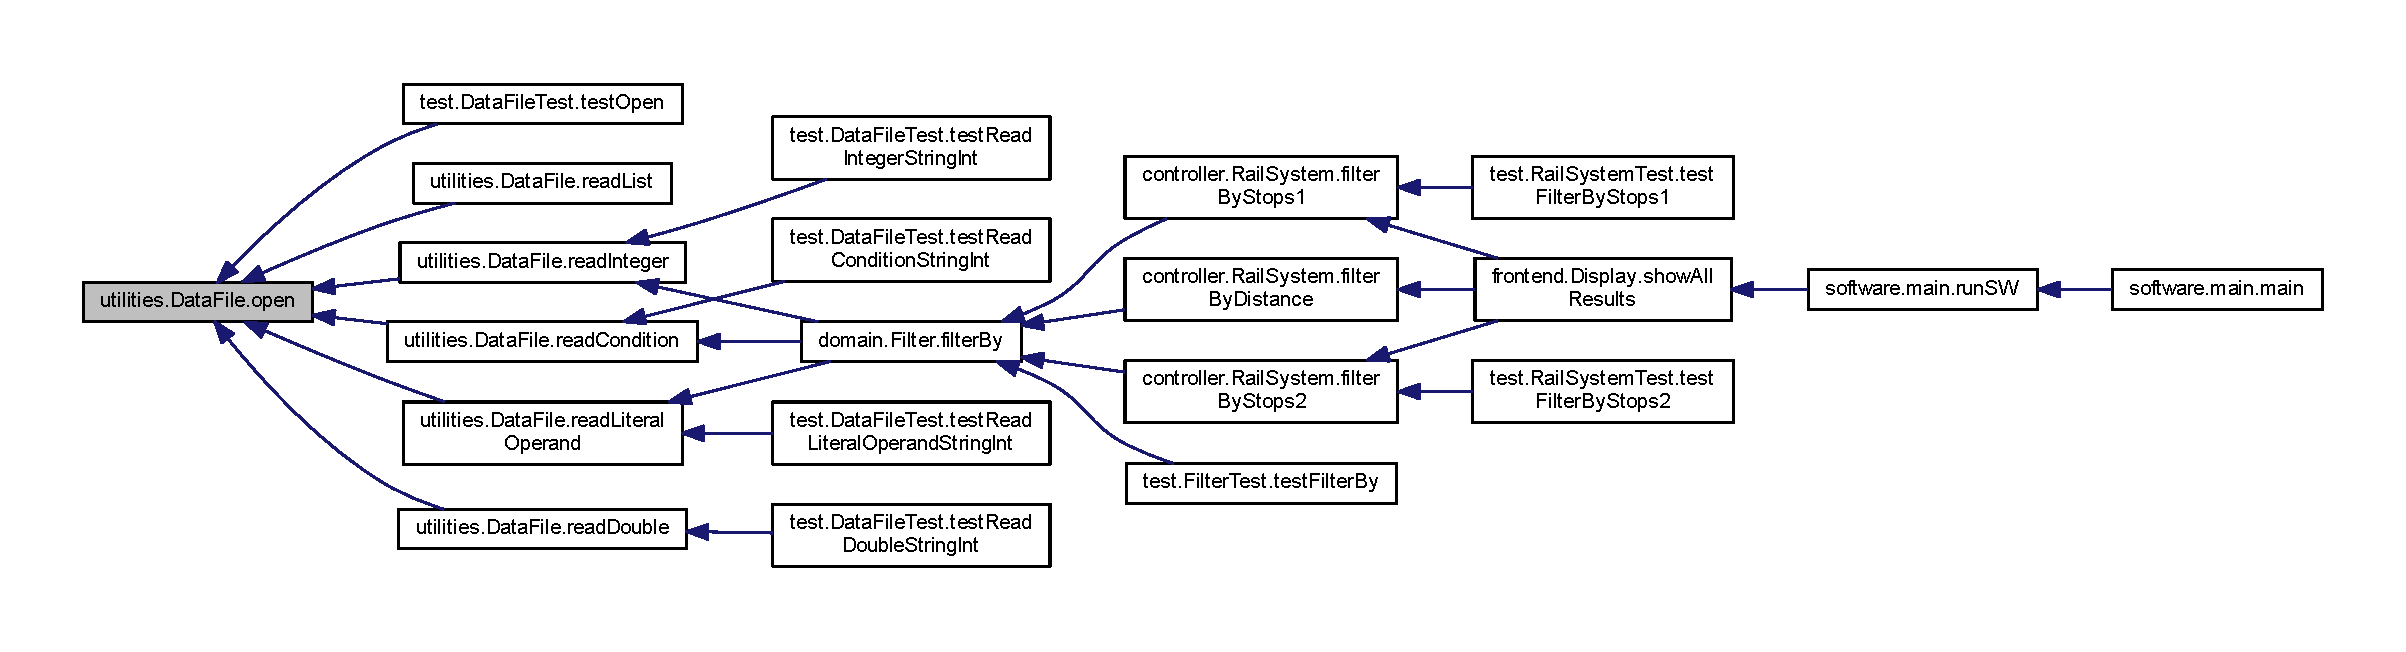
\includegraphics[width=350pt]{classutilities_1_1_data_file_aa53fb6327a320f458fd8314751e241c9_icgraph}
\end{center}
\end{figure}
\mbox{\Hypertarget{classutilities_1_1_data_file_ae44a128705ef07c67393153806fb5216}\label{classutilities_1_1_data_file_ae44a128705ef07c67393153806fb5216}} 
\index{utilities\+::\+Data\+File@{utilities\+::\+Data\+File}!read\+Condition@{read\+Condition}}
\index{read\+Condition@{read\+Condition}!utilities\+::\+Data\+File@{utilities\+::\+Data\+File}}
\subsubsection{\texorpdfstring{read\+Condition()}{readCondition()}}
{\footnotesize\ttfamily static String utilities.\+Data\+File.\+read\+Condition (\begin{DoxyParamCaption}\item[{\hyperlink{enumutilities_1_1_file_property}{File\+Property}}]{property,  }\item[{int}]{index\+\_\+filter }\end{DoxyParamCaption})\hspace{0.3cm}{\ttfamily [static]}}

Le uma condicao do arquivo de entrada 
\begin{DoxyParams}{Parameters}
{\em property} & propriedade onde a condicao sera buscado \\
\hline
{\em index\+\_\+filter} & index da propriedade a ser buscada ex\+: propriedade\mbox{[}index\mbox{]}.condition \\
\hline
\end{DoxyParams}
\begin{DoxyReturn}{Returns}
retorna a condicao literal lido do arquivo 
\end{DoxyReturn}
Here is the call graph for this function\+:\nopagebreak
\begin{figure}[H]
\begin{center}
\leavevmode
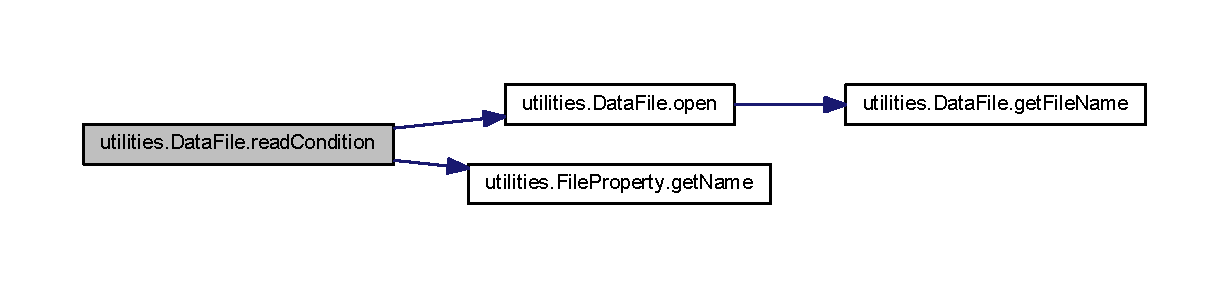
\includegraphics[width=350pt]{classutilities_1_1_data_file_ae44a128705ef07c67393153806fb5216_cgraph}
\end{center}
\end{figure}
Here is the caller graph for this function\+:\nopagebreak
\begin{figure}[H]
\begin{center}
\leavevmode
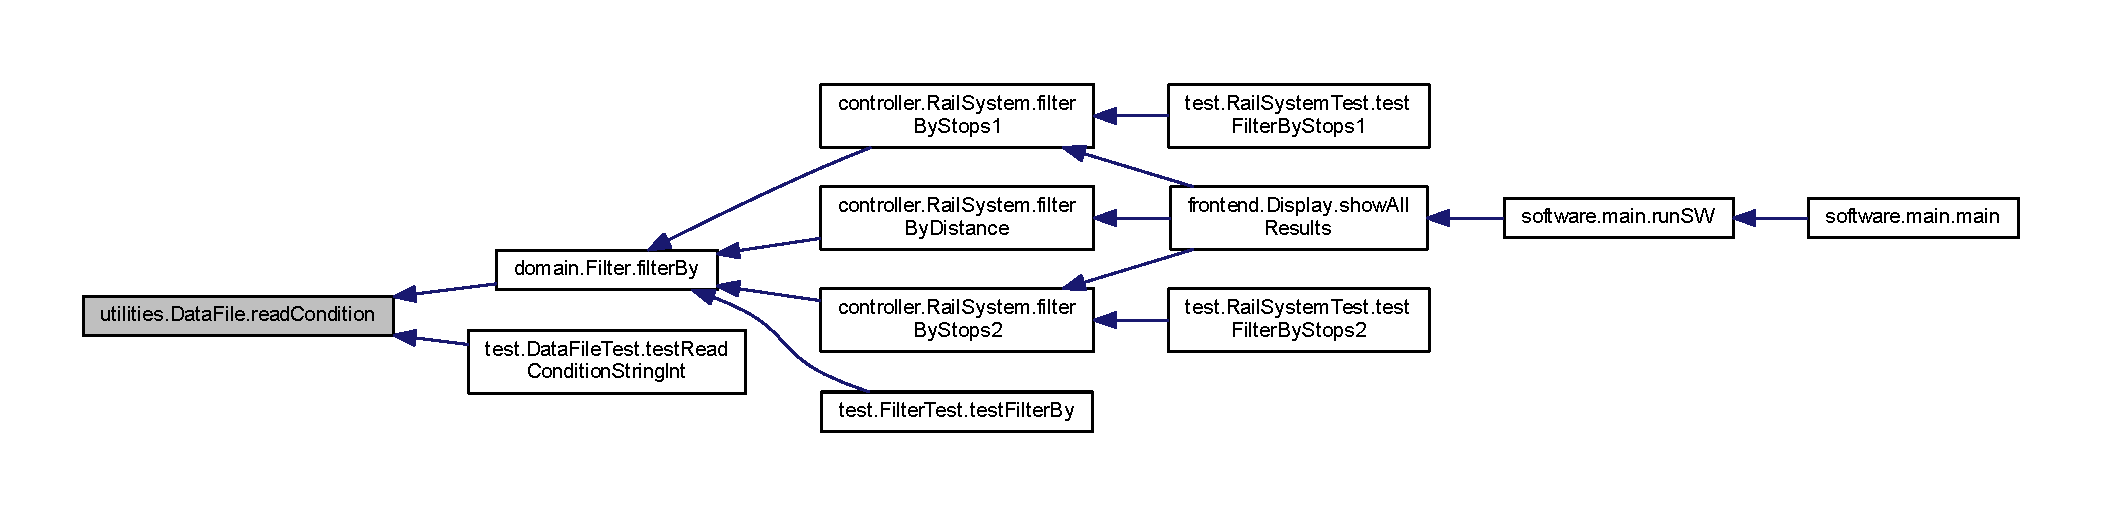
\includegraphics[width=350pt]{classutilities_1_1_data_file_ae44a128705ef07c67393153806fb5216_icgraph}
\end{center}
\end{figure}
\mbox{\Hypertarget{classutilities_1_1_data_file_aafa9fbee5003c8d9abcd0b02ba4b31dc}\label{classutilities_1_1_data_file_aafa9fbee5003c8d9abcd0b02ba4b31dc}} 
\index{utilities\+::\+Data\+File@{utilities\+::\+Data\+File}!read\+Double@{read\+Double}}
\index{read\+Double@{read\+Double}!utilities\+::\+Data\+File@{utilities\+::\+Data\+File}}
\subsubsection{\texorpdfstring{read\+Double()}{readDouble()}}
{\footnotesize\ttfamily static double utilities.\+Data\+File.\+read\+Double (\begin{DoxyParamCaption}\item[{\hyperlink{enumutilities_1_1_file_property}{File\+Property}}]{property,  }\item[{int}]{index\+\_\+filter }\end{DoxyParamCaption})\hspace{0.3cm}{\ttfamily [static]}}

Le um double do arquivo de entrada 
\begin{DoxyParams}{Parameters}
{\em property} & propriedade onde o double sera buscado \\
\hline
{\em index\+\_\+filter} & index identifica qual propriedade dentro do array que existe no arquivo \\
\hline
\end{DoxyParams}
\begin{DoxyReturn}{Returns}
retorna o double lido do arquivo 
\end{DoxyReturn}
Here is the call graph for this function\+:\nopagebreak
\begin{figure}[H]
\begin{center}
\leavevmode
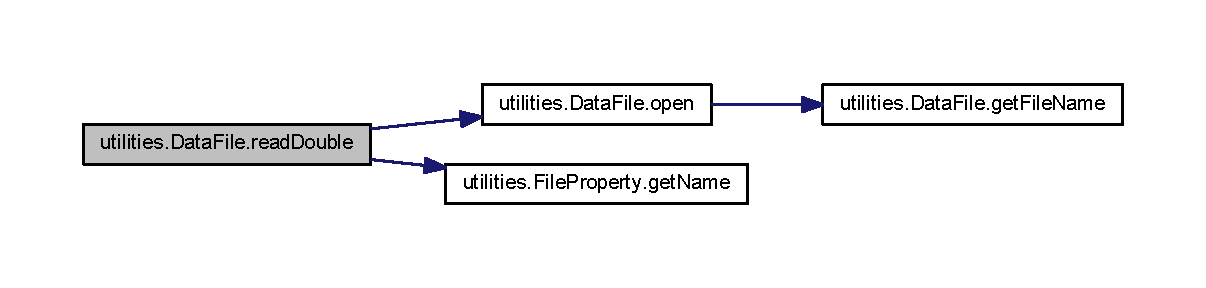
\includegraphics[width=350pt]{classutilities_1_1_data_file_aafa9fbee5003c8d9abcd0b02ba4b31dc_cgraph}
\end{center}
\end{figure}
Here is the caller graph for this function\+:\nopagebreak
\begin{figure}[H]
\begin{center}
\leavevmode
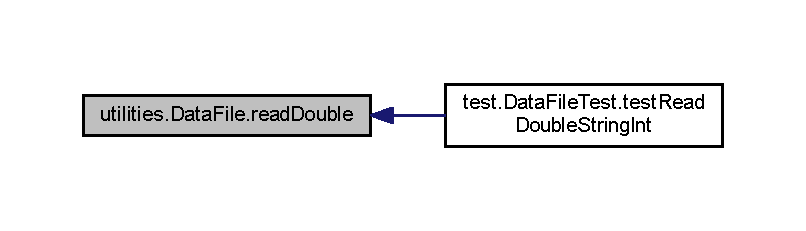
\includegraphics[width=350pt]{classutilities_1_1_data_file_aafa9fbee5003c8d9abcd0b02ba4b31dc_icgraph}
\end{center}
\end{figure}
\mbox{\Hypertarget{classutilities_1_1_data_file_a7576f90d40db372f262216f8f6a64c28}\label{classutilities_1_1_data_file_a7576f90d40db372f262216f8f6a64c28}} 
\index{utilities\+::\+Data\+File@{utilities\+::\+Data\+File}!read\+Integer@{read\+Integer}}
\index{read\+Integer@{read\+Integer}!utilities\+::\+Data\+File@{utilities\+::\+Data\+File}}
\subsubsection{\texorpdfstring{read\+Integer()}{readInteger()}}
{\footnotesize\ttfamily static int utilities.\+Data\+File.\+read\+Integer (\begin{DoxyParamCaption}\item[{\hyperlink{enumutilities_1_1_file_property}{File\+Property}}]{property,  }\item[{int}]{index\+\_\+filter }\end{DoxyParamCaption})\hspace{0.3cm}{\ttfamily [static]}}

Le um interiro do arquivo de entrada 
\begin{DoxyParams}{Parameters}
{\em property} & propriedade onde o inteiro sera buscado \\
\hline
{\em index\+\_\+filter} & index identifica qual propriedade dentro do array que existe no arquivo \\
\hline
\end{DoxyParams}
\begin{DoxyReturn}{Returns}
retorna o inteiro lido do arquivo 
\end{DoxyReturn}
Here is the call graph for this function\+:\nopagebreak
\begin{figure}[H]
\begin{center}
\leavevmode
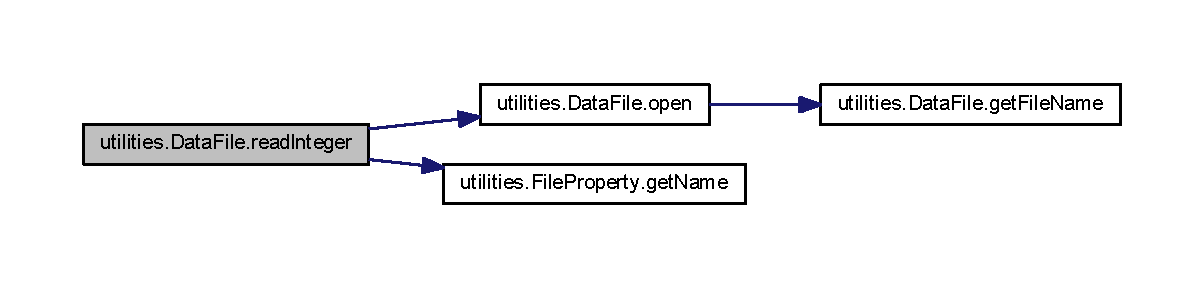
\includegraphics[width=350pt]{classutilities_1_1_data_file_a7576f90d40db372f262216f8f6a64c28_cgraph}
\end{center}
\end{figure}
Here is the caller graph for this function\+:\nopagebreak
\begin{figure}[H]
\begin{center}
\leavevmode
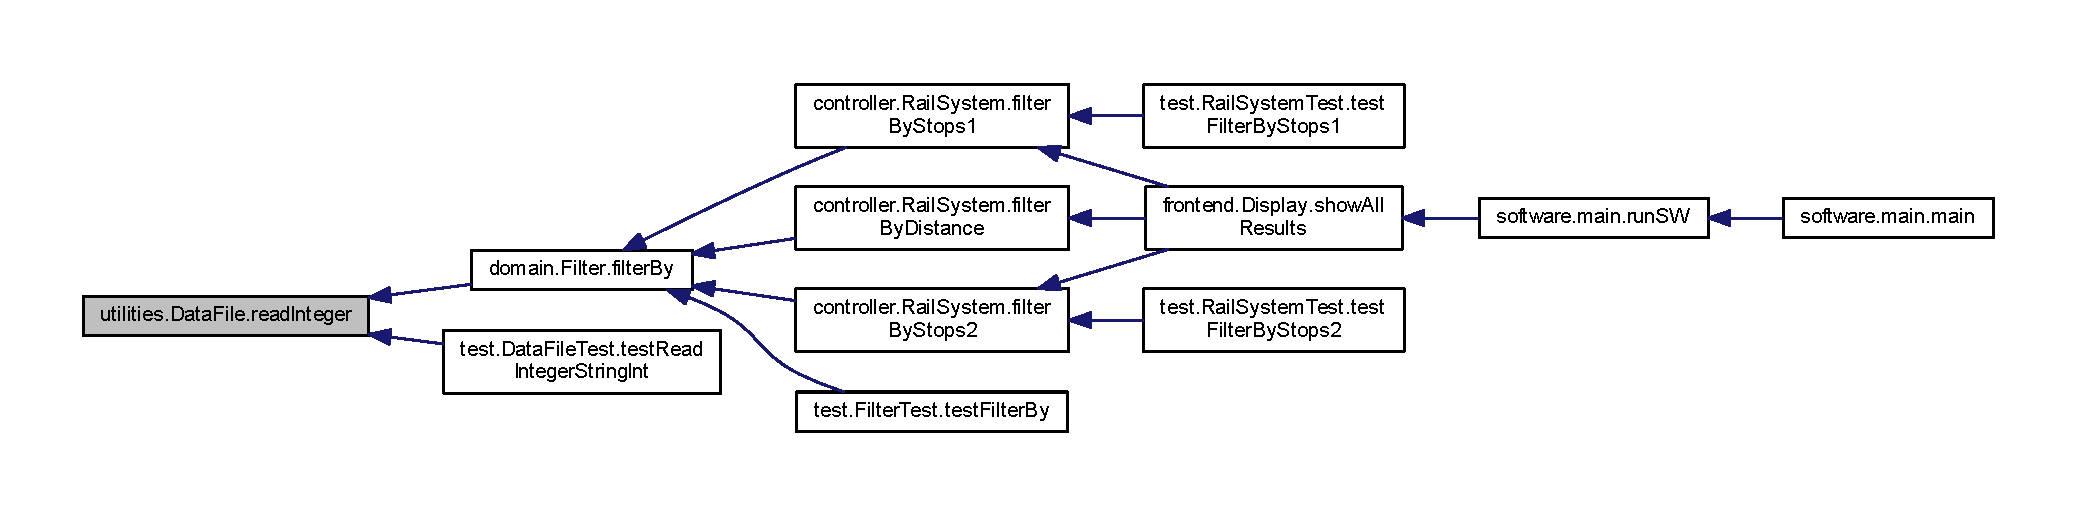
\includegraphics[width=350pt]{classutilities_1_1_data_file_a7576f90d40db372f262216f8f6a64c28_icgraph}
\end{center}
\end{figure}
\mbox{\Hypertarget{classutilities_1_1_data_file_a68332bb2b70bafbaae007d952ba4264b}\label{classutilities_1_1_data_file_a68332bb2b70bafbaae007d952ba4264b}} 
\index{utilities\+::\+Data\+File@{utilities\+::\+Data\+File}!read\+List@{read\+List}}
\index{read\+List@{read\+List}!utilities\+::\+Data\+File@{utilities\+::\+Data\+File}}
\subsubsection{\texorpdfstring{read\+List()}{readList()}\hspace{0.1cm}{\footnotesize\ttfamily [1/2]}}
{\footnotesize\ttfamily static String \mbox{[}$\,$\mbox{]} utilities.\+Data\+File.\+read\+List (\begin{DoxyParamCaption}\item[{\hyperlink{enumutilities_1_1_file_property}{File\+Property}}]{property }\end{DoxyParamCaption})\hspace{0.3cm}{\ttfamily [static]}}

Le uma lista de string do arquivo de entrada 
\begin{DoxyParams}{Parameters}
{\em property} & identificador da propriedade a ser lida \\
\hline
\end{DoxyParams}
\begin{DoxyReturn}{Returns}
retorna o array de string lido do arquivo 
\end{DoxyReturn}
Here is the caller graph for this function\+:\nopagebreak
\begin{figure}[H]
\begin{center}
\leavevmode
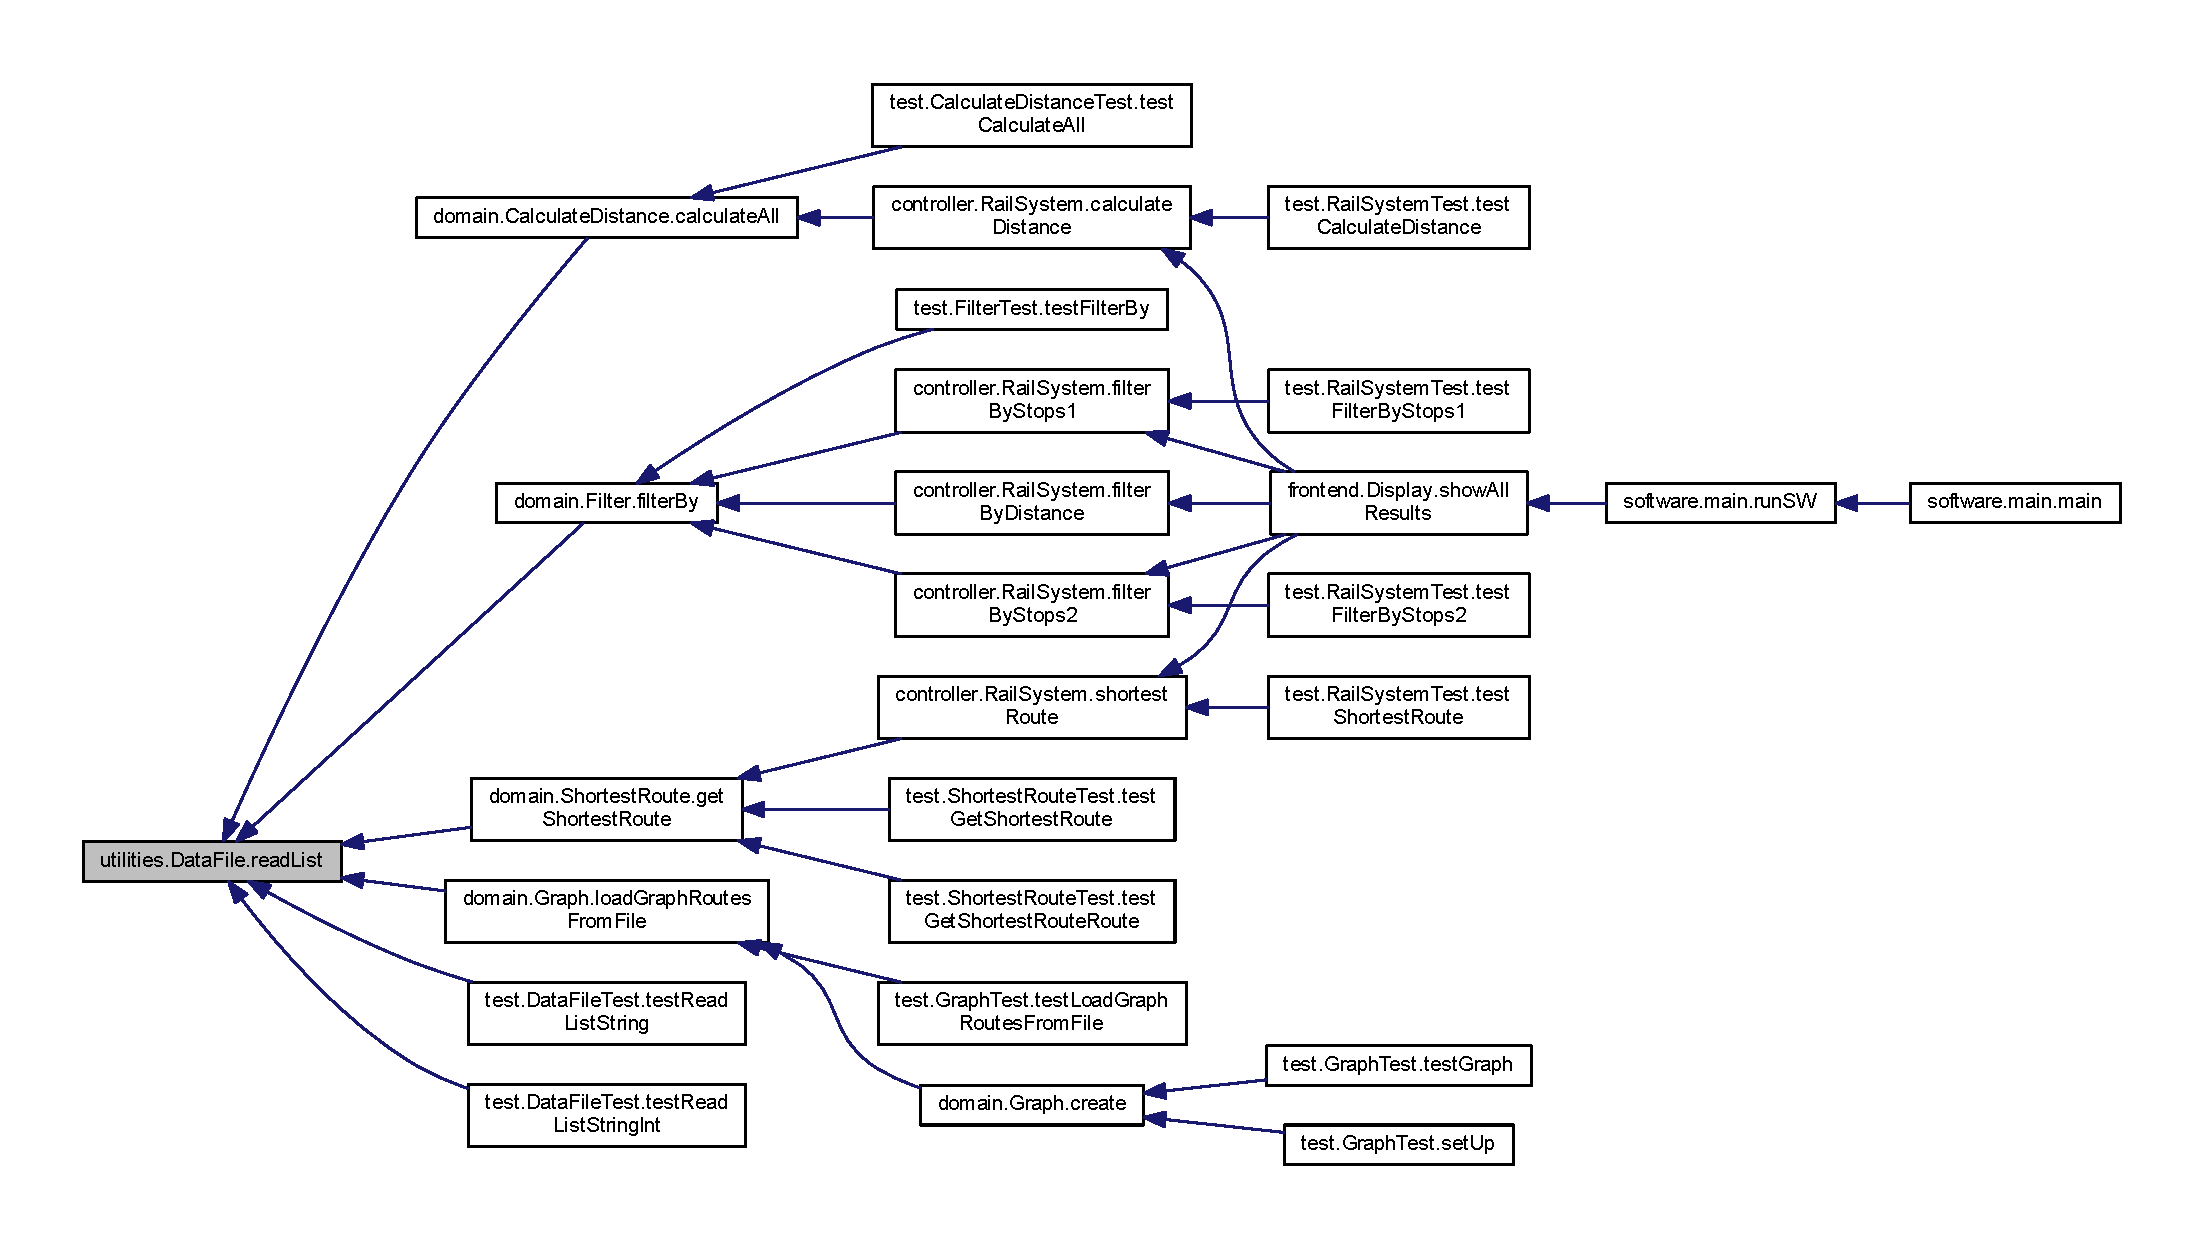
\includegraphics[width=350pt]{classutilities_1_1_data_file_a68332bb2b70bafbaae007d952ba4264b_icgraph}
\end{center}
\end{figure}
\mbox{\Hypertarget{classutilities_1_1_data_file_a86acc1699af206a96ab51c94d6663afe}\label{classutilities_1_1_data_file_a86acc1699af206a96ab51c94d6663afe}} 
\index{utilities\+::\+Data\+File@{utilities\+::\+Data\+File}!read\+List@{read\+List}}
\index{read\+List@{read\+List}!utilities\+::\+Data\+File@{utilities\+::\+Data\+File}}
\subsubsection{\texorpdfstring{read\+List()}{readList()}\hspace{0.1cm}{\footnotesize\ttfamily [2/2]}}
{\footnotesize\ttfamily static String \mbox{[}$\,$\mbox{]} utilities.\+Data\+File.\+read\+List (\begin{DoxyParamCaption}\item[{\hyperlink{enumutilities_1_1_file_property}{File\+Property}}]{property,  }\item[{int}]{index\+\_\+filter }\end{DoxyParamCaption})\hspace{0.3cm}{\ttfamily [static]}}

Le um array de string do arquivo de entrada 
\begin{DoxyParams}{Parameters}
{\em property} & propriedade onde o array de string sera buscado \\
\hline
{\em index\+\_\+filter} & index da propriedade a ser buscada ex\+: propriedade\mbox{[}index\mbox{]}.condition \\
\hline
\end{DoxyParams}
\begin{DoxyReturn}{Returns}
retorna o array de string lido do arquivo 
\end{DoxyReturn}
Here is the call graph for this function\+:\nopagebreak
\begin{figure}[H]
\begin{center}
\leavevmode
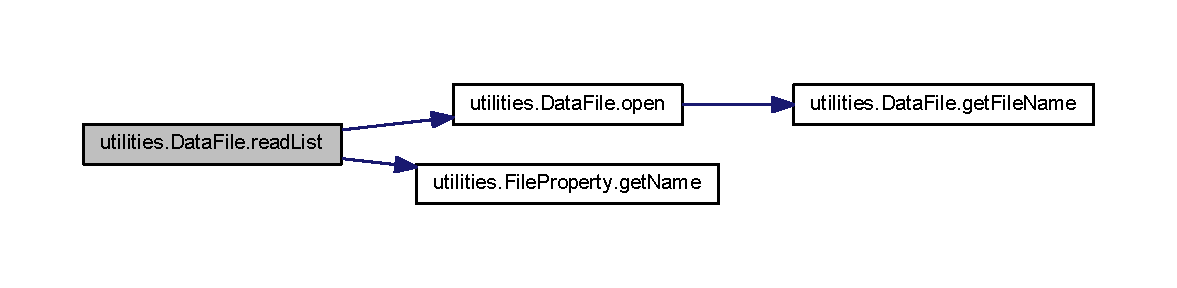
\includegraphics[width=350pt]{classutilities_1_1_data_file_a86acc1699af206a96ab51c94d6663afe_cgraph}
\end{center}
\end{figure}
\mbox{\Hypertarget{classutilities_1_1_data_file_adb4c1c9272d3497615385f4f8278ab60}\label{classutilities_1_1_data_file_adb4c1c9272d3497615385f4f8278ab60}} 
\index{utilities\+::\+Data\+File@{utilities\+::\+Data\+File}!read\+Literal\+Operand@{read\+Literal\+Operand}}
\index{read\+Literal\+Operand@{read\+Literal\+Operand}!utilities\+::\+Data\+File@{utilities\+::\+Data\+File}}
\subsubsection{\texorpdfstring{read\+Literal\+Operand()}{readLiteralOperand()}}
{\footnotesize\ttfamily static String utilities.\+Data\+File.\+read\+Literal\+Operand (\begin{DoxyParamCaption}\item[{\hyperlink{enumutilities_1_1_file_property}{File\+Property}}]{property,  }\item[{int}]{index\+\_\+filter }\end{DoxyParamCaption})\hspace{0.3cm}{\ttfamily [static]}}

Le um operando na forma literal do arquivo de entrada


\begin{DoxyParams}{Parameters}
{\em property} & propriedade a ser lida \\
\hline
\end{DoxyParams}
\begin{DoxyReturn}{Returns}
retorna o operando, na forma literal, lido do arquivo 
\end{DoxyReturn}

\begin{DoxyParams}{Parameters}
{\em index\+\_\+filter} & index identifica qual propriedade dentro do array que existe no arquivo \\
\hline
\end{DoxyParams}
\begin{DoxyReturn}{Returns}
retorna o operando, na forma literal, lido do arquivo 
\end{DoxyReturn}
Here is the call graph for this function\+:\nopagebreak
\begin{figure}[H]
\begin{center}
\leavevmode
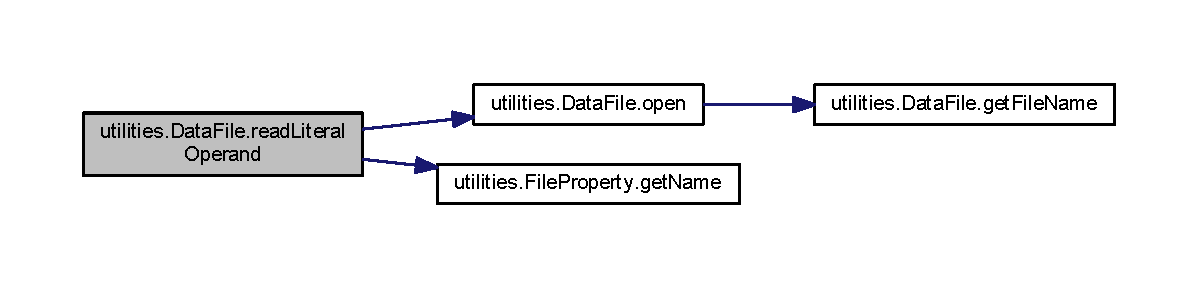
\includegraphics[width=350pt]{classutilities_1_1_data_file_adb4c1c9272d3497615385f4f8278ab60_cgraph}
\end{center}
\end{figure}
Here is the caller graph for this function\+:\nopagebreak
\begin{figure}[H]
\begin{center}
\leavevmode
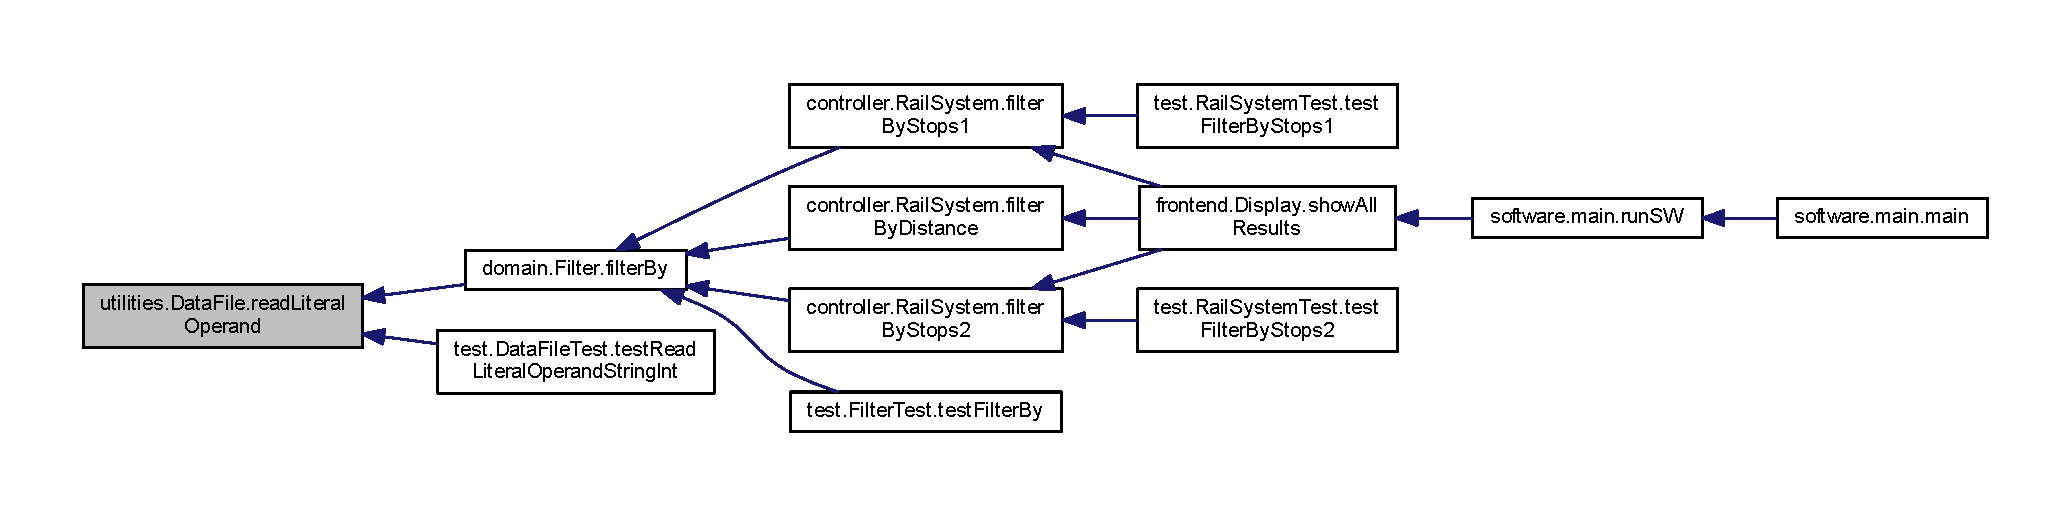
\includegraphics[width=350pt]{classutilities_1_1_data_file_adb4c1c9272d3497615385f4f8278ab60_icgraph}
\end{center}
\end{figure}
\mbox{\Hypertarget{classutilities_1_1_data_file_a03d4af9888db5dfd5031fd3ead4964bf}\label{classutilities_1_1_data_file_a03d4af9888db5dfd5031fd3ead4964bf}} 
\index{utilities\+::\+Data\+File@{utilities\+::\+Data\+File}!set\+File\+Name@{set\+File\+Name}}
\index{set\+File\+Name@{set\+File\+Name}!utilities\+::\+Data\+File@{utilities\+::\+Data\+File}}
\subsubsection{\texorpdfstring{set\+File\+Name()}{setFileName()}}
{\footnotesize\ttfamily static void utilities.\+Data\+File.\+set\+File\+Name (\begin{DoxyParamCaption}\item[{String}]{file }\end{DoxyParamCaption})\hspace{0.3cm}{\ttfamily [static]}}

Configura o nome do arquivo


\begin{DoxyParams}{Parameters}
{\em file} & path + nome do arquivo a ser utilizado para entrada dos valores \\
\hline
\end{DoxyParams}
Here is the call graph for this function\+:\nopagebreak
\begin{figure}[H]
\begin{center}
\leavevmode
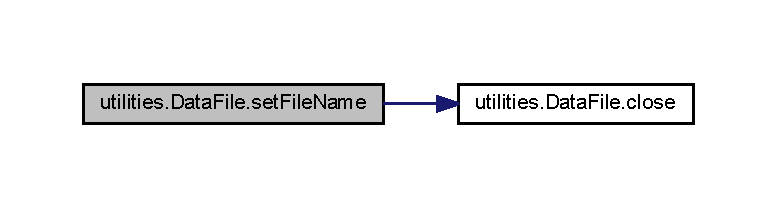
\includegraphics[width=350pt]{classutilities_1_1_data_file_a03d4af9888db5dfd5031fd3ead4964bf_cgraph}
\end{center}
\end{figure}
Here is the caller graph for this function\+:\nopagebreak
\begin{figure}[H]
\begin{center}
\leavevmode
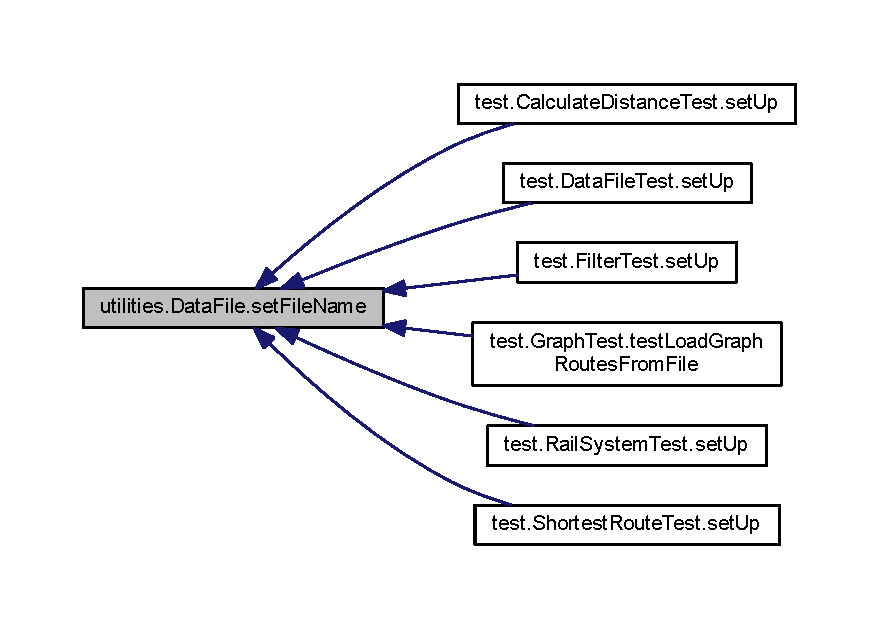
\includegraphics[width=350pt]{classutilities_1_1_data_file_a03d4af9888db5dfd5031fd3ead4964bf_icgraph}
\end{center}
\end{figure}


\subsection{Member Data Documentation}
\mbox{\Hypertarget{classutilities_1_1_data_file_a7db48e719d69b2fb08dec6730949acf9}\label{classutilities_1_1_data_file_a7db48e719d69b2fb08dec6730949acf9}} 
\index{utilities\+::\+Data\+File@{utilities\+::\+Data\+File}!D\+I\+S\+T\+A\+N\+C\+E\+\_\+\+C\+O\+N\+D\+I\+T\+I\+ON@{D\+I\+S\+T\+A\+N\+C\+E\+\_\+\+C\+O\+N\+D\+I\+T\+I\+ON}}
\index{D\+I\+S\+T\+A\+N\+C\+E\+\_\+\+C\+O\+N\+D\+I\+T\+I\+ON@{D\+I\+S\+T\+A\+N\+C\+E\+\_\+\+C\+O\+N\+D\+I\+T\+I\+ON}!utilities\+::\+Data\+File@{utilities\+::\+Data\+File}}
\subsubsection{\texorpdfstring{D\+I\+S\+T\+A\+N\+C\+E\+\_\+\+C\+O\+N\+D\+I\+T\+I\+ON}{DISTANCE\_CONDITION}}
{\footnotesize\ttfamily final int utilities.\+Data\+File.\+D\+I\+S\+T\+A\+N\+C\+E\+\_\+\+C\+O\+N\+D\+I\+T\+I\+ON =3\hspace{0.3cm}{\ttfamily [static]}}

\mbox{\Hypertarget{classutilities_1_1_data_file_acc01b0a1464087e54962b7c6202dbb5f}\label{classutilities_1_1_data_file_acc01b0a1464087e54962b7c6202dbb5f}} 
\index{utilities\+::\+Data\+File@{utilities\+::\+Data\+File}!file\+\_\+name@{file\+\_\+name}}
\index{file\+\_\+name@{file\+\_\+name}!utilities\+::\+Data\+File@{utilities\+::\+Data\+File}}
\subsubsection{\texorpdfstring{file\+\_\+name}{file\_name}}
{\footnotesize\ttfamily String utilities.\+Data\+File.\+file\+\_\+name = \hyperlink{classutilities_1_1_data_file_ab2cdae484f28934cf77316bbf9af0b72}{P\+A\+T\+H\+\_\+\+F\+I\+LE}\hspace{0.3cm}{\ttfamily [static]}, {\ttfamily [private]}}

\mbox{\Hypertarget{classutilities_1_1_data_file_a6d7f06ae7db77b3b202c31190c2281e3}\label{classutilities_1_1_data_file_a6d7f06ae7db77b3b202c31190c2281e3}} 
\index{utilities\+::\+Data\+File@{utilities\+::\+Data\+File}!F\+I\+L\+E\+\_\+\+T\+E\+S\+T\+S\+\_\+\+C\+A\+S\+ES@{F\+I\+L\+E\+\_\+\+T\+E\+S\+T\+S\+\_\+\+C\+A\+S\+ES}}
\index{F\+I\+L\+E\+\_\+\+T\+E\+S\+T\+S\+\_\+\+C\+A\+S\+ES@{F\+I\+L\+E\+\_\+\+T\+E\+S\+T\+S\+\_\+\+C\+A\+S\+ES}!utilities\+::\+Data\+File@{utilities\+::\+Data\+File}}
\subsubsection{\texorpdfstring{F\+I\+L\+E\+\_\+\+T\+E\+S\+T\+S\+\_\+\+C\+A\+S\+ES}{FILE\_TESTS\_CASES}}
{\footnotesize\ttfamily final String utilities.\+Data\+File.\+F\+I\+L\+E\+\_\+\+T\+E\+S\+T\+S\+\_\+\+C\+A\+S\+ES = \char`\"{}F\+I\+L\+E\+\_\+\+T\+E\+S\+T\+\_\+\+C\+A\+S\+E.\+txt\char`\"{}\hspace{0.3cm}{\ttfamily [static]}}

\mbox{\Hypertarget{classutilities_1_1_data_file_a80202aa4edd480f4404d9fd4adcedbfc}\label{classutilities_1_1_data_file_a80202aa4edd480f4404d9fd4adcedbfc}} 
\index{utilities\+::\+Data\+File@{utilities\+::\+Data\+File}!input@{input}}
\index{input@{input}!utilities\+::\+Data\+File@{utilities\+::\+Data\+File}}
\subsubsection{\texorpdfstring{input}{input}}
{\footnotesize\ttfamily Input\+Stream utilities.\+Data\+File.\+input = null\hspace{0.3cm}{\ttfamily [static]}, {\ttfamily [package]}}

\mbox{\Hypertarget{classutilities_1_1_data_file_ab2cdae484f28934cf77316bbf9af0b72}\label{classutilities_1_1_data_file_ab2cdae484f28934cf77316bbf9af0b72}} 
\index{utilities\+::\+Data\+File@{utilities\+::\+Data\+File}!P\+A\+T\+H\+\_\+\+F\+I\+LE@{P\+A\+T\+H\+\_\+\+F\+I\+LE}}
\index{P\+A\+T\+H\+\_\+\+F\+I\+LE@{P\+A\+T\+H\+\_\+\+F\+I\+LE}!utilities\+::\+Data\+File@{utilities\+::\+Data\+File}}
\subsubsection{\texorpdfstring{P\+A\+T\+H\+\_\+\+F\+I\+LE}{PATH\_FILE}}
{\footnotesize\ttfamily final String utilities.\+Data\+File.\+P\+A\+T\+H\+\_\+\+F\+I\+LE = \char`\"{}input.\+txt\char`\"{}\hspace{0.3cm}{\ttfamily [static]}}

Nome do Arquivo de entrada \mbox{\Hypertarget{classutilities_1_1_data_file_aee831317a6c670d621683dbfadf1d19f}\label{classutilities_1_1_data_file_aee831317a6c670d621683dbfadf1d19f}} 
\index{utilities\+::\+Data\+File@{utilities\+::\+Data\+File}!P\+A\+T\+T\+E\+R\+N\+\_\+\+C\+O\+N\+D\+I\+T\+I\+ON@{P\+A\+T\+T\+E\+R\+N\+\_\+\+C\+O\+N\+D\+I\+T\+I\+ON}}
\index{P\+A\+T\+T\+E\+R\+N\+\_\+\+C\+O\+N\+D\+I\+T\+I\+ON@{P\+A\+T\+T\+E\+R\+N\+\_\+\+C\+O\+N\+D\+I\+T\+I\+ON}!utilities\+::\+Data\+File@{utilities\+::\+Data\+File}}
\subsubsection{\texorpdfstring{P\+A\+T\+T\+E\+R\+N\+\_\+\+C\+O\+N\+D\+I\+T\+I\+ON}{PATTERN\_CONDITION}}
{\footnotesize\ttfamily final String utilities.\+Data\+File.\+P\+A\+T\+T\+E\+R\+N\+\_\+\+C\+O\+N\+D\+I\+T\+I\+ON =\char`\"{}\mbox{[}$^\wedge$$<$$>$=!\mbox{]}\char`\"{}\hspace{0.3cm}{\ttfamily [static]}, {\ttfamily [private]}}

\mbox{\Hypertarget{classutilities_1_1_data_file_ac00c547e129cb9c057f7a0d499015797}\label{classutilities_1_1_data_file_ac00c547e129cb9c057f7a0d499015797}} 
\index{utilities\+::\+Data\+File@{utilities\+::\+Data\+File}!P\+A\+T\+T\+E\+R\+N\+\_\+\+D\+O\+U\+B\+LE@{P\+A\+T\+T\+E\+R\+N\+\_\+\+D\+O\+U\+B\+LE}}
\index{P\+A\+T\+T\+E\+R\+N\+\_\+\+D\+O\+U\+B\+LE@{P\+A\+T\+T\+E\+R\+N\+\_\+\+D\+O\+U\+B\+LE}!utilities\+::\+Data\+File@{utilities\+::\+Data\+File}}
\subsubsection{\texorpdfstring{P\+A\+T\+T\+E\+R\+N\+\_\+\+D\+O\+U\+B\+LE}{PATTERN\_DOUBLE}}
{\footnotesize\ttfamily final String utilities.\+Data\+File.\+P\+A\+T\+T\+E\+R\+N\+\_\+\+D\+O\+U\+B\+LE =\char`\"{}\mbox{[}$^\wedge$0-\/9.,\mbox{]}\char`\"{}\hspace{0.3cm}{\ttfamily [static]}, {\ttfamily [private]}}

\mbox{\Hypertarget{classutilities_1_1_data_file_a51e037b86bf7cd4b6ce02a384d9ad6f2}\label{classutilities_1_1_data_file_a51e037b86bf7cd4b6ce02a384d9ad6f2}} 
\index{utilities\+::\+Data\+File@{utilities\+::\+Data\+File}!P\+A\+T\+T\+E\+R\+N\+\_\+\+I\+N\+T\+E\+G\+ER@{P\+A\+T\+T\+E\+R\+N\+\_\+\+I\+N\+T\+E\+G\+ER}}
\index{P\+A\+T\+T\+E\+R\+N\+\_\+\+I\+N\+T\+E\+G\+ER@{P\+A\+T\+T\+E\+R\+N\+\_\+\+I\+N\+T\+E\+G\+ER}!utilities\+::\+Data\+File@{utilities\+::\+Data\+File}}
\subsubsection{\texorpdfstring{P\+A\+T\+T\+E\+R\+N\+\_\+\+I\+N\+T\+E\+G\+ER}{PATTERN\_INTEGER}}
{\footnotesize\ttfamily final String utilities.\+Data\+File.\+P\+A\+T\+T\+E\+R\+N\+\_\+\+I\+N\+T\+E\+G\+ER =\char`\"{}\mbox{[}$^\wedge$0-\/9\mbox{]}\char`\"{}\hspace{0.3cm}{\ttfamily [static]}, {\ttfamily [private]}}

\mbox{\Hypertarget{classutilities_1_1_data_file_a25b4360923bcdd2e38e81df53297ee94}\label{classutilities_1_1_data_file_a25b4360923bcdd2e38e81df53297ee94}} 
\index{utilities\+::\+Data\+File@{utilities\+::\+Data\+File}!P\+A\+T\+T\+E\+R\+N\+\_\+\+L\+I\+ST@{P\+A\+T\+T\+E\+R\+N\+\_\+\+L\+I\+ST}}
\index{P\+A\+T\+T\+E\+R\+N\+\_\+\+L\+I\+ST@{P\+A\+T\+T\+E\+R\+N\+\_\+\+L\+I\+ST}!utilities\+::\+Data\+File@{utilities\+::\+Data\+File}}
\subsubsection{\texorpdfstring{P\+A\+T\+T\+E\+R\+N\+\_\+\+L\+I\+ST}{PATTERN\_LIST}}
{\footnotesize\ttfamily final String utilities.\+Data\+File.\+P\+A\+T\+T\+E\+R\+N\+\_\+\+L\+I\+ST =\char`\"{}\mbox{[}$^\wedge$a-\/zA-\/Z0-\/9.,\mbox{]}\char`\"{}\hspace{0.3cm}{\ttfamily [static]}, {\ttfamily [private]}}

\mbox{\Hypertarget{classutilities_1_1_data_file_aeb2abc62f5fe561e1425331c49c1a58d}\label{classutilities_1_1_data_file_aeb2abc62f5fe561e1425331c49c1a58d}} 
\index{utilities\+::\+Data\+File@{utilities\+::\+Data\+File}!P\+A\+T\+T\+E\+R\+N\+\_\+\+O\+P\+E\+R\+A\+ND@{P\+A\+T\+T\+E\+R\+N\+\_\+\+O\+P\+E\+R\+A\+ND}}
\index{P\+A\+T\+T\+E\+R\+N\+\_\+\+O\+P\+E\+R\+A\+ND@{P\+A\+T\+T\+E\+R\+N\+\_\+\+O\+P\+E\+R\+A\+ND}!utilities\+::\+Data\+File@{utilities\+::\+Data\+File}}
\subsubsection{\texorpdfstring{P\+A\+T\+T\+E\+R\+N\+\_\+\+O\+P\+E\+R\+A\+ND}{PATTERN\_OPERAND}}
{\footnotesize\ttfamily final String utilities.\+Data\+File.\+P\+A\+T\+T\+E\+R\+N\+\_\+\+O\+P\+E\+R\+A\+ND =\char`\"{}\mbox{[}$^\wedge$a-\/zA-\/Z,\mbox{]}\char`\"{}\hspace{0.3cm}{\ttfamily [static]}, {\ttfamily [private]}}

\mbox{\Hypertarget{classutilities_1_1_data_file_a56e3023d87523528a6126799b02b089d}\label{classutilities_1_1_data_file_a56e3023d87523528a6126799b02b089d}} 
\index{utilities\+::\+Data\+File@{utilities\+::\+Data\+File}!prop@{prop}}
\index{prop@{prop}!utilities\+::\+Data\+File@{utilities\+::\+Data\+File}}
\subsubsection{\texorpdfstring{prop}{prop}}
{\footnotesize\ttfamily Properties utilities.\+Data\+File.\+prop = new Properties()\hspace{0.3cm}{\ttfamily [static]}, {\ttfamily [package]}}

\mbox{\Hypertarget{classutilities_1_1_data_file_ae7a89abc44a0f02d5b6205b6e2f53a06}\label{classutilities_1_1_data_file_ae7a89abc44a0f02d5b6205b6e2f53a06}} 
\index{utilities\+::\+Data\+File@{utilities\+::\+Data\+File}!S\+E\+P\+A\+R\+A\+T\+OR@{S\+E\+P\+A\+R\+A\+T\+OR}}
\index{S\+E\+P\+A\+R\+A\+T\+OR@{S\+E\+P\+A\+R\+A\+T\+OR}!utilities\+::\+Data\+File@{utilities\+::\+Data\+File}}
\subsubsection{\texorpdfstring{S\+E\+P\+A\+R\+A\+T\+OR}{SEPARATOR}}
{\footnotesize\ttfamily final String utilities.\+Data\+File.\+S\+E\+P\+A\+R\+A\+T\+OR =\char`\"{},\char`\"{}\hspace{0.3cm}{\ttfamily [static]}, {\ttfamily [private]}}

\mbox{\Hypertarget{classutilities_1_1_data_file_a73169a0777ef2c7e224420ab3f4be9dc}\label{classutilities_1_1_data_file_a73169a0777ef2c7e224420ab3f4be9dc}} 
\index{utilities\+::\+Data\+File@{utilities\+::\+Data\+File}!S\+T\+O\+P1\+\_\+\+C\+O\+N\+D\+I\+T\+I\+ON@{S\+T\+O\+P1\+\_\+\+C\+O\+N\+D\+I\+T\+I\+ON}}
\index{S\+T\+O\+P1\+\_\+\+C\+O\+N\+D\+I\+T\+I\+ON@{S\+T\+O\+P1\+\_\+\+C\+O\+N\+D\+I\+T\+I\+ON}!utilities\+::\+Data\+File@{utilities\+::\+Data\+File}}
\subsubsection{\texorpdfstring{S\+T\+O\+P1\+\_\+\+C\+O\+N\+D\+I\+T\+I\+ON}{STOP1\_CONDITION}}
{\footnotesize\ttfamily final int utilities.\+Data\+File.\+S\+T\+O\+P1\+\_\+\+C\+O\+N\+D\+I\+T\+I\+ON =1\hspace{0.3cm}{\ttfamily [static]}}

\mbox{\Hypertarget{classutilities_1_1_data_file_afdb877fcbb93d5bf2e6757f844c0a0e0}\label{classutilities_1_1_data_file_afdb877fcbb93d5bf2e6757f844c0a0e0}} 
\index{utilities\+::\+Data\+File@{utilities\+::\+Data\+File}!S\+T\+O\+P2\+\_\+\+C\+O\+N\+D\+I\+T\+I\+ON@{S\+T\+O\+P2\+\_\+\+C\+O\+N\+D\+I\+T\+I\+ON}}
\index{S\+T\+O\+P2\+\_\+\+C\+O\+N\+D\+I\+T\+I\+ON@{S\+T\+O\+P2\+\_\+\+C\+O\+N\+D\+I\+T\+I\+ON}!utilities\+::\+Data\+File@{utilities\+::\+Data\+File}}
\subsubsection{\texorpdfstring{S\+T\+O\+P2\+\_\+\+C\+O\+N\+D\+I\+T\+I\+ON}{STOP2\_CONDITION}}
{\footnotesize\ttfamily final int utilities.\+Data\+File.\+S\+T\+O\+P2\+\_\+\+C\+O\+N\+D\+I\+T\+I\+ON =2\hspace{0.3cm}{\ttfamily [static]}}



The documentation for this class was generated from the following file\+:\begin{DoxyCompactItemize}
\item 
D\+:/workspace/\+Train\+Vagas/src/utilities/\hyperlink{_data_file_8java}{Data\+File.\+java}\end{DoxyCompactItemize}

\hypertarget{classtest_1_1_data_file_test}{}\section{test.\+Data\+File\+Test Class Reference}
\label{classtest_1_1_data_file_test}\index{test.\+Data\+File\+Test@{test.\+Data\+File\+Test}}
\subsection*{Public Member Functions}
\begin{DoxyCompactItemize}
\item 
void \hyperlink{classtest_1_1_data_file_test_a0c4aa82f4822e250fa2ea1d238f25f87}{set\+Up} ()  throws Exception 
\item 
void \hyperlink{classtest_1_1_data_file_test_aa7338ead543ecd8b09f2a0d5a93c3ee8}{test\+Open} ()
\item 
void \hyperlink{classtest_1_1_data_file_test_ad4b0d957eebabf51055d0e7c8be254e7}{test\+Read\+List\+String} ()
\item 
void \hyperlink{classtest_1_1_data_file_test_ab61a29d98e2d1b08099008e0a5c53b63}{test\+Read\+List\+String\+Int} ()
\item 
void \hyperlink{classtest_1_1_data_file_test_afceb03fbe887feb7c9c51074ea1c41d8}{test\+Read\+Condition\+String\+Int} ()
\item 
void \hyperlink{classtest_1_1_data_file_test_a839677c199693ab93375ec09dfbb3407}{test\+Read\+Double\+String\+Int} ()
\item 
void \hyperlink{classtest_1_1_data_file_test_aa614885277711640980410c5faa5b609}{test\+Read\+Integer\+String\+Int} ()
\item 
void \hyperlink{classtest_1_1_data_file_test_ad4298b1da8ab563a46e4adfdc3d15720}{test\+Read\+Literal\+Operand\+String\+Int} ()
\end{DoxyCompactItemize}


\subsection{Member Function Documentation}
\mbox{\Hypertarget{classtest_1_1_data_file_test_a0c4aa82f4822e250fa2ea1d238f25f87}\label{classtest_1_1_data_file_test_a0c4aa82f4822e250fa2ea1d238f25f87}} 
\index{test\+::\+Data\+File\+Test@{test\+::\+Data\+File\+Test}!set\+Up@{set\+Up}}
\index{set\+Up@{set\+Up}!test\+::\+Data\+File\+Test@{test\+::\+Data\+File\+Test}}
\subsubsection{\texorpdfstring{set\+Up()}{setUp()}}
{\footnotesize\ttfamily void test.\+Data\+File\+Test.\+set\+Up (\begin{DoxyParamCaption}{ }\end{DoxyParamCaption}) throws Exception}

Here is the call graph for this function\+:\nopagebreak
\begin{figure}[H]
\begin{center}
\leavevmode
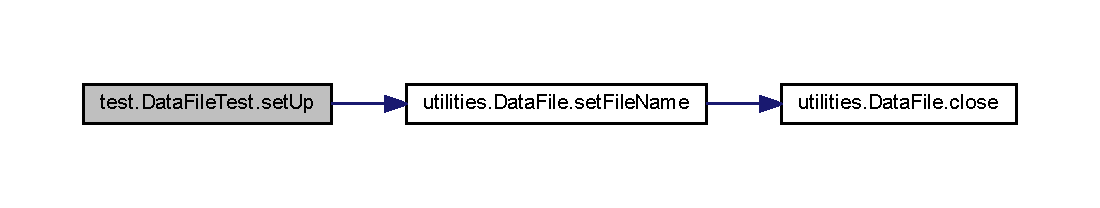
\includegraphics[width=350pt]{classtest_1_1_data_file_test_a0c4aa82f4822e250fa2ea1d238f25f87_cgraph}
\end{center}
\end{figure}
\mbox{\Hypertarget{classtest_1_1_data_file_test_aa7338ead543ecd8b09f2a0d5a93c3ee8}\label{classtest_1_1_data_file_test_aa7338ead543ecd8b09f2a0d5a93c3ee8}} 
\index{test\+::\+Data\+File\+Test@{test\+::\+Data\+File\+Test}!test\+Open@{test\+Open}}
\index{test\+Open@{test\+Open}!test\+::\+Data\+File\+Test@{test\+::\+Data\+File\+Test}}
\subsubsection{\texorpdfstring{test\+Open()}{testOpen()}}
{\footnotesize\ttfamily void test.\+Data\+File\+Test.\+test\+Open (\begin{DoxyParamCaption}{ }\end{DoxyParamCaption})}

Here is the call graph for this function\+:\nopagebreak
\begin{figure}[H]
\begin{center}
\leavevmode
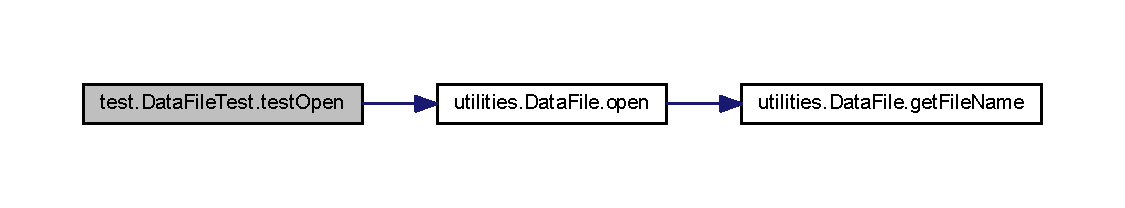
\includegraphics[width=350pt]{classtest_1_1_data_file_test_aa7338ead543ecd8b09f2a0d5a93c3ee8_cgraph}
\end{center}
\end{figure}
\mbox{\Hypertarget{classtest_1_1_data_file_test_afceb03fbe887feb7c9c51074ea1c41d8}\label{classtest_1_1_data_file_test_afceb03fbe887feb7c9c51074ea1c41d8}} 
\index{test\+::\+Data\+File\+Test@{test\+::\+Data\+File\+Test}!test\+Read\+Condition\+String\+Int@{test\+Read\+Condition\+String\+Int}}
\index{test\+Read\+Condition\+String\+Int@{test\+Read\+Condition\+String\+Int}!test\+::\+Data\+File\+Test@{test\+::\+Data\+File\+Test}}
\subsubsection{\texorpdfstring{test\+Read\+Condition\+String\+Int()}{testReadConditionStringInt()}}
{\footnotesize\ttfamily void test.\+Data\+File\+Test.\+test\+Read\+Condition\+String\+Int (\begin{DoxyParamCaption}{ }\end{DoxyParamCaption})}

Here is the call graph for this function\+:\nopagebreak
\begin{figure}[H]
\begin{center}
\leavevmode
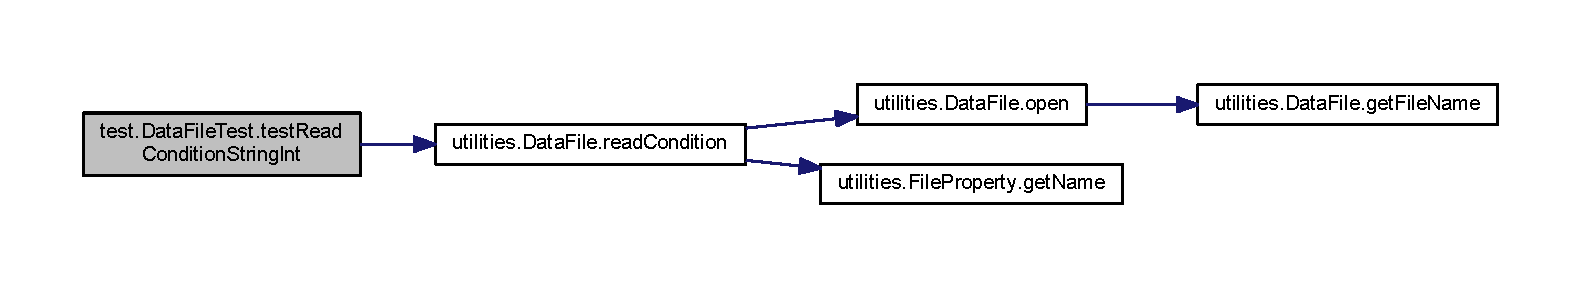
\includegraphics[width=350pt]{classtest_1_1_data_file_test_afceb03fbe887feb7c9c51074ea1c41d8_cgraph}
\end{center}
\end{figure}
\mbox{\Hypertarget{classtest_1_1_data_file_test_a839677c199693ab93375ec09dfbb3407}\label{classtest_1_1_data_file_test_a839677c199693ab93375ec09dfbb3407}} 
\index{test\+::\+Data\+File\+Test@{test\+::\+Data\+File\+Test}!test\+Read\+Double\+String\+Int@{test\+Read\+Double\+String\+Int}}
\index{test\+Read\+Double\+String\+Int@{test\+Read\+Double\+String\+Int}!test\+::\+Data\+File\+Test@{test\+::\+Data\+File\+Test}}
\subsubsection{\texorpdfstring{test\+Read\+Double\+String\+Int()}{testReadDoubleStringInt()}}
{\footnotesize\ttfamily void test.\+Data\+File\+Test.\+test\+Read\+Double\+String\+Int (\begin{DoxyParamCaption}{ }\end{DoxyParamCaption})}

Here is the call graph for this function\+:\nopagebreak
\begin{figure}[H]
\begin{center}
\leavevmode
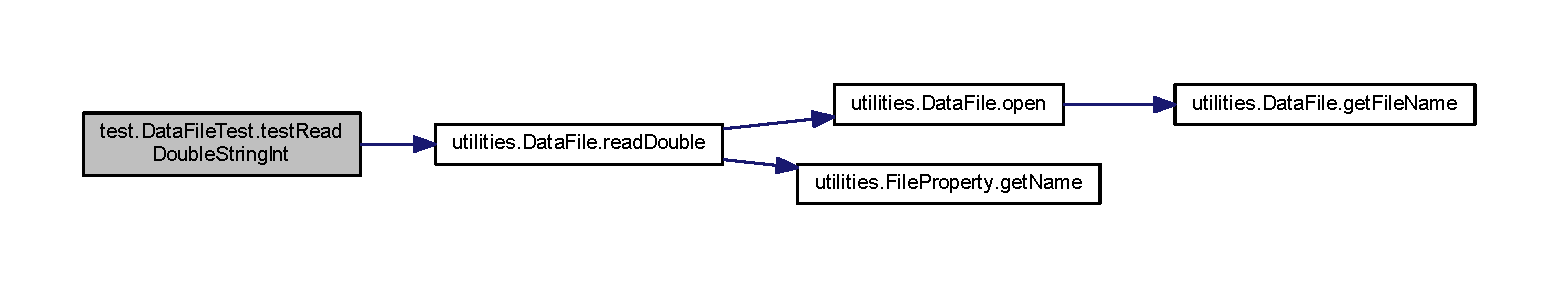
\includegraphics[width=350pt]{classtest_1_1_data_file_test_a839677c199693ab93375ec09dfbb3407_cgraph}
\end{center}
\end{figure}
\mbox{\Hypertarget{classtest_1_1_data_file_test_aa614885277711640980410c5faa5b609}\label{classtest_1_1_data_file_test_aa614885277711640980410c5faa5b609}} 
\index{test\+::\+Data\+File\+Test@{test\+::\+Data\+File\+Test}!test\+Read\+Integer\+String\+Int@{test\+Read\+Integer\+String\+Int}}
\index{test\+Read\+Integer\+String\+Int@{test\+Read\+Integer\+String\+Int}!test\+::\+Data\+File\+Test@{test\+::\+Data\+File\+Test}}
\subsubsection{\texorpdfstring{test\+Read\+Integer\+String\+Int()}{testReadIntegerStringInt()}}
{\footnotesize\ttfamily void test.\+Data\+File\+Test.\+test\+Read\+Integer\+String\+Int (\begin{DoxyParamCaption}{ }\end{DoxyParamCaption})}

Here is the call graph for this function\+:\nopagebreak
\begin{figure}[H]
\begin{center}
\leavevmode
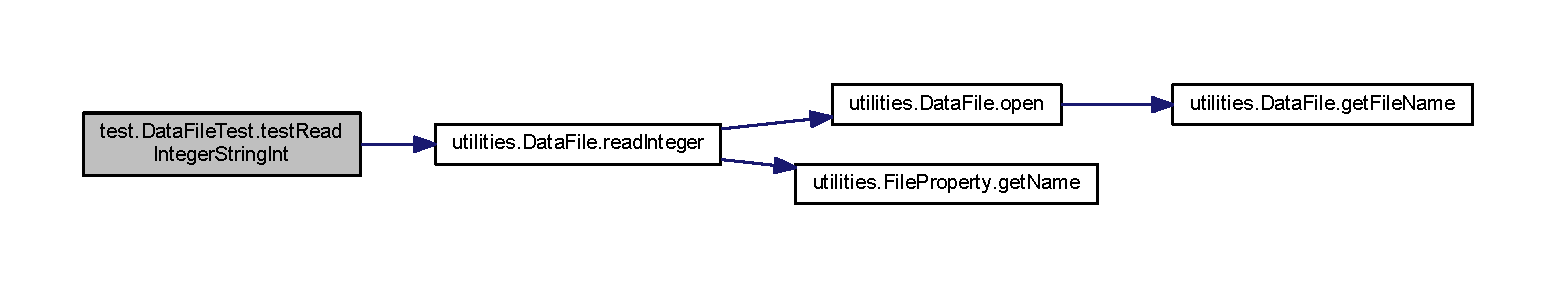
\includegraphics[width=350pt]{classtest_1_1_data_file_test_aa614885277711640980410c5faa5b609_cgraph}
\end{center}
\end{figure}
\mbox{\Hypertarget{classtest_1_1_data_file_test_ad4b0d957eebabf51055d0e7c8be254e7}\label{classtest_1_1_data_file_test_ad4b0d957eebabf51055d0e7c8be254e7}} 
\index{test\+::\+Data\+File\+Test@{test\+::\+Data\+File\+Test}!test\+Read\+List\+String@{test\+Read\+List\+String}}
\index{test\+Read\+List\+String@{test\+Read\+List\+String}!test\+::\+Data\+File\+Test@{test\+::\+Data\+File\+Test}}
\subsubsection{\texorpdfstring{test\+Read\+List\+String()}{testReadListString()}}
{\footnotesize\ttfamily void test.\+Data\+File\+Test.\+test\+Read\+List\+String (\begin{DoxyParamCaption}{ }\end{DoxyParamCaption})}

Here is the call graph for this function\+:\nopagebreak
\begin{figure}[H]
\begin{center}
\leavevmode
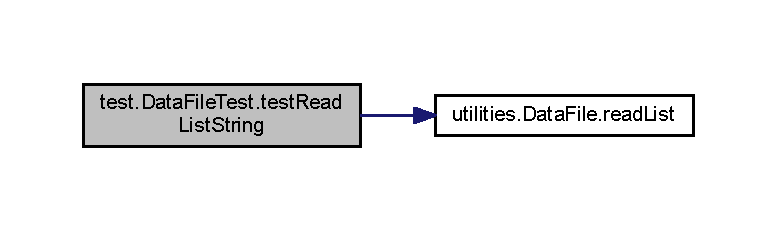
\includegraphics[width=350pt]{classtest_1_1_data_file_test_ad4b0d957eebabf51055d0e7c8be254e7_cgraph}
\end{center}
\end{figure}
\mbox{\Hypertarget{classtest_1_1_data_file_test_ab61a29d98e2d1b08099008e0a5c53b63}\label{classtest_1_1_data_file_test_ab61a29d98e2d1b08099008e0a5c53b63}} 
\index{test\+::\+Data\+File\+Test@{test\+::\+Data\+File\+Test}!test\+Read\+List\+String\+Int@{test\+Read\+List\+String\+Int}}
\index{test\+Read\+List\+String\+Int@{test\+Read\+List\+String\+Int}!test\+::\+Data\+File\+Test@{test\+::\+Data\+File\+Test}}
\subsubsection{\texorpdfstring{test\+Read\+List\+String\+Int()}{testReadListStringInt()}}
{\footnotesize\ttfamily void test.\+Data\+File\+Test.\+test\+Read\+List\+String\+Int (\begin{DoxyParamCaption}{ }\end{DoxyParamCaption})}

Here is the call graph for this function\+:\nopagebreak
\begin{figure}[H]
\begin{center}
\leavevmode
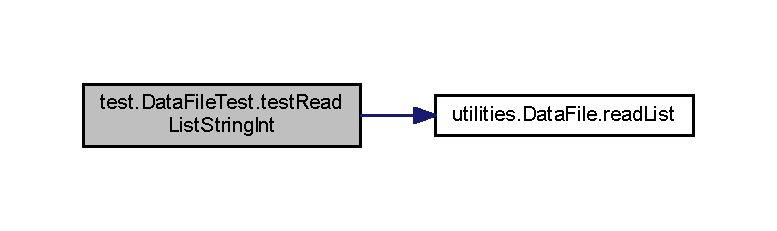
\includegraphics[width=350pt]{classtest_1_1_data_file_test_ab61a29d98e2d1b08099008e0a5c53b63_cgraph}
\end{center}
\end{figure}
\mbox{\Hypertarget{classtest_1_1_data_file_test_ad4298b1da8ab563a46e4adfdc3d15720}\label{classtest_1_1_data_file_test_ad4298b1da8ab563a46e4adfdc3d15720}} 
\index{test\+::\+Data\+File\+Test@{test\+::\+Data\+File\+Test}!test\+Read\+Literal\+Operand\+String\+Int@{test\+Read\+Literal\+Operand\+String\+Int}}
\index{test\+Read\+Literal\+Operand\+String\+Int@{test\+Read\+Literal\+Operand\+String\+Int}!test\+::\+Data\+File\+Test@{test\+::\+Data\+File\+Test}}
\subsubsection{\texorpdfstring{test\+Read\+Literal\+Operand\+String\+Int()}{testReadLiteralOperandStringInt()}}
{\footnotesize\ttfamily void test.\+Data\+File\+Test.\+test\+Read\+Literal\+Operand\+String\+Int (\begin{DoxyParamCaption}{ }\end{DoxyParamCaption})}

Here is the call graph for this function\+:\nopagebreak
\begin{figure}[H]
\begin{center}
\leavevmode
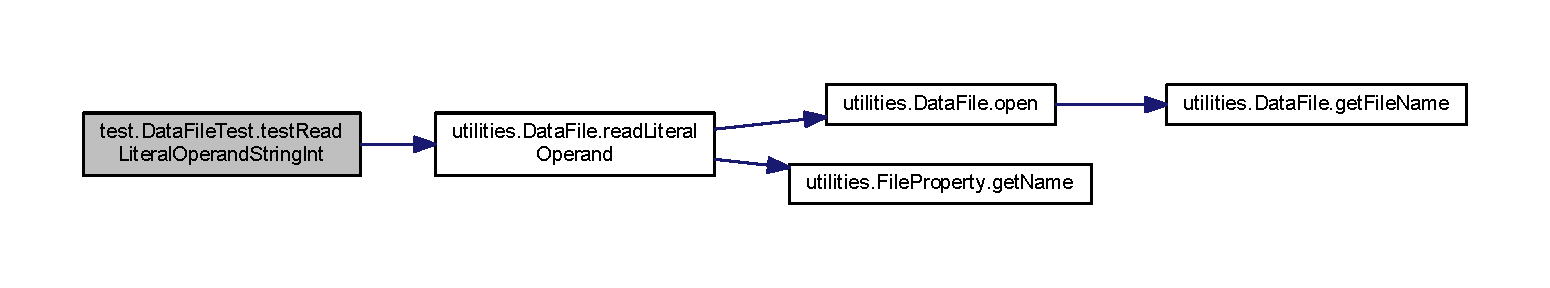
\includegraphics[width=350pt]{classtest_1_1_data_file_test_ad4298b1da8ab563a46e4adfdc3d15720_cgraph}
\end{center}
\end{figure}


The documentation for this class was generated from the following file\+:\begin{DoxyCompactItemize}
\item 
D\+:/workspace/\+Train\+Vagas/src/test/\hyperlink{_data_file_test_8java}{Data\+File\+Test.\+java}\end{DoxyCompactItemize}

\hypertarget{classfrontend_1_1_display}{}\section{frontend.\+Display Class Reference}
\label{classfrontend_1_1_display}\index{frontend.\+Display@{frontend.\+Display}}
\subsection*{Static Public Member Functions}
\begin{DoxyCompactItemize}
\item 
static void \hyperlink{classfrontend_1_1_display_a80dcb9108b718e006f2f97f287619236}{show\+All\+Results} ()
\end{DoxyCompactItemize}
\subsection*{Static Package Attributes}
\begin{DoxyCompactItemize}
\item 
static int \hyperlink{classfrontend_1_1_display_a797d702fc749e192653dc7ff22f2b7d3}{index\+\_\+line} = 1
\item 
static final String \hyperlink{classfrontend_1_1_display_a3202ef0fbf05daddfc35487906120bf4}{F\+O\+R\+M\+A\+T\+\_\+\+D\+O\+U\+B\+LE} = \char`\"{}\%.\+0f\char`\"{}
\item 
static final String \hyperlink{classfrontend_1_1_display_a1db97f649b144d230b033c755d295919}{F\+O\+R\+M\+A\+T\+\_\+\+D\+E\+C\+I\+M\+AL} = \char`\"{}\%d\char`\"{}
\item 
static final String \hyperlink{classfrontend_1_1_display_ab921c44addef8a93aa1315d71a7cdeec}{F\+O\+R\+M\+A\+T\+\_\+\+R\+O\+U\+TE} = \char`\"{}\mbox{[}\%s\mbox{]} \char`\"{}
\item 
static final String \hyperlink{classfrontend_1_1_display_a9a97059c1e7fc38f14b04f12caf7cca7}{F\+O\+R\+M\+A\+T\+\_\+\+S\+T\+R\+I\+NG} = \char`\"{}\%-\/20s\char`\"{}
\item 
static final String \hyperlink{classfrontend_1_1_display_a3a734a034b56b660fdba49e5c5283978}{F\+O\+R\+M\+A\+T\+\_\+\+C\+O\+L1} = \char`\"{}\%-\/7s\char`\"{}
\item 
static final String \hyperlink{classfrontend_1_1_display_a28290e54b617dbdaf5bfdb6c17a78e23}{S\+E\+P\+A\+R\+A\+T\+OR} = \char`\"{} $\vert$ \char`\"{}
\item 
static final String \hyperlink{classfrontend_1_1_display_a7724180a6e1ef99585bcb779b8800480}{N\+E\+W\+\_\+\+L\+I\+NE} = \char`\"{}\textbackslash{}n\char`\"{}
\end{DoxyCompactItemize}
\subsection*{Static Private Member Functions}
\begin{DoxyCompactItemize}
\item 
static void \hyperlink{classfrontend_1_1_display_a6704fd4ef43902afcf1bd072acc5dc71}{print\+Head} ()
\item 
static void \hyperlink{classfrontend_1_1_display_ab2cef6740e59b37091b0215cf82a12f8}{print\+Result\+Shortest} (Map$<$ String, \hyperlink{classdomain_1_1_route}{Route}\mbox{[}$\,$\mbox{]}$>$ shortest)
\item 
static void \hyperlink{classfrontend_1_1_display_a891f43b99b7c9ff439b8eb0544774f48}{print\+Result\+Calculate\+Distance} (\hyperlink{classdomain_1_1_route}{Route}\mbox{[}$\,$\mbox{]} routes)
\item 
static void \hyperlink{classfrontend_1_1_display_a7480b033057115a5237b26915b52bbf4}{print\+Result\+Filter} (\hyperlink{classdomain_1_1_route}{Route}\mbox{[}$\,$\mbox{]} routes)
\item 
static void \hyperlink{classfrontend_1_1_display_a193f8320f4b5d03906180bed773b8f52}{print\+Line} (String line)
\end{DoxyCompactItemize}


\subsection{Member Function Documentation}
\mbox{\Hypertarget{classfrontend_1_1_display_a6704fd4ef43902afcf1bd072acc5dc71}\label{classfrontend_1_1_display_a6704fd4ef43902afcf1bd072acc5dc71}} 
\index{frontend\+::\+Display@{frontend\+::\+Display}!print\+Head@{print\+Head}}
\index{print\+Head@{print\+Head}!frontend\+::\+Display@{frontend\+::\+Display}}
\subsubsection{\texorpdfstring{print\+Head()}{printHead()}}
{\footnotesize\ttfamily static void frontend.\+Display.\+print\+Head (\begin{DoxyParamCaption}{ }\end{DoxyParamCaption})\hspace{0.3cm}{\ttfamily [static]}, {\ttfamily [private]}}

Imprime cabecalho Here is the caller graph for this function\+:\nopagebreak
\begin{figure}[H]
\begin{center}
\leavevmode
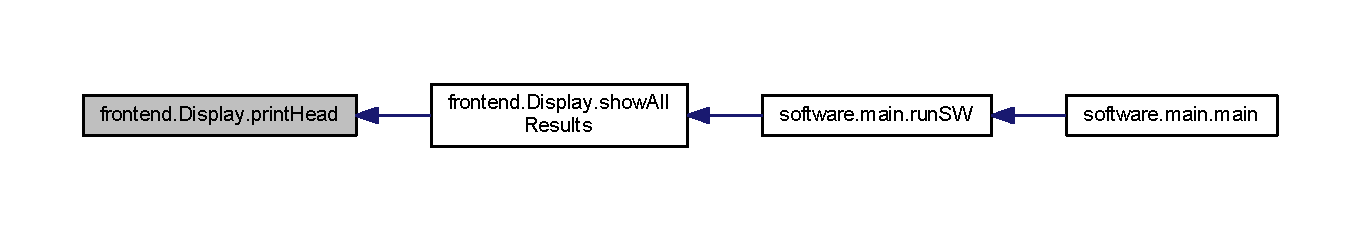
\includegraphics[width=350pt]{classfrontend_1_1_display_a6704fd4ef43902afcf1bd072acc5dc71_icgraph}
\end{center}
\end{figure}
\mbox{\Hypertarget{classfrontend_1_1_display_a193f8320f4b5d03906180bed773b8f52}\label{classfrontend_1_1_display_a193f8320f4b5d03906180bed773b8f52}} 
\index{frontend\+::\+Display@{frontend\+::\+Display}!print\+Line@{print\+Line}}
\index{print\+Line@{print\+Line}!frontend\+::\+Display@{frontend\+::\+Display}}
\subsubsection{\texorpdfstring{print\+Line()}{printLine()}}
{\footnotesize\ttfamily static void frontend.\+Display.\+print\+Line (\begin{DoxyParamCaption}\item[{String}]{line }\end{DoxyParamCaption})\hspace{0.3cm}{\ttfamily [static]}, {\ttfamily [private]}}

Imprime a linha na tela adicionando o numero da linha


\begin{DoxyParams}{Parameters}
{\em line} & Formatada e tabulada \\
\hline
\end{DoxyParams}
Here is the caller graph for this function\+:\nopagebreak
\begin{figure}[H]
\begin{center}
\leavevmode
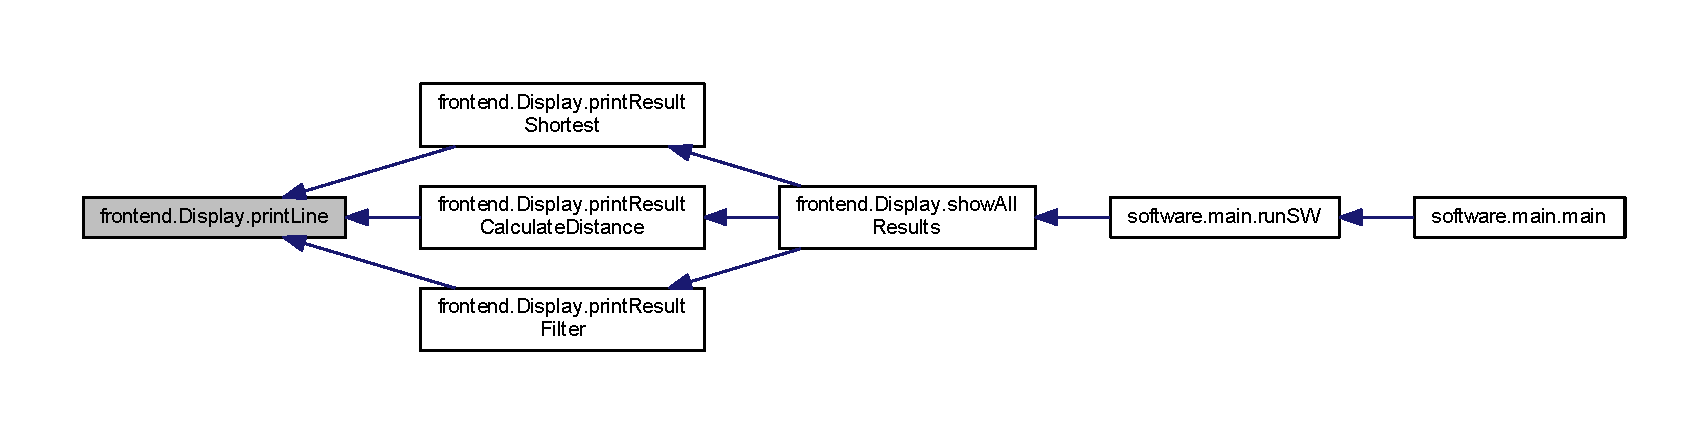
\includegraphics[width=350pt]{classfrontend_1_1_display_a193f8320f4b5d03906180bed773b8f52_icgraph}
\end{center}
\end{figure}
\mbox{\Hypertarget{classfrontend_1_1_display_a891f43b99b7c9ff439b8eb0544774f48}\label{classfrontend_1_1_display_a891f43b99b7c9ff439b8eb0544774f48}} 
\index{frontend\+::\+Display@{frontend\+::\+Display}!print\+Result\+Calculate\+Distance@{print\+Result\+Calculate\+Distance}}
\index{print\+Result\+Calculate\+Distance@{print\+Result\+Calculate\+Distance}!frontend\+::\+Display@{frontend\+::\+Display}}
\subsubsection{\texorpdfstring{print\+Result\+Calculate\+Distance()}{printResultCalculateDistance()}}
{\footnotesize\ttfamily static void frontend.\+Display.\+print\+Result\+Calculate\+Distance (\begin{DoxyParamCaption}\item[{\hyperlink{classdomain_1_1_route}{Route} \mbox{[}$\,$\mbox{]}}]{routes }\end{DoxyParamCaption})\hspace{0.3cm}{\ttfamily [static]}, {\ttfamily [private]}}

Imprime resultado dos calculos de distancias das rotas


\begin{DoxyParams}{Parameters}
{\em routes} & Lista das rotas e seus respectivo valores de distancia \\
\hline
\end{DoxyParams}
Here is the call graph for this function\+:\nopagebreak
\begin{figure}[H]
\begin{center}
\leavevmode
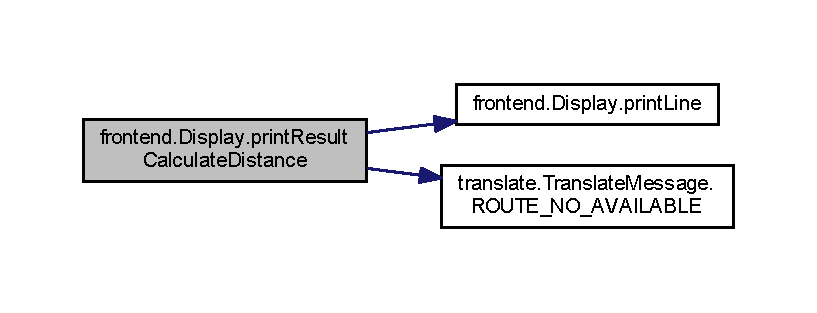
\includegraphics[width=350pt]{classfrontend_1_1_display_a891f43b99b7c9ff439b8eb0544774f48_cgraph}
\end{center}
\end{figure}
Here is the caller graph for this function\+:\nopagebreak
\begin{figure}[H]
\begin{center}
\leavevmode
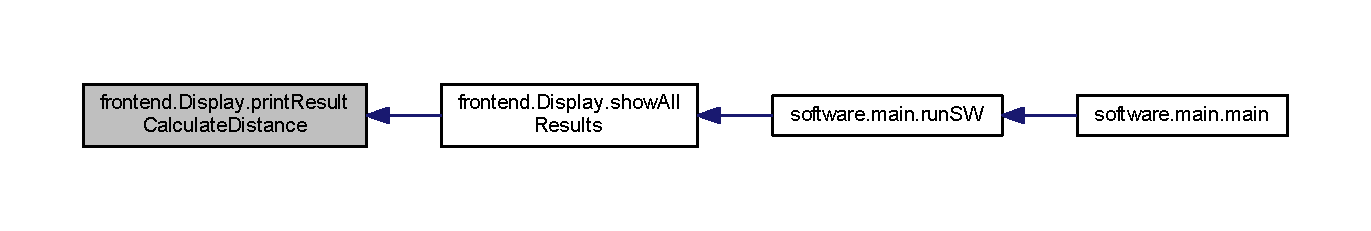
\includegraphics[width=350pt]{classfrontend_1_1_display_a891f43b99b7c9ff439b8eb0544774f48_icgraph}
\end{center}
\end{figure}
\mbox{\Hypertarget{classfrontend_1_1_display_a7480b033057115a5237b26915b52bbf4}\label{classfrontend_1_1_display_a7480b033057115a5237b26915b52bbf4}} 
\index{frontend\+::\+Display@{frontend\+::\+Display}!print\+Result\+Filter@{print\+Result\+Filter}}
\index{print\+Result\+Filter@{print\+Result\+Filter}!frontend\+::\+Display@{frontend\+::\+Display}}
\subsubsection{\texorpdfstring{print\+Result\+Filter()}{printResultFilter()}}
{\footnotesize\ttfamily static void frontend.\+Display.\+print\+Result\+Filter (\begin{DoxyParamCaption}\item[{\hyperlink{classdomain_1_1_route}{Route} \mbox{[}$\,$\mbox{]}}]{routes }\end{DoxyParamCaption})\hspace{0.3cm}{\ttfamily [static]}, {\ttfamily [private]}}

Imprime resultados dos filtros


\begin{DoxyParams}{Parameters}
{\em routes} & \\
\hline
\end{DoxyParams}
Here is the call graph for this function\+:\nopagebreak
\begin{figure}[H]
\begin{center}
\leavevmode
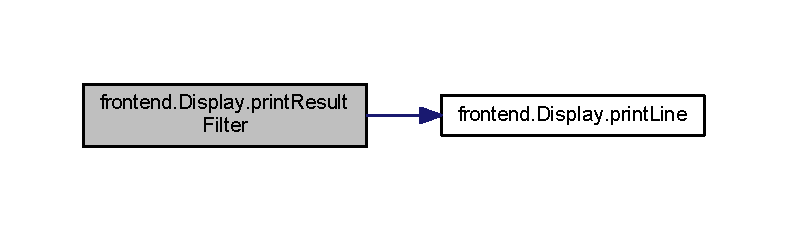
\includegraphics[width=350pt]{classfrontend_1_1_display_a7480b033057115a5237b26915b52bbf4_cgraph}
\end{center}
\end{figure}
Here is the caller graph for this function\+:\nopagebreak
\begin{figure}[H]
\begin{center}
\leavevmode
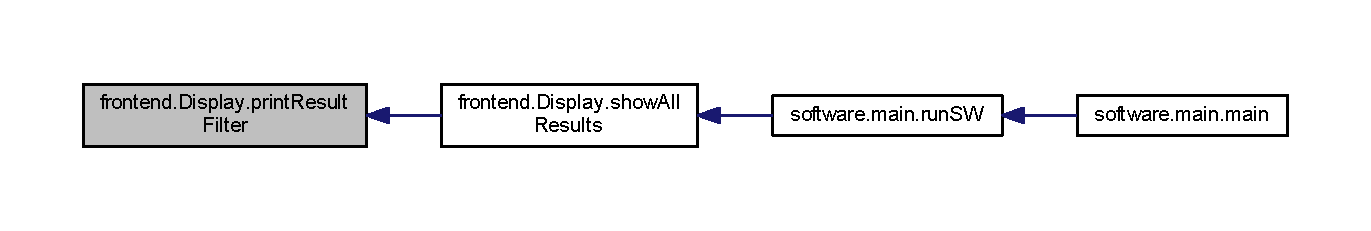
\includegraphics[width=350pt]{classfrontend_1_1_display_a7480b033057115a5237b26915b52bbf4_icgraph}
\end{center}
\end{figure}
\mbox{\Hypertarget{classfrontend_1_1_display_ab2cef6740e59b37091b0215cf82a12f8}\label{classfrontend_1_1_display_ab2cef6740e59b37091b0215cf82a12f8}} 
\index{frontend\+::\+Display@{frontend\+::\+Display}!print\+Result\+Shortest@{print\+Result\+Shortest}}
\index{print\+Result\+Shortest@{print\+Result\+Shortest}!frontend\+::\+Display@{frontend\+::\+Display}}
\subsubsection{\texorpdfstring{print\+Result\+Shortest()}{printResultShortest()}}
{\footnotesize\ttfamily static void frontend.\+Display.\+print\+Result\+Shortest (\begin{DoxyParamCaption}\item[{Map$<$ String, \hyperlink{classdomain_1_1_route}{Route}\mbox{[}$\,$\mbox{]}$>$}]{shortest }\end{DoxyParamCaption})\hspace{0.3cm}{\ttfamily [static]}, {\ttfamily [private]}}

Imprime resulatado relacionado da consulta de menores rotas


\begin{DoxyParams}{Parameters}
{\em shortesd} & Lista das menores rotas \\
\hline
\end{DoxyParams}
Here is the call graph for this function\+:\nopagebreak
\begin{figure}[H]
\begin{center}
\leavevmode
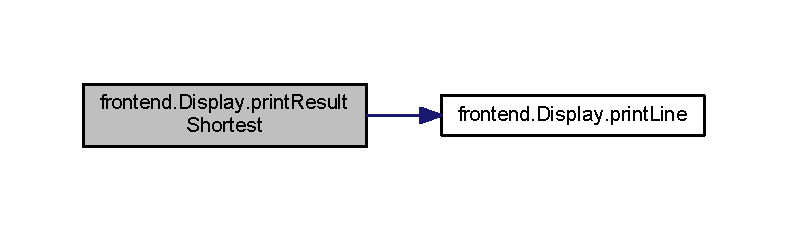
\includegraphics[width=350pt]{classfrontend_1_1_display_ab2cef6740e59b37091b0215cf82a12f8_cgraph}
\end{center}
\end{figure}
Here is the caller graph for this function\+:\nopagebreak
\begin{figure}[H]
\begin{center}
\leavevmode
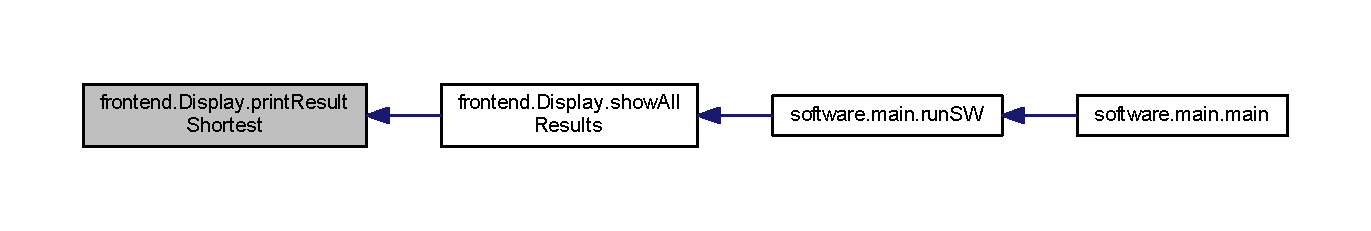
\includegraphics[width=350pt]{classfrontend_1_1_display_ab2cef6740e59b37091b0215cf82a12f8_icgraph}
\end{center}
\end{figure}
\mbox{\Hypertarget{classfrontend_1_1_display_a80dcb9108b718e006f2f97f287619236}\label{classfrontend_1_1_display_a80dcb9108b718e006f2f97f287619236}} 
\index{frontend\+::\+Display@{frontend\+::\+Display}!show\+All\+Results@{show\+All\+Results}}
\index{show\+All\+Results@{show\+All\+Results}!frontend\+::\+Display@{frontend\+::\+Display}}
\subsubsection{\texorpdfstring{show\+All\+Results()}{showAllResults()}}
{\footnotesize\ttfamily static void frontend.\+Display.\+show\+All\+Results (\begin{DoxyParamCaption}{ }\end{DoxyParamCaption})\hspace{0.3cm}{\ttfamily [static]}}

Mostra todos os resultados. Here is the call graph for this function\+:\nopagebreak
\begin{figure}[H]
\begin{center}
\leavevmode
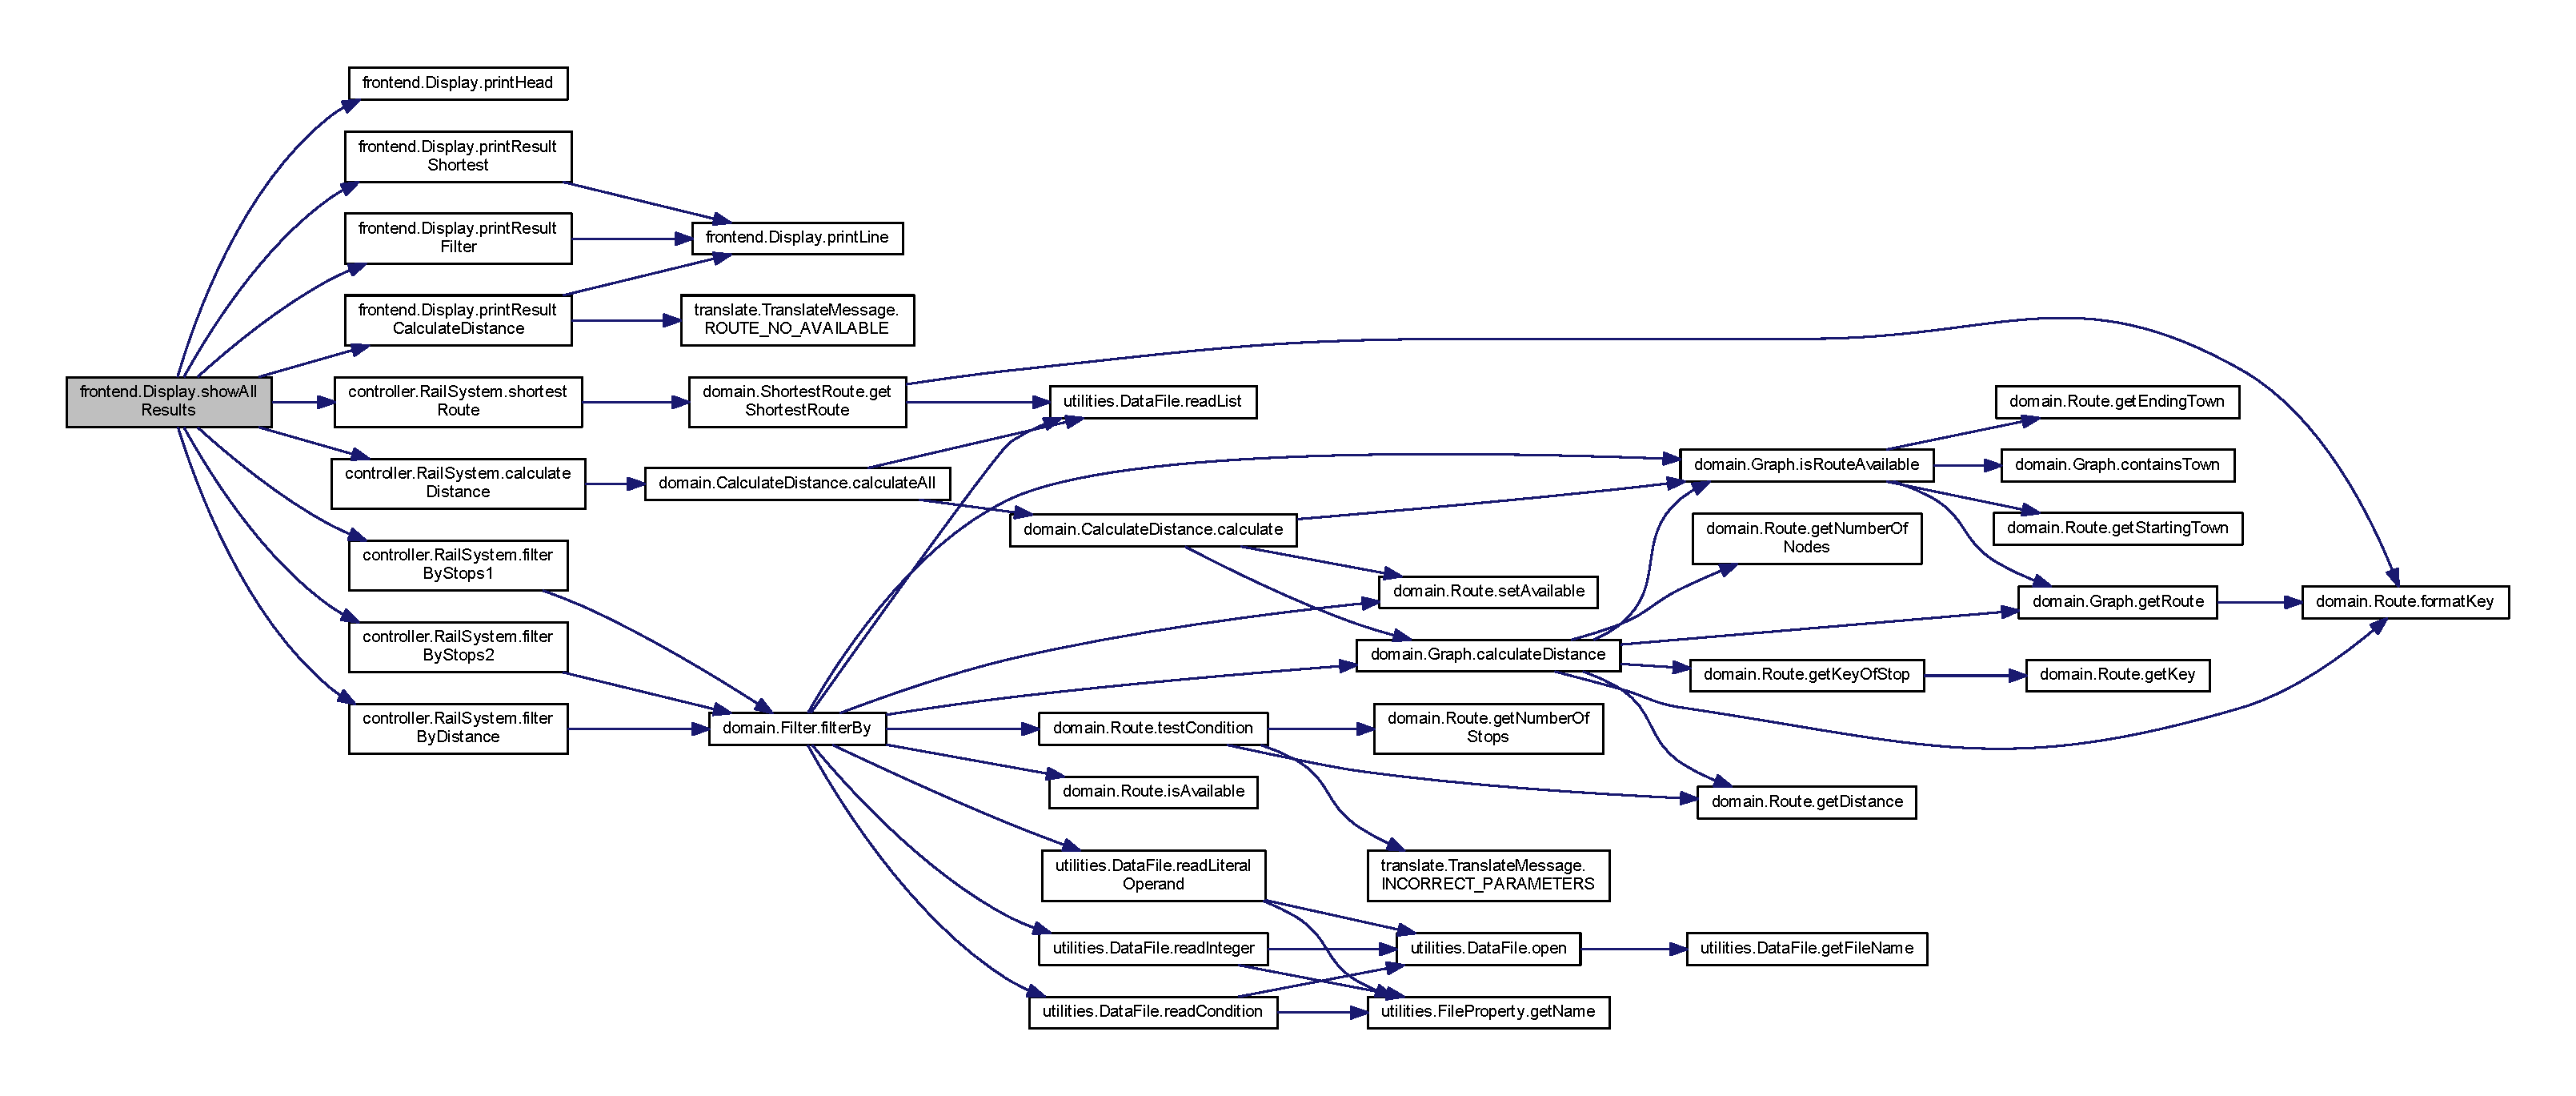
\includegraphics[width=350pt]{classfrontend_1_1_display_a80dcb9108b718e006f2f97f287619236_cgraph}
\end{center}
\end{figure}
Here is the caller graph for this function\+:\nopagebreak
\begin{figure}[H]
\begin{center}
\leavevmode
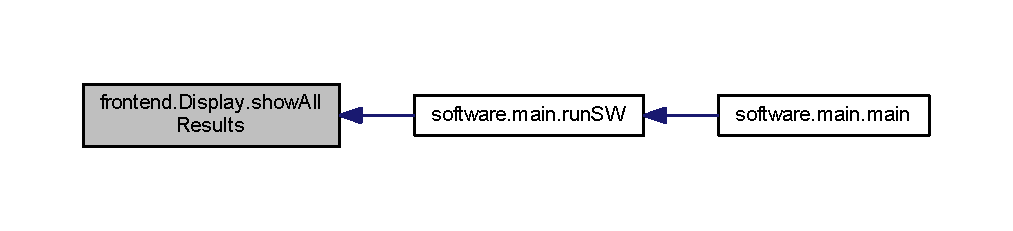
\includegraphics[width=350pt]{classfrontend_1_1_display_a80dcb9108b718e006f2f97f287619236_icgraph}
\end{center}
\end{figure}


\subsection{Member Data Documentation}
\mbox{\Hypertarget{classfrontend_1_1_display_a3a734a034b56b660fdba49e5c5283978}\label{classfrontend_1_1_display_a3a734a034b56b660fdba49e5c5283978}} 
\index{frontend\+::\+Display@{frontend\+::\+Display}!F\+O\+R\+M\+A\+T\+\_\+\+C\+O\+L1@{F\+O\+R\+M\+A\+T\+\_\+\+C\+O\+L1}}
\index{F\+O\+R\+M\+A\+T\+\_\+\+C\+O\+L1@{F\+O\+R\+M\+A\+T\+\_\+\+C\+O\+L1}!frontend\+::\+Display@{frontend\+::\+Display}}
\subsubsection{\texorpdfstring{F\+O\+R\+M\+A\+T\+\_\+\+C\+O\+L1}{FORMAT\_COL1}}
{\footnotesize\ttfamily final String frontend.\+Display.\+F\+O\+R\+M\+A\+T\+\_\+\+C\+O\+L1 = \char`\"{}\%-\/7s\char`\"{}\hspace{0.3cm}{\ttfamily [static]}, {\ttfamily [package]}}

\mbox{\Hypertarget{classfrontend_1_1_display_a1db97f649b144d230b033c755d295919}\label{classfrontend_1_1_display_a1db97f649b144d230b033c755d295919}} 
\index{frontend\+::\+Display@{frontend\+::\+Display}!F\+O\+R\+M\+A\+T\+\_\+\+D\+E\+C\+I\+M\+AL@{F\+O\+R\+M\+A\+T\+\_\+\+D\+E\+C\+I\+M\+AL}}
\index{F\+O\+R\+M\+A\+T\+\_\+\+D\+E\+C\+I\+M\+AL@{F\+O\+R\+M\+A\+T\+\_\+\+D\+E\+C\+I\+M\+AL}!frontend\+::\+Display@{frontend\+::\+Display}}
\subsubsection{\texorpdfstring{F\+O\+R\+M\+A\+T\+\_\+\+D\+E\+C\+I\+M\+AL}{FORMAT\_DECIMAL}}
{\footnotesize\ttfamily final String frontend.\+Display.\+F\+O\+R\+M\+A\+T\+\_\+\+D\+E\+C\+I\+M\+AL = \char`\"{}\%d\char`\"{}\hspace{0.3cm}{\ttfamily [static]}, {\ttfamily [package]}}

\mbox{\Hypertarget{classfrontend_1_1_display_a3202ef0fbf05daddfc35487906120bf4}\label{classfrontend_1_1_display_a3202ef0fbf05daddfc35487906120bf4}} 
\index{frontend\+::\+Display@{frontend\+::\+Display}!F\+O\+R\+M\+A\+T\+\_\+\+D\+O\+U\+B\+LE@{F\+O\+R\+M\+A\+T\+\_\+\+D\+O\+U\+B\+LE}}
\index{F\+O\+R\+M\+A\+T\+\_\+\+D\+O\+U\+B\+LE@{F\+O\+R\+M\+A\+T\+\_\+\+D\+O\+U\+B\+LE}!frontend\+::\+Display@{frontend\+::\+Display}}
\subsubsection{\texorpdfstring{F\+O\+R\+M\+A\+T\+\_\+\+D\+O\+U\+B\+LE}{FORMAT\_DOUBLE}}
{\footnotesize\ttfamily final String frontend.\+Display.\+F\+O\+R\+M\+A\+T\+\_\+\+D\+O\+U\+B\+LE = \char`\"{}\%.\+0f\char`\"{}\hspace{0.3cm}{\ttfamily [static]}, {\ttfamily [package]}}

\mbox{\Hypertarget{classfrontend_1_1_display_ab921c44addef8a93aa1315d71a7cdeec}\label{classfrontend_1_1_display_ab921c44addef8a93aa1315d71a7cdeec}} 
\index{frontend\+::\+Display@{frontend\+::\+Display}!F\+O\+R\+M\+A\+T\+\_\+\+R\+O\+U\+TE@{F\+O\+R\+M\+A\+T\+\_\+\+R\+O\+U\+TE}}
\index{F\+O\+R\+M\+A\+T\+\_\+\+R\+O\+U\+TE@{F\+O\+R\+M\+A\+T\+\_\+\+R\+O\+U\+TE}!frontend\+::\+Display@{frontend\+::\+Display}}
\subsubsection{\texorpdfstring{F\+O\+R\+M\+A\+T\+\_\+\+R\+O\+U\+TE}{FORMAT\_ROUTE}}
{\footnotesize\ttfamily final String frontend.\+Display.\+F\+O\+R\+M\+A\+T\+\_\+\+R\+O\+U\+TE = \char`\"{}\mbox{[}\%s\mbox{]} \char`\"{}\hspace{0.3cm}{\ttfamily [static]}, {\ttfamily [package]}}

\mbox{\Hypertarget{classfrontend_1_1_display_a9a97059c1e7fc38f14b04f12caf7cca7}\label{classfrontend_1_1_display_a9a97059c1e7fc38f14b04f12caf7cca7}} 
\index{frontend\+::\+Display@{frontend\+::\+Display}!F\+O\+R\+M\+A\+T\+\_\+\+S\+T\+R\+I\+NG@{F\+O\+R\+M\+A\+T\+\_\+\+S\+T\+R\+I\+NG}}
\index{F\+O\+R\+M\+A\+T\+\_\+\+S\+T\+R\+I\+NG@{F\+O\+R\+M\+A\+T\+\_\+\+S\+T\+R\+I\+NG}!frontend\+::\+Display@{frontend\+::\+Display}}
\subsubsection{\texorpdfstring{F\+O\+R\+M\+A\+T\+\_\+\+S\+T\+R\+I\+NG}{FORMAT\_STRING}}
{\footnotesize\ttfamily final String frontend.\+Display.\+F\+O\+R\+M\+A\+T\+\_\+\+S\+T\+R\+I\+NG = \char`\"{}\%-\/20s\char`\"{}\hspace{0.3cm}{\ttfamily [static]}, {\ttfamily [package]}}

\mbox{\Hypertarget{classfrontend_1_1_display_a797d702fc749e192653dc7ff22f2b7d3}\label{classfrontend_1_1_display_a797d702fc749e192653dc7ff22f2b7d3}} 
\index{frontend\+::\+Display@{frontend\+::\+Display}!index\+\_\+line@{index\+\_\+line}}
\index{index\+\_\+line@{index\+\_\+line}!frontend\+::\+Display@{frontend\+::\+Display}}
\subsubsection{\texorpdfstring{index\+\_\+line}{index\_line}}
{\footnotesize\ttfamily int frontend.\+Display.\+index\+\_\+line = 1\hspace{0.3cm}{\ttfamily [static]}, {\ttfamily [package]}}

\mbox{\Hypertarget{classfrontend_1_1_display_a7724180a6e1ef99585bcb779b8800480}\label{classfrontend_1_1_display_a7724180a6e1ef99585bcb779b8800480}} 
\index{frontend\+::\+Display@{frontend\+::\+Display}!N\+E\+W\+\_\+\+L\+I\+NE@{N\+E\+W\+\_\+\+L\+I\+NE}}
\index{N\+E\+W\+\_\+\+L\+I\+NE@{N\+E\+W\+\_\+\+L\+I\+NE}!frontend\+::\+Display@{frontend\+::\+Display}}
\subsubsection{\texorpdfstring{N\+E\+W\+\_\+\+L\+I\+NE}{NEW\_LINE}}
{\footnotesize\ttfamily final String frontend.\+Display.\+N\+E\+W\+\_\+\+L\+I\+NE = \char`\"{}\textbackslash{}n\char`\"{}\hspace{0.3cm}{\ttfamily [static]}, {\ttfamily [package]}}

\mbox{\Hypertarget{classfrontend_1_1_display_a28290e54b617dbdaf5bfdb6c17a78e23}\label{classfrontend_1_1_display_a28290e54b617dbdaf5bfdb6c17a78e23}} 
\index{frontend\+::\+Display@{frontend\+::\+Display}!S\+E\+P\+A\+R\+A\+T\+OR@{S\+E\+P\+A\+R\+A\+T\+OR}}
\index{S\+E\+P\+A\+R\+A\+T\+OR@{S\+E\+P\+A\+R\+A\+T\+OR}!frontend\+::\+Display@{frontend\+::\+Display}}
\subsubsection{\texorpdfstring{S\+E\+P\+A\+R\+A\+T\+OR}{SEPARATOR}}
{\footnotesize\ttfamily final String frontend.\+Display.\+S\+E\+P\+A\+R\+A\+T\+OR = \char`\"{} $\vert$ \char`\"{}\hspace{0.3cm}{\ttfamily [static]}, {\ttfamily [package]}}



The documentation for this class was generated from the following file\+:\begin{DoxyCompactItemize}
\item 
D\+:/workspace/\+Train\+Vagas/src/frontend/\hyperlink{_display_8java}{Display.\+java}\end{DoxyCompactItemize}

\hypertarget{enumutilities_1_1_file_property}{}\section{utilities.\+File\+Property Enum Reference}
\label{enumutilities_1_1_file_property}\index{utilities.\+File\+Property@{utilities.\+File\+Property}}
\subsection*{Public Member Functions}
\begin{DoxyCompactItemize}
\item 
\hyperlink{enumutilities_1_1_file_property_ae5d3cd75fb3b377b2e9570490d54f8af}{File\+Property} (String \hyperlink{enumutilities_1_1_file_property_a85714af226bffac084d6264b5bac15d7}{name})
\item 
String \hyperlink{enumutilities_1_1_file_property_ab7c90f768108531dd4468878da2f452d}{get\+Name} ()
\end{DoxyCompactItemize}
\subsection*{Public Attributes}
\begin{DoxyCompactItemize}
\item 
\hyperlink{enumutilities_1_1_file_property_a057ee24e5d0a6a4ca1c9dab2fa0103f1}{G\+R\+A\+P\+H\+\_\+\+R\+O\+U\+T\+ES} =(\char`\"{}graph.\+routes\char`\"{})
\item 
\hyperlink{enumutilities_1_1_file_property_a4d85ea554068d0cfe0de81567126cda1}{D\+I\+S\+T\+A\+N\+C\+E\+\_\+\+R\+O\+U\+T\+ES} =(\char`\"{}distance.\+routes\char`\"{})
\item 
\hyperlink{enumutilities_1_1_file_property_afc45daab73cc6bec29b8c3cb399efa83}{F\+I\+L\+T\+E\+R\+\_\+\+C\+O\+N\+D\+I\+T\+I\+ON} =(\char`\"{}filtertrips\mbox{[}\%d\mbox{]}.condition\char`\"{})
\item 
\hyperlink{enumutilities_1_1_file_property_a86032f5784fe389cae88ea4480bdf0f2}{F\+I\+L\+T\+E\+R\+\_\+\+R\+O\+U\+T\+ES} =(\char`\"{}filtertrips\mbox{[}\%d\mbox{]}.routes\char`\"{})
\item 
\hyperlink{enumutilities_1_1_file_property_ae43a0f6ce3fd6c1cb9ec0e8d42ba2cf0}{S\+H\+O\+R\+T\+E\+S\+T\+\_\+\+R\+O\+U\+T\+ES} =(\char`\"{}shortest\+Router.\+trip\char`\"{})
\end{DoxyCompactItemize}
\subsection*{Private Attributes}
\begin{DoxyCompactItemize}
\item 
String \hyperlink{enumutilities_1_1_file_property_a85714af226bffac084d6264b5bac15d7}{name}
\end{DoxyCompactItemize}


\subsection{Constructor \& Destructor Documentation}
\mbox{\Hypertarget{enumutilities_1_1_file_property_ae5d3cd75fb3b377b2e9570490d54f8af}\label{enumutilities_1_1_file_property_ae5d3cd75fb3b377b2e9570490d54f8af}} 
\index{utilities\+::\+File\+Property@{utilities\+::\+File\+Property}!File\+Property@{File\+Property}}
\index{File\+Property@{File\+Property}!utilities\+::\+File\+Property@{utilities\+::\+File\+Property}}
\subsubsection{\texorpdfstring{File\+Property()}{FileProperty()}}
{\footnotesize\ttfamily utilities.\+File\+Property.\+File\+Property (\begin{DoxyParamCaption}\item[{String}]{name }\end{DoxyParamCaption})}



\subsection{Member Function Documentation}
\mbox{\Hypertarget{enumutilities_1_1_file_property_ab7c90f768108531dd4468878da2f452d}\label{enumutilities_1_1_file_property_ab7c90f768108531dd4468878da2f452d}} 
\index{utilities\+::\+File\+Property@{utilities\+::\+File\+Property}!get\+Name@{get\+Name}}
\index{get\+Name@{get\+Name}!utilities\+::\+File\+Property@{utilities\+::\+File\+Property}}
\subsubsection{\texorpdfstring{get\+Name()}{getName()}}
{\footnotesize\ttfamily String utilities.\+File\+Property.\+get\+Name (\begin{DoxyParamCaption}{ }\end{DoxyParamCaption})}

Here is the caller graph for this function\+:\nopagebreak
\begin{figure}[H]
\begin{center}
\leavevmode
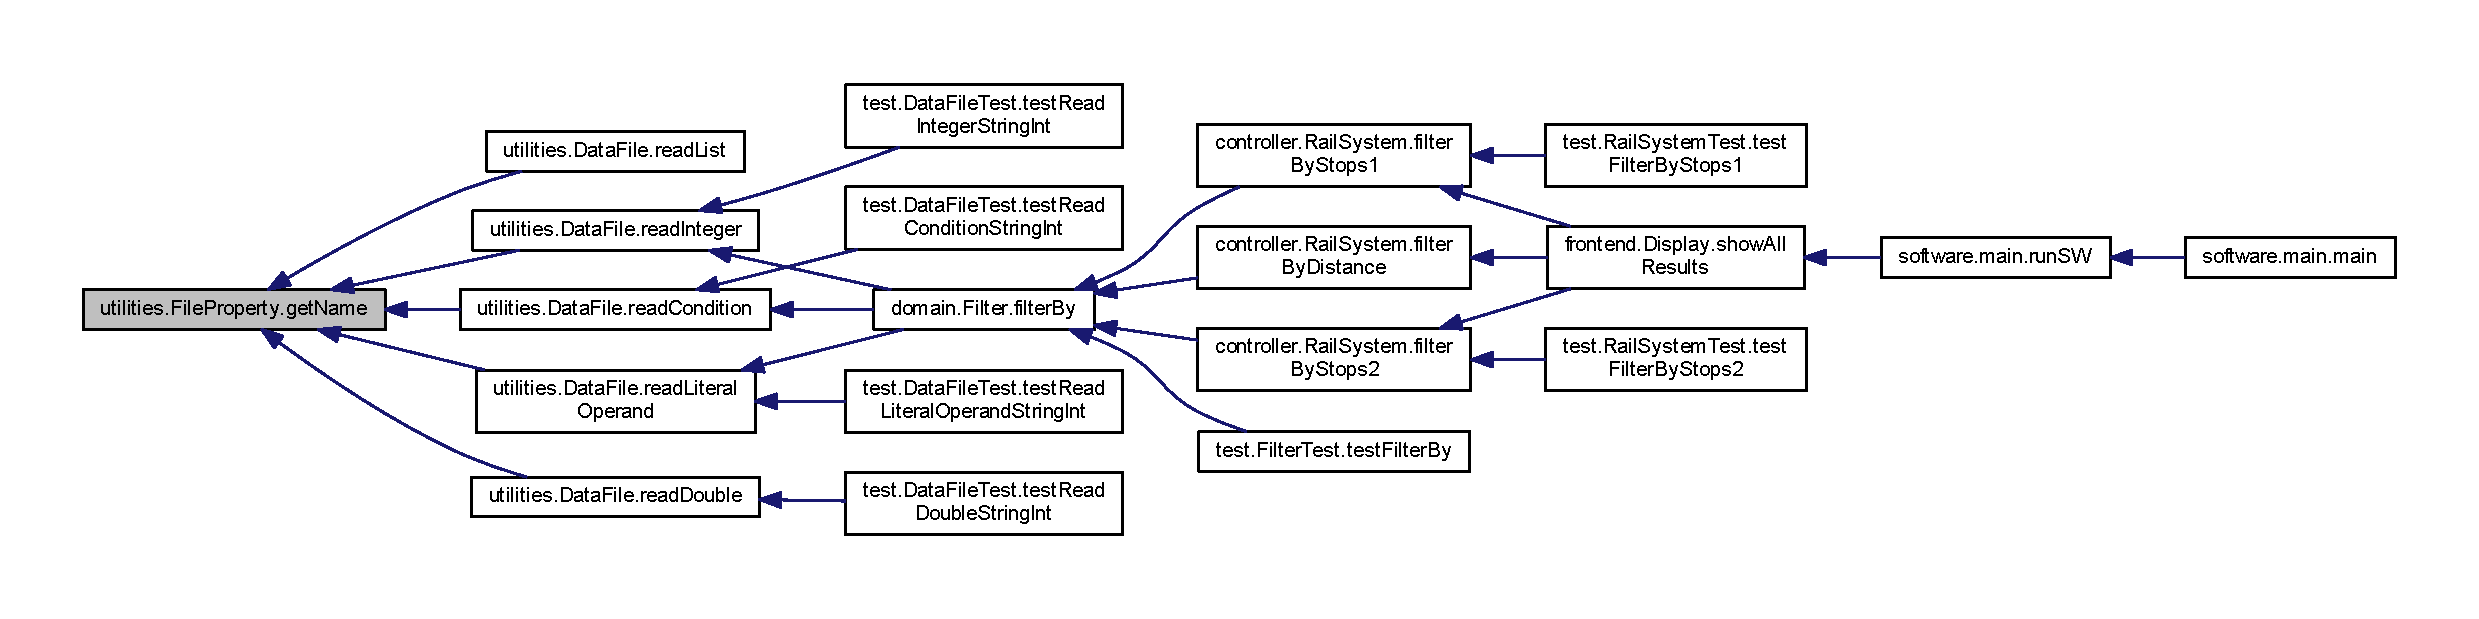
\includegraphics[width=350pt]{enumutilities_1_1_file_property_ab7c90f768108531dd4468878da2f452d_icgraph}
\end{center}
\end{figure}


\subsection{Member Data Documentation}
\mbox{\Hypertarget{enumutilities_1_1_file_property_a4d85ea554068d0cfe0de81567126cda1}\label{enumutilities_1_1_file_property_a4d85ea554068d0cfe0de81567126cda1}} 
\index{utilities\+::\+File\+Property@{utilities\+::\+File\+Property}!D\+I\+S\+T\+A\+N\+C\+E\+\_\+\+R\+O\+U\+T\+ES@{D\+I\+S\+T\+A\+N\+C\+E\+\_\+\+R\+O\+U\+T\+ES}}
\index{D\+I\+S\+T\+A\+N\+C\+E\+\_\+\+R\+O\+U\+T\+ES@{D\+I\+S\+T\+A\+N\+C\+E\+\_\+\+R\+O\+U\+T\+ES}!utilities\+::\+File\+Property@{utilities\+::\+File\+Property}}
\subsubsection{\texorpdfstring{D\+I\+S\+T\+A\+N\+C\+E\+\_\+\+R\+O\+U\+T\+ES}{DISTANCE\_ROUTES}}
{\footnotesize\ttfamily utilities.\+File\+Property.\+D\+I\+S\+T\+A\+N\+C\+E\+\_\+\+R\+O\+U\+T\+ES =(\char`\"{}distance.\+routes\char`\"{})}

Questoes\+: 1) The distance of the route A-\/\+B-\/C. 2) The distance of the route A-\/D. 3) The distance of the route A-\/\+D-\/C. 4) The distance of the route A-\/\+E-\/\+B-\/\+C-\/D. 5) The distance of the route A-\/\+E-\/D.

Mapeamento das rotas para calculo da distancia O hifem e opcional Separador virgula Possibilidade de adiconar novas rotas \mbox{\Hypertarget{enumutilities_1_1_file_property_afc45daab73cc6bec29b8c3cb399efa83}\label{enumutilities_1_1_file_property_afc45daab73cc6bec29b8c3cb399efa83}} 
\index{utilities\+::\+File\+Property@{utilities\+::\+File\+Property}!F\+I\+L\+T\+E\+R\+\_\+\+C\+O\+N\+D\+I\+T\+I\+ON@{F\+I\+L\+T\+E\+R\+\_\+\+C\+O\+N\+D\+I\+T\+I\+ON}}
\index{F\+I\+L\+T\+E\+R\+\_\+\+C\+O\+N\+D\+I\+T\+I\+ON@{F\+I\+L\+T\+E\+R\+\_\+\+C\+O\+N\+D\+I\+T\+I\+ON}!utilities\+::\+File\+Property@{utilities\+::\+File\+Property}}
\subsubsection{\texorpdfstring{F\+I\+L\+T\+E\+R\+\_\+\+C\+O\+N\+D\+I\+T\+I\+ON}{FILTER\_CONDITION}}
{\footnotesize\ttfamily utilities.\+File\+Property.\+F\+I\+L\+T\+E\+R\+\_\+\+C\+O\+N\+D\+I\+T\+I\+ON =(\char`\"{}filtertrips\mbox{[}\%d\mbox{]}.condition\char`\"{})}

Questoes\+: 6) The number of trips starting at C and ending at C with a maximum of 3 stops. In the sample data below, there are two such trips\+: C-\/\+D-\/C (2 stops). and C-\/\+E-\/\+B-\/C (3 stops). 7) The number of trips starting at A and ending at C with exactly 4 stops. In the sample data below, there are three such trips\+: A to C (via B,C,D); A to C (via D,C,D); and A to C (via D,E,B). 10)The number of different routes from C to C with a distance of less than 30. In the sample data, the trips are\+: C\+DC, C\+E\+BC, C\+E\+B\+C\+DC, C\+D\+C\+E\+BC, C\+D\+E\+BC, C\+E\+B\+C\+E\+BC, C\+E\+B\+C\+E\+B\+C\+E\+BC.

Verifica se as rotas indicadas na propriedade filtertrips\mbox{[}X\mbox{]}.routes satifazem a condicao indicada em filtertrips\mbox{[}X\mbox{]}.condition. Condicoes permitidas\+: $<$,$>$,$<$=,$>$=,==,!=. Operandos permitidos S\+T\+O\+PS,D\+I\+S\+T\+A\+N\+CE. O hifem e opcional. Rotas invalidas serao desconsideradas. Importante\+: Separador por virgula. Possibilidade de adiconar novos filtros,diferenciar atraves do index \mbox{[}X\mbox{]}. \mbox{\Hypertarget{enumutilities_1_1_file_property_a86032f5784fe389cae88ea4480bdf0f2}\label{enumutilities_1_1_file_property_a86032f5784fe389cae88ea4480bdf0f2}} 
\index{utilities\+::\+File\+Property@{utilities\+::\+File\+Property}!F\+I\+L\+T\+E\+R\+\_\+\+R\+O\+U\+T\+ES@{F\+I\+L\+T\+E\+R\+\_\+\+R\+O\+U\+T\+ES}}
\index{F\+I\+L\+T\+E\+R\+\_\+\+R\+O\+U\+T\+ES@{F\+I\+L\+T\+E\+R\+\_\+\+R\+O\+U\+T\+ES}!utilities\+::\+File\+Property@{utilities\+::\+File\+Property}}
\subsubsection{\texorpdfstring{F\+I\+L\+T\+E\+R\+\_\+\+R\+O\+U\+T\+ES}{FILTER\_ROUTES}}
{\footnotesize\ttfamily utilities.\+File\+Property.\+F\+I\+L\+T\+E\+R\+\_\+\+R\+O\+U\+T\+ES =(\char`\"{}filtertrips\mbox{[}\%d\mbox{]}.routes\char`\"{})}

\mbox{\Hypertarget{enumutilities_1_1_file_property_a057ee24e5d0a6a4ca1c9dab2fa0103f1}\label{enumutilities_1_1_file_property_a057ee24e5d0a6a4ca1c9dab2fa0103f1}} 
\index{utilities\+::\+File\+Property@{utilities\+::\+File\+Property}!G\+R\+A\+P\+H\+\_\+\+R\+O\+U\+T\+ES@{G\+R\+A\+P\+H\+\_\+\+R\+O\+U\+T\+ES}}
\index{G\+R\+A\+P\+H\+\_\+\+R\+O\+U\+T\+ES@{G\+R\+A\+P\+H\+\_\+\+R\+O\+U\+T\+ES}!utilities\+::\+File\+Property@{utilities\+::\+File\+Property}}
\subsubsection{\texorpdfstring{G\+R\+A\+P\+H\+\_\+\+R\+O\+U\+T\+ES}{GRAPH\_ROUTES}}
{\footnotesize\ttfamily utilities.\+File\+Property.\+G\+R\+A\+P\+H\+\_\+\+R\+O\+U\+T\+ES =(\char`\"{}graph.\+routes\char`\"{})}

Mapa de estacoes

Diagrama esta baseado na descricao do teste. \textquotesingle{}$\ast$\textquotesingle{} Indica rotas de chegada na estacao (D) Indica a distancia \begin{DoxyVerb}  ------------(3)----------------- 
  |                              |
  |                              * 
  | -(7)-[ A ]------(5)-------*[ B ]
  | |      |                     |
  | |     (5)                   (4)
  | |      |                     |
  | *      *                     *
 [ E ]*--[ D ] -----(8)-------*[ C ]
   *          *-----(8)-------   |
   |                             |
   ----------(2)------------------
\end{DoxyVerb}


Mapeamento de todas as rotas disponiveis O SW esta trabalhando dinamicamente, podendo ser adicionadas novas rotas Para numeros decimais usar \textquotesingle{}.\textquotesingle{} Separador por virgula \mbox{\Hypertarget{enumutilities_1_1_file_property_a85714af226bffac084d6264b5bac15d7}\label{enumutilities_1_1_file_property_a85714af226bffac084d6264b5bac15d7}} 
\index{utilities\+::\+File\+Property@{utilities\+::\+File\+Property}!name@{name}}
\index{name@{name}!utilities\+::\+File\+Property@{utilities\+::\+File\+Property}}
\subsubsection{\texorpdfstring{name}{name}}
{\footnotesize\ttfamily String utilities.\+File\+Property.\+name\hspace{0.3cm}{\ttfamily [private]}}

\mbox{\Hypertarget{enumutilities_1_1_file_property_ae43a0f6ce3fd6c1cb9ec0e8d42ba2cf0}\label{enumutilities_1_1_file_property_ae43a0f6ce3fd6c1cb9ec0e8d42ba2cf0}} 
\index{utilities\+::\+File\+Property@{utilities\+::\+File\+Property}!S\+H\+O\+R\+T\+E\+S\+T\+\_\+\+R\+O\+U\+T\+ES@{S\+H\+O\+R\+T\+E\+S\+T\+\_\+\+R\+O\+U\+T\+ES}}
\index{S\+H\+O\+R\+T\+E\+S\+T\+\_\+\+R\+O\+U\+T\+ES@{S\+H\+O\+R\+T\+E\+S\+T\+\_\+\+R\+O\+U\+T\+ES}!utilities\+::\+File\+Property@{utilities\+::\+File\+Property}}
\subsubsection{\texorpdfstring{S\+H\+O\+R\+T\+E\+S\+T\+\_\+\+R\+O\+U\+T\+ES}{SHORTEST\_ROUTES}}
{\footnotesize\ttfamily utilities.\+File\+Property.\+S\+H\+O\+R\+T\+E\+S\+T\+\_\+\+R\+O\+U\+T\+ES =(\char`\"{}shortest\+Router.\+trip\char`\"{})}

Questoes\+: 8) The length of the shortest route (in terms of distance to travel) from A to C. 9) The length of the shortest route (in terms of distance to travel) from B to B.

Encontra as opcoes de rotas menores(distancia) entre o ponto de partida e o de chegada Possibilidade de adiconar quantas viagens(rotas) necessarias. Rotas invalidas serao desconsideradas O hifem e opcional Separador virgula 

The documentation for this enum was generated from the following file\+:\begin{DoxyCompactItemize}
\item 
D\+:/workspace/\+Train\+Vagas/src/utilities/\hyperlink{_file_property_8java}{File\+Property.\+java}\end{DoxyCompactItemize}

\hypertarget{classdomain_1_1_filter}{}\section{domain.\+Filter Class Reference}
\label{classdomain_1_1_filter}\index{domain.\+Filter@{domain.\+Filter}}


Collaboration diagram for domain.\+Filter\+:\nopagebreak
\begin{figure}[H]
\begin{center}
\leavevmode
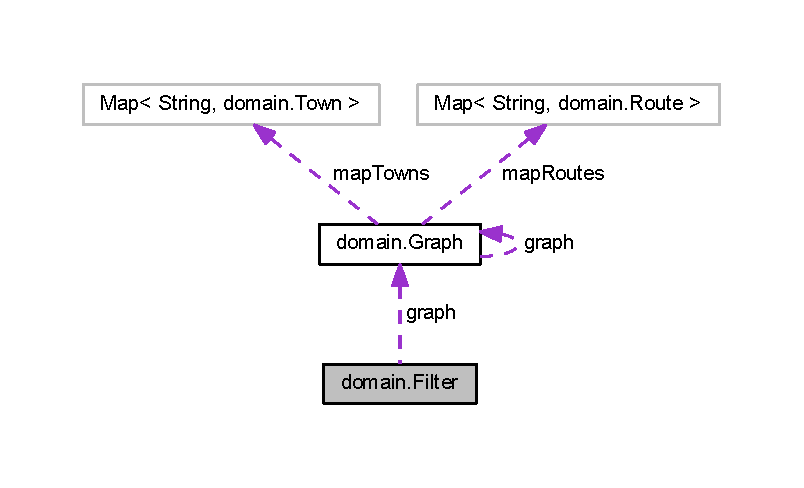
\includegraphics[width=350pt]{classdomain_1_1_filter__coll__graph}
\end{center}
\end{figure}
\subsection*{Public Member Functions}
\begin{DoxyCompactItemize}
\item 
\hyperlink{classdomain_1_1_route}{Route} \mbox{[}$\,$\mbox{]} \hyperlink{classdomain_1_1_filter_a5935a1a7d6f7b13de220ed9b6547b897}{filter\+By} (int index\+\_\+filter)
\end{DoxyCompactItemize}
\subsection*{Package Attributes}
\begin{DoxyCompactItemize}
\item 
\hyperlink{classdomain_1_1_graph}{Graph} \hyperlink{classdomain_1_1_filter_afdd7492ce4c44ba22ad16e3ad819a70c}{graph} = \hyperlink{classdomain_1_1_graph_a57ce4efd344c059a565f4bb104fdee64}{Graph.\+create}()
\end{DoxyCompactItemize}


\subsection{Member Function Documentation}
\mbox{\Hypertarget{classdomain_1_1_filter_a5935a1a7d6f7b13de220ed9b6547b897}\label{classdomain_1_1_filter_a5935a1a7d6f7b13de220ed9b6547b897}} 
\index{domain\+::\+Filter@{domain\+::\+Filter}!filter\+By@{filter\+By}}
\index{filter\+By@{filter\+By}!domain\+::\+Filter@{domain\+::\+Filter}}
\subsubsection{\texorpdfstring{filter\+By()}{filterBy()}}
{\footnotesize\ttfamily \hyperlink{classdomain_1_1_route}{Route} \mbox{[}$\,$\mbox{]} domain.\+Filter.\+filter\+By (\begin{DoxyParamCaption}\item[{int}]{index\+\_\+filter }\end{DoxyParamCaption})}

Verifica se as rotas indicadas no arquivo \textquotesingle{}input.\+txt\textquotesingle{} na propriedade \textquotesingle{}filtertrips\mbox{[}X\mbox{]}.routes\textquotesingle{} satifazem a condicao indicada em \textquotesingle{}filtertrips\mbox{[}X\mbox{]}.condition\textquotesingle{}. Condicoes permitidas\+: \textquotesingle{}$<$\textquotesingle{},\textquotesingle{}$>$\textquotesingle{},\textquotesingle{}$<$=\textquotesingle{},\textquotesingle{}$>$=\textquotesingle{},\textquotesingle{}==\textquotesingle{},\textquotesingle{}!=\textquotesingle{} Operandos permitidos S\+T\+O\+PS,D\+I\+S\+T\+A\+N\+CE Rotas invalidas serao desconsideradas


\begin{DoxyParams}{Parameters}
{\em num\+\_\+test} & indice do filtro \\
\hline
\end{DoxyParams}
\begin{DoxyReturn}{Returns}
Rotas filtradas pela condincao 
\end{DoxyReturn}
Here is the call graph for this function\+:\nopagebreak
\begin{figure}[H]
\begin{center}
\leavevmode
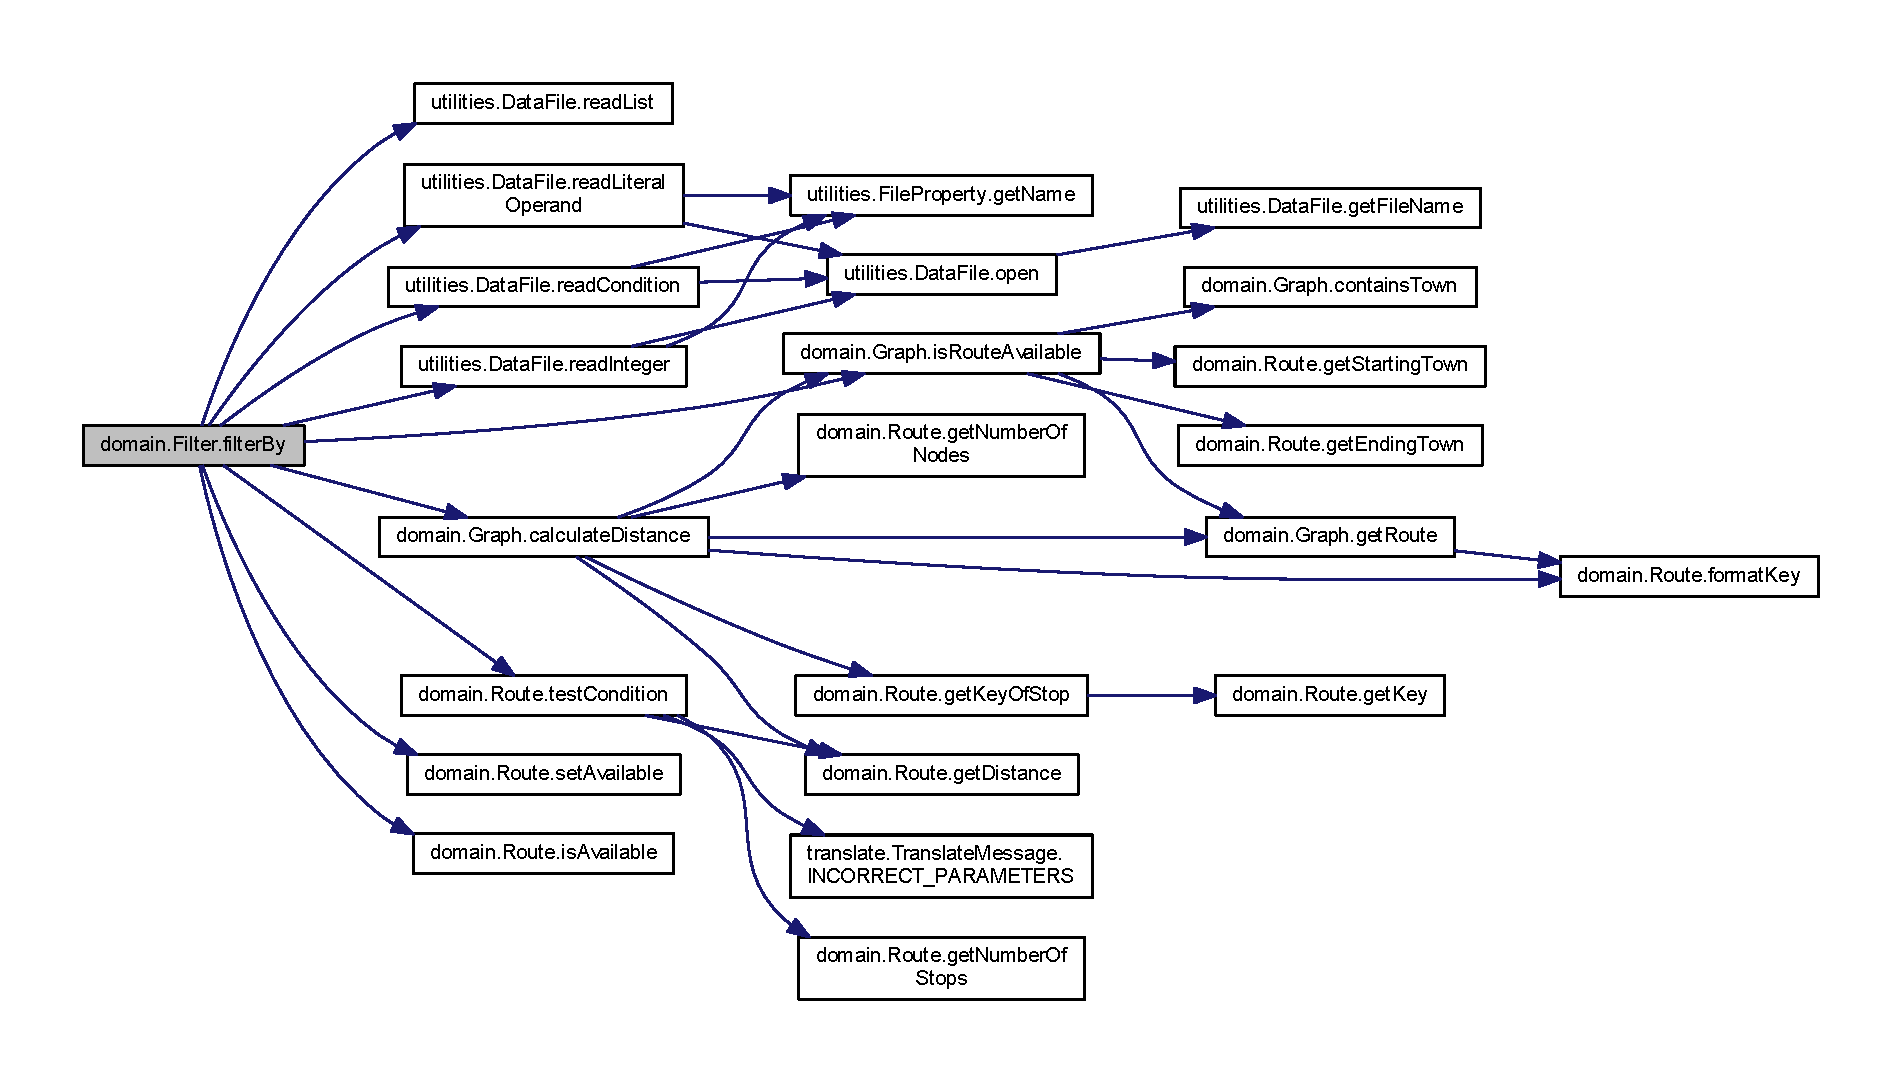
\includegraphics[width=350pt]{classdomain_1_1_filter_a5935a1a7d6f7b13de220ed9b6547b897_cgraph}
\end{center}
\end{figure}
Here is the caller graph for this function\+:\nopagebreak
\begin{figure}[H]
\begin{center}
\leavevmode
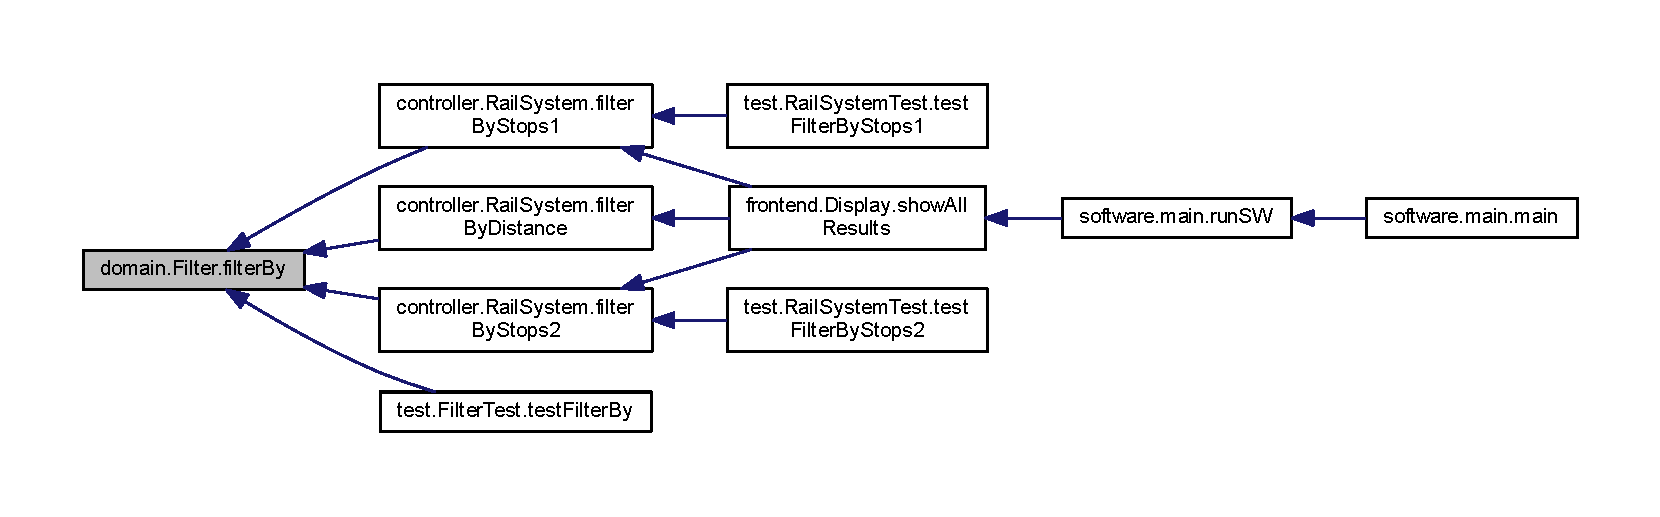
\includegraphics[width=350pt]{classdomain_1_1_filter_a5935a1a7d6f7b13de220ed9b6547b897_icgraph}
\end{center}
\end{figure}


\subsection{Member Data Documentation}
\mbox{\Hypertarget{classdomain_1_1_filter_afdd7492ce4c44ba22ad16e3ad819a70c}\label{classdomain_1_1_filter_afdd7492ce4c44ba22ad16e3ad819a70c}} 
\index{domain\+::\+Filter@{domain\+::\+Filter}!graph@{graph}}
\index{graph@{graph}!domain\+::\+Filter@{domain\+::\+Filter}}
\subsubsection{\texorpdfstring{graph}{graph}}
{\footnotesize\ttfamily \hyperlink{classdomain_1_1_graph}{Graph} domain.\+Filter.\+graph = \hyperlink{classdomain_1_1_graph_a57ce4efd344c059a565f4bb104fdee64}{Graph.\+create}()\hspace{0.3cm}{\ttfamily [package]}}

Rotas disponiveis no sistema 

The documentation for this class was generated from the following file\+:\begin{DoxyCompactItemize}
\item 
D\+:/workspace/\+Train\+Vagas/src/domain/\hyperlink{_filter_8java}{Filter.\+java}\end{DoxyCompactItemize}

\hypertarget{classtest_1_1_filter_test}{}\section{test.\+Filter\+Test Class Reference}
\label{classtest_1_1_filter_test}\index{test.\+Filter\+Test@{test.\+Filter\+Test}}


Collaboration diagram for test.\+Filter\+Test\+:\nopagebreak
\begin{figure}[H]
\begin{center}
\leavevmode
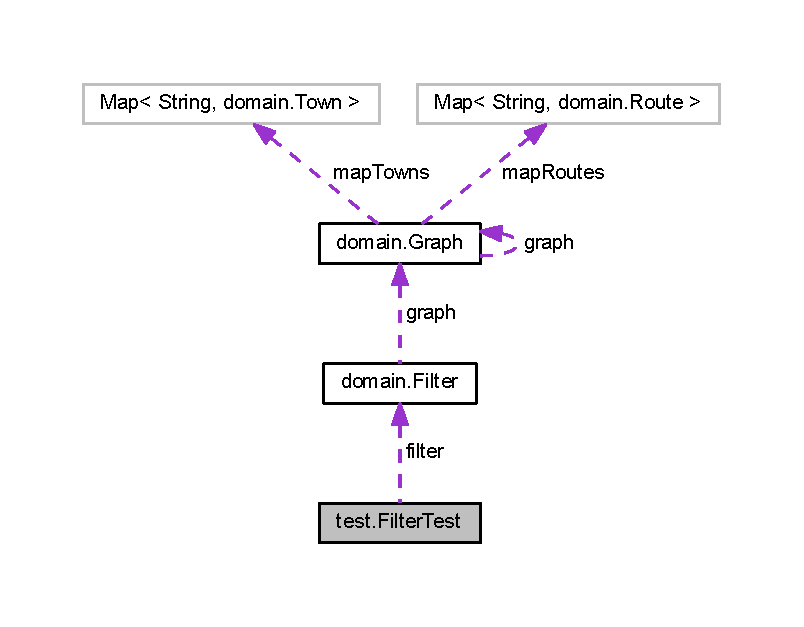
\includegraphics[width=350pt]{classtest_1_1_filter_test__coll__graph}
\end{center}
\end{figure}
\subsection*{Public Member Functions}
\begin{DoxyCompactItemize}
\item 
void \hyperlink{classtest_1_1_filter_test_af76a634a6d91aad982f591ef07c21969}{set\+Up} ()  throws Exception 
\item 
void \hyperlink{classtest_1_1_filter_test_abd2f49938ef9663ecee1953d09bae933}{test\+Filter\+By} ()
\end{DoxyCompactItemize}
\subsection*{Package Attributes}
\begin{DoxyCompactItemize}
\item 
\hyperlink{classdomain_1_1_filter}{Filter} \hyperlink{classtest_1_1_filter_test_ac79abdc8770b75af63e5b8cc190c42c6}{filter}
\end{DoxyCompactItemize}


\subsection{Member Function Documentation}
\mbox{\Hypertarget{classtest_1_1_filter_test_af76a634a6d91aad982f591ef07c21969}\label{classtest_1_1_filter_test_af76a634a6d91aad982f591ef07c21969}} 
\index{test\+::\+Filter\+Test@{test\+::\+Filter\+Test}!set\+Up@{set\+Up}}
\index{set\+Up@{set\+Up}!test\+::\+Filter\+Test@{test\+::\+Filter\+Test}}
\subsubsection{\texorpdfstring{set\+Up()}{setUp()}}
{\footnotesize\ttfamily void test.\+Filter\+Test.\+set\+Up (\begin{DoxyParamCaption}{ }\end{DoxyParamCaption}) throws Exception}

Here is the call graph for this function\+:\nopagebreak
\begin{figure}[H]
\begin{center}
\leavevmode
\includegraphics[width=350pt]{classtest_1_1_filter_test_af76a634a6d91aad982f591ef07c21969_cgraph}
\end{center}
\end{figure}
\mbox{\Hypertarget{classtest_1_1_filter_test_abd2f49938ef9663ecee1953d09bae933}\label{classtest_1_1_filter_test_abd2f49938ef9663ecee1953d09bae933}} 
\index{test\+::\+Filter\+Test@{test\+::\+Filter\+Test}!test\+Filter\+By@{test\+Filter\+By}}
\index{test\+Filter\+By@{test\+Filter\+By}!test\+::\+Filter\+Test@{test\+::\+Filter\+Test}}
\subsubsection{\texorpdfstring{test\+Filter\+By()}{testFilterBy()}}
{\footnotesize\ttfamily void test.\+Filter\+Test.\+test\+Filter\+By (\begin{DoxyParamCaption}{ }\end{DoxyParamCaption})}

Here is the call graph for this function\+:\nopagebreak
\begin{figure}[H]
\begin{center}
\leavevmode
\includegraphics[width=350pt]{classtest_1_1_filter_test_abd2f49938ef9663ecee1953d09bae933_cgraph}
\end{center}
\end{figure}


\subsection{Member Data Documentation}
\mbox{\Hypertarget{classtest_1_1_filter_test_ac79abdc8770b75af63e5b8cc190c42c6}\label{classtest_1_1_filter_test_ac79abdc8770b75af63e5b8cc190c42c6}} 
\index{test\+::\+Filter\+Test@{test\+::\+Filter\+Test}!filter@{filter}}
\index{filter@{filter}!test\+::\+Filter\+Test@{test\+::\+Filter\+Test}}
\subsubsection{\texorpdfstring{filter}{filter}}
{\footnotesize\ttfamily \hyperlink{classdomain_1_1_filter}{Filter} test.\+Filter\+Test.\+filter\hspace{0.3cm}{\ttfamily [package]}}



The documentation for this class was generated from the following file\+:\begin{DoxyCompactItemize}
\item 
D\+:/workspace/\+Train\+Vagas/src/test/\hyperlink{_filter_test_8java}{Filter\+Test.\+java}\end{DoxyCompactItemize}

\hypertarget{classdomain_1_1_graph}{}\section{domain.\+Graph Class Reference}
\label{classdomain_1_1_graph}\index{domain.\+Graph@{domain.\+Graph}}


Collaboration diagram for domain.\+Graph\+:\nopagebreak
\begin{figure}[H]
\begin{center}
\leavevmode
\includegraphics[width=350pt]{classdomain_1_1_graph__coll__graph}
\end{center}
\end{figure}
\subsection*{Public Member Functions}
\begin{DoxyCompactItemize}
\item 
void \hyperlink{classdomain_1_1_graph_ab310780b6719b7b94e8eea0a0603f6c1}{clear} ()
\item 
String \mbox{[}$\,$\mbox{]} \hyperlink{classdomain_1_1_graph_a3789a71ab36974dce8c6c6aac41007f3}{get\+All\+Towns} ()
\item 
String \mbox{[}$\,$\mbox{]} \hyperlink{classdomain_1_1_graph_aa91cc429a4ea1d2c3341baea617e4028}{get\+All\+Routes} ()
\item 
String \mbox{[}$\,$\mbox{]} \hyperlink{classdomain_1_1_graph_a3ceedf597c66f500579a0e302c32062b}{get\+All\+Route\+Possible} (\hyperlink{classdomain_1_1_route}{Route} trip)
\item 
String \mbox{[}$\,$\mbox{]} \hyperlink{classdomain_1_1_graph_adab0f0e6ae7af913998f537aa0fe62f1}{get\+Connections} (String key\+\_\+town)
\item 
void \hyperlink{classdomain_1_1_graph_a2ecd9722f3cbb7d97fda519101d249ed}{add\+Route} (String key\+\_\+route)
\item 
void \hyperlink{classdomain_1_1_graph_a356a31b6dba042cccb2a743caa07bfdf}{add\+Route} (String\mbox{[}$\,$\mbox{]}routes)
\item 
void \hyperlink{classdomain_1_1_graph_a93f040b758a5f920d195f2fbfdccc741}{add\+Town} (String key\+\_\+town)
\item 
\hyperlink{classdomain_1_1_route}{Route} \hyperlink{classdomain_1_1_graph_a3499aec1dfba7e73b34007cb4271e192}{get\+Route} (String key\+\_\+route)
\item 
void \hyperlink{classdomain_1_1_graph_ae98fbece4e39b0fb8979139f06b0a914}{load\+Graph\+Routes\+From\+File} ()
\item 
boolean \hyperlink{classdomain_1_1_graph_aa8ae0912dcbd41c932ab29815e85af36}{contains\+Town} (String key\+\_\+town)
\item 
boolean \hyperlink{classdomain_1_1_graph_ab5da77fcafda90e249b7c3c049ccc3ff}{is\+Route\+Available} (String route)
\item 
double \hyperlink{classdomain_1_1_graph_a7b7f2784b1c0ab3ab14ce6c271659913}{calculate\+Distance} (String trip)
\end{DoxyCompactItemize}
\subsection*{Static Public Member Functions}
\begin{DoxyCompactItemize}
\item 
static synchronized \hyperlink{classdomain_1_1_graph}{Graph} \hyperlink{classdomain_1_1_graph_a57ce4efd344c059a565f4bb104fdee64}{create} ()
\end{DoxyCompactItemize}
\subsection*{Static Package Attributes}
\begin{DoxyCompactItemize}
\item 
static \hyperlink{classdomain_1_1_graph}{Graph} \hyperlink{classdomain_1_1_graph_a50ba37beee6b306d2d1044b83d2fff3b}{graph} = null
\end{DoxyCompactItemize}
\subsection*{Private Member Functions}
\begin{DoxyCompactItemize}
\item 
\hyperlink{classdomain_1_1_graph_a656a81cf9b9638f21e9d582f397b7a06}{Graph} ()
\end{DoxyCompactItemize}
\subsection*{Private Attributes}
\begin{DoxyCompactItemize}
\item 
Map$<$ String, \hyperlink{classdomain_1_1_route}{Route} $>$ \hyperlink{classdomain_1_1_graph_a68332cc928e386e174d90ef23190dc7a}{map\+Routes} = null
\item 
Map$<$ String, \hyperlink{classdomain_1_1_town}{Town} $>$ \hyperlink{classdomain_1_1_graph_a4fcf559fd3e3579b189ca0c96cf52318}{map\+Towns} = null
\end{DoxyCompactItemize}


\subsection{Constructor \& Destructor Documentation}
\mbox{\Hypertarget{classdomain_1_1_graph_a656a81cf9b9638f21e9d582f397b7a06}\label{classdomain_1_1_graph_a656a81cf9b9638f21e9d582f397b7a06}} 
\index{domain\+::\+Graph@{domain\+::\+Graph}!Graph@{Graph}}
\index{Graph@{Graph}!domain\+::\+Graph@{domain\+::\+Graph}}
\subsubsection{\texorpdfstring{Graph()}{Graph()}}
{\footnotesize\ttfamily domain.\+Graph.\+Graph (\begin{DoxyParamCaption}{ }\end{DoxyParamCaption})\hspace{0.3cm}{\ttfamily [private]}}

Construtor privado. Para instanciar o objeto sera utilizado o metodo \hyperlink{classdomain_1_1_graph_a57ce4efd344c059a565f4bb104fdee64}{create()} Here is the caller graph for this function\+:\nopagebreak
\begin{figure}[H]
\begin{center}
\leavevmode
\includegraphics[width=350pt]{classdomain_1_1_graph_a656a81cf9b9638f21e9d582f397b7a06_icgraph}
\end{center}
\end{figure}


\subsection{Member Function Documentation}
\mbox{\Hypertarget{classdomain_1_1_graph_a2ecd9722f3cbb7d97fda519101d249ed}\label{classdomain_1_1_graph_a2ecd9722f3cbb7d97fda519101d249ed}} 
\index{domain\+::\+Graph@{domain\+::\+Graph}!add\+Route@{add\+Route}}
\index{add\+Route@{add\+Route}!domain\+::\+Graph@{domain\+::\+Graph}}
\subsubsection{\texorpdfstring{add\+Route()}{addRoute()}\hspace{0.1cm}{\footnotesize\ttfamily [1/2]}}
{\footnotesize\ttfamily void domain.\+Graph.\+add\+Route (\begin{DoxyParamCaption}\item[{String}]{key\+\_\+route }\end{DoxyParamCaption})}

Cria e armazena no containner uma rota com o key indicado por key\+\_\+route


\begin{DoxyParams}{Parameters}
{\em key} & Chave utilizada no map \\
\hline
\end{DoxyParams}
Here is the call graph for this function\+:\nopagebreak
\begin{figure}[H]
\begin{center}
\leavevmode
\includegraphics[width=350pt]{classdomain_1_1_graph_a2ecd9722f3cbb7d97fda519101d249ed_cgraph}
\end{center}
\end{figure}
Here is the caller graph for this function\+:\nopagebreak
\begin{figure}[H]
\begin{center}
\leavevmode
\includegraphics[width=350pt]{classdomain_1_1_graph_a2ecd9722f3cbb7d97fda519101d249ed_icgraph}
\end{center}
\end{figure}
\mbox{\Hypertarget{classdomain_1_1_graph_a356a31b6dba042cccb2a743caa07bfdf}\label{classdomain_1_1_graph_a356a31b6dba042cccb2a743caa07bfdf}} 
\index{domain\+::\+Graph@{domain\+::\+Graph}!add\+Route@{add\+Route}}
\index{add\+Route@{add\+Route}!domain\+::\+Graph@{domain\+::\+Graph}}
\subsubsection{\texorpdfstring{add\+Route()}{addRoute()}\hspace{0.1cm}{\footnotesize\ttfamily [2/2]}}
{\footnotesize\ttfamily void domain.\+Graph.\+add\+Route (\begin{DoxyParamCaption}\item[{String \mbox{[}$\,$\mbox{]}}]{routes }\end{DoxyParamCaption})}

Cria e armazena no containner uma lista de rotas


\begin{DoxyParams}{Parameters}
{\em routes} & Lista dos keys para criacao das rotas \\
\hline
\end{DoxyParams}
Here is the call graph for this function\+:\nopagebreak
\begin{figure}[H]
\begin{center}
\leavevmode
\includegraphics[width=350pt]{classdomain_1_1_graph_a356a31b6dba042cccb2a743caa07bfdf_cgraph}
\end{center}
\end{figure}
\mbox{\Hypertarget{classdomain_1_1_graph_a93f040b758a5f920d195f2fbfdccc741}\label{classdomain_1_1_graph_a93f040b758a5f920d195f2fbfdccc741}} 
\index{domain\+::\+Graph@{domain\+::\+Graph}!add\+Town@{add\+Town}}
\index{add\+Town@{add\+Town}!domain\+::\+Graph@{domain\+::\+Graph}}
\subsubsection{\texorpdfstring{add\+Town()}{addTown()}}
{\footnotesize\ttfamily void domain.\+Graph.\+add\+Town (\begin{DoxyParamCaption}\item[{String}]{key\+\_\+town }\end{DoxyParamCaption})}

Cria e armazena no containner uma cidade identificada por key\+\_\+town


\begin{DoxyParams}{Parameters}
{\em key} & Chave utilizada no map \\
\hline
\end{DoxyParams}
Here is the call graph for this function\+:\nopagebreak
\begin{figure}[H]
\begin{center}
\leavevmode
\includegraphics[width=350pt]{classdomain_1_1_graph_a93f040b758a5f920d195f2fbfdccc741_cgraph}
\end{center}
\end{figure}
Here is the caller graph for this function\+:\nopagebreak
\begin{figure}[H]
\begin{center}
\leavevmode
\includegraphics[width=350pt]{classdomain_1_1_graph_a93f040b758a5f920d195f2fbfdccc741_icgraph}
\end{center}
\end{figure}
\mbox{\Hypertarget{classdomain_1_1_graph_a7b7f2784b1c0ab3ab14ce6c271659913}\label{classdomain_1_1_graph_a7b7f2784b1c0ab3ab14ce6c271659913}} 
\index{domain\+::\+Graph@{domain\+::\+Graph}!calculate\+Distance@{calculate\+Distance}}
\index{calculate\+Distance@{calculate\+Distance}!domain\+::\+Graph@{domain\+::\+Graph}}
\subsubsection{\texorpdfstring{calculate\+Distance()}{calculateDistance()}}
{\footnotesize\ttfamily double domain.\+Graph.\+calculate\+Distance (\begin{DoxyParamCaption}\item[{String}]{trip }\end{DoxyParamCaption})}

Calcula a distancia total de uma rota(viagem)


\begin{DoxyParams}{Parameters}
{\em route} & Key da rota(viagem) que se deseja calcular a distancia \\
\hline
\end{DoxyParams}
\begin{DoxyReturn}{Returns}
Valor da distancia. Retornara 0 se a rota nao for possivel 
\end{DoxyReturn}
Here is the call graph for this function\+:\nopagebreak
\begin{figure}[H]
\begin{center}
\leavevmode
\includegraphics[width=350pt]{classdomain_1_1_graph_a7b7f2784b1c0ab3ab14ce6c271659913_cgraph}
\end{center}
\end{figure}
Here is the caller graph for this function\+:\nopagebreak
\begin{figure}[H]
\begin{center}
\leavevmode
\includegraphics[width=350pt]{classdomain_1_1_graph_a7b7f2784b1c0ab3ab14ce6c271659913_icgraph}
\end{center}
\end{figure}
\mbox{\Hypertarget{classdomain_1_1_graph_ab310780b6719b7b94e8eea0a0603f6c1}\label{classdomain_1_1_graph_ab310780b6719b7b94e8eea0a0603f6c1}} 
\index{domain\+::\+Graph@{domain\+::\+Graph}!clear@{clear}}
\index{clear@{clear}!domain\+::\+Graph@{domain\+::\+Graph}}
\subsubsection{\texorpdfstring{clear()}{clear()}}
{\footnotesize\ttfamily void domain.\+Graph.\+clear (\begin{DoxyParamCaption}{ }\end{DoxyParamCaption})}

Exclui todos as rotas e casas dos containners Here is the caller graph for this function\+:\nopagebreak
\begin{figure}[H]
\begin{center}
\leavevmode
\includegraphics[width=350pt]{classdomain_1_1_graph_ab310780b6719b7b94e8eea0a0603f6c1_icgraph}
\end{center}
\end{figure}
\mbox{\Hypertarget{classdomain_1_1_graph_aa8ae0912dcbd41c932ab29815e85af36}\label{classdomain_1_1_graph_aa8ae0912dcbd41c932ab29815e85af36}} 
\index{domain\+::\+Graph@{domain\+::\+Graph}!contains\+Town@{contains\+Town}}
\index{contains\+Town@{contains\+Town}!domain\+::\+Graph@{domain\+::\+Graph}}
\subsubsection{\texorpdfstring{contains\+Town()}{containsTown()}}
{\footnotesize\ttfamily boolean domain.\+Graph.\+contains\+Town (\begin{DoxyParamCaption}\item[{String}]{key\+\_\+town }\end{DoxyParamCaption})}

Verifica se a cidade existe e se a referencia do objeto no containner e valida


\begin{DoxyParams}{Parameters}
{\em key\+\_\+town} & ke da chave para ser verficada \\
\hline
\end{DoxyParams}
\begin{DoxyReturn}{Returns}
Retorna true se a cidade existe e com referencia valida 
\end{DoxyReturn}
Here is the caller graph for this function\+:\nopagebreak
\begin{figure}[H]
\begin{center}
\leavevmode
\includegraphics[width=350pt]{classdomain_1_1_graph_aa8ae0912dcbd41c932ab29815e85af36_icgraph}
\end{center}
\end{figure}
\mbox{\Hypertarget{classdomain_1_1_graph_a57ce4efd344c059a565f4bb104fdee64}\label{classdomain_1_1_graph_a57ce4efd344c059a565f4bb104fdee64}} 
\index{domain\+::\+Graph@{domain\+::\+Graph}!create@{create}}
\index{create@{create}!domain\+::\+Graph@{domain\+::\+Graph}}
\subsubsection{\texorpdfstring{create()}{create()}}
{\footnotesize\ttfamily static synchronized \hyperlink{classdomain_1_1_graph}{Graph} domain.\+Graph.\+create (\begin{DoxyParamCaption}{ }\end{DoxyParamCaption})\hspace{0.3cm}{\ttfamily [static]}}

Metodo construtor para manter um Singleton de \hyperlink{classdomain_1_1_graph}{Graph}.

Padrao Singleton \begin{DoxyReturn}{Returns}

\end{DoxyReturn}
Here is the call graph for this function\+:\nopagebreak
\begin{figure}[H]
\begin{center}
\leavevmode
\includegraphics[width=350pt]{classdomain_1_1_graph_a57ce4efd344c059a565f4bb104fdee64_cgraph}
\end{center}
\end{figure}
Here is the caller graph for this function\+:\nopagebreak
\begin{figure}[H]
\begin{center}
\leavevmode
\includegraphics[width=350pt]{classdomain_1_1_graph_a57ce4efd344c059a565f4bb104fdee64_icgraph}
\end{center}
\end{figure}
\mbox{\Hypertarget{classdomain_1_1_graph_a3ceedf597c66f500579a0e302c32062b}\label{classdomain_1_1_graph_a3ceedf597c66f500579a0e302c32062b}} 
\index{domain\+::\+Graph@{domain\+::\+Graph}!get\+All\+Route\+Possible@{get\+All\+Route\+Possible}}
\index{get\+All\+Route\+Possible@{get\+All\+Route\+Possible}!domain\+::\+Graph@{domain\+::\+Graph}}
\subsubsection{\texorpdfstring{get\+All\+Route\+Possible()}{getAllRoutePossible()}}
{\footnotesize\ttfamily String \mbox{[}$\,$\mbox{]} domain.\+Graph.\+get\+All\+Route\+Possible (\begin{DoxyParamCaption}\item[{\hyperlink{classdomain_1_1_route}{Route}}]{trip }\end{DoxyParamCaption})}

Retorna todas as possiveis rotas para uma viagem


\begin{DoxyParams}{Parameters}
{\em trip} & E a rota da viagem contendo a cidade de destino e origem da viagem \\
\hline
\end{DoxyParams}
\begin{DoxyReturn}{Returns}
Retorna todas as possiveis rotas para a viagem 
\end{DoxyReturn}
Here is the call graph for this function\+:\nopagebreak
\begin{figure}[H]
\begin{center}
\leavevmode
\includegraphics[width=350pt]{classdomain_1_1_graph_a3ceedf597c66f500579a0e302c32062b_cgraph}
\end{center}
\end{figure}
Here is the caller graph for this function\+:\nopagebreak
\begin{figure}[H]
\begin{center}
\leavevmode
\includegraphics[width=350pt]{classdomain_1_1_graph_a3ceedf597c66f500579a0e302c32062b_icgraph}
\end{center}
\end{figure}
\mbox{\Hypertarget{classdomain_1_1_graph_aa91cc429a4ea1d2c3341baea617e4028}\label{classdomain_1_1_graph_aa91cc429a4ea1d2c3341baea617e4028}} 
\index{domain\+::\+Graph@{domain\+::\+Graph}!get\+All\+Routes@{get\+All\+Routes}}
\index{get\+All\+Routes@{get\+All\+Routes}!domain\+::\+Graph@{domain\+::\+Graph}}
\subsubsection{\texorpdfstring{get\+All\+Routes()}{getAllRoutes()}}
{\footnotesize\ttfamily String \mbox{[}$\,$\mbox{]} domain.\+Graph.\+get\+All\+Routes (\begin{DoxyParamCaption}{ }\end{DoxyParamCaption})}

Retorna a lista dos keys de todas as rotas disponiveis

\begin{DoxyReturn}{Returns}
Lsita de key das rotas 
\end{DoxyReturn}
Here is the caller graph for this function\+:\nopagebreak
\begin{figure}[H]
\begin{center}
\leavevmode
\includegraphics[width=350pt]{classdomain_1_1_graph_aa91cc429a4ea1d2c3341baea617e4028_icgraph}
\end{center}
\end{figure}
\mbox{\Hypertarget{classdomain_1_1_graph_a3789a71ab36974dce8c6c6aac41007f3}\label{classdomain_1_1_graph_a3789a71ab36974dce8c6c6aac41007f3}} 
\index{domain\+::\+Graph@{domain\+::\+Graph}!get\+All\+Towns@{get\+All\+Towns}}
\index{get\+All\+Towns@{get\+All\+Towns}!domain\+::\+Graph@{domain\+::\+Graph}}
\subsubsection{\texorpdfstring{get\+All\+Towns()}{getAllTowns()}}
{\footnotesize\ttfamily String \mbox{[}$\,$\mbox{]} domain.\+Graph.\+get\+All\+Towns (\begin{DoxyParamCaption}{ }\end{DoxyParamCaption})}

Retorna a lista dos keys de todas as cidades disponiveis

\begin{DoxyReturn}{Returns}
Lista de keys das cidades 
\end{DoxyReturn}
Here is the caller graph for this function\+:\nopagebreak
\begin{figure}[H]
\begin{center}
\leavevmode
\includegraphics[width=350pt]{classdomain_1_1_graph_a3789a71ab36974dce8c6c6aac41007f3_icgraph}
\end{center}
\end{figure}
\mbox{\Hypertarget{classdomain_1_1_graph_adab0f0e6ae7af913998f537aa0fe62f1}\label{classdomain_1_1_graph_adab0f0e6ae7af913998f537aa0fe62f1}} 
\index{domain\+::\+Graph@{domain\+::\+Graph}!get\+Connections@{get\+Connections}}
\index{get\+Connections@{get\+Connections}!domain\+::\+Graph@{domain\+::\+Graph}}
\subsubsection{\texorpdfstring{get\+Connections()}{getConnections()}}
{\footnotesize\ttfamily String \mbox{[}$\,$\mbox{]} domain.\+Graph.\+get\+Connections (\begin{DoxyParamCaption}\item[{String}]{key\+\_\+town }\end{DoxyParamCaption})}

Retorna as conexoes disponiveis para uma determinada cidade


\begin{DoxyParams}{Parameters}
{\em key\+\_\+town} & Key da cidade que se deseja listar as conexoes existentes \\
\hline
\end{DoxyParams}
\begin{DoxyReturn}{Returns}
Lista das conexoes existentes para a cidade. Caso rotas ou a cidade nao exista retornara null 
\end{DoxyReturn}
Here is the call graph for this function\+:\nopagebreak
\begin{figure}[H]
\begin{center}
\leavevmode
\includegraphics[width=350pt]{classdomain_1_1_graph_adab0f0e6ae7af913998f537aa0fe62f1_cgraph}
\end{center}
\end{figure}
Here is the caller graph for this function\+:\nopagebreak
\begin{figure}[H]
\begin{center}
\leavevmode
\includegraphics[width=350pt]{classdomain_1_1_graph_adab0f0e6ae7af913998f537aa0fe62f1_icgraph}
\end{center}
\end{figure}
\mbox{\Hypertarget{classdomain_1_1_graph_a3499aec1dfba7e73b34007cb4271e192}\label{classdomain_1_1_graph_a3499aec1dfba7e73b34007cb4271e192}} 
\index{domain\+::\+Graph@{domain\+::\+Graph}!get\+Route@{get\+Route}}
\index{get\+Route@{get\+Route}!domain\+::\+Graph@{domain\+::\+Graph}}
\subsubsection{\texorpdfstring{get\+Route()}{getRoute()}}
{\footnotesize\ttfamily \hyperlink{classdomain_1_1_route}{Route} domain.\+Graph.\+get\+Route (\begin{DoxyParamCaption}\item[{String}]{key\+\_\+route }\end{DoxyParamCaption})}

Retorna rota indicado por key\+\_\+route


\begin{DoxyParams}{Parameters}
{\em key\+\_\+route} & Key da rota que se deseja retornar \\
\hline
\end{DoxyParams}
\begin{DoxyReturn}{Returns}
Retorna a rota correspondente ao key\+\_\+route. Se a rota nao existir retorna null. 
\end{DoxyReturn}
Here is the call graph for this function\+:\nopagebreak
\begin{figure}[H]
\begin{center}
\leavevmode
\includegraphics[width=350pt]{classdomain_1_1_graph_a3499aec1dfba7e73b34007cb4271e192_cgraph}
\end{center}
\end{figure}
Here is the caller graph for this function\+:\nopagebreak
\begin{figure}[H]
\begin{center}
\leavevmode
\includegraphics[width=350pt]{classdomain_1_1_graph_a3499aec1dfba7e73b34007cb4271e192_icgraph}
\end{center}
\end{figure}
\mbox{\Hypertarget{classdomain_1_1_graph_ab5da77fcafda90e249b7c3c049ccc3ff}\label{classdomain_1_1_graph_ab5da77fcafda90e249b7c3c049ccc3ff}} 
\index{domain\+::\+Graph@{domain\+::\+Graph}!is\+Route\+Available@{is\+Route\+Available}}
\index{is\+Route\+Available@{is\+Route\+Available}!domain\+::\+Graph@{domain\+::\+Graph}}
\subsubsection{\texorpdfstring{is\+Route\+Available()}{isRouteAvailable()}}
{\footnotesize\ttfamily boolean domain.\+Graph.\+is\+Route\+Available (\begin{DoxyParamCaption}\item[{String}]{route }\end{DoxyParamCaption})}

Verifica se a rota e valida e disponivel


\begin{DoxyParams}{Parameters}
{\em route} & Key da rota a ser verificado \\
\hline
\end{DoxyParams}
\begin{DoxyReturn}{Returns}
Retorna true se a rota for possivel 
\end{DoxyReturn}
Here is the call graph for this function\+:\nopagebreak
\begin{figure}[H]
\begin{center}
\leavevmode
\includegraphics[width=350pt]{classdomain_1_1_graph_ab5da77fcafda90e249b7c3c049ccc3ff_cgraph}
\end{center}
\end{figure}
Here is the caller graph for this function\+:\nopagebreak
\begin{figure}[H]
\begin{center}
\leavevmode
\includegraphics[width=350pt]{classdomain_1_1_graph_ab5da77fcafda90e249b7c3c049ccc3ff_icgraph}
\end{center}
\end{figure}
\mbox{\Hypertarget{classdomain_1_1_graph_ae98fbece4e39b0fb8979139f06b0a914}\label{classdomain_1_1_graph_ae98fbece4e39b0fb8979139f06b0a914}} 
\index{domain\+::\+Graph@{domain\+::\+Graph}!load\+Graph\+Routes\+From\+File@{load\+Graph\+Routes\+From\+File}}
\index{load\+Graph\+Routes\+From\+File@{load\+Graph\+Routes\+From\+File}!domain\+::\+Graph@{domain\+::\+Graph}}
\subsubsection{\texorpdfstring{load\+Graph\+Routes\+From\+File()}{loadGraphRoutesFromFile()}}
{\footnotesize\ttfamily void domain.\+Graph.\+load\+Graph\+Routes\+From\+File (\begin{DoxyParamCaption}{ }\end{DoxyParamCaption})}

Carrega as rotas do mapa contidas no arquivo de entrada \char`\"{}input.\+txt na propriedade \char`\"{}graph.\+routes"

\begin{DoxySeeAlso}{See also}
input.\+txt 
\end{DoxySeeAlso}
Here is the call graph for this function\+:\nopagebreak
\begin{figure}[H]
\begin{center}
\leavevmode
\includegraphics[width=350pt]{classdomain_1_1_graph_ae98fbece4e39b0fb8979139f06b0a914_cgraph}
\end{center}
\end{figure}
Here is the caller graph for this function\+:\nopagebreak
\begin{figure}[H]
\begin{center}
\leavevmode
\includegraphics[width=350pt]{classdomain_1_1_graph_ae98fbece4e39b0fb8979139f06b0a914_icgraph}
\end{center}
\end{figure}


\subsection{Member Data Documentation}
\mbox{\Hypertarget{classdomain_1_1_graph_a50ba37beee6b306d2d1044b83d2fff3b}\label{classdomain_1_1_graph_a50ba37beee6b306d2d1044b83d2fff3b}} 
\index{domain\+::\+Graph@{domain\+::\+Graph}!graph@{graph}}
\index{graph@{graph}!domain\+::\+Graph@{domain\+::\+Graph}}
\subsubsection{\texorpdfstring{graph}{graph}}
{\footnotesize\ttfamily \hyperlink{classdomain_1_1_graph}{Graph} domain.\+Graph.\+graph = null\hspace{0.3cm}{\ttfamily [static]}, {\ttfamily [package]}}

Referencia do Singleton \mbox{\Hypertarget{classdomain_1_1_graph_a68332cc928e386e174d90ef23190dc7a}\label{classdomain_1_1_graph_a68332cc928e386e174d90ef23190dc7a}} 
\index{domain\+::\+Graph@{domain\+::\+Graph}!map\+Routes@{map\+Routes}}
\index{map\+Routes@{map\+Routes}!domain\+::\+Graph@{domain\+::\+Graph}}
\subsubsection{\texorpdfstring{map\+Routes}{mapRoutes}}
{\footnotesize\ttfamily Map$<$String , \hyperlink{classdomain_1_1_route}{Route}$>$ domain.\+Graph.\+map\+Routes = null\hspace{0.3cm}{\ttfamily [private]}}

Containner de Rotas disponiveis Formato do key String ex\+: \textquotesingle{}AB\textquotesingle{} \mbox{\Hypertarget{classdomain_1_1_graph_a4fcf559fd3e3579b189ca0c96cf52318}\label{classdomain_1_1_graph_a4fcf559fd3e3579b189ca0c96cf52318}} 
\index{domain\+::\+Graph@{domain\+::\+Graph}!map\+Towns@{map\+Towns}}
\index{map\+Towns@{map\+Towns}!domain\+::\+Graph@{domain\+::\+Graph}}
\subsubsection{\texorpdfstring{map\+Towns}{mapTowns}}
{\footnotesize\ttfamily Map$<$String , \hyperlink{classdomain_1_1_town}{Town}$>$ domain.\+Graph.\+map\+Towns = null\hspace{0.3cm}{\ttfamily [private]}}

Container de cidades Formato do key String ex\+: \textquotesingle{}A\textquotesingle{} 

The documentation for this class was generated from the following file\+:\begin{DoxyCompactItemize}
\item 
D\+:/workspace/\+Train\+Vagas/src/domain/\hyperlink{_graph_8java}{Graph.\+java}\end{DoxyCompactItemize}

\hypertarget{classtest_1_1_graph_test}{}\section{test.\+Graph\+Test Class Reference}
\label{classtest_1_1_graph_test}\index{test.\+Graph\+Test@{test.\+Graph\+Test}}


Collaboration diagram for test.\+Graph\+Test\+:\nopagebreak
\begin{figure}[H]
\begin{center}
\leavevmode
\includegraphics[width=350pt]{classtest_1_1_graph_test__coll__graph}
\end{center}
\end{figure}
\subsection*{Public Member Functions}
\begin{DoxyCompactItemize}
\item 
void \hyperlink{classtest_1_1_graph_test_a2e6d2327f0ae6fc3f3d5de35eebe31dd}{set\+Up} ()  throws Exception 
\item 
void \hyperlink{classtest_1_1_graph_test_a1424d27d4fc5a3dca08a058d4d49a53a}{test\+Graph} ()
\item 
void \hyperlink{classtest_1_1_graph_test_a8979ac672a459b1549444d94b4e4b46f}{test\+Get\+All\+Towns} ()
\item 
void \hyperlink{classtest_1_1_graph_test_a3c859de54ad38354bbfe0a99f79ab817}{test\+Get\+All\+Routes} ()
\item 
void \hyperlink{classtest_1_1_graph_test_a6ba6493ed4d053e9476f9e15744f4f11}{test\+Get\+All\+Route\+Possible} ()
\item 
void \hyperlink{classtest_1_1_graph_test_a6e5d6e42cbf0773c9fde59fbb0e38056}{test\+Get\+Connections} ()
\item 
void \hyperlink{classtest_1_1_graph_test_ab7eeb2aca803777eafaca3a6da72ab9e}{test\+Add\+Route} ()
\item 
void \hyperlink{classtest_1_1_graph_test_a473c660cf4912cd95c878c538b99de05}{test\+Add\+Town} ()
\item 
void \hyperlink{classtest_1_1_graph_test_a44c05e3ce8e8f248813e7f7073b83b40}{test\+Get\+Route} ()
\item 
void \hyperlink{classtest_1_1_graph_test_a7ad18b1ef2adc9632a7334f1ea1aa81a}{test\+Load\+Graph\+Routes\+From\+File} ()
\item 
void \hyperlink{classtest_1_1_graph_test_af2355b40a0a4852b32d3d956ec244539}{test\+Contains\+Town} ()
\item 
void \hyperlink{classtest_1_1_graph_test_a35b38c797fb3d3c1ffc0e3ebaf9c36b2}{test\+Is\+Route\+Available} ()
\item 
void \hyperlink{classtest_1_1_graph_test_a58d63fd09c3102ebb1e07b88fd588831}{testcalculate\+Distance} ()
\item 
void \hyperlink{classtest_1_1_graph_test_a285eb6f04b41f2e1b255b387a2e88199}{testclear} ()
\end{DoxyCompactItemize}
\subsection*{Package Attributes}
\begin{DoxyCompactItemize}
\item 
\hyperlink{classdomain_1_1_graph}{Graph} \hyperlink{classtest_1_1_graph_test_ae9228c27cb865d920edd8b2eaad55b96}{graph}
\end{DoxyCompactItemize}


\subsection{Member Function Documentation}
\mbox{\Hypertarget{classtest_1_1_graph_test_a2e6d2327f0ae6fc3f3d5de35eebe31dd}\label{classtest_1_1_graph_test_a2e6d2327f0ae6fc3f3d5de35eebe31dd}} 
\index{test\+::\+Graph\+Test@{test\+::\+Graph\+Test}!set\+Up@{set\+Up}}
\index{set\+Up@{set\+Up}!test\+::\+Graph\+Test@{test\+::\+Graph\+Test}}
\subsubsection{\texorpdfstring{set\+Up()}{setUp()}}
{\footnotesize\ttfamily void test.\+Graph\+Test.\+set\+Up (\begin{DoxyParamCaption}{ }\end{DoxyParamCaption}) throws Exception}

Here is the call graph for this function\+:\nopagebreak
\begin{figure}[H]
\begin{center}
\leavevmode
\includegraphics[width=350pt]{classtest_1_1_graph_test_a2e6d2327f0ae6fc3f3d5de35eebe31dd_cgraph}
\end{center}
\end{figure}
\mbox{\Hypertarget{classtest_1_1_graph_test_ab7eeb2aca803777eafaca3a6da72ab9e}\label{classtest_1_1_graph_test_ab7eeb2aca803777eafaca3a6da72ab9e}} 
\index{test\+::\+Graph\+Test@{test\+::\+Graph\+Test}!test\+Add\+Route@{test\+Add\+Route}}
\index{test\+Add\+Route@{test\+Add\+Route}!test\+::\+Graph\+Test@{test\+::\+Graph\+Test}}
\subsubsection{\texorpdfstring{test\+Add\+Route()}{testAddRoute()}}
{\footnotesize\ttfamily void test.\+Graph\+Test.\+test\+Add\+Route (\begin{DoxyParamCaption}{ }\end{DoxyParamCaption})}

Here is the call graph for this function\+:\nopagebreak
\begin{figure}[H]
\begin{center}
\leavevmode
\includegraphics[width=350pt]{classtest_1_1_graph_test_ab7eeb2aca803777eafaca3a6da72ab9e_cgraph}
\end{center}
\end{figure}
\mbox{\Hypertarget{classtest_1_1_graph_test_a473c660cf4912cd95c878c538b99de05}\label{classtest_1_1_graph_test_a473c660cf4912cd95c878c538b99de05}} 
\index{test\+::\+Graph\+Test@{test\+::\+Graph\+Test}!test\+Add\+Town@{test\+Add\+Town}}
\index{test\+Add\+Town@{test\+Add\+Town}!test\+::\+Graph\+Test@{test\+::\+Graph\+Test}}
\subsubsection{\texorpdfstring{test\+Add\+Town()}{testAddTown()}}
{\footnotesize\ttfamily void test.\+Graph\+Test.\+test\+Add\+Town (\begin{DoxyParamCaption}{ }\end{DoxyParamCaption})}

Here is the call graph for this function\+:\nopagebreak
\begin{figure}[H]
\begin{center}
\leavevmode
\includegraphics[width=350pt]{classtest_1_1_graph_test_a473c660cf4912cd95c878c538b99de05_cgraph}
\end{center}
\end{figure}
\mbox{\Hypertarget{classtest_1_1_graph_test_a58d63fd09c3102ebb1e07b88fd588831}\label{classtest_1_1_graph_test_a58d63fd09c3102ebb1e07b88fd588831}} 
\index{test\+::\+Graph\+Test@{test\+::\+Graph\+Test}!testcalculate\+Distance@{testcalculate\+Distance}}
\index{testcalculate\+Distance@{testcalculate\+Distance}!test\+::\+Graph\+Test@{test\+::\+Graph\+Test}}
\subsubsection{\texorpdfstring{testcalculate\+Distance()}{testcalculateDistance()}}
{\footnotesize\ttfamily void test.\+Graph\+Test.\+testcalculate\+Distance (\begin{DoxyParamCaption}{ }\end{DoxyParamCaption})}

Here is the call graph for this function\+:\nopagebreak
\begin{figure}[H]
\begin{center}
\leavevmode
\includegraphics[width=350pt]{classtest_1_1_graph_test_a58d63fd09c3102ebb1e07b88fd588831_cgraph}
\end{center}
\end{figure}
\mbox{\Hypertarget{classtest_1_1_graph_test_a285eb6f04b41f2e1b255b387a2e88199}\label{classtest_1_1_graph_test_a285eb6f04b41f2e1b255b387a2e88199}} 
\index{test\+::\+Graph\+Test@{test\+::\+Graph\+Test}!testclear@{testclear}}
\index{testclear@{testclear}!test\+::\+Graph\+Test@{test\+::\+Graph\+Test}}
\subsubsection{\texorpdfstring{testclear()}{testclear()}}
{\footnotesize\ttfamily void test.\+Graph\+Test.\+testclear (\begin{DoxyParamCaption}{ }\end{DoxyParamCaption})}

Here is the call graph for this function\+:\nopagebreak
\begin{figure}[H]
\begin{center}
\leavevmode
\includegraphics[width=350pt]{classtest_1_1_graph_test_a285eb6f04b41f2e1b255b387a2e88199_cgraph}
\end{center}
\end{figure}
\mbox{\Hypertarget{classtest_1_1_graph_test_af2355b40a0a4852b32d3d956ec244539}\label{classtest_1_1_graph_test_af2355b40a0a4852b32d3d956ec244539}} 
\index{test\+::\+Graph\+Test@{test\+::\+Graph\+Test}!test\+Contains\+Town@{test\+Contains\+Town}}
\index{test\+Contains\+Town@{test\+Contains\+Town}!test\+::\+Graph\+Test@{test\+::\+Graph\+Test}}
\subsubsection{\texorpdfstring{test\+Contains\+Town()}{testContainsTown()}}
{\footnotesize\ttfamily void test.\+Graph\+Test.\+test\+Contains\+Town (\begin{DoxyParamCaption}{ }\end{DoxyParamCaption})}

Here is the call graph for this function\+:\nopagebreak
\begin{figure}[H]
\begin{center}
\leavevmode
\includegraphics[width=350pt]{classtest_1_1_graph_test_af2355b40a0a4852b32d3d956ec244539_cgraph}
\end{center}
\end{figure}
\mbox{\Hypertarget{classtest_1_1_graph_test_a6ba6493ed4d053e9476f9e15744f4f11}\label{classtest_1_1_graph_test_a6ba6493ed4d053e9476f9e15744f4f11}} 
\index{test\+::\+Graph\+Test@{test\+::\+Graph\+Test}!test\+Get\+All\+Route\+Possible@{test\+Get\+All\+Route\+Possible}}
\index{test\+Get\+All\+Route\+Possible@{test\+Get\+All\+Route\+Possible}!test\+::\+Graph\+Test@{test\+::\+Graph\+Test}}
\subsubsection{\texorpdfstring{test\+Get\+All\+Route\+Possible()}{testGetAllRoutePossible()}}
{\footnotesize\ttfamily void test.\+Graph\+Test.\+test\+Get\+All\+Route\+Possible (\begin{DoxyParamCaption}{ }\end{DoxyParamCaption})}

Here is the call graph for this function\+:\nopagebreak
\begin{figure}[H]
\begin{center}
\leavevmode
\includegraphics[width=350pt]{classtest_1_1_graph_test_a6ba6493ed4d053e9476f9e15744f4f11_cgraph}
\end{center}
\end{figure}
\mbox{\Hypertarget{classtest_1_1_graph_test_a3c859de54ad38354bbfe0a99f79ab817}\label{classtest_1_1_graph_test_a3c859de54ad38354bbfe0a99f79ab817}} 
\index{test\+::\+Graph\+Test@{test\+::\+Graph\+Test}!test\+Get\+All\+Routes@{test\+Get\+All\+Routes}}
\index{test\+Get\+All\+Routes@{test\+Get\+All\+Routes}!test\+::\+Graph\+Test@{test\+::\+Graph\+Test}}
\subsubsection{\texorpdfstring{test\+Get\+All\+Routes()}{testGetAllRoutes()}}
{\footnotesize\ttfamily void test.\+Graph\+Test.\+test\+Get\+All\+Routes (\begin{DoxyParamCaption}{ }\end{DoxyParamCaption})}

Here is the call graph for this function\+:\nopagebreak
\begin{figure}[H]
\begin{center}
\leavevmode
\includegraphics[width=350pt]{classtest_1_1_graph_test_a3c859de54ad38354bbfe0a99f79ab817_cgraph}
\end{center}
\end{figure}
\mbox{\Hypertarget{classtest_1_1_graph_test_a8979ac672a459b1549444d94b4e4b46f}\label{classtest_1_1_graph_test_a8979ac672a459b1549444d94b4e4b46f}} 
\index{test\+::\+Graph\+Test@{test\+::\+Graph\+Test}!test\+Get\+All\+Towns@{test\+Get\+All\+Towns}}
\index{test\+Get\+All\+Towns@{test\+Get\+All\+Towns}!test\+::\+Graph\+Test@{test\+::\+Graph\+Test}}
\subsubsection{\texorpdfstring{test\+Get\+All\+Towns()}{testGetAllTowns()}}
{\footnotesize\ttfamily void test.\+Graph\+Test.\+test\+Get\+All\+Towns (\begin{DoxyParamCaption}{ }\end{DoxyParamCaption})}

Here is the call graph for this function\+:\nopagebreak
\begin{figure}[H]
\begin{center}
\leavevmode
\includegraphics[width=350pt]{classtest_1_1_graph_test_a8979ac672a459b1549444d94b4e4b46f_cgraph}
\end{center}
\end{figure}
\mbox{\Hypertarget{classtest_1_1_graph_test_a6e5d6e42cbf0773c9fde59fbb0e38056}\label{classtest_1_1_graph_test_a6e5d6e42cbf0773c9fde59fbb0e38056}} 
\index{test\+::\+Graph\+Test@{test\+::\+Graph\+Test}!test\+Get\+Connections@{test\+Get\+Connections}}
\index{test\+Get\+Connections@{test\+Get\+Connections}!test\+::\+Graph\+Test@{test\+::\+Graph\+Test}}
\subsubsection{\texorpdfstring{test\+Get\+Connections()}{testGetConnections()}}
{\footnotesize\ttfamily void test.\+Graph\+Test.\+test\+Get\+Connections (\begin{DoxyParamCaption}{ }\end{DoxyParamCaption})}

Here is the call graph for this function\+:\nopagebreak
\begin{figure}[H]
\begin{center}
\leavevmode
\includegraphics[width=350pt]{classtest_1_1_graph_test_a6e5d6e42cbf0773c9fde59fbb0e38056_cgraph}
\end{center}
\end{figure}
\mbox{\Hypertarget{classtest_1_1_graph_test_a44c05e3ce8e8f248813e7f7073b83b40}\label{classtest_1_1_graph_test_a44c05e3ce8e8f248813e7f7073b83b40}} 
\index{test\+::\+Graph\+Test@{test\+::\+Graph\+Test}!test\+Get\+Route@{test\+Get\+Route}}
\index{test\+Get\+Route@{test\+Get\+Route}!test\+::\+Graph\+Test@{test\+::\+Graph\+Test}}
\subsubsection{\texorpdfstring{test\+Get\+Route()}{testGetRoute()}}
{\footnotesize\ttfamily void test.\+Graph\+Test.\+test\+Get\+Route (\begin{DoxyParamCaption}{ }\end{DoxyParamCaption})}

Here is the call graph for this function\+:\nopagebreak
\begin{figure}[H]
\begin{center}
\leavevmode
\includegraphics[width=350pt]{classtest_1_1_graph_test_a44c05e3ce8e8f248813e7f7073b83b40_cgraph}
\end{center}
\end{figure}
\mbox{\Hypertarget{classtest_1_1_graph_test_a1424d27d4fc5a3dca08a058d4d49a53a}\label{classtest_1_1_graph_test_a1424d27d4fc5a3dca08a058d4d49a53a}} 
\index{test\+::\+Graph\+Test@{test\+::\+Graph\+Test}!test\+Graph@{test\+Graph}}
\index{test\+Graph@{test\+Graph}!test\+::\+Graph\+Test@{test\+::\+Graph\+Test}}
\subsubsection{\texorpdfstring{test\+Graph()}{testGraph()}}
{\footnotesize\ttfamily void test.\+Graph\+Test.\+test\+Graph (\begin{DoxyParamCaption}{ }\end{DoxyParamCaption})}

Here is the call graph for this function\+:\nopagebreak
\begin{figure}[H]
\begin{center}
\leavevmode
\includegraphics[width=350pt]{classtest_1_1_graph_test_a1424d27d4fc5a3dca08a058d4d49a53a_cgraph}
\end{center}
\end{figure}
\mbox{\Hypertarget{classtest_1_1_graph_test_a35b38c797fb3d3c1ffc0e3ebaf9c36b2}\label{classtest_1_1_graph_test_a35b38c797fb3d3c1ffc0e3ebaf9c36b2}} 
\index{test\+::\+Graph\+Test@{test\+::\+Graph\+Test}!test\+Is\+Route\+Available@{test\+Is\+Route\+Available}}
\index{test\+Is\+Route\+Available@{test\+Is\+Route\+Available}!test\+::\+Graph\+Test@{test\+::\+Graph\+Test}}
\subsubsection{\texorpdfstring{test\+Is\+Route\+Available()}{testIsRouteAvailable()}}
{\footnotesize\ttfamily void test.\+Graph\+Test.\+test\+Is\+Route\+Available (\begin{DoxyParamCaption}{ }\end{DoxyParamCaption})}

Here is the call graph for this function\+:\nopagebreak
\begin{figure}[H]
\begin{center}
\leavevmode
\includegraphics[width=350pt]{classtest_1_1_graph_test_a35b38c797fb3d3c1ffc0e3ebaf9c36b2_cgraph}
\end{center}
\end{figure}
\mbox{\Hypertarget{classtest_1_1_graph_test_a7ad18b1ef2adc9632a7334f1ea1aa81a}\label{classtest_1_1_graph_test_a7ad18b1ef2adc9632a7334f1ea1aa81a}} 
\index{test\+::\+Graph\+Test@{test\+::\+Graph\+Test}!test\+Load\+Graph\+Routes\+From\+File@{test\+Load\+Graph\+Routes\+From\+File}}
\index{test\+Load\+Graph\+Routes\+From\+File@{test\+Load\+Graph\+Routes\+From\+File}!test\+::\+Graph\+Test@{test\+::\+Graph\+Test}}
\subsubsection{\texorpdfstring{test\+Load\+Graph\+Routes\+From\+File()}{testLoadGraphRoutesFromFile()}}
{\footnotesize\ttfamily void test.\+Graph\+Test.\+test\+Load\+Graph\+Routes\+From\+File (\begin{DoxyParamCaption}{ }\end{DoxyParamCaption})}

Here is the call graph for this function\+:\nopagebreak
\begin{figure}[H]
\begin{center}
\leavevmode
\includegraphics[width=350pt]{classtest_1_1_graph_test_a7ad18b1ef2adc9632a7334f1ea1aa81a_cgraph}
\end{center}
\end{figure}


\subsection{Member Data Documentation}
\mbox{\Hypertarget{classtest_1_1_graph_test_ae9228c27cb865d920edd8b2eaad55b96}\label{classtest_1_1_graph_test_ae9228c27cb865d920edd8b2eaad55b96}} 
\index{test\+::\+Graph\+Test@{test\+::\+Graph\+Test}!graph@{graph}}
\index{graph@{graph}!test\+::\+Graph\+Test@{test\+::\+Graph\+Test}}
\subsubsection{\texorpdfstring{graph}{graph}}
{\footnotesize\ttfamily \hyperlink{classdomain_1_1_graph}{Graph} test.\+Graph\+Test.\+graph\hspace{0.3cm}{\ttfamily [package]}}



The documentation for this class was generated from the following file\+:\begin{DoxyCompactItemize}
\item 
D\+:/workspace/\+Train\+Vagas/src/test/\hyperlink{_graph_test_8java}{Graph\+Test.\+java}\end{DoxyCompactItemize}

\hypertarget{classsoftware_1_1main}{}\section{software.\+main Class Reference}
\label{classsoftware_1_1main}\index{software.\+main@{software.\+main}}
\subsection*{Static Public Member Functions}
\begin{DoxyCompactItemize}
\item 
static void \hyperlink{classsoftware_1_1main_ac0127d8d05cf1b1a55d045818ce34a68}{main} (String\mbox{[}$\,$\mbox{]} args)
\end{DoxyCompactItemize}
\subsection*{Static Package Functions}
\begin{DoxyCompactItemize}
\item 
static boolean \hyperlink{classsoftware_1_1main_a704a81c9cf3d3fff3d223f49b9b98b67}{startup\+SW} ()
\item 
static void \hyperlink{classsoftware_1_1main_a20702c213493bc103f21bea8d159f810}{run\+SW} ()
\item 
static void \hyperlink{classsoftware_1_1main_a7ae92a61ad38d1c4bd6ba6be3ff49fa0}{shutdown\+SW} ()
\end{DoxyCompactItemize}


\subsection{Constructor \& Destructor Documentation}
\mbox{\Hypertarget{classsoftware_1_1main_ac0127d8d05cf1b1a55d045818ce34a68}\label{classsoftware_1_1main_ac0127d8d05cf1b1a55d045818ce34a68}} 
\index{software\+::main@{software\+::main}!main@{main}}
\index{main@{main}!software\+::main@{software\+::main}}
\subsubsection{\texorpdfstring{main()}{main()}}
{\footnotesize\ttfamily static void software.\+main.\+main (\begin{DoxyParamCaption}\item[{String \mbox{[}$\,$\mbox{]}}]{args }\end{DoxyParamCaption})\hspace{0.3cm}{\ttfamily [static]}}

Here is the call graph for this function\+:\nopagebreak
\begin{figure}[H]
\begin{center}
\leavevmode
\includegraphics[width=350pt]{classsoftware_1_1main_ac0127d8d05cf1b1a55d045818ce34a68_cgraph}
\end{center}
\end{figure}


\subsection{Member Function Documentation}
\mbox{\Hypertarget{classsoftware_1_1main_a20702c213493bc103f21bea8d159f810}\label{classsoftware_1_1main_a20702c213493bc103f21bea8d159f810}} 
\index{software\+::main@{software\+::main}!run\+SW@{run\+SW}}
\index{run\+SW@{run\+SW}!software\+::main@{software\+::main}}
\subsubsection{\texorpdfstring{run\+S\+W()}{runSW()}}
{\footnotesize\ttfamily static void software.\+main.\+run\+SW (\begin{DoxyParamCaption}{ }\end{DoxyParamCaption})\hspace{0.3cm}{\ttfamily [static]}, {\ttfamily [package]}}

Execucao do SW Here is the call graph for this function\+:\nopagebreak
\begin{figure}[H]
\begin{center}
\leavevmode
\includegraphics[width=350pt]{classsoftware_1_1main_a20702c213493bc103f21bea8d159f810_cgraph}
\end{center}
\end{figure}
Here is the caller graph for this function\+:\nopagebreak
\begin{figure}[H]
\begin{center}
\leavevmode
\includegraphics[width=327pt]{classsoftware_1_1main_a20702c213493bc103f21bea8d159f810_icgraph}
\end{center}
\end{figure}
\mbox{\Hypertarget{classsoftware_1_1main_a7ae92a61ad38d1c4bd6ba6be3ff49fa0}\label{classsoftware_1_1main_a7ae92a61ad38d1c4bd6ba6be3ff49fa0}} 
\index{software\+::main@{software\+::main}!shutdown\+SW@{shutdown\+SW}}
\index{shutdown\+SW@{shutdown\+SW}!software\+::main@{software\+::main}}
\subsubsection{\texorpdfstring{shutdown\+S\+W()}{shutdownSW()}}
{\footnotesize\ttfamily static void software.\+main.\+shutdown\+SW (\begin{DoxyParamCaption}{ }\end{DoxyParamCaption})\hspace{0.3cm}{\ttfamily [static]}, {\ttfamily [package]}}

Executa o shutdown do SW Here is the call graph for this function\+:\nopagebreak
\begin{figure}[H]
\begin{center}
\leavevmode
\includegraphics[width=350pt]{classsoftware_1_1main_a7ae92a61ad38d1c4bd6ba6be3ff49fa0_cgraph}
\end{center}
\end{figure}
Here is the caller graph for this function\+:\nopagebreak
\begin{figure}[H]
\begin{center}
\leavevmode
\includegraphics[width=350pt]{classsoftware_1_1main_a7ae92a61ad38d1c4bd6ba6be3ff49fa0_icgraph}
\end{center}
\end{figure}
\mbox{\Hypertarget{classsoftware_1_1main_a704a81c9cf3d3fff3d223f49b9b98b67}\label{classsoftware_1_1main_a704a81c9cf3d3fff3d223f49b9b98b67}} 
\index{software\+::main@{software\+::main}!startup\+SW@{startup\+SW}}
\index{startup\+SW@{startup\+SW}!software\+::main@{software\+::main}}
\subsubsection{\texorpdfstring{startup\+S\+W()}{startupSW()}}
{\footnotesize\ttfamily static boolean software.\+main.\+startup\+SW (\begin{DoxyParamCaption}{ }\end{DoxyParamCaption})\hspace{0.3cm}{\ttfamily [static]}, {\ttfamily [package]}}

Inicializacao do SW

\begin{DoxyReturn}{Returns}
Retorna true se a inicializacao foi bem sucedida 
\end{DoxyReturn}
Here is the call graph for this function\+:\nopagebreak
\begin{figure}[H]
\begin{center}
\leavevmode
\includegraphics[width=350pt]{classsoftware_1_1main_a704a81c9cf3d3fff3d223f49b9b98b67_cgraph}
\end{center}
\end{figure}
Here is the caller graph for this function\+:\nopagebreak
\begin{figure}[H]
\begin{center}
\leavevmode
\includegraphics[width=343pt]{classsoftware_1_1main_a704a81c9cf3d3fff3d223f49b9b98b67_icgraph}
\end{center}
\end{figure}


The documentation for this class was generated from the following file\+:\begin{DoxyCompactItemize}
\item 
D\+:/workspace/\+Train\+Vagas/src/software/\hyperlink{main_8java}{main.\+java}\end{DoxyCompactItemize}

\hypertarget{classutilities_1_1_permutation}{}\section{utilities.\+Permutation Class Reference}
\label{classutilities_1_1_permutation}\index{utilities.\+Permutation@{utilities.\+Permutation}}
\subsection*{Static Public Member Functions}
\begin{DoxyCompactItemize}
\item 
static String \mbox{[}$\,$\mbox{]} \hyperlink{classutilities_1_1_permutation_a99314b491e989a85b57855baeb499b70}{get\+All\+Lists} (String\mbox{[}$\,$\mbox{]} elements, int length\+Of\+List)
\end{DoxyCompactItemize}


\subsection{Member Function Documentation}
\mbox{\Hypertarget{classutilities_1_1_permutation_a99314b491e989a85b57855baeb499b70}\label{classutilities_1_1_permutation_a99314b491e989a85b57855baeb499b70}} 
\index{utilities\+::\+Permutation@{utilities\+::\+Permutation}!get\+All\+Lists@{get\+All\+Lists}}
\index{get\+All\+Lists@{get\+All\+Lists}!utilities\+::\+Permutation@{utilities\+::\+Permutation}}
\subsubsection{\texorpdfstring{get\+All\+Lists()}{getAllLists()}}
{\footnotesize\ttfamily static String \mbox{[}$\,$\mbox{]} utilities.\+Permutation.\+get\+All\+Lists (\begin{DoxyParamCaption}\item[{String \mbox{[}$\,$\mbox{]}}]{elements,  }\item[{int}]{length\+Of\+List }\end{DoxyParamCaption})\hspace{0.3cm}{\ttfamily [static]}}

Cria todas as possiveis combinacoes entre os elementos de uma lista


\begin{DoxyParams}{Parameters}
{\em elements} & Lista de elementos \\
\hline
{\em length\+Of\+List} & quantidade de elementos \\
\hline
\end{DoxyParams}
\begin{DoxyReturn}{Returns}
Lista com todas as combinacoes 
\end{DoxyReturn}
Here is the caller graph for this function\+:\nopagebreak
\begin{figure}[H]
\begin{center}
\leavevmode
\includegraphics[width=350pt]{classutilities_1_1_permutation_a99314b491e989a85b57855baeb499b70_icgraph}
\end{center}
\end{figure}


The documentation for this class was generated from the following file\+:\begin{DoxyCompactItemize}
\item 
D\+:/workspace/\+Train\+Vagas/src/utilities/\hyperlink{_permutation_8java}{Permutation.\+java}\end{DoxyCompactItemize}

\hypertarget{classtest_1_1_permutation_test}{}\section{test.\+Permutation\+Test Class Reference}
\label{classtest_1_1_permutation_test}\index{test.\+Permutation\+Test@{test.\+Permutation\+Test}}
\subsection*{Public Member Functions}
\begin{DoxyCompactItemize}
\item 
void \hyperlink{classtest_1_1_permutation_test_a756de5f8b984a5f0ad77ea2e9d1e379d}{set\+Up} ()  throws Exception 
\item 
void \hyperlink{classtest_1_1_permutation_test_ad01c13d2d87644ae4bef6cac6e937801}{test\+Get\+All\+Lists} ()
\end{DoxyCompactItemize}


\subsection{Member Function Documentation}
\mbox{\Hypertarget{classtest_1_1_permutation_test_a756de5f8b984a5f0ad77ea2e9d1e379d}\label{classtest_1_1_permutation_test_a756de5f8b984a5f0ad77ea2e9d1e379d}} 
\index{test\+::\+Permutation\+Test@{test\+::\+Permutation\+Test}!set\+Up@{set\+Up}}
\index{set\+Up@{set\+Up}!test\+::\+Permutation\+Test@{test\+::\+Permutation\+Test}}
\subsubsection{\texorpdfstring{set\+Up()}{setUp()}}
{\footnotesize\ttfamily void test.\+Permutation\+Test.\+set\+Up (\begin{DoxyParamCaption}{ }\end{DoxyParamCaption}) throws Exception}

\mbox{\Hypertarget{classtest_1_1_permutation_test_ad01c13d2d87644ae4bef6cac6e937801}\label{classtest_1_1_permutation_test_ad01c13d2d87644ae4bef6cac6e937801}} 
\index{test\+::\+Permutation\+Test@{test\+::\+Permutation\+Test}!test\+Get\+All\+Lists@{test\+Get\+All\+Lists}}
\index{test\+Get\+All\+Lists@{test\+Get\+All\+Lists}!test\+::\+Permutation\+Test@{test\+::\+Permutation\+Test}}
\subsubsection{\texorpdfstring{test\+Get\+All\+Lists()}{testGetAllLists()}}
{\footnotesize\ttfamily void test.\+Permutation\+Test.\+test\+Get\+All\+Lists (\begin{DoxyParamCaption}{ }\end{DoxyParamCaption})}

Here is the call graph for this function\+:\nopagebreak
\begin{figure}[H]
\begin{center}
\leavevmode
\includegraphics[width=350pt]{classtest_1_1_permutation_test_ad01c13d2d87644ae4bef6cac6e937801_cgraph}
\end{center}
\end{figure}


The documentation for this class was generated from the following file\+:\begin{DoxyCompactItemize}
\item 
D\+:/workspace/\+Train\+Vagas/src/test/\hyperlink{_permutation_test_8java}{Permutation\+Test.\+java}\end{DoxyCompactItemize}

\hypertarget{classtranslate_1_1_pt_b_r}{}\section{translate.\+Pt\+BR Class Reference}
\label{classtranslate_1_1_pt_b_r}\index{translate.\+Pt\+BR@{translate.\+Pt\+BR}}


Inheritance diagram for translate.\+Pt\+BR\+:\nopagebreak
\begin{figure}[H]
\begin{center}
\leavevmode
\includegraphics[width=217pt]{classtranslate_1_1_pt_b_r__inherit__graph}
\end{center}
\end{figure}


Collaboration diagram for translate.\+Pt\+BR\+:\nopagebreak
\begin{figure}[H]
\begin{center}
\leavevmode
\includegraphics[width=217pt]{classtranslate_1_1_pt_b_r__coll__graph}
\end{center}
\end{figure}
\subsection*{Public Member Functions}
\begin{DoxyCompactItemize}
\item 
String \hyperlink{classtranslate_1_1_pt_b_r_aa32cbf8602c41b8c6d61f19bc6c167dc}{T\+O\+W\+\_\+\+N\+O\+\_\+\+E\+X\+I\+ST} ()
\item 
String \hyperlink{classtranslate_1_1_pt_b_r_a218e01c1590aa220f2c260639080cca2}{R\+O\+U\+T\+E\+\_\+\+N\+O\+\_\+\+A\+V\+A\+I\+L\+A\+B\+LE} ()
\item 
String \hyperlink{classtranslate_1_1_pt_b_r_adaf7225439d23bc30ffd45644c9142b8}{I\+N\+C\+O\+R\+R\+E\+C\+T\+\_\+\+P\+A\+R\+A\+M\+E\+T\+E\+RS} ()
\item 
String \hyperlink{classtranslate_1_1_pt_b_r_a85f5cfc4ae5d12f192f3e513c7666455}{F\+I\+L\+E\+\_\+\+N\+O\+T\+\_\+\+F\+O\+U\+ND} ()
\item 
String \hyperlink{classtranslate_1_1_pt_b_r_aa9cef0ea9eb36d51a17532a6c216e6bd}{P\+R\+O\+P\+E\+R\+T\+Y\+\_\+\+N\+O\+T\+\_\+\+F\+O\+U\+ND} ()
\end{DoxyCompactItemize}
\subsection*{Static Package Attributes}
\begin{DoxyCompactItemize}
\item 
static final String \hyperlink{classtranslate_1_1_pt_b_r_a3e6e08c00ceaca45f895e44dfa6cbec7}{T\+O\+W\+\_\+\+N\+O\+\_\+\+E\+X\+I\+ST} = \char`\"{}Cidade nao existente\char`\"{}
\item 
static final String \hyperlink{classtranslate_1_1_pt_b_r_a2fe240464f6f622d04e4a439cb6d22a5}{R\+O\+U\+T\+E\+\_\+\+N\+O\+\_\+\+A\+V\+A\+I\+L\+A\+B\+LE} = \char`\"{}Rota nao disponivel\char`\"{}
\item 
static final String \hyperlink{classtranslate_1_1_pt_b_r_a6cbfffab3a0a67312e6ebc05ca778cd6}{I\+N\+C\+O\+R\+R\+E\+C\+T\+\_\+\+P\+A\+R\+A\+M\+E\+T\+E\+RS} = \char`\"{}Parametros do filtro errado.\+Verificar o arquivo de entrada\char`\"{}
\item 
static final String \hyperlink{classtranslate_1_1_pt_b_r_ab8ea17cdc7f78b0204c09761a392b8ba}{F\+I\+L\+E\+\_\+\+N\+O\+T\+\_\+\+F\+O\+U\+ND} = \char`\"{}Arquivo de entrada(input.\+txt) nao encontrado\char`\"{}
\item 
static final String \hyperlink{classtranslate_1_1_pt_b_r_ae62aea783a824f3e5560dde779e5b2b7}{P\+R\+O\+P\+E\+R\+T\+Y\+\_\+\+N\+O\+T\+\_\+\+F\+O\+U\+ND} = \char`\"{}Propriedade nao encontrada no arquivo de entrada\char`\"{}
\end{DoxyCompactItemize}


\subsection{Member Function Documentation}
\mbox{\Hypertarget{classtranslate_1_1_pt_b_r_a85f5cfc4ae5d12f192f3e513c7666455}\label{classtranslate_1_1_pt_b_r_a85f5cfc4ae5d12f192f3e513c7666455}} 
\index{translate\+::\+Pt\+BR@{translate\+::\+Pt\+BR}!F\+I\+L\+E\+\_\+\+N\+O\+T\+\_\+\+F\+O\+U\+ND@{F\+I\+L\+E\+\_\+\+N\+O\+T\+\_\+\+F\+O\+U\+ND}}
\index{F\+I\+L\+E\+\_\+\+N\+O\+T\+\_\+\+F\+O\+U\+ND@{F\+I\+L\+E\+\_\+\+N\+O\+T\+\_\+\+F\+O\+U\+ND}!translate\+::\+Pt\+BR@{translate\+::\+Pt\+BR}}
\subsubsection{\texorpdfstring{F\+I\+L\+E\+\_\+\+N\+O\+T\+\_\+\+F\+O\+U\+N\+D()}{FILE\_NOT\_FOUND()}}
{\footnotesize\ttfamily String translate.\+Pt\+B\+R.\+F\+I\+L\+E\+\_\+\+N\+O\+T\+\_\+\+F\+O\+U\+ND (\begin{DoxyParamCaption}{ }\end{DoxyParamCaption})}



Implements \hyperlink{interfacetranslate_1_1_translate_message_a3f2a7a799ec42cc41a55dee943fd4b2a}{translate.\+Translate\+Message}.

\mbox{\Hypertarget{classtranslate_1_1_pt_b_r_adaf7225439d23bc30ffd45644c9142b8}\label{classtranslate_1_1_pt_b_r_adaf7225439d23bc30ffd45644c9142b8}} 
\index{translate\+::\+Pt\+BR@{translate\+::\+Pt\+BR}!I\+N\+C\+O\+R\+R\+E\+C\+T\+\_\+\+P\+A\+R\+A\+M\+E\+T\+E\+RS@{I\+N\+C\+O\+R\+R\+E\+C\+T\+\_\+\+P\+A\+R\+A\+M\+E\+T\+E\+RS}}
\index{I\+N\+C\+O\+R\+R\+E\+C\+T\+\_\+\+P\+A\+R\+A\+M\+E\+T\+E\+RS@{I\+N\+C\+O\+R\+R\+E\+C\+T\+\_\+\+P\+A\+R\+A\+M\+E\+T\+E\+RS}!translate\+::\+Pt\+BR@{translate\+::\+Pt\+BR}}
\subsubsection{\texorpdfstring{I\+N\+C\+O\+R\+R\+E\+C\+T\+\_\+\+P\+A\+R\+A\+M\+E\+T\+E\+R\+S()}{INCORRECT\_PARAMETERS()}}
{\footnotesize\ttfamily String translate.\+Pt\+B\+R.\+I\+N\+C\+O\+R\+R\+E\+C\+T\+\_\+\+P\+A\+R\+A\+M\+E\+T\+E\+RS (\begin{DoxyParamCaption}{ }\end{DoxyParamCaption})}



Implements \hyperlink{interfacetranslate_1_1_translate_message_ac31959ba666c507f8a95e889e8270461}{translate.\+Translate\+Message}.

\mbox{\Hypertarget{classtranslate_1_1_pt_b_r_aa9cef0ea9eb36d51a17532a6c216e6bd}\label{classtranslate_1_1_pt_b_r_aa9cef0ea9eb36d51a17532a6c216e6bd}} 
\index{translate\+::\+Pt\+BR@{translate\+::\+Pt\+BR}!P\+R\+O\+P\+E\+R\+T\+Y\+\_\+\+N\+O\+T\+\_\+\+F\+O\+U\+ND@{P\+R\+O\+P\+E\+R\+T\+Y\+\_\+\+N\+O\+T\+\_\+\+F\+O\+U\+ND}}
\index{P\+R\+O\+P\+E\+R\+T\+Y\+\_\+\+N\+O\+T\+\_\+\+F\+O\+U\+ND@{P\+R\+O\+P\+E\+R\+T\+Y\+\_\+\+N\+O\+T\+\_\+\+F\+O\+U\+ND}!translate\+::\+Pt\+BR@{translate\+::\+Pt\+BR}}
\subsubsection{\texorpdfstring{P\+R\+O\+P\+E\+R\+T\+Y\+\_\+\+N\+O\+T\+\_\+\+F\+O\+U\+N\+D()}{PROPERTY\_NOT\_FOUND()}}
{\footnotesize\ttfamily String translate.\+Pt\+B\+R.\+P\+R\+O\+P\+E\+R\+T\+Y\+\_\+\+N\+O\+T\+\_\+\+F\+O\+U\+ND (\begin{DoxyParamCaption}{ }\end{DoxyParamCaption})}



Implements \hyperlink{interfacetranslate_1_1_translate_message_a08a2eabc6729bdd4a63f98aa1cc418e3}{translate.\+Translate\+Message}.

\mbox{\Hypertarget{classtranslate_1_1_pt_b_r_a218e01c1590aa220f2c260639080cca2}\label{classtranslate_1_1_pt_b_r_a218e01c1590aa220f2c260639080cca2}} 
\index{translate\+::\+Pt\+BR@{translate\+::\+Pt\+BR}!R\+O\+U\+T\+E\+\_\+\+N\+O\+\_\+\+A\+V\+A\+I\+L\+A\+B\+LE@{R\+O\+U\+T\+E\+\_\+\+N\+O\+\_\+\+A\+V\+A\+I\+L\+A\+B\+LE}}
\index{R\+O\+U\+T\+E\+\_\+\+N\+O\+\_\+\+A\+V\+A\+I\+L\+A\+B\+LE@{R\+O\+U\+T\+E\+\_\+\+N\+O\+\_\+\+A\+V\+A\+I\+L\+A\+B\+LE}!translate\+::\+Pt\+BR@{translate\+::\+Pt\+BR}}
\subsubsection{\texorpdfstring{R\+O\+U\+T\+E\+\_\+\+N\+O\+\_\+\+A\+V\+A\+I\+L\+A\+B\+L\+E()}{ROUTE\_NO\_AVAILABLE()}}
{\footnotesize\ttfamily String translate.\+Pt\+B\+R.\+R\+O\+U\+T\+E\+\_\+\+N\+O\+\_\+\+A\+V\+A\+I\+L\+A\+B\+LE (\begin{DoxyParamCaption}{ }\end{DoxyParamCaption})}



Implements \hyperlink{interfacetranslate_1_1_translate_message_a0344fddc67cf717c9129ef5677d0c0aa}{translate.\+Translate\+Message}.

\mbox{\Hypertarget{classtranslate_1_1_pt_b_r_aa32cbf8602c41b8c6d61f19bc6c167dc}\label{classtranslate_1_1_pt_b_r_aa32cbf8602c41b8c6d61f19bc6c167dc}} 
\index{translate\+::\+Pt\+BR@{translate\+::\+Pt\+BR}!T\+O\+W\+\_\+\+N\+O\+\_\+\+E\+X\+I\+ST@{T\+O\+W\+\_\+\+N\+O\+\_\+\+E\+X\+I\+ST}}
\index{T\+O\+W\+\_\+\+N\+O\+\_\+\+E\+X\+I\+ST@{T\+O\+W\+\_\+\+N\+O\+\_\+\+E\+X\+I\+ST}!translate\+::\+Pt\+BR@{translate\+::\+Pt\+BR}}
\subsubsection{\texorpdfstring{T\+O\+W\+\_\+\+N\+O\+\_\+\+E\+X\+I\+S\+T()}{TOW\_NO\_EXIST()}}
{\footnotesize\ttfamily String translate.\+Pt\+B\+R.\+T\+O\+W\+\_\+\+N\+O\+\_\+\+E\+X\+I\+ST (\begin{DoxyParamCaption}{ }\end{DoxyParamCaption})}



Implements \hyperlink{interfacetranslate_1_1_translate_message_a14980a980a4b83cdb91d03ffc38ee0a9}{translate.\+Translate\+Message}.



\subsection{Member Data Documentation}
\mbox{\Hypertarget{classtranslate_1_1_pt_b_r_ab8ea17cdc7f78b0204c09761a392b8ba}\label{classtranslate_1_1_pt_b_r_ab8ea17cdc7f78b0204c09761a392b8ba}} 
\index{translate\+::\+Pt\+BR@{translate\+::\+Pt\+BR}!F\+I\+L\+E\+\_\+\+N\+O\+T\+\_\+\+F\+O\+U\+ND@{F\+I\+L\+E\+\_\+\+N\+O\+T\+\_\+\+F\+O\+U\+ND}}
\index{F\+I\+L\+E\+\_\+\+N\+O\+T\+\_\+\+F\+O\+U\+ND@{F\+I\+L\+E\+\_\+\+N\+O\+T\+\_\+\+F\+O\+U\+ND}!translate\+::\+Pt\+BR@{translate\+::\+Pt\+BR}}
\subsubsection{\texorpdfstring{F\+I\+L\+E\+\_\+\+N\+O\+T\+\_\+\+F\+O\+U\+ND}{FILE\_NOT\_FOUND}}
{\footnotesize\ttfamily final String translate.\+Pt\+B\+R.\+F\+I\+L\+E\+\_\+\+N\+O\+T\+\_\+\+F\+O\+U\+ND = \char`\"{}Arquivo de entrada(input.\+txt) nao encontrado\char`\"{}\hspace{0.3cm}{\ttfamily [static]}, {\ttfamily [package]}}

\mbox{\Hypertarget{classtranslate_1_1_pt_b_r_a6cbfffab3a0a67312e6ebc05ca778cd6}\label{classtranslate_1_1_pt_b_r_a6cbfffab3a0a67312e6ebc05ca778cd6}} 
\index{translate\+::\+Pt\+BR@{translate\+::\+Pt\+BR}!I\+N\+C\+O\+R\+R\+E\+C\+T\+\_\+\+P\+A\+R\+A\+M\+E\+T\+E\+RS@{I\+N\+C\+O\+R\+R\+E\+C\+T\+\_\+\+P\+A\+R\+A\+M\+E\+T\+E\+RS}}
\index{I\+N\+C\+O\+R\+R\+E\+C\+T\+\_\+\+P\+A\+R\+A\+M\+E\+T\+E\+RS@{I\+N\+C\+O\+R\+R\+E\+C\+T\+\_\+\+P\+A\+R\+A\+M\+E\+T\+E\+RS}!translate\+::\+Pt\+BR@{translate\+::\+Pt\+BR}}
\subsubsection{\texorpdfstring{I\+N\+C\+O\+R\+R\+E\+C\+T\+\_\+\+P\+A\+R\+A\+M\+E\+T\+E\+RS}{INCORRECT\_PARAMETERS}}
{\footnotesize\ttfamily final String translate.\+Pt\+B\+R.\+I\+N\+C\+O\+R\+R\+E\+C\+T\+\_\+\+P\+A\+R\+A\+M\+E\+T\+E\+RS = \char`\"{}Parametros do filtro errado.\+Verificar o arquivo de entrada\char`\"{}\hspace{0.3cm}{\ttfamily [static]}, {\ttfamily [package]}}

\mbox{\Hypertarget{classtranslate_1_1_pt_b_r_ae62aea783a824f3e5560dde779e5b2b7}\label{classtranslate_1_1_pt_b_r_ae62aea783a824f3e5560dde779e5b2b7}} 
\index{translate\+::\+Pt\+BR@{translate\+::\+Pt\+BR}!P\+R\+O\+P\+E\+R\+T\+Y\+\_\+\+N\+O\+T\+\_\+\+F\+O\+U\+ND@{P\+R\+O\+P\+E\+R\+T\+Y\+\_\+\+N\+O\+T\+\_\+\+F\+O\+U\+ND}}
\index{P\+R\+O\+P\+E\+R\+T\+Y\+\_\+\+N\+O\+T\+\_\+\+F\+O\+U\+ND@{P\+R\+O\+P\+E\+R\+T\+Y\+\_\+\+N\+O\+T\+\_\+\+F\+O\+U\+ND}!translate\+::\+Pt\+BR@{translate\+::\+Pt\+BR}}
\subsubsection{\texorpdfstring{P\+R\+O\+P\+E\+R\+T\+Y\+\_\+\+N\+O\+T\+\_\+\+F\+O\+U\+ND}{PROPERTY\_NOT\_FOUND}}
{\footnotesize\ttfamily final String translate.\+Pt\+B\+R.\+P\+R\+O\+P\+E\+R\+T\+Y\+\_\+\+N\+O\+T\+\_\+\+F\+O\+U\+ND = \char`\"{}Propriedade nao encontrada no arquivo de entrada\char`\"{}\hspace{0.3cm}{\ttfamily [static]}, {\ttfamily [package]}}

\mbox{\Hypertarget{classtranslate_1_1_pt_b_r_a2fe240464f6f622d04e4a439cb6d22a5}\label{classtranslate_1_1_pt_b_r_a2fe240464f6f622d04e4a439cb6d22a5}} 
\index{translate\+::\+Pt\+BR@{translate\+::\+Pt\+BR}!R\+O\+U\+T\+E\+\_\+\+N\+O\+\_\+\+A\+V\+A\+I\+L\+A\+B\+LE@{R\+O\+U\+T\+E\+\_\+\+N\+O\+\_\+\+A\+V\+A\+I\+L\+A\+B\+LE}}
\index{R\+O\+U\+T\+E\+\_\+\+N\+O\+\_\+\+A\+V\+A\+I\+L\+A\+B\+LE@{R\+O\+U\+T\+E\+\_\+\+N\+O\+\_\+\+A\+V\+A\+I\+L\+A\+B\+LE}!translate\+::\+Pt\+BR@{translate\+::\+Pt\+BR}}
\subsubsection{\texorpdfstring{R\+O\+U\+T\+E\+\_\+\+N\+O\+\_\+\+A\+V\+A\+I\+L\+A\+B\+LE}{ROUTE\_NO\_AVAILABLE}}
{\footnotesize\ttfamily final String translate.\+Pt\+B\+R.\+R\+O\+U\+T\+E\+\_\+\+N\+O\+\_\+\+A\+V\+A\+I\+L\+A\+B\+LE = \char`\"{}Rota nao disponivel\char`\"{}\hspace{0.3cm}{\ttfamily [static]}, {\ttfamily [package]}}

\mbox{\Hypertarget{classtranslate_1_1_pt_b_r_a3e6e08c00ceaca45f895e44dfa6cbec7}\label{classtranslate_1_1_pt_b_r_a3e6e08c00ceaca45f895e44dfa6cbec7}} 
\index{translate\+::\+Pt\+BR@{translate\+::\+Pt\+BR}!T\+O\+W\+\_\+\+N\+O\+\_\+\+E\+X\+I\+ST@{T\+O\+W\+\_\+\+N\+O\+\_\+\+E\+X\+I\+ST}}
\index{T\+O\+W\+\_\+\+N\+O\+\_\+\+E\+X\+I\+ST@{T\+O\+W\+\_\+\+N\+O\+\_\+\+E\+X\+I\+ST}!translate\+::\+Pt\+BR@{translate\+::\+Pt\+BR}}
\subsubsection{\texorpdfstring{T\+O\+W\+\_\+\+N\+O\+\_\+\+E\+X\+I\+ST}{TOW\_NO\_EXIST}}
{\footnotesize\ttfamily final String translate.\+Pt\+B\+R.\+T\+O\+W\+\_\+\+N\+O\+\_\+\+E\+X\+I\+ST = \char`\"{}Cidade nao existente\char`\"{}\hspace{0.3cm}{\ttfamily [static]}, {\ttfamily [package]}}



The documentation for this class was generated from the following file\+:\begin{DoxyCompactItemize}
\item 
D\+:/workspace/\+Train\+Vagas/src/translate/\hyperlink{_pt_b_r_8java}{Pt\+B\+R.\+java}\end{DoxyCompactItemize}

\hypertarget{classcontroller_1_1_rail_system}{}\section{controller.\+Rail\+System Class Reference}
\label{classcontroller_1_1_rail_system}\index{controller.\+Rail\+System@{controller.\+Rail\+System}}
\subsection*{Static Public Member Functions}
\begin{DoxyCompactItemize}
\item 
static \hyperlink{classdomain_1_1_route}{Route} \mbox{[}$\,$\mbox{]} \hyperlink{classcontroller_1_1_rail_system_aecab2f33307d056fc39b715421705d62}{filter\+By\+Stops1} ()
\item 
static \hyperlink{classdomain_1_1_route}{Route} \mbox{[}$\,$\mbox{]} \hyperlink{classcontroller_1_1_rail_system_aac5dfeee25bd54a9a4bbdb64d52acf9f}{filter\+By\+Stops2} ()
\item 
static \hyperlink{classdomain_1_1_route}{Route} \mbox{[}$\,$\mbox{]} \hyperlink{classcontroller_1_1_rail_system_af0f79e772114a04e35ee1f0a8eae66e4}{filter\+By\+Distance} ()
\item 
static \hyperlink{classdomain_1_1_route}{Route} \mbox{[}$\,$\mbox{]} \hyperlink{classcontroller_1_1_rail_system_ac9b98bc0b0a485cc9c4a85cc6814186e}{calculate\+Distance} ()
\item 
static Map$<$ String,\hyperlink{classdomain_1_1_route}{Route}\mbox{[}$\,$\mbox{]}$>$ \hyperlink{classcontroller_1_1_rail_system_a4eccf86f1b3525490c6d44b0522d746b}{shortest\+Route} ()
\item 
static boolean \hyperlink{classcontroller_1_1_rail_system_aaa1ab4d489fd21a5e968723c2afd89b2}{init} ()
\item 
static void \hyperlink{classcontroller_1_1_rail_system_a03e61f5c81b49dfc59b0d3b7eefc1067}{de\+Init} ()
\end{DoxyCompactItemize}


\subsection{Member Function Documentation}
\mbox{\Hypertarget{classcontroller_1_1_rail_system_ac9b98bc0b0a485cc9c4a85cc6814186e}\label{classcontroller_1_1_rail_system_ac9b98bc0b0a485cc9c4a85cc6814186e}} 
\index{controller\+::\+Rail\+System@{controller\+::\+Rail\+System}!calculate\+Distance@{calculate\+Distance}}
\index{calculate\+Distance@{calculate\+Distance}!controller\+::\+Rail\+System@{controller\+::\+Rail\+System}}
\subsubsection{\texorpdfstring{calculate\+Distance()}{calculateDistance()}}
{\footnotesize\ttfamily static \hyperlink{classdomain_1_1_route}{Route} \mbox{[}$\,$\mbox{]} controller.\+Rail\+System.\+calculate\+Distance (\begin{DoxyParamCaption}{ }\end{DoxyParamCaption})\hspace{0.3cm}{\ttfamily [static]}}

Calcula as distancias da rotas mapeadas no arquivo na propriedade \textquotesingle{}distance.\+routes\textquotesingle{}

\begin{DoxyReturn}{Returns}
Retorna lista de rotas com as distancias calculadas 
\end{DoxyReturn}
Here is the call graph for this function\+:\nopagebreak
\begin{figure}[H]
\begin{center}
\leavevmode
\includegraphics[width=350pt]{classcontroller_1_1_rail_system_ac9b98bc0b0a485cc9c4a85cc6814186e_cgraph}
\end{center}
\end{figure}
Here is the caller graph for this function\+:\nopagebreak
\begin{figure}[H]
\begin{center}
\leavevmode
\includegraphics[width=350pt]{classcontroller_1_1_rail_system_ac9b98bc0b0a485cc9c4a85cc6814186e_icgraph}
\end{center}
\end{figure}
\mbox{\Hypertarget{classcontroller_1_1_rail_system_a03e61f5c81b49dfc59b0d3b7eefc1067}\label{classcontroller_1_1_rail_system_a03e61f5c81b49dfc59b0d3b7eefc1067}} 
\index{controller\+::\+Rail\+System@{controller\+::\+Rail\+System}!de\+Init@{de\+Init}}
\index{de\+Init@{de\+Init}!controller\+::\+Rail\+System@{controller\+::\+Rail\+System}}
\subsubsection{\texorpdfstring{de\+Init()}{deInit()}}
{\footnotesize\ttfamily static void controller.\+Rail\+System.\+de\+Init (\begin{DoxyParamCaption}{ }\end{DoxyParamCaption})\hspace{0.3cm}{\ttfamily [static]}}

Finaliza o sistema de rotas Here is the caller graph for this function\+:\nopagebreak
\begin{figure}[H]
\begin{center}
\leavevmode
\includegraphics[width=350pt]{classcontroller_1_1_rail_system_a03e61f5c81b49dfc59b0d3b7eefc1067_icgraph}
\end{center}
\end{figure}
\mbox{\Hypertarget{classcontroller_1_1_rail_system_af0f79e772114a04e35ee1f0a8eae66e4}\label{classcontroller_1_1_rail_system_af0f79e772114a04e35ee1f0a8eae66e4}} 
\index{controller\+::\+Rail\+System@{controller\+::\+Rail\+System}!filter\+By\+Distance@{filter\+By\+Distance}}
\index{filter\+By\+Distance@{filter\+By\+Distance}!controller\+::\+Rail\+System@{controller\+::\+Rail\+System}}
\subsubsection{\texorpdfstring{filter\+By\+Distance()}{filterByDistance()}}
{\footnotesize\ttfamily static \hyperlink{classdomain_1_1_route}{Route} \mbox{[}$\,$\mbox{]} controller.\+Rail\+System.\+filter\+By\+Distance (\begin{DoxyParamCaption}{ }\end{DoxyParamCaption})\hspace{0.3cm}{\ttfamily [static]}}

Esse filtro esta mapeado no arquivo de entrada com o index = 3(\hyperlink{classutilities_1_1_data_file_a7db48e719d69b2fb08dec6730949acf9}{Data\+File.\+D\+I\+S\+T\+A\+N\+C\+E\+\_\+\+C\+O\+N\+D\+I\+T\+I\+ON}) Condicao do filtro D\+I\+S\+T\+A\+N\+CE $<$ 30

\begin{DoxyReturn}{Returns}
Retorna uma lista de rotas filtradas pela condicao 
\end{DoxyReturn}
Here is the call graph for this function\+:\nopagebreak
\begin{figure}[H]
\begin{center}
\leavevmode
\includegraphics[width=350pt]{classcontroller_1_1_rail_system_af0f79e772114a04e35ee1f0a8eae66e4_cgraph}
\end{center}
\end{figure}
Here is the caller graph for this function\+:\nopagebreak
\begin{figure}[H]
\begin{center}
\leavevmode
\includegraphics[width=350pt]{classcontroller_1_1_rail_system_af0f79e772114a04e35ee1f0a8eae66e4_icgraph}
\end{center}
\end{figure}
\mbox{\Hypertarget{classcontroller_1_1_rail_system_aecab2f33307d056fc39b715421705d62}\label{classcontroller_1_1_rail_system_aecab2f33307d056fc39b715421705d62}} 
\index{controller\+::\+Rail\+System@{controller\+::\+Rail\+System}!filter\+By\+Stops1@{filter\+By\+Stops1}}
\index{filter\+By\+Stops1@{filter\+By\+Stops1}!controller\+::\+Rail\+System@{controller\+::\+Rail\+System}}
\subsubsection{\texorpdfstring{filter\+By\+Stops1()}{filterByStops1()}}
{\footnotesize\ttfamily static \hyperlink{classdomain_1_1_route}{Route} \mbox{[}$\,$\mbox{]} controller.\+Rail\+System.\+filter\+By\+Stops1 (\begin{DoxyParamCaption}{ }\end{DoxyParamCaption})\hspace{0.3cm}{\ttfamily [static]}}

Esse filtro esta mapeado no arquivo de entrada com o index = 1(\hyperlink{classutilities_1_1_data_file_a73169a0777ef2c7e224420ab3f4be9dc}{Data\+File.\+S\+T\+O\+P1\+\_\+\+C\+O\+N\+D\+I\+T\+I\+ON}) Condicao do filtro S\+T\+O\+PS $<$= 3

\begin{DoxyReturn}{Returns}
Retorna rotas filtradas pela condicao 
\end{DoxyReturn}
Here is the call graph for this function\+:\nopagebreak
\begin{figure}[H]
\begin{center}
\leavevmode
\includegraphics[width=350pt]{classcontroller_1_1_rail_system_aecab2f33307d056fc39b715421705d62_cgraph}
\end{center}
\end{figure}
Here is the caller graph for this function\+:\nopagebreak
\begin{figure}[H]
\begin{center}
\leavevmode
\includegraphics[width=350pt]{classcontroller_1_1_rail_system_aecab2f33307d056fc39b715421705d62_icgraph}
\end{center}
\end{figure}
\mbox{\Hypertarget{classcontroller_1_1_rail_system_aac5dfeee25bd54a9a4bbdb64d52acf9f}\label{classcontroller_1_1_rail_system_aac5dfeee25bd54a9a4bbdb64d52acf9f}} 
\index{controller\+::\+Rail\+System@{controller\+::\+Rail\+System}!filter\+By\+Stops2@{filter\+By\+Stops2}}
\index{filter\+By\+Stops2@{filter\+By\+Stops2}!controller\+::\+Rail\+System@{controller\+::\+Rail\+System}}
\subsubsection{\texorpdfstring{filter\+By\+Stops2()}{filterByStops2()}}
{\footnotesize\ttfamily static \hyperlink{classdomain_1_1_route}{Route} \mbox{[}$\,$\mbox{]} controller.\+Rail\+System.\+filter\+By\+Stops2 (\begin{DoxyParamCaption}{ }\end{DoxyParamCaption})\hspace{0.3cm}{\ttfamily [static]}}

Esse filtro esta mapeado no arquivo de entrada com o index = 2(\hyperlink{classutilities_1_1_data_file_afdb877fcbb93d5bf2e6757f844c0a0e0}{Data\+File.\+S\+T\+O\+P2\+\_\+\+C\+O\+N\+D\+I\+T\+I\+ON}) Condicao do filtro S\+T\+O\+PS == 4

\begin{DoxyReturn}{Returns}
Retorna uma lista de rotas filtradas pela condicao 
\end{DoxyReturn}
Here is the call graph for this function\+:\nopagebreak
\begin{figure}[H]
\begin{center}
\leavevmode
\includegraphics[width=350pt]{classcontroller_1_1_rail_system_aac5dfeee25bd54a9a4bbdb64d52acf9f_cgraph}
\end{center}
\end{figure}
Here is the caller graph for this function\+:\nopagebreak
\begin{figure}[H]
\begin{center}
\leavevmode
\includegraphics[width=350pt]{classcontroller_1_1_rail_system_aac5dfeee25bd54a9a4bbdb64d52acf9f_icgraph}
\end{center}
\end{figure}
\mbox{\Hypertarget{classcontroller_1_1_rail_system_aaa1ab4d489fd21a5e968723c2afd89b2}\label{classcontroller_1_1_rail_system_aaa1ab4d489fd21a5e968723c2afd89b2}} 
\index{controller\+::\+Rail\+System@{controller\+::\+Rail\+System}!init@{init}}
\index{init@{init}!controller\+::\+Rail\+System@{controller\+::\+Rail\+System}}
\subsubsection{\texorpdfstring{init()}{init()}}
{\footnotesize\ttfamily static boolean controller.\+Rail\+System.\+init (\begin{DoxyParamCaption}{ }\end{DoxyParamCaption})\hspace{0.3cm}{\ttfamily [static]}}

Inicializa o sistema de rotas

\begin{DoxyReturn}{Returns}
Se a inicializacao ocorreu com sucesso retorna true 
\end{DoxyReturn}
Here is the call graph for this function\+:\nopagebreak
\begin{figure}[H]
\begin{center}
\leavevmode
\includegraphics[width=350pt]{classcontroller_1_1_rail_system_aaa1ab4d489fd21a5e968723c2afd89b2_cgraph}
\end{center}
\end{figure}
Here is the caller graph for this function\+:\nopagebreak
\begin{figure}[H]
\begin{center}
\leavevmode
\includegraphics[width=350pt]{classcontroller_1_1_rail_system_aaa1ab4d489fd21a5e968723c2afd89b2_icgraph}
\end{center}
\end{figure}
\mbox{\Hypertarget{classcontroller_1_1_rail_system_a4eccf86f1b3525490c6d44b0522d746b}\label{classcontroller_1_1_rail_system_a4eccf86f1b3525490c6d44b0522d746b}} 
\index{controller\+::\+Rail\+System@{controller\+::\+Rail\+System}!shortest\+Route@{shortest\+Route}}
\index{shortest\+Route@{shortest\+Route}!controller\+::\+Rail\+System@{controller\+::\+Rail\+System}}
\subsubsection{\texorpdfstring{shortest\+Route()}{shortestRoute()}}
{\footnotesize\ttfamily static Map$<$String ,\hyperlink{classdomain_1_1_route}{Route}\mbox{[}$\,$\mbox{]}$>$ controller.\+Rail\+System.\+shortest\+Route (\begin{DoxyParamCaption}{ }\end{DoxyParamCaption})\hspace{0.3cm}{\ttfamily [static]}}

Mapeia todas as rotas mais curtas de todas as viagens

\begin{DoxyReturn}{Returns}
Retorna uma lista de rotas mais curtas para cada viagem/rota 
\end{DoxyReturn}
Here is the call graph for this function\+:\nopagebreak
\begin{figure}[H]
\begin{center}
\leavevmode
\includegraphics[width=350pt]{classcontroller_1_1_rail_system_a4eccf86f1b3525490c6d44b0522d746b_cgraph}
\end{center}
\end{figure}
Here is the caller graph for this function\+:\nopagebreak
\begin{figure}[H]
\begin{center}
\leavevmode
\includegraphics[width=350pt]{classcontroller_1_1_rail_system_a4eccf86f1b3525490c6d44b0522d746b_icgraph}
\end{center}
\end{figure}


The documentation for this class was generated from the following file\+:\begin{DoxyCompactItemize}
\item 
D\+:/workspace/\+Train\+Vagas/src/controller/\hyperlink{_rail_system_8java}{Rail\+System.\+java}\end{DoxyCompactItemize}

\hypertarget{classtest_1_1_rail_system_test}{}\section{test.\+Rail\+System\+Test Class Reference}
\label{classtest_1_1_rail_system_test}\index{test.\+Rail\+System\+Test@{test.\+Rail\+System\+Test}}
\subsection*{Public Member Functions}
\begin{DoxyCompactItemize}
\item 
void \hyperlink{classtest_1_1_rail_system_test_ab85936c259158b670fc1926bbe54fd2d}{set\+Up} ()  throws Exception 
\item 
void \hyperlink{classtest_1_1_rail_system_test_a788f13f636cb5c25db513fff9fe8668b}{test\+Filter\+By\+Stops1} ()
\item 
void \hyperlink{classtest_1_1_rail_system_test_a2a1e9411ccf36a39296c00a201f17f37}{test\+Filter\+By\+Stops2} ()
\item 
void \hyperlink{classtest_1_1_rail_system_test_a5d1486af4e81c48f82549f1a57eff766}{test\+Calculate\+Distance} ()
\item 
void \hyperlink{classtest_1_1_rail_system_test_a01b95869ac2414fa487a6540436d7563}{test\+Shortest\+Route} ()
\end{DoxyCompactItemize}


\subsection{Member Function Documentation}
\mbox{\Hypertarget{classtest_1_1_rail_system_test_ab85936c259158b670fc1926bbe54fd2d}\label{classtest_1_1_rail_system_test_ab85936c259158b670fc1926bbe54fd2d}} 
\index{test\+::\+Rail\+System\+Test@{test\+::\+Rail\+System\+Test}!set\+Up@{set\+Up}}
\index{set\+Up@{set\+Up}!test\+::\+Rail\+System\+Test@{test\+::\+Rail\+System\+Test}}
\subsubsection{\texorpdfstring{set\+Up()}{setUp()}}
{\footnotesize\ttfamily void test.\+Rail\+System\+Test.\+set\+Up (\begin{DoxyParamCaption}{ }\end{DoxyParamCaption}) throws Exception}

Here is the call graph for this function\+:\nopagebreak
\begin{figure}[H]
\begin{center}
\leavevmode
\includegraphics[width=350pt]{classtest_1_1_rail_system_test_ab85936c259158b670fc1926bbe54fd2d_cgraph}
\end{center}
\end{figure}
\mbox{\Hypertarget{classtest_1_1_rail_system_test_a5d1486af4e81c48f82549f1a57eff766}\label{classtest_1_1_rail_system_test_a5d1486af4e81c48f82549f1a57eff766}} 
\index{test\+::\+Rail\+System\+Test@{test\+::\+Rail\+System\+Test}!test\+Calculate\+Distance@{test\+Calculate\+Distance}}
\index{test\+Calculate\+Distance@{test\+Calculate\+Distance}!test\+::\+Rail\+System\+Test@{test\+::\+Rail\+System\+Test}}
\subsubsection{\texorpdfstring{test\+Calculate\+Distance()}{testCalculateDistance()}}
{\footnotesize\ttfamily void test.\+Rail\+System\+Test.\+test\+Calculate\+Distance (\begin{DoxyParamCaption}{ }\end{DoxyParamCaption})}

Here is the call graph for this function\+:\nopagebreak
\begin{figure}[H]
\begin{center}
\leavevmode
\includegraphics[width=350pt]{classtest_1_1_rail_system_test_a5d1486af4e81c48f82549f1a57eff766_cgraph}
\end{center}
\end{figure}
\mbox{\Hypertarget{classtest_1_1_rail_system_test_a788f13f636cb5c25db513fff9fe8668b}\label{classtest_1_1_rail_system_test_a788f13f636cb5c25db513fff9fe8668b}} 
\index{test\+::\+Rail\+System\+Test@{test\+::\+Rail\+System\+Test}!test\+Filter\+By\+Stops1@{test\+Filter\+By\+Stops1}}
\index{test\+Filter\+By\+Stops1@{test\+Filter\+By\+Stops1}!test\+::\+Rail\+System\+Test@{test\+::\+Rail\+System\+Test}}
\subsubsection{\texorpdfstring{test\+Filter\+By\+Stops1()}{testFilterByStops1()}}
{\footnotesize\ttfamily void test.\+Rail\+System\+Test.\+test\+Filter\+By\+Stops1 (\begin{DoxyParamCaption}{ }\end{DoxyParamCaption})}

Here is the call graph for this function\+:\nopagebreak
\begin{figure}[H]
\begin{center}
\leavevmode
\includegraphics[width=350pt]{classtest_1_1_rail_system_test_a788f13f636cb5c25db513fff9fe8668b_cgraph}
\end{center}
\end{figure}
\mbox{\Hypertarget{classtest_1_1_rail_system_test_a2a1e9411ccf36a39296c00a201f17f37}\label{classtest_1_1_rail_system_test_a2a1e9411ccf36a39296c00a201f17f37}} 
\index{test\+::\+Rail\+System\+Test@{test\+::\+Rail\+System\+Test}!test\+Filter\+By\+Stops2@{test\+Filter\+By\+Stops2}}
\index{test\+Filter\+By\+Stops2@{test\+Filter\+By\+Stops2}!test\+::\+Rail\+System\+Test@{test\+::\+Rail\+System\+Test}}
\subsubsection{\texorpdfstring{test\+Filter\+By\+Stops2()}{testFilterByStops2()}}
{\footnotesize\ttfamily void test.\+Rail\+System\+Test.\+test\+Filter\+By\+Stops2 (\begin{DoxyParamCaption}{ }\end{DoxyParamCaption})}

Here is the call graph for this function\+:\nopagebreak
\begin{figure}[H]
\begin{center}
\leavevmode
\includegraphics[width=350pt]{classtest_1_1_rail_system_test_a2a1e9411ccf36a39296c00a201f17f37_cgraph}
\end{center}
\end{figure}
\mbox{\Hypertarget{classtest_1_1_rail_system_test_a01b95869ac2414fa487a6540436d7563}\label{classtest_1_1_rail_system_test_a01b95869ac2414fa487a6540436d7563}} 
\index{test\+::\+Rail\+System\+Test@{test\+::\+Rail\+System\+Test}!test\+Shortest\+Route@{test\+Shortest\+Route}}
\index{test\+Shortest\+Route@{test\+Shortest\+Route}!test\+::\+Rail\+System\+Test@{test\+::\+Rail\+System\+Test}}
\subsubsection{\texorpdfstring{test\+Shortest\+Route()}{testShortestRoute()}}
{\footnotesize\ttfamily void test.\+Rail\+System\+Test.\+test\+Shortest\+Route (\begin{DoxyParamCaption}{ }\end{DoxyParamCaption})}

Here is the call graph for this function\+:\nopagebreak
\begin{figure}[H]
\begin{center}
\leavevmode
\includegraphics[width=350pt]{classtest_1_1_rail_system_test_a01b95869ac2414fa487a6540436d7563_cgraph}
\end{center}
\end{figure}


The documentation for this class was generated from the following file\+:\begin{DoxyCompactItemize}
\item 
D\+:/workspace/\+Train\+Vagas/src/test/\hyperlink{_rail_system_test_8java}{Rail\+System\+Test.\+java}\end{DoxyCompactItemize}

\hypertarget{classdomain_1_1_route}{}\section{domain.\+Route Class Reference}
\label{classdomain_1_1_route}\index{domain.\+Route@{domain.\+Route}}
\subsection*{Public Member Functions}
\begin{DoxyCompactItemize}
\item 
\hyperlink{classdomain_1_1_route_a7e62f0d946cbba216309d1c603346578}{Route} ()
\item 
\hyperlink{classdomain_1_1_route_a18a40dd809d38f62057c29212b3e2e76}{Route} (String id, double total\+\_\+distance)
\item 
\hyperlink{classdomain_1_1_route_a22e34515792c628b7a3953744054d5fe}{Route} (String route)
\item 
String \hyperlink{classdomain_1_1_route_a63676b06b623621dbde9a06126bf4b5c}{get\+Starting\+Town} ()
\item 
double \hyperlink{classdomain_1_1_route_a39e1f65aa6930a75d8b8edb73fb06f02}{get\+Distance} ()
\item 
int \hyperlink{classdomain_1_1_route_a26f7bfa398e907882925e09b197dabec}{get\+Number\+Of\+Nodes} ()
\item 
int \hyperlink{classdomain_1_1_route_a863264da3af911c200d94f53733e07b4}{get\+Number\+Of\+Stops} ()
\item 
String \hyperlink{classdomain_1_1_route_aec22d9627aa0a3afd7bf20a61a0f4695}{get\+Key\+Of\+Stop} (int n\+\_\+stop)
\item 
void \hyperlink{classdomain_1_1_route_ac152ebbec9a46aee30cdd98c3a35a6d5}{set\+Route} (String route)
\item 
void \hyperlink{classdomain_1_1_route_a3b472fbb44362997723edf02014bc77f}{set\+Key} (String r)
\item 
void \hyperlink{classdomain_1_1_route_a33d5c5c64f0fdb4a0317ec0019bedc5a}{set\+Total\+Distance} (String val)
\item 
void \hyperlink{classdomain_1_1_route_a263bcca7d34766e0ba9ed86651c5a212}{set\+Total\+Distance} (double val)
\item 
String \hyperlink{classdomain_1_1_route_a5a9ed7d2692549002ab7ae59a3b5b5d9}{get\+Key} ()
\item 
String \hyperlink{classdomain_1_1_route_a914f727c54adab3aa1a62f61c997dcdd}{get\+Ending\+Town} ()
\item 
boolean \hyperlink{classdomain_1_1_route_addbf041cdbb4a24ff5f0b2a6fbce4c7d}{is\+Available} ()
\item 
void \hyperlink{classdomain_1_1_route_a55e0dd8f63814b1708275082f4ba5fc4}{set\+Available} (boolean exist)
\item 
boolean \hyperlink{classdomain_1_1_route_aa130fcfb95d38f93081a7f30438fb1e9}{test\+Condition} (String condition, String operand, double valor2)
\end{DoxyCompactItemize}
\subsection*{Static Public Member Functions}
\begin{DoxyCompactItemize}
\item 
static String \hyperlink{classdomain_1_1_route_a750d0fa997e2a369cd6721316df90adf}{format\+Key} (String key\+\_\+route)
\end{DoxyCompactItemize}
\subsection*{Private Attributes}
\begin{DoxyCompactItemize}
\item 
String \hyperlink{classdomain_1_1_route_a6d8759bc34744e4cb33c16fa4d9da1ff}{key}
\item 
double \hyperlink{classdomain_1_1_route_ad5bc83b32e698504d37b664f2db9b4d8}{total\+Distance}
\item 
boolean \hyperlink{classdomain_1_1_route_a07a01f3fac2a5dc8d26d895103f1fed8}{available}
\end{DoxyCompactItemize}
\subsection*{Static Private Attributes}
\begin{DoxyCompactItemize}
\item 
static final int \hyperlink{classdomain_1_1_route_a9b2bccc9cdf0d509d2fe97fb3ba3005c}{M\+I\+N\+I\+M\+A\+L\+\_\+\+S\+I\+Z\+E\+\_\+\+O\+F\+\_\+\+ID} = 2
\item 
static final String \hyperlink{classdomain_1_1_route_a1c02b80e2b43abc5b28ccbbe1fee8317}{P\+A\+T\+T\+E\+R\+N\+\_\+\+ID} =\char`\"{}\mbox{[}$^\wedge$a-\/zA-\/Z\mbox{]}\char`\"{}
\item 
static final String \hyperlink{classdomain_1_1_route_ad18675a0f08a01ee291a9028db751e40}{P\+A\+T\+T\+E\+R\+N\+\_\+\+D\+O\+U\+B\+LE} =\char`\"{}\mbox{[}$^\wedge$0-\/9.,\mbox{]}\char`\"{}
\item 
static final String \hyperlink{classdomain_1_1_route_ab381341fcb1b712cb42c55fdb3ca02eb}{P\+A\+T\+T\+E\+R\+N\+\_\+\+N\+O\+\_\+\+D\+U\+P\+L\+I\+C\+A\+TE} =\char`\"{}(\textbackslash{}\textbackslash{}D)\textbackslash{}\textbackslash{}1\{1\}\char`\"{}
\end{DoxyCompactItemize}


\subsection{Constructor \& Destructor Documentation}
\mbox{\Hypertarget{classdomain_1_1_route_a7e62f0d946cbba216309d1c603346578}\label{classdomain_1_1_route_a7e62f0d946cbba216309d1c603346578}} 
\index{domain\+::\+Route@{domain\+::\+Route}!Route@{Route}}
\index{Route@{Route}!domain\+::\+Route@{domain\+::\+Route}}
\subsubsection{\texorpdfstring{Route()}{Route()}\hspace{0.1cm}{\footnotesize\ttfamily [1/3]}}
{\footnotesize\ttfamily domain.\+Route.\+Route (\begin{DoxyParamCaption}{ }\end{DoxyParamCaption})}

Construtor Here is the call graph for this function\+:\nopagebreak
\begin{figure}[H]
\begin{center}
\leavevmode
\includegraphics[width=350pt]{classdomain_1_1_route_a7e62f0d946cbba216309d1c603346578_cgraph}
\end{center}
\end{figure}
\mbox{\Hypertarget{classdomain_1_1_route_a18a40dd809d38f62057c29212b3e2e76}\label{classdomain_1_1_route_a18a40dd809d38f62057c29212b3e2e76}} 
\index{domain\+::\+Route@{domain\+::\+Route}!Route@{Route}}
\index{Route@{Route}!domain\+::\+Route@{domain\+::\+Route}}
\subsubsection{\texorpdfstring{Route()}{Route()}\hspace{0.1cm}{\footnotesize\ttfamily [2/3]}}
{\footnotesize\ttfamily domain.\+Route.\+Route (\begin{DoxyParamCaption}\item[{String}]{id,  }\item[{double}]{total\+\_\+distance }\end{DoxyParamCaption})}

Construtor


\begin{DoxyParams}{Parameters}
{\em id} & key da rota \\
\hline
{\em total\+\_\+distance} & distancia da rota \\
\hline
\end{DoxyParams}
Here is the call graph for this function\+:\nopagebreak
\begin{figure}[H]
\begin{center}
\leavevmode
\includegraphics[width=350pt]{classdomain_1_1_route_a18a40dd809d38f62057c29212b3e2e76_cgraph}
\end{center}
\end{figure}
\mbox{\Hypertarget{classdomain_1_1_route_a22e34515792c628b7a3953744054d5fe}\label{classdomain_1_1_route_a22e34515792c628b7a3953744054d5fe}} 
\index{domain\+::\+Route@{domain\+::\+Route}!Route@{Route}}
\index{Route@{Route}!domain\+::\+Route@{domain\+::\+Route}}
\subsubsection{\texorpdfstring{Route()}{Route()}\hspace{0.1cm}{\footnotesize\ttfamily [3/3]}}
{\footnotesize\ttfamily domain.\+Route.\+Route (\begin{DoxyParamCaption}\item[{String}]{route }\end{DoxyParamCaption})}

Construtor


\begin{DoxyParams}{Parameters}
{\em route} & Key+distancia em formato de string Ex\+: A\+B50 \\
\hline
\end{DoxyParams}
Here is the call graph for this function\+:\nopagebreak
\begin{figure}[H]
\begin{center}
\leavevmode
\includegraphics[width=350pt]{classdomain_1_1_route_a22e34515792c628b7a3953744054d5fe_cgraph}
\end{center}
\end{figure}


\subsection{Member Function Documentation}
\mbox{\Hypertarget{classdomain_1_1_route_a750d0fa997e2a369cd6721316df90adf}\label{classdomain_1_1_route_a750d0fa997e2a369cd6721316df90adf}} 
\index{domain\+::\+Route@{domain\+::\+Route}!format\+Key@{format\+Key}}
\index{format\+Key@{format\+Key}!domain\+::\+Route@{domain\+::\+Route}}
\subsubsection{\texorpdfstring{format\+Key()}{formatKey()}}
{\footnotesize\ttfamily static String domain.\+Route.\+format\+Key (\begin{DoxyParamCaption}\item[{String}]{key\+\_\+route }\end{DoxyParamCaption})\hspace{0.3cm}{\ttfamily [static]}}

Formata uma string para o padrao do key de rota


\begin{DoxyParams}{Parameters}
{\em key\+\_\+route} & key a ser formatado \\
\hline
\end{DoxyParams}
\begin{DoxyReturn}{Returns}
string formatada 
\end{DoxyReturn}
Here is the caller graph for this function\+:\nopagebreak
\begin{figure}[H]
\begin{center}
\leavevmode
\includegraphics[width=350pt]{classdomain_1_1_route_a750d0fa997e2a369cd6721316df90adf_icgraph}
\end{center}
\end{figure}
\mbox{\Hypertarget{classdomain_1_1_route_a39e1f65aa6930a75d8b8edb73fb06f02}\label{classdomain_1_1_route_a39e1f65aa6930a75d8b8edb73fb06f02}} 
\index{domain\+::\+Route@{domain\+::\+Route}!get\+Distance@{get\+Distance}}
\index{get\+Distance@{get\+Distance}!domain\+::\+Route@{domain\+::\+Route}}
\subsubsection{\texorpdfstring{get\+Distance()}{getDistance()}}
{\footnotesize\ttfamily double domain.\+Route.\+get\+Distance (\begin{DoxyParamCaption}{ }\end{DoxyParamCaption})}

Retorna a distancia total de uma rota(viagem)

\begin{DoxyReturn}{Returns}
Retorna a distancia total de uma rota(viagem) 
\end{DoxyReturn}
Here is the caller graph for this function\+:\nopagebreak
\begin{figure}[H]
\begin{center}
\leavevmode
\includegraphics[width=350pt]{classdomain_1_1_route_a39e1f65aa6930a75d8b8edb73fb06f02_icgraph}
\end{center}
\end{figure}
\mbox{\Hypertarget{classdomain_1_1_route_a914f727c54adab3aa1a62f61c997dcdd}\label{classdomain_1_1_route_a914f727c54adab3aa1a62f61c997dcdd}} 
\index{domain\+::\+Route@{domain\+::\+Route}!get\+Ending\+Town@{get\+Ending\+Town}}
\index{get\+Ending\+Town@{get\+Ending\+Town}!domain\+::\+Route@{domain\+::\+Route}}
\subsubsection{\texorpdfstring{get\+Ending\+Town()}{getEndingTown()}}
{\footnotesize\ttfamily String domain.\+Route.\+get\+Ending\+Town (\begin{DoxyParamCaption}{ }\end{DoxyParamCaption})}

Retona a cidade de destino de uma rota

\begin{DoxyReturn}{Returns}
Cidade de destino 
\end{DoxyReturn}
Here is the caller graph for this function\+:\nopagebreak
\begin{figure}[H]
\begin{center}
\leavevmode
\includegraphics[width=350pt]{classdomain_1_1_route_a914f727c54adab3aa1a62f61c997dcdd_icgraph}
\end{center}
\end{figure}
\mbox{\Hypertarget{classdomain_1_1_route_a5a9ed7d2692549002ab7ae59a3b5b5d9}\label{classdomain_1_1_route_a5a9ed7d2692549002ab7ae59a3b5b5d9}} 
\index{domain\+::\+Route@{domain\+::\+Route}!get\+Key@{get\+Key}}
\index{get\+Key@{get\+Key}!domain\+::\+Route@{domain\+::\+Route}}
\subsubsection{\texorpdfstring{get\+Key()}{getKey()}}
{\footnotesize\ttfamily String domain.\+Route.\+get\+Key (\begin{DoxyParamCaption}{ }\end{DoxyParamCaption})}

Retorna a key da rota

\begin{DoxyReturn}{Returns}
O key da rota 
\end{DoxyReturn}
Here is the caller graph for this function\+:\nopagebreak
\begin{figure}[H]
\begin{center}
\leavevmode
\includegraphics[width=350pt]{classdomain_1_1_route_a5a9ed7d2692549002ab7ae59a3b5b5d9_icgraph}
\end{center}
\end{figure}
\mbox{\Hypertarget{classdomain_1_1_route_aec22d9627aa0a3afd7bf20a61a0f4695}\label{classdomain_1_1_route_aec22d9627aa0a3afd7bf20a61a0f4695}} 
\index{domain\+::\+Route@{domain\+::\+Route}!get\+Key\+Of\+Stop@{get\+Key\+Of\+Stop}}
\index{get\+Key\+Of\+Stop@{get\+Key\+Of\+Stop}!domain\+::\+Route@{domain\+::\+Route}}
\subsubsection{\texorpdfstring{get\+Key\+Of\+Stop()}{getKeyOfStop()}}
{\footnotesize\ttfamily String domain.\+Route.\+get\+Key\+Of\+Stop (\begin{DoxyParamCaption}\item[{int}]{n\+\_\+stop }\end{DoxyParamCaption})}

Retorna o key do trecho entre uma parada ate a proxima estacao


\begin{DoxyParams}{Parameters}
{\em n\+\_\+stop} & numero da parada que se deseja o retorno do trecho \\
\hline
\end{DoxyParams}
\begin{DoxyReturn}{Returns}

\end{DoxyReturn}
Here is the call graph for this function\+:\nopagebreak
\begin{figure}[H]
\begin{center}
\leavevmode
\includegraphics[width=350pt]{classdomain_1_1_route_aec22d9627aa0a3afd7bf20a61a0f4695_cgraph}
\end{center}
\end{figure}
Here is the caller graph for this function\+:\nopagebreak
\begin{figure}[H]
\begin{center}
\leavevmode
\includegraphics[width=350pt]{classdomain_1_1_route_aec22d9627aa0a3afd7bf20a61a0f4695_icgraph}
\end{center}
\end{figure}
\mbox{\Hypertarget{classdomain_1_1_route_a26f7bfa398e907882925e09b197dabec}\label{classdomain_1_1_route_a26f7bfa398e907882925e09b197dabec}} 
\index{domain\+::\+Route@{domain\+::\+Route}!get\+Number\+Of\+Nodes@{get\+Number\+Of\+Nodes}}
\index{get\+Number\+Of\+Nodes@{get\+Number\+Of\+Nodes}!domain\+::\+Route@{domain\+::\+Route}}
\subsubsection{\texorpdfstring{get\+Number\+Of\+Nodes()}{getNumberOfNodes()}}
{\footnotesize\ttfamily int domain.\+Route.\+get\+Number\+Of\+Nodes (\begin{DoxyParamCaption}{ }\end{DoxyParamCaption})}

Retorna o numero de node des uma rota(viagem)

\begin{DoxyReturn}{Returns}
Numero de nodes 
\end{DoxyReturn}
Here is the caller graph for this function\+:\nopagebreak
\begin{figure}[H]
\begin{center}
\leavevmode
\includegraphics[width=350pt]{classdomain_1_1_route_a26f7bfa398e907882925e09b197dabec_icgraph}
\end{center}
\end{figure}
\mbox{\Hypertarget{classdomain_1_1_route_a863264da3af911c200d94f53733e07b4}\label{classdomain_1_1_route_a863264da3af911c200d94f53733e07b4}} 
\index{domain\+::\+Route@{domain\+::\+Route}!get\+Number\+Of\+Stops@{get\+Number\+Of\+Stops}}
\index{get\+Number\+Of\+Stops@{get\+Number\+Of\+Stops}!domain\+::\+Route@{domain\+::\+Route}}
\subsubsection{\texorpdfstring{get\+Number\+Of\+Stops()}{getNumberOfStops()}}
{\footnotesize\ttfamily int domain.\+Route.\+get\+Number\+Of\+Stops (\begin{DoxyParamCaption}{ }\end{DoxyParamCaption})}

Retorna o numero de paradas que serao feitas em uma rota(viagem) a partida nao e considerada como uma parada

\begin{DoxyReturn}{Returns}
Numero de paradas 
\end{DoxyReturn}
Here is the caller graph for this function\+:\nopagebreak
\begin{figure}[H]
\begin{center}
\leavevmode
\includegraphics[width=350pt]{classdomain_1_1_route_a863264da3af911c200d94f53733e07b4_icgraph}
\end{center}
\end{figure}
\mbox{\Hypertarget{classdomain_1_1_route_a63676b06b623621dbde9a06126bf4b5c}\label{classdomain_1_1_route_a63676b06b623621dbde9a06126bf4b5c}} 
\index{domain\+::\+Route@{domain\+::\+Route}!get\+Starting\+Town@{get\+Starting\+Town}}
\index{get\+Starting\+Town@{get\+Starting\+Town}!domain\+::\+Route@{domain\+::\+Route}}
\subsubsection{\texorpdfstring{get\+Starting\+Town()}{getStartingTown()}}
{\footnotesize\ttfamily String domain.\+Route.\+get\+Starting\+Town (\begin{DoxyParamCaption}{ }\end{DoxyParamCaption})}

Retona cidade de origem de uma rota(viagem)

\begin{DoxyReturn}{Returns}
Retorna a cidade de origem de uma rota(viagen) 
\end{DoxyReturn}
Here is the caller graph for this function\+:\nopagebreak
\begin{figure}[H]
\begin{center}
\leavevmode
\includegraphics[width=350pt]{classdomain_1_1_route_a63676b06b623621dbde9a06126bf4b5c_icgraph}
\end{center}
\end{figure}
\mbox{\Hypertarget{classdomain_1_1_route_addbf041cdbb4a24ff5f0b2a6fbce4c7d}\label{classdomain_1_1_route_addbf041cdbb4a24ff5f0b2a6fbce4c7d}} 
\index{domain\+::\+Route@{domain\+::\+Route}!is\+Available@{is\+Available}}
\index{is\+Available@{is\+Available}!domain\+::\+Route@{domain\+::\+Route}}
\subsubsection{\texorpdfstring{is\+Available()}{isAvailable()}}
{\footnotesize\ttfamily boolean domain.\+Route.\+is\+Available (\begin{DoxyParamCaption}{ }\end{DoxyParamCaption})}

Retorna a disponibilidade de uma rota

\begin{DoxyReturn}{Returns}
Retorna se a rota e valida/disponivel 
\end{DoxyReturn}
Here is the caller graph for this function\+:\nopagebreak
\begin{figure}[H]
\begin{center}
\leavevmode
\includegraphics[width=350pt]{classdomain_1_1_route_addbf041cdbb4a24ff5f0b2a6fbce4c7d_icgraph}
\end{center}
\end{figure}
\mbox{\Hypertarget{classdomain_1_1_route_a55e0dd8f63814b1708275082f4ba5fc4}\label{classdomain_1_1_route_a55e0dd8f63814b1708275082f4ba5fc4}} 
\index{domain\+::\+Route@{domain\+::\+Route}!set\+Available@{set\+Available}}
\index{set\+Available@{set\+Available}!domain\+::\+Route@{domain\+::\+Route}}
\subsubsection{\texorpdfstring{set\+Available()}{setAvailable()}}
{\footnotesize\ttfamily void domain.\+Route.\+set\+Available (\begin{DoxyParamCaption}\item[{boolean}]{exist }\end{DoxyParamCaption})}

Set a disponibilidade da rota 
\begin{DoxyParams}{Parameters}
{\em exist} & \\
\hline
\end{DoxyParams}
Here is the caller graph for this function\+:\nopagebreak
\begin{figure}[H]
\begin{center}
\leavevmode
\includegraphics[width=350pt]{classdomain_1_1_route_a55e0dd8f63814b1708275082f4ba5fc4_icgraph}
\end{center}
\end{figure}
\mbox{\Hypertarget{classdomain_1_1_route_a3b472fbb44362997723edf02014bc77f}\label{classdomain_1_1_route_a3b472fbb44362997723edf02014bc77f}} 
\index{domain\+::\+Route@{domain\+::\+Route}!set\+Key@{set\+Key}}
\index{set\+Key@{set\+Key}!domain\+::\+Route@{domain\+::\+Route}}
\subsubsection{\texorpdfstring{set\+Key()}{setKey()}}
{\footnotesize\ttfamily void domain.\+Route.\+set\+Key (\begin{DoxyParamCaption}\item[{String}]{r }\end{DoxyParamCaption})}

Here is the call graph for this function\+:\nopagebreak
\begin{figure}[H]
\begin{center}
\leavevmode
\includegraphics[width=350pt]{classdomain_1_1_route_a3b472fbb44362997723edf02014bc77f_cgraph}
\end{center}
\end{figure}
Here is the caller graph for this function\+:\nopagebreak
\begin{figure}[H]
\begin{center}
\leavevmode
\includegraphics[width=350pt]{classdomain_1_1_route_a3b472fbb44362997723edf02014bc77f_icgraph}
\end{center}
\end{figure}
\mbox{\Hypertarget{classdomain_1_1_route_ac152ebbec9a46aee30cdd98c3a35a6d5}\label{classdomain_1_1_route_ac152ebbec9a46aee30cdd98c3a35a6d5}} 
\index{domain\+::\+Route@{domain\+::\+Route}!set\+Route@{set\+Route}}
\index{set\+Route@{set\+Route}!domain\+::\+Route@{domain\+::\+Route}}
\subsubsection{\texorpdfstring{set\+Route()}{setRoute()}}
{\footnotesize\ttfamily void domain.\+Route.\+set\+Route (\begin{DoxyParamCaption}\item[{String}]{route }\end{DoxyParamCaption})}

Configura o key e a distancia da rota atraves de uma string


\begin{DoxyParams}{Parameters}
{\em route} & Key+distancia em formato de string Ex\+: A\+B50 \\
\hline
\end{DoxyParams}
Here is the call graph for this function\+:\nopagebreak
\begin{figure}[H]
\begin{center}
\leavevmode
\includegraphics[width=350pt]{classdomain_1_1_route_ac152ebbec9a46aee30cdd98c3a35a6d5_cgraph}
\end{center}
\end{figure}
Here is the caller graph for this function\+:\nopagebreak
\begin{figure}[H]
\begin{center}
\leavevmode
\includegraphics[width=350pt]{classdomain_1_1_route_ac152ebbec9a46aee30cdd98c3a35a6d5_icgraph}
\end{center}
\end{figure}
\mbox{\Hypertarget{classdomain_1_1_route_a33d5c5c64f0fdb4a0317ec0019bedc5a}\label{classdomain_1_1_route_a33d5c5c64f0fdb4a0317ec0019bedc5a}} 
\index{domain\+::\+Route@{domain\+::\+Route}!set\+Total\+Distance@{set\+Total\+Distance}}
\index{set\+Total\+Distance@{set\+Total\+Distance}!domain\+::\+Route@{domain\+::\+Route}}
\subsubsection{\texorpdfstring{set\+Total\+Distance()}{setTotalDistance()}\hspace{0.1cm}{\footnotesize\ttfamily [1/2]}}
{\footnotesize\ttfamily void domain.\+Route.\+set\+Total\+Distance (\begin{DoxyParamCaption}\item[{String}]{val }\end{DoxyParamCaption})}

Set a distancia de uma rota(viagem)


\begin{DoxyParams}{Parameters}
{\em val} & valor da distancia(no formato de texto) que sera usado para definir a distancia total da rota. \\
\hline
\end{DoxyParams}
Here is the caller graph for this function\+:\nopagebreak
\begin{figure}[H]
\begin{center}
\leavevmode
\includegraphics[width=350pt]{classdomain_1_1_route_a33d5c5c64f0fdb4a0317ec0019bedc5a_icgraph}
\end{center}
\end{figure}
\mbox{\Hypertarget{classdomain_1_1_route_a263bcca7d34766e0ba9ed86651c5a212}\label{classdomain_1_1_route_a263bcca7d34766e0ba9ed86651c5a212}} 
\index{domain\+::\+Route@{domain\+::\+Route}!set\+Total\+Distance@{set\+Total\+Distance}}
\index{set\+Total\+Distance@{set\+Total\+Distance}!domain\+::\+Route@{domain\+::\+Route}}
\subsubsection{\texorpdfstring{set\+Total\+Distance()}{setTotalDistance()}\hspace{0.1cm}{\footnotesize\ttfamily [2/2]}}
{\footnotesize\ttfamily void domain.\+Route.\+set\+Total\+Distance (\begin{DoxyParamCaption}\item[{double}]{val }\end{DoxyParamCaption})}

Set a distancia de uma rota(viagem)


\begin{DoxyParams}{Parameters}
{\em val} & valor da distancia que sera usado para definir a distancia total da rota \\
\hline
\end{DoxyParams}
\mbox{\Hypertarget{classdomain_1_1_route_aa130fcfb95d38f93081a7f30438fb1e9}\label{classdomain_1_1_route_aa130fcfb95d38f93081a7f30438fb1e9}} 
\index{domain\+::\+Route@{domain\+::\+Route}!test\+Condition@{test\+Condition}}
\index{test\+Condition@{test\+Condition}!domain\+::\+Route@{domain\+::\+Route}}
\subsubsection{\texorpdfstring{test\+Condition()}{testCondition()}}
{\footnotesize\ttfamily boolean domain.\+Route.\+test\+Condition (\begin{DoxyParamCaption}\item[{String}]{condition,  }\item[{String}]{operand,  }\item[{double}]{valor2 }\end{DoxyParamCaption})}

Executa o teste da condicao


\begin{DoxyParams}{Parameters}
{\em condition} & Condicao literal(texto) a ser considerada \\
\hline
{\em operand} & o operando literal (texto) que se deseja verificar \\
\hline
{\em valor2} & valor usado como referencia na verificacao \\
\hline
\end{DoxyParams}
\begin{DoxyReturn}{Returns}
Retorna o resultado do teste 
\end{DoxyReturn}
Here is the call graph for this function\+:\nopagebreak
\begin{figure}[H]
\begin{center}
\leavevmode
\includegraphics[width=350pt]{classdomain_1_1_route_aa130fcfb95d38f93081a7f30438fb1e9_cgraph}
\end{center}
\end{figure}
Here is the caller graph for this function\+:\nopagebreak
\begin{figure}[H]
\begin{center}
\leavevmode
\includegraphics[width=350pt]{classdomain_1_1_route_aa130fcfb95d38f93081a7f30438fb1e9_icgraph}
\end{center}
\end{figure}


\subsection{Member Data Documentation}
\mbox{\Hypertarget{classdomain_1_1_route_a07a01f3fac2a5dc8d26d895103f1fed8}\label{classdomain_1_1_route_a07a01f3fac2a5dc8d26d895103f1fed8}} 
\index{domain\+::\+Route@{domain\+::\+Route}!available@{available}}
\index{available@{available}!domain\+::\+Route@{domain\+::\+Route}}
\subsubsection{\texorpdfstring{available}{available}}
{\footnotesize\ttfamily boolean domain.\+Route.\+available\hspace{0.3cm}{\ttfamily [private]}}

Indica se a rota existe \mbox{\Hypertarget{classdomain_1_1_route_a6d8759bc34744e4cb33c16fa4d9da1ff}\label{classdomain_1_1_route_a6d8759bc34744e4cb33c16fa4d9da1ff}} 
\index{domain\+::\+Route@{domain\+::\+Route}!key@{key}}
\index{key@{key}!domain\+::\+Route@{domain\+::\+Route}}
\subsubsection{\texorpdfstring{key}{key}}
{\footnotesize\ttfamily String domain.\+Route.\+key\hspace{0.3cm}{\ttfamily [private]}}

Identificador usado nos maps \mbox{\Hypertarget{classdomain_1_1_route_a9b2bccc9cdf0d509d2fe97fb3ba3005c}\label{classdomain_1_1_route_a9b2bccc9cdf0d509d2fe97fb3ba3005c}} 
\index{domain\+::\+Route@{domain\+::\+Route}!M\+I\+N\+I\+M\+A\+L\+\_\+\+S\+I\+Z\+E\+\_\+\+O\+F\+\_\+\+ID@{M\+I\+N\+I\+M\+A\+L\+\_\+\+S\+I\+Z\+E\+\_\+\+O\+F\+\_\+\+ID}}
\index{M\+I\+N\+I\+M\+A\+L\+\_\+\+S\+I\+Z\+E\+\_\+\+O\+F\+\_\+\+ID@{M\+I\+N\+I\+M\+A\+L\+\_\+\+S\+I\+Z\+E\+\_\+\+O\+F\+\_\+\+ID}!domain\+::\+Route@{domain\+::\+Route}}
\subsubsection{\texorpdfstring{M\+I\+N\+I\+M\+A\+L\+\_\+\+S\+I\+Z\+E\+\_\+\+O\+F\+\_\+\+ID}{MINIMAL\_SIZE\_OF\_ID}}
{\footnotesize\ttfamily final int domain.\+Route.\+M\+I\+N\+I\+M\+A\+L\+\_\+\+S\+I\+Z\+E\+\_\+\+O\+F\+\_\+\+ID = 2\hspace{0.3cm}{\ttfamily [static]}, {\ttfamily [private]}}

\mbox{\Hypertarget{classdomain_1_1_route_ad18675a0f08a01ee291a9028db751e40}\label{classdomain_1_1_route_ad18675a0f08a01ee291a9028db751e40}} 
\index{domain\+::\+Route@{domain\+::\+Route}!P\+A\+T\+T\+E\+R\+N\+\_\+\+D\+O\+U\+B\+LE@{P\+A\+T\+T\+E\+R\+N\+\_\+\+D\+O\+U\+B\+LE}}
\index{P\+A\+T\+T\+E\+R\+N\+\_\+\+D\+O\+U\+B\+LE@{P\+A\+T\+T\+E\+R\+N\+\_\+\+D\+O\+U\+B\+LE}!domain\+::\+Route@{domain\+::\+Route}}
\subsubsection{\texorpdfstring{P\+A\+T\+T\+E\+R\+N\+\_\+\+D\+O\+U\+B\+LE}{PATTERN\_DOUBLE}}
{\footnotesize\ttfamily final String domain.\+Route.\+P\+A\+T\+T\+E\+R\+N\+\_\+\+D\+O\+U\+B\+LE =\char`\"{}\mbox{[}$^\wedge$0-\/9.,\mbox{]}\char`\"{}\hspace{0.3cm}{\ttfamily [static]}, {\ttfamily [private]}}

\mbox{\Hypertarget{classdomain_1_1_route_a1c02b80e2b43abc5b28ccbbe1fee8317}\label{classdomain_1_1_route_a1c02b80e2b43abc5b28ccbbe1fee8317}} 
\index{domain\+::\+Route@{domain\+::\+Route}!P\+A\+T\+T\+E\+R\+N\+\_\+\+ID@{P\+A\+T\+T\+E\+R\+N\+\_\+\+ID}}
\index{P\+A\+T\+T\+E\+R\+N\+\_\+\+ID@{P\+A\+T\+T\+E\+R\+N\+\_\+\+ID}!domain\+::\+Route@{domain\+::\+Route}}
\subsubsection{\texorpdfstring{P\+A\+T\+T\+E\+R\+N\+\_\+\+ID}{PATTERN\_ID}}
{\footnotesize\ttfamily final String domain.\+Route.\+P\+A\+T\+T\+E\+R\+N\+\_\+\+ID =\char`\"{}\mbox{[}$^\wedge$a-\/zA-\/Z\mbox{]}\char`\"{}\hspace{0.3cm}{\ttfamily [static]}, {\ttfamily [private]}}

\mbox{\Hypertarget{classdomain_1_1_route_ab381341fcb1b712cb42c55fdb3ca02eb}\label{classdomain_1_1_route_ab381341fcb1b712cb42c55fdb3ca02eb}} 
\index{domain\+::\+Route@{domain\+::\+Route}!P\+A\+T\+T\+E\+R\+N\+\_\+\+N\+O\+\_\+\+D\+U\+P\+L\+I\+C\+A\+TE@{P\+A\+T\+T\+E\+R\+N\+\_\+\+N\+O\+\_\+\+D\+U\+P\+L\+I\+C\+A\+TE}}
\index{P\+A\+T\+T\+E\+R\+N\+\_\+\+N\+O\+\_\+\+D\+U\+P\+L\+I\+C\+A\+TE@{P\+A\+T\+T\+E\+R\+N\+\_\+\+N\+O\+\_\+\+D\+U\+P\+L\+I\+C\+A\+TE}!domain\+::\+Route@{domain\+::\+Route}}
\subsubsection{\texorpdfstring{P\+A\+T\+T\+E\+R\+N\+\_\+\+N\+O\+\_\+\+D\+U\+P\+L\+I\+C\+A\+TE}{PATTERN\_NO\_DUPLICATE}}
{\footnotesize\ttfamily final String domain.\+Route.\+P\+A\+T\+T\+E\+R\+N\+\_\+\+N\+O\+\_\+\+D\+U\+P\+L\+I\+C\+A\+TE =\char`\"{}(\textbackslash{}\textbackslash{}D)\textbackslash{}\textbackslash{}1\{1\}\char`\"{}\hspace{0.3cm}{\ttfamily [static]}, {\ttfamily [private]}}

\mbox{\Hypertarget{classdomain_1_1_route_ad5bc83b32e698504d37b664f2db9b4d8}\label{classdomain_1_1_route_ad5bc83b32e698504d37b664f2db9b4d8}} 
\index{domain\+::\+Route@{domain\+::\+Route}!total\+Distance@{total\+Distance}}
\index{total\+Distance@{total\+Distance}!domain\+::\+Route@{domain\+::\+Route}}
\subsubsection{\texorpdfstring{total\+Distance}{totalDistance}}
{\footnotesize\ttfamily double domain.\+Route.\+total\+Distance\hspace{0.3cm}{\ttfamily [private]}}

Distancia total da rota ou viagem 

The documentation for this class was generated from the following file\+:\begin{DoxyCompactItemize}
\item 
D\+:/workspace/\+Train\+Vagas/src/domain/\hyperlink{_route_8java}{Route.\+java}\end{DoxyCompactItemize}

\hypertarget{classtest_1_1_route_test}{}\section{test.\+Route\+Test Class Reference}
\label{classtest_1_1_route_test}\index{test.\+Route\+Test@{test.\+Route\+Test}}


Collaboration diagram for test.\+Route\+Test\+:\nopagebreak
\begin{figure}[H]
\begin{center}
\leavevmode
\includegraphics[width=160pt]{classtest_1_1_route_test__coll__graph}
\end{center}
\end{figure}
\subsection*{Public Member Functions}
\begin{DoxyCompactItemize}
\item 
void \hyperlink{classtest_1_1_route_test_a8769c6c9998f3d9ac16d3b9eba8852cb}{set\+Up} ()  throws Exception 
\item 
void \hyperlink{classtest_1_1_route_test_a7f25c69e5d23bf66b691c488755dbfc9}{test\+Route} ()
\item 
void \hyperlink{classtest_1_1_route_test_a52c3fdb8ab37480b0fecd7e9b6fa0f06}{test\+Route\+String\+Double} ()
\item 
void \hyperlink{classtest_1_1_route_test_acb2270c45a7b7d0b4abf79c096f06db1}{test\+Route\+String} ()
\item 
void \hyperlink{classtest_1_1_route_test_a7dacc77eab109864a56245621d7ec28e}{test\+Get\+Starting\+Town} ()
\item 
void \hyperlink{classtest_1_1_route_test_af066f97eb9ba4d89e2c3305da7160a2b}{test\+Get\+Distance} ()
\item 
void \hyperlink{classtest_1_1_route_test_a11cca1688e58c33a830799aabf3c193f}{test\+Get\+Number\+Of\+Nodes} ()
\item 
void \hyperlink{classtest_1_1_route_test_af6681e248b53ea74f2b330d454b41798}{test\+Get\+Number\+Of\+Stops} ()
\item 
void \hyperlink{classtest_1_1_route_test_acaeec305d3d55c8bc78e90799de36632}{test\+Get\+Id\+Of\+Stop} ()
\item 
void \hyperlink{classtest_1_1_route_test_ac1ec1e0a746b686d4e3c2ced9224b8d7}{test\+Set\+Route} ()
\item 
void \hyperlink{classtest_1_1_route_test_ab08c94959831d50b6350a697b55ca248}{test\+Set\+Id} ()
\item 
void \hyperlink{classtest_1_1_route_test_a8e80ff61aae3fce1b14e526b8b09ca40}{test\+Set\+Total\+Distance\+String} ()
\item 
void \hyperlink{classtest_1_1_route_test_aba13b05ba3749e36d917203df57c0c4f}{test\+Set\+Total\+Distance\+Double} ()
\item 
void \hyperlink{classtest_1_1_route_test_ae5d74fb8dedad7c5ee9d7aa1f6e181ca}{test\+Get\+Id} ()
\item 
void \hyperlink{classtest_1_1_route_test_a892b2d6667e4202a15746f84018d2efb}{test\+Get\+Ending\+Town} ()
\item 
void \hyperlink{classtest_1_1_route_test_a524fd5dc10dd4319d44b20607e99c0a2}{test\+Is\+Available} ()
\item 
void \hyperlink{classtest_1_1_route_test_a800664a2fbe5f7c806114a4a9e576529}{test\+Set\+Available} ()
\item 
void \hyperlink{classtest_1_1_route_test_a8c73ab3b303390810fb4bae9740c68a5}{test\+Format\+Key} ()
\item 
void \hyperlink{classtest_1_1_route_test_a9555de1650cfe22c915c127f07c900ab}{test\+Test\+Condition} ()
\end{DoxyCompactItemize}
\subsection*{Package Attributes}
\begin{DoxyCompactItemize}
\item 
\hyperlink{classdomain_1_1_route}{Route} \hyperlink{classtest_1_1_route_test_ab7d4418426f024512aa3dbdb1a80f605}{route}
\end{DoxyCompactItemize}


\subsection{Member Function Documentation}
\mbox{\Hypertarget{classtest_1_1_route_test_a8769c6c9998f3d9ac16d3b9eba8852cb}\label{classtest_1_1_route_test_a8769c6c9998f3d9ac16d3b9eba8852cb}} 
\index{test\+::\+Route\+Test@{test\+::\+Route\+Test}!set\+Up@{set\+Up}}
\index{set\+Up@{set\+Up}!test\+::\+Route\+Test@{test\+::\+Route\+Test}}
\subsubsection{\texorpdfstring{set\+Up()}{setUp()}}
{\footnotesize\ttfamily void test.\+Route\+Test.\+set\+Up (\begin{DoxyParamCaption}{ }\end{DoxyParamCaption}) throws Exception}

\mbox{\Hypertarget{classtest_1_1_route_test_a8c73ab3b303390810fb4bae9740c68a5}\label{classtest_1_1_route_test_a8c73ab3b303390810fb4bae9740c68a5}} 
\index{test\+::\+Route\+Test@{test\+::\+Route\+Test}!test\+Format\+Key@{test\+Format\+Key}}
\index{test\+Format\+Key@{test\+Format\+Key}!test\+::\+Route\+Test@{test\+::\+Route\+Test}}
\subsubsection{\texorpdfstring{test\+Format\+Key()}{testFormatKey()}}
{\footnotesize\ttfamily void test.\+Route\+Test.\+test\+Format\+Key (\begin{DoxyParamCaption}{ }\end{DoxyParamCaption})}

Here is the call graph for this function\+:\nopagebreak
\begin{figure}[H]
\begin{center}
\leavevmode
\includegraphics[width=350pt]{classtest_1_1_route_test_a8c73ab3b303390810fb4bae9740c68a5_cgraph}
\end{center}
\end{figure}
\mbox{\Hypertarget{classtest_1_1_route_test_af066f97eb9ba4d89e2c3305da7160a2b}\label{classtest_1_1_route_test_af066f97eb9ba4d89e2c3305da7160a2b}} 
\index{test\+::\+Route\+Test@{test\+::\+Route\+Test}!test\+Get\+Distance@{test\+Get\+Distance}}
\index{test\+Get\+Distance@{test\+Get\+Distance}!test\+::\+Route\+Test@{test\+::\+Route\+Test}}
\subsubsection{\texorpdfstring{test\+Get\+Distance()}{testGetDistance()}}
{\footnotesize\ttfamily void test.\+Route\+Test.\+test\+Get\+Distance (\begin{DoxyParamCaption}{ }\end{DoxyParamCaption})}

Here is the call graph for this function\+:\nopagebreak
\begin{figure}[H]
\begin{center}
\leavevmode
\includegraphics[width=350pt]{classtest_1_1_route_test_af066f97eb9ba4d89e2c3305da7160a2b_cgraph}
\end{center}
\end{figure}
\mbox{\Hypertarget{classtest_1_1_route_test_a892b2d6667e4202a15746f84018d2efb}\label{classtest_1_1_route_test_a892b2d6667e4202a15746f84018d2efb}} 
\index{test\+::\+Route\+Test@{test\+::\+Route\+Test}!test\+Get\+Ending\+Town@{test\+Get\+Ending\+Town}}
\index{test\+Get\+Ending\+Town@{test\+Get\+Ending\+Town}!test\+::\+Route\+Test@{test\+::\+Route\+Test}}
\subsubsection{\texorpdfstring{test\+Get\+Ending\+Town()}{testGetEndingTown()}}
{\footnotesize\ttfamily void test.\+Route\+Test.\+test\+Get\+Ending\+Town (\begin{DoxyParamCaption}{ }\end{DoxyParamCaption})}

Here is the call graph for this function\+:\nopagebreak
\begin{figure}[H]
\begin{center}
\leavevmode
\includegraphics[width=350pt]{classtest_1_1_route_test_a892b2d6667e4202a15746f84018d2efb_cgraph}
\end{center}
\end{figure}
\mbox{\Hypertarget{classtest_1_1_route_test_ae5d74fb8dedad7c5ee9d7aa1f6e181ca}\label{classtest_1_1_route_test_ae5d74fb8dedad7c5ee9d7aa1f6e181ca}} 
\index{test\+::\+Route\+Test@{test\+::\+Route\+Test}!test\+Get\+Id@{test\+Get\+Id}}
\index{test\+Get\+Id@{test\+Get\+Id}!test\+::\+Route\+Test@{test\+::\+Route\+Test}}
\subsubsection{\texorpdfstring{test\+Get\+Id()}{testGetId()}}
{\footnotesize\ttfamily void test.\+Route\+Test.\+test\+Get\+Id (\begin{DoxyParamCaption}{ }\end{DoxyParamCaption})}

Here is the call graph for this function\+:\nopagebreak
\begin{figure}[H]
\begin{center}
\leavevmode
\includegraphics[width=350pt]{classtest_1_1_route_test_ae5d74fb8dedad7c5ee9d7aa1f6e181ca_cgraph}
\end{center}
\end{figure}
\mbox{\Hypertarget{classtest_1_1_route_test_acaeec305d3d55c8bc78e90799de36632}\label{classtest_1_1_route_test_acaeec305d3d55c8bc78e90799de36632}} 
\index{test\+::\+Route\+Test@{test\+::\+Route\+Test}!test\+Get\+Id\+Of\+Stop@{test\+Get\+Id\+Of\+Stop}}
\index{test\+Get\+Id\+Of\+Stop@{test\+Get\+Id\+Of\+Stop}!test\+::\+Route\+Test@{test\+::\+Route\+Test}}
\subsubsection{\texorpdfstring{test\+Get\+Id\+Of\+Stop()}{testGetIdOfStop()}}
{\footnotesize\ttfamily void test.\+Route\+Test.\+test\+Get\+Id\+Of\+Stop (\begin{DoxyParamCaption}{ }\end{DoxyParamCaption})}

Here is the call graph for this function\+:\nopagebreak
\begin{figure}[H]
\begin{center}
\leavevmode
\includegraphics[width=350pt]{classtest_1_1_route_test_acaeec305d3d55c8bc78e90799de36632_cgraph}
\end{center}
\end{figure}
\mbox{\Hypertarget{classtest_1_1_route_test_a11cca1688e58c33a830799aabf3c193f}\label{classtest_1_1_route_test_a11cca1688e58c33a830799aabf3c193f}} 
\index{test\+::\+Route\+Test@{test\+::\+Route\+Test}!test\+Get\+Number\+Of\+Nodes@{test\+Get\+Number\+Of\+Nodes}}
\index{test\+Get\+Number\+Of\+Nodes@{test\+Get\+Number\+Of\+Nodes}!test\+::\+Route\+Test@{test\+::\+Route\+Test}}
\subsubsection{\texorpdfstring{test\+Get\+Number\+Of\+Nodes()}{testGetNumberOfNodes()}}
{\footnotesize\ttfamily void test.\+Route\+Test.\+test\+Get\+Number\+Of\+Nodes (\begin{DoxyParamCaption}{ }\end{DoxyParamCaption})}

Here is the call graph for this function\+:\nopagebreak
\begin{figure}[H]
\begin{center}
\leavevmode
\includegraphics[width=350pt]{classtest_1_1_route_test_a11cca1688e58c33a830799aabf3c193f_cgraph}
\end{center}
\end{figure}
\mbox{\Hypertarget{classtest_1_1_route_test_af6681e248b53ea74f2b330d454b41798}\label{classtest_1_1_route_test_af6681e248b53ea74f2b330d454b41798}} 
\index{test\+::\+Route\+Test@{test\+::\+Route\+Test}!test\+Get\+Number\+Of\+Stops@{test\+Get\+Number\+Of\+Stops}}
\index{test\+Get\+Number\+Of\+Stops@{test\+Get\+Number\+Of\+Stops}!test\+::\+Route\+Test@{test\+::\+Route\+Test}}
\subsubsection{\texorpdfstring{test\+Get\+Number\+Of\+Stops()}{testGetNumberOfStops()}}
{\footnotesize\ttfamily void test.\+Route\+Test.\+test\+Get\+Number\+Of\+Stops (\begin{DoxyParamCaption}{ }\end{DoxyParamCaption})}

Here is the call graph for this function\+:\nopagebreak
\begin{figure}[H]
\begin{center}
\leavevmode
\includegraphics[width=350pt]{classtest_1_1_route_test_af6681e248b53ea74f2b330d454b41798_cgraph}
\end{center}
\end{figure}
\mbox{\Hypertarget{classtest_1_1_route_test_a7dacc77eab109864a56245621d7ec28e}\label{classtest_1_1_route_test_a7dacc77eab109864a56245621d7ec28e}} 
\index{test\+::\+Route\+Test@{test\+::\+Route\+Test}!test\+Get\+Starting\+Town@{test\+Get\+Starting\+Town}}
\index{test\+Get\+Starting\+Town@{test\+Get\+Starting\+Town}!test\+::\+Route\+Test@{test\+::\+Route\+Test}}
\subsubsection{\texorpdfstring{test\+Get\+Starting\+Town()}{testGetStartingTown()}}
{\footnotesize\ttfamily void test.\+Route\+Test.\+test\+Get\+Starting\+Town (\begin{DoxyParamCaption}{ }\end{DoxyParamCaption})}

Here is the call graph for this function\+:\nopagebreak
\begin{figure}[H]
\begin{center}
\leavevmode
\includegraphics[width=350pt]{classtest_1_1_route_test_a7dacc77eab109864a56245621d7ec28e_cgraph}
\end{center}
\end{figure}
\mbox{\Hypertarget{classtest_1_1_route_test_a524fd5dc10dd4319d44b20607e99c0a2}\label{classtest_1_1_route_test_a524fd5dc10dd4319d44b20607e99c0a2}} 
\index{test\+::\+Route\+Test@{test\+::\+Route\+Test}!test\+Is\+Available@{test\+Is\+Available}}
\index{test\+Is\+Available@{test\+Is\+Available}!test\+::\+Route\+Test@{test\+::\+Route\+Test}}
\subsubsection{\texorpdfstring{test\+Is\+Available()}{testIsAvailable()}}
{\footnotesize\ttfamily void test.\+Route\+Test.\+test\+Is\+Available (\begin{DoxyParamCaption}{ }\end{DoxyParamCaption})}

Here is the call graph for this function\+:\nopagebreak
\begin{figure}[H]
\begin{center}
\leavevmode
\includegraphics[width=350pt]{classtest_1_1_route_test_a524fd5dc10dd4319d44b20607e99c0a2_cgraph}
\end{center}
\end{figure}
\mbox{\Hypertarget{classtest_1_1_route_test_a7f25c69e5d23bf66b691c488755dbfc9}\label{classtest_1_1_route_test_a7f25c69e5d23bf66b691c488755dbfc9}} 
\index{test\+::\+Route\+Test@{test\+::\+Route\+Test}!test\+Route@{test\+Route}}
\index{test\+Route@{test\+Route}!test\+::\+Route\+Test@{test\+::\+Route\+Test}}
\subsubsection{\texorpdfstring{test\+Route()}{testRoute()}}
{\footnotesize\ttfamily void test.\+Route\+Test.\+test\+Route (\begin{DoxyParamCaption}{ }\end{DoxyParamCaption})}

Here is the call graph for this function\+:\nopagebreak
\begin{figure}[H]
\begin{center}
\leavevmode
\includegraphics[width=350pt]{classtest_1_1_route_test_a7f25c69e5d23bf66b691c488755dbfc9_cgraph}
\end{center}
\end{figure}
\mbox{\Hypertarget{classtest_1_1_route_test_acb2270c45a7b7d0b4abf79c096f06db1}\label{classtest_1_1_route_test_acb2270c45a7b7d0b4abf79c096f06db1}} 
\index{test\+::\+Route\+Test@{test\+::\+Route\+Test}!test\+Route\+String@{test\+Route\+String}}
\index{test\+Route\+String@{test\+Route\+String}!test\+::\+Route\+Test@{test\+::\+Route\+Test}}
\subsubsection{\texorpdfstring{test\+Route\+String()}{testRouteString()}}
{\footnotesize\ttfamily void test.\+Route\+Test.\+test\+Route\+String (\begin{DoxyParamCaption}{ }\end{DoxyParamCaption})}

Here is the call graph for this function\+:\nopagebreak
\begin{figure}[H]
\begin{center}
\leavevmode
\includegraphics[width=350pt]{classtest_1_1_route_test_acb2270c45a7b7d0b4abf79c096f06db1_cgraph}
\end{center}
\end{figure}
\mbox{\Hypertarget{classtest_1_1_route_test_a52c3fdb8ab37480b0fecd7e9b6fa0f06}\label{classtest_1_1_route_test_a52c3fdb8ab37480b0fecd7e9b6fa0f06}} 
\index{test\+::\+Route\+Test@{test\+::\+Route\+Test}!test\+Route\+String\+Double@{test\+Route\+String\+Double}}
\index{test\+Route\+String\+Double@{test\+Route\+String\+Double}!test\+::\+Route\+Test@{test\+::\+Route\+Test}}
\subsubsection{\texorpdfstring{test\+Route\+String\+Double()}{testRouteStringDouble()}}
{\footnotesize\ttfamily void test.\+Route\+Test.\+test\+Route\+String\+Double (\begin{DoxyParamCaption}{ }\end{DoxyParamCaption})}

Here is the call graph for this function\+:\nopagebreak
\begin{figure}[H]
\begin{center}
\leavevmode
\includegraphics[width=350pt]{classtest_1_1_route_test_a52c3fdb8ab37480b0fecd7e9b6fa0f06_cgraph}
\end{center}
\end{figure}
\mbox{\Hypertarget{classtest_1_1_route_test_a800664a2fbe5f7c806114a4a9e576529}\label{classtest_1_1_route_test_a800664a2fbe5f7c806114a4a9e576529}} 
\index{test\+::\+Route\+Test@{test\+::\+Route\+Test}!test\+Set\+Available@{test\+Set\+Available}}
\index{test\+Set\+Available@{test\+Set\+Available}!test\+::\+Route\+Test@{test\+::\+Route\+Test}}
\subsubsection{\texorpdfstring{test\+Set\+Available()}{testSetAvailable()}}
{\footnotesize\ttfamily void test.\+Route\+Test.\+test\+Set\+Available (\begin{DoxyParamCaption}{ }\end{DoxyParamCaption})}

Here is the call graph for this function\+:\nopagebreak
\begin{figure}[H]
\begin{center}
\leavevmode
\includegraphics[width=350pt]{classtest_1_1_route_test_a800664a2fbe5f7c806114a4a9e576529_cgraph}
\end{center}
\end{figure}
\mbox{\Hypertarget{classtest_1_1_route_test_ab08c94959831d50b6350a697b55ca248}\label{classtest_1_1_route_test_ab08c94959831d50b6350a697b55ca248}} 
\index{test\+::\+Route\+Test@{test\+::\+Route\+Test}!test\+Set\+Id@{test\+Set\+Id}}
\index{test\+Set\+Id@{test\+Set\+Id}!test\+::\+Route\+Test@{test\+::\+Route\+Test}}
\subsubsection{\texorpdfstring{test\+Set\+Id()}{testSetId()}}
{\footnotesize\ttfamily void test.\+Route\+Test.\+test\+Set\+Id (\begin{DoxyParamCaption}{ }\end{DoxyParamCaption})}

Here is the call graph for this function\+:\nopagebreak
\begin{figure}[H]
\begin{center}
\leavevmode
\includegraphics[width=350pt]{classtest_1_1_route_test_ab08c94959831d50b6350a697b55ca248_cgraph}
\end{center}
\end{figure}
\mbox{\Hypertarget{classtest_1_1_route_test_ac1ec1e0a746b686d4e3c2ced9224b8d7}\label{classtest_1_1_route_test_ac1ec1e0a746b686d4e3c2ced9224b8d7}} 
\index{test\+::\+Route\+Test@{test\+::\+Route\+Test}!test\+Set\+Route@{test\+Set\+Route}}
\index{test\+Set\+Route@{test\+Set\+Route}!test\+::\+Route\+Test@{test\+::\+Route\+Test}}
\subsubsection{\texorpdfstring{test\+Set\+Route()}{testSetRoute()}}
{\footnotesize\ttfamily void test.\+Route\+Test.\+test\+Set\+Route (\begin{DoxyParamCaption}{ }\end{DoxyParamCaption})}

Here is the call graph for this function\+:\nopagebreak
\begin{figure}[H]
\begin{center}
\leavevmode
\includegraphics[width=350pt]{classtest_1_1_route_test_ac1ec1e0a746b686d4e3c2ced9224b8d7_cgraph}
\end{center}
\end{figure}
\mbox{\Hypertarget{classtest_1_1_route_test_aba13b05ba3749e36d917203df57c0c4f}\label{classtest_1_1_route_test_aba13b05ba3749e36d917203df57c0c4f}} 
\index{test\+::\+Route\+Test@{test\+::\+Route\+Test}!test\+Set\+Total\+Distance\+Double@{test\+Set\+Total\+Distance\+Double}}
\index{test\+Set\+Total\+Distance\+Double@{test\+Set\+Total\+Distance\+Double}!test\+::\+Route\+Test@{test\+::\+Route\+Test}}
\subsubsection{\texorpdfstring{test\+Set\+Total\+Distance\+Double()}{testSetTotalDistanceDouble()}}
{\footnotesize\ttfamily void test.\+Route\+Test.\+test\+Set\+Total\+Distance\+Double (\begin{DoxyParamCaption}{ }\end{DoxyParamCaption})}

Here is the call graph for this function\+:\nopagebreak
\begin{figure}[H]
\begin{center}
\leavevmode
\includegraphics[width=350pt]{classtest_1_1_route_test_aba13b05ba3749e36d917203df57c0c4f_cgraph}
\end{center}
\end{figure}
\mbox{\Hypertarget{classtest_1_1_route_test_a8e80ff61aae3fce1b14e526b8b09ca40}\label{classtest_1_1_route_test_a8e80ff61aae3fce1b14e526b8b09ca40}} 
\index{test\+::\+Route\+Test@{test\+::\+Route\+Test}!test\+Set\+Total\+Distance\+String@{test\+Set\+Total\+Distance\+String}}
\index{test\+Set\+Total\+Distance\+String@{test\+Set\+Total\+Distance\+String}!test\+::\+Route\+Test@{test\+::\+Route\+Test}}
\subsubsection{\texorpdfstring{test\+Set\+Total\+Distance\+String()}{testSetTotalDistanceString()}}
{\footnotesize\ttfamily void test.\+Route\+Test.\+test\+Set\+Total\+Distance\+String (\begin{DoxyParamCaption}{ }\end{DoxyParamCaption})}

Here is the call graph for this function\+:\nopagebreak
\begin{figure}[H]
\begin{center}
\leavevmode
\includegraphics[width=350pt]{classtest_1_1_route_test_a8e80ff61aae3fce1b14e526b8b09ca40_cgraph}
\end{center}
\end{figure}
\mbox{\Hypertarget{classtest_1_1_route_test_a9555de1650cfe22c915c127f07c900ab}\label{classtest_1_1_route_test_a9555de1650cfe22c915c127f07c900ab}} 
\index{test\+::\+Route\+Test@{test\+::\+Route\+Test}!test\+Test\+Condition@{test\+Test\+Condition}}
\index{test\+Test\+Condition@{test\+Test\+Condition}!test\+::\+Route\+Test@{test\+::\+Route\+Test}}
\subsubsection{\texorpdfstring{test\+Test\+Condition()}{testTestCondition()}}
{\footnotesize\ttfamily void test.\+Route\+Test.\+test\+Test\+Condition (\begin{DoxyParamCaption}{ }\end{DoxyParamCaption})}

Here is the call graph for this function\+:\nopagebreak
\begin{figure}[H]
\begin{center}
\leavevmode
\includegraphics[width=350pt]{classtest_1_1_route_test_a9555de1650cfe22c915c127f07c900ab_cgraph}
\end{center}
\end{figure}


\subsection{Member Data Documentation}
\mbox{\Hypertarget{classtest_1_1_route_test_ab7d4418426f024512aa3dbdb1a80f605}\label{classtest_1_1_route_test_ab7d4418426f024512aa3dbdb1a80f605}} 
\index{test\+::\+Route\+Test@{test\+::\+Route\+Test}!route@{route}}
\index{route@{route}!test\+::\+Route\+Test@{test\+::\+Route\+Test}}
\subsubsection{\texorpdfstring{route}{route}}
{\footnotesize\ttfamily \hyperlink{classdomain_1_1_route}{Route} test.\+Route\+Test.\+route\hspace{0.3cm}{\ttfamily [package]}}



The documentation for this class was generated from the following file\+:\begin{DoxyCompactItemize}
\item 
D\+:/workspace/\+Train\+Vagas/src/test/\hyperlink{_route_test_8java}{Route\+Test.\+java}\end{DoxyCompactItemize}

\hypertarget{classdomain_1_1_shortest_route}{}\section{domain.\+Shortest\+Route Class Reference}
\label{classdomain_1_1_shortest_route}\index{domain.\+Shortest\+Route@{domain.\+Shortest\+Route}}


Collaboration diagram for domain.\+Shortest\+Route\+:\nopagebreak
\begin{figure}[H]
\begin{center}
\leavevmode
\includegraphics[width=350pt]{classdomain_1_1_shortest_route__coll__graph}
\end{center}
\end{figure}
\subsection*{Public Member Functions}
\begin{DoxyCompactItemize}
\item 
Map$<$ String,\hyperlink{classdomain_1_1_route}{Route}\mbox{[}$\,$\mbox{]}$>$ \hyperlink{classdomain_1_1_shortest_route_a7ae44089b0d36ae422c678294425ed3f}{get\+Shortest\+Route} ()
\item 
\hyperlink{classdomain_1_1_route}{Route} \mbox{[}$\,$\mbox{]} \hyperlink{classdomain_1_1_shortest_route_a6378b797c933b6ebb2a48447761e02f7}{get\+Shortest\+Route} (\hyperlink{classdomain_1_1_route}{Route} trip)
\end{DoxyCompactItemize}
\subsection*{Package Attributes}
\begin{DoxyCompactItemize}
\item 
\hyperlink{classdomain_1_1_graph}{Graph} \hyperlink{classdomain_1_1_shortest_route_a3cc017eeb29651f61b8eac7f0e23c682}{graph} = \hyperlink{classdomain_1_1_graph_a57ce4efd344c059a565f4bb104fdee64}{Graph.\+create}()
\end{DoxyCompactItemize}


\subsection{Member Function Documentation}
\mbox{\Hypertarget{classdomain_1_1_shortest_route_a7ae44089b0d36ae422c678294425ed3f}\label{classdomain_1_1_shortest_route_a7ae44089b0d36ae422c678294425ed3f}} 
\index{domain\+::\+Shortest\+Route@{domain\+::\+Shortest\+Route}!get\+Shortest\+Route@{get\+Shortest\+Route}}
\index{get\+Shortest\+Route@{get\+Shortest\+Route}!domain\+::\+Shortest\+Route@{domain\+::\+Shortest\+Route}}
\subsubsection{\texorpdfstring{get\+Shortest\+Route()}{getShortestRoute()}\hspace{0.1cm}{\footnotesize\ttfamily [1/2]}}
{\footnotesize\ttfamily Map$<$String ,\hyperlink{classdomain_1_1_route}{Route}\mbox{[}$\,$\mbox{]}$>$ domain.\+Shortest\+Route.\+get\+Shortest\+Route (\begin{DoxyParamCaption}{ }\end{DoxyParamCaption})}

Retorna uma lista das rotas mais curtas para cada viagem(rota) com entrada no arquivo input.\+txt

\begin{DoxyReturn}{Returns}
Lista de rotas mais curtas para cada viagem(rota) 
\end{DoxyReturn}
Here is the call graph for this function\+:\nopagebreak
\begin{figure}[H]
\begin{center}
\leavevmode
\includegraphics[width=350pt]{classdomain_1_1_shortest_route_a7ae44089b0d36ae422c678294425ed3f_cgraph}
\end{center}
\end{figure}
Here is the caller graph for this function\+:\nopagebreak
\begin{figure}[H]
\begin{center}
\leavevmode
\includegraphics[width=350pt]{classdomain_1_1_shortest_route_a7ae44089b0d36ae422c678294425ed3f_icgraph}
\end{center}
\end{figure}
\mbox{\Hypertarget{classdomain_1_1_shortest_route_a6378b797c933b6ebb2a48447761e02f7}\label{classdomain_1_1_shortest_route_a6378b797c933b6ebb2a48447761e02f7}} 
\index{domain\+::\+Shortest\+Route@{domain\+::\+Shortest\+Route}!get\+Shortest\+Route@{get\+Shortest\+Route}}
\index{get\+Shortest\+Route@{get\+Shortest\+Route}!domain\+::\+Shortest\+Route@{domain\+::\+Shortest\+Route}}
\subsubsection{\texorpdfstring{get\+Shortest\+Route()}{getShortestRoute()}\hspace{0.1cm}{\footnotesize\ttfamily [2/2]}}
{\footnotesize\ttfamily \hyperlink{classdomain_1_1_route}{Route} \mbox{[}$\,$\mbox{]} domain.\+Shortest\+Route.\+get\+Shortest\+Route (\begin{DoxyParamCaption}\item[{\hyperlink{classdomain_1_1_route}{Route}}]{trip }\end{DoxyParamCaption})}

Retorna uma lista das rotas mais curtas para uma viagem(rota)


\begin{DoxyParams}{Parameters}
{\em trip} & key de uma viagem(rota) que se deseja solicitar as rotas mais curtas \\
\hline
\end{DoxyParams}
\begin{DoxyReturn}{Returns}
Lista de rotas mais curtas 
\end{DoxyReturn}
Here is the call graph for this function\+:\nopagebreak
\begin{figure}[H]
\begin{center}
\leavevmode
\includegraphics[width=350pt]{classdomain_1_1_shortest_route_a6378b797c933b6ebb2a48447761e02f7_cgraph}
\end{center}
\end{figure}


\subsection{Member Data Documentation}
\mbox{\Hypertarget{classdomain_1_1_shortest_route_a3cc017eeb29651f61b8eac7f0e23c682}\label{classdomain_1_1_shortest_route_a3cc017eeb29651f61b8eac7f0e23c682}} 
\index{domain\+::\+Shortest\+Route@{domain\+::\+Shortest\+Route}!graph@{graph}}
\index{graph@{graph}!domain\+::\+Shortest\+Route@{domain\+::\+Shortest\+Route}}
\subsubsection{\texorpdfstring{graph}{graph}}
{\footnotesize\ttfamily \hyperlink{classdomain_1_1_graph}{Graph} domain.\+Shortest\+Route.\+graph = \hyperlink{classdomain_1_1_graph_a57ce4efd344c059a565f4bb104fdee64}{Graph.\+create}()\hspace{0.3cm}{\ttfamily [package]}}

Rotas disponiveis no sistema 

The documentation for this class was generated from the following file\+:\begin{DoxyCompactItemize}
\item 
D\+:/workspace/\+Train\+Vagas/src/domain/\hyperlink{_shortest_route_8java}{Shortest\+Route.\+java}\end{DoxyCompactItemize}

\hypertarget{classtest_1_1_shortest_route_test}{}\section{test.\+Shortest\+Route\+Test Class Reference}
\label{classtest_1_1_shortest_route_test}\index{test.\+Shortest\+Route\+Test@{test.\+Shortest\+Route\+Test}}


Collaboration diagram for test.\+Shortest\+Route\+Test\+:\nopagebreak
\begin{figure}[H]
\begin{center}
\leavevmode
\includegraphics[width=350pt]{classtest_1_1_shortest_route_test__coll__graph}
\end{center}
\end{figure}
\subsection*{Public Member Functions}
\begin{DoxyCompactItemize}
\item 
void \hyperlink{classtest_1_1_shortest_route_test_a26c468579bbd635c5a0e5f0be7852562}{set\+Up} ()  throws Exception 
\item 
void \hyperlink{classtest_1_1_shortest_route_test_a2471bd1b489d85e9430575247c9b2231}{test\+Get\+Shortest\+Route} ()
\item 
void \hyperlink{classtest_1_1_shortest_route_test_af62280c4503b597b7f9a5ed11b163677}{test\+Get\+Shortest\+Route\+Route} ()
\end{DoxyCompactItemize}
\subsection*{Package Attributes}
\begin{DoxyCompactItemize}
\item 
\hyperlink{classdomain_1_1_shortest_route}{Shortest\+Route} \hyperlink{classtest_1_1_shortest_route_test_af8d3f3424aff469b335ca4a4f67517c1}{sr}
\end{DoxyCompactItemize}


\subsection{Member Function Documentation}
\mbox{\Hypertarget{classtest_1_1_shortest_route_test_a26c468579bbd635c5a0e5f0be7852562}\label{classtest_1_1_shortest_route_test_a26c468579bbd635c5a0e5f0be7852562}} 
\index{test\+::\+Shortest\+Route\+Test@{test\+::\+Shortest\+Route\+Test}!set\+Up@{set\+Up}}
\index{set\+Up@{set\+Up}!test\+::\+Shortest\+Route\+Test@{test\+::\+Shortest\+Route\+Test}}
\subsubsection{\texorpdfstring{set\+Up()}{setUp()}}
{\footnotesize\ttfamily void test.\+Shortest\+Route\+Test.\+set\+Up (\begin{DoxyParamCaption}{ }\end{DoxyParamCaption}) throws Exception}

Here is the call graph for this function\+:\nopagebreak
\begin{figure}[H]
\begin{center}
\leavevmode
\includegraphics[width=350pt]{classtest_1_1_shortest_route_test_a26c468579bbd635c5a0e5f0be7852562_cgraph}
\end{center}
\end{figure}
\mbox{\Hypertarget{classtest_1_1_shortest_route_test_a2471bd1b489d85e9430575247c9b2231}\label{classtest_1_1_shortest_route_test_a2471bd1b489d85e9430575247c9b2231}} 
\index{test\+::\+Shortest\+Route\+Test@{test\+::\+Shortest\+Route\+Test}!test\+Get\+Shortest\+Route@{test\+Get\+Shortest\+Route}}
\index{test\+Get\+Shortest\+Route@{test\+Get\+Shortest\+Route}!test\+::\+Shortest\+Route\+Test@{test\+::\+Shortest\+Route\+Test}}
\subsubsection{\texorpdfstring{test\+Get\+Shortest\+Route()}{testGetShortestRoute()}}
{\footnotesize\ttfamily void test.\+Shortest\+Route\+Test.\+test\+Get\+Shortest\+Route (\begin{DoxyParamCaption}{ }\end{DoxyParamCaption})}

Here is the call graph for this function\+:\nopagebreak
\begin{figure}[H]
\begin{center}
\leavevmode
\includegraphics[width=350pt]{classtest_1_1_shortest_route_test_a2471bd1b489d85e9430575247c9b2231_cgraph}
\end{center}
\end{figure}
\mbox{\Hypertarget{classtest_1_1_shortest_route_test_af62280c4503b597b7f9a5ed11b163677}\label{classtest_1_1_shortest_route_test_af62280c4503b597b7f9a5ed11b163677}} 
\index{test\+::\+Shortest\+Route\+Test@{test\+::\+Shortest\+Route\+Test}!test\+Get\+Shortest\+Route\+Route@{test\+Get\+Shortest\+Route\+Route}}
\index{test\+Get\+Shortest\+Route\+Route@{test\+Get\+Shortest\+Route\+Route}!test\+::\+Shortest\+Route\+Test@{test\+::\+Shortest\+Route\+Test}}
\subsubsection{\texorpdfstring{test\+Get\+Shortest\+Route\+Route()}{testGetShortestRouteRoute()}}
{\footnotesize\ttfamily void test.\+Shortest\+Route\+Test.\+test\+Get\+Shortest\+Route\+Route (\begin{DoxyParamCaption}{ }\end{DoxyParamCaption})}

Here is the call graph for this function\+:\nopagebreak
\begin{figure}[H]
\begin{center}
\leavevmode
\includegraphics[width=350pt]{classtest_1_1_shortest_route_test_af62280c4503b597b7f9a5ed11b163677_cgraph}
\end{center}
\end{figure}


\subsection{Member Data Documentation}
\mbox{\Hypertarget{classtest_1_1_shortest_route_test_af8d3f3424aff469b335ca4a4f67517c1}\label{classtest_1_1_shortest_route_test_af8d3f3424aff469b335ca4a4f67517c1}} 
\index{test\+::\+Shortest\+Route\+Test@{test\+::\+Shortest\+Route\+Test}!sr@{sr}}
\index{sr@{sr}!test\+::\+Shortest\+Route\+Test@{test\+::\+Shortest\+Route\+Test}}
\subsubsection{\texorpdfstring{sr}{sr}}
{\footnotesize\ttfamily \hyperlink{classdomain_1_1_shortest_route}{Shortest\+Route} test.\+Shortest\+Route\+Test.\+sr\hspace{0.3cm}{\ttfamily [package]}}



The documentation for this class was generated from the following file\+:\begin{DoxyCompactItemize}
\item 
D\+:/workspace/\+Train\+Vagas/src/test/\hyperlink{_shortest_route_test_8java}{Shortest\+Route\+Test.\+java}\end{DoxyCompactItemize}

\hypertarget{classdomain_1_1_town}{}\section{domain.\+Town Class Reference}
\label{classdomain_1_1_town}\index{domain.\+Town@{domain.\+Town}}
\subsection*{Public Member Functions}
\begin{DoxyCompactItemize}
\item 
\hyperlink{classdomain_1_1_town_aa94ed3b3a105cf53298454563e2302a8}{Town} (String id)
\item 
String \hyperlink{classdomain_1_1_town_a4d9996c44520ba3639163348b1c1d2ca}{get\+Key} ()
\item 
void \hyperlink{classdomain_1_1_town_abc867cf10f6b9c2f7191317456071ce7}{set\+Key} (String id)
\end{DoxyCompactItemize}
\subsection*{Static Public Member Functions}
\begin{DoxyCompactItemize}
\item 
static String \hyperlink{classdomain_1_1_town_a6a88af9728067dd135eea6df9591496b}{format\+Key} (String key\+\_\+route)
\end{DoxyCompactItemize}
\subsection*{Private Attributes}
\begin{DoxyCompactItemize}
\item 
String \hyperlink{classdomain_1_1_town_a7956786ac5d60459ba43fc02938c1a8d}{key}
\end{DoxyCompactItemize}
\subsection*{Static Private Attributes}
\begin{DoxyCompactItemize}
\item 
static final int \hyperlink{classdomain_1_1_town_a254052bc77acbbe725111ac4c7e421ab}{M\+I\+N\+I\+M\+A\+L\+\_\+\+S\+I\+Z\+E\+\_\+\+O\+F\+\_\+\+ID} = 1
\item 
static final String \hyperlink{classdomain_1_1_town_a5e280191f43d4d1bf42071aa1762e069}{P\+A\+T\+T\+E\+R\+N\+\_\+\+ID} =\char`\"{}\mbox{[}$^\wedge$a-\/zA-\/Z\mbox{]}\char`\"{}
\end{DoxyCompactItemize}


\subsection{Constructor \& Destructor Documentation}
\mbox{\Hypertarget{classdomain_1_1_town_aa94ed3b3a105cf53298454563e2302a8}\label{classdomain_1_1_town_aa94ed3b3a105cf53298454563e2302a8}} 
\index{domain\+::\+Town@{domain\+::\+Town}!Town@{Town}}
\index{Town@{Town}!domain\+::\+Town@{domain\+::\+Town}}
\subsubsection{\texorpdfstring{Town()}{Town()}}
{\footnotesize\ttfamily domain.\+Town.\+Town (\begin{DoxyParamCaption}\item[{String}]{id }\end{DoxyParamCaption})}

Here is the call graph for this function\+:\nopagebreak
\begin{figure}[H]
\begin{center}
\leavevmode
\includegraphics[width=350pt]{classdomain_1_1_town_aa94ed3b3a105cf53298454563e2302a8_cgraph}
\end{center}
\end{figure}


\subsection{Member Function Documentation}
\mbox{\Hypertarget{classdomain_1_1_town_a6a88af9728067dd135eea6df9591496b}\label{classdomain_1_1_town_a6a88af9728067dd135eea6df9591496b}} 
\index{domain\+::\+Town@{domain\+::\+Town}!format\+Key@{format\+Key}}
\index{format\+Key@{format\+Key}!domain\+::\+Town@{domain\+::\+Town}}
\subsubsection{\texorpdfstring{format\+Key()}{formatKey()}}
{\footnotesize\ttfamily static String domain.\+Town.\+format\+Key (\begin{DoxyParamCaption}\item[{String}]{key\+\_\+route }\end{DoxyParamCaption})\hspace{0.3cm}{\ttfamily [static]}}

Formata uma string para o padrao do key de casa


\begin{DoxyParams}{Parameters}
{\em key\+\_\+route} & key a ser formatado \\
\hline
\end{DoxyParams}
\begin{DoxyReturn}{Returns}
string formatada 
\end{DoxyReturn}
Here is the caller graph for this function\+:\nopagebreak
\begin{figure}[H]
\begin{center}
\leavevmode
\includegraphics[width=350pt]{classdomain_1_1_town_a6a88af9728067dd135eea6df9591496b_icgraph}
\end{center}
\end{figure}
\mbox{\Hypertarget{classdomain_1_1_town_a4d9996c44520ba3639163348b1c1d2ca}\label{classdomain_1_1_town_a4d9996c44520ba3639163348b1c1d2ca}} 
\index{domain\+::\+Town@{domain\+::\+Town}!get\+Key@{get\+Key}}
\index{get\+Key@{get\+Key}!domain\+::\+Town@{domain\+::\+Town}}
\subsubsection{\texorpdfstring{get\+Key()}{getKey()}}
{\footnotesize\ttfamily String domain.\+Town.\+get\+Key (\begin{DoxyParamCaption}{ }\end{DoxyParamCaption})}

Here is the caller graph for this function\+:\nopagebreak
\begin{figure}[H]
\begin{center}
\leavevmode
\includegraphics[width=350pt]{classdomain_1_1_town_a4d9996c44520ba3639163348b1c1d2ca_icgraph}
\end{center}
\end{figure}
\mbox{\Hypertarget{classdomain_1_1_town_abc867cf10f6b9c2f7191317456071ce7}\label{classdomain_1_1_town_abc867cf10f6b9c2f7191317456071ce7}} 
\index{domain\+::\+Town@{domain\+::\+Town}!set\+Key@{set\+Key}}
\index{set\+Key@{set\+Key}!domain\+::\+Town@{domain\+::\+Town}}
\subsubsection{\texorpdfstring{set\+Key()}{setKey()}}
{\footnotesize\ttfamily void domain.\+Town.\+set\+Key (\begin{DoxyParamCaption}\item[{String}]{id }\end{DoxyParamCaption})}

Here is the call graph for this function\+:\nopagebreak
\begin{figure}[H]
\begin{center}
\leavevmode
\includegraphics[width=344pt]{classdomain_1_1_town_abc867cf10f6b9c2f7191317456071ce7_cgraph}
\end{center}
\end{figure}
Here is the caller graph for this function\+:\nopagebreak
\begin{figure}[H]
\begin{center}
\leavevmode
\includegraphics[width=343pt]{classdomain_1_1_town_abc867cf10f6b9c2f7191317456071ce7_icgraph}
\end{center}
\end{figure}


\subsection{Member Data Documentation}
\mbox{\Hypertarget{classdomain_1_1_town_a7956786ac5d60459ba43fc02938c1a8d}\label{classdomain_1_1_town_a7956786ac5d60459ba43fc02938c1a8d}} 
\index{domain\+::\+Town@{domain\+::\+Town}!key@{key}}
\index{key@{key}!domain\+::\+Town@{domain\+::\+Town}}
\subsubsection{\texorpdfstring{key}{key}}
{\footnotesize\ttfamily String domain.\+Town.\+key\hspace{0.3cm}{\ttfamily [private]}}

Identificador usado nos maps \mbox{\Hypertarget{classdomain_1_1_town_a254052bc77acbbe725111ac4c7e421ab}\label{classdomain_1_1_town_a254052bc77acbbe725111ac4c7e421ab}} 
\index{domain\+::\+Town@{domain\+::\+Town}!M\+I\+N\+I\+M\+A\+L\+\_\+\+S\+I\+Z\+E\+\_\+\+O\+F\+\_\+\+ID@{M\+I\+N\+I\+M\+A\+L\+\_\+\+S\+I\+Z\+E\+\_\+\+O\+F\+\_\+\+ID}}
\index{M\+I\+N\+I\+M\+A\+L\+\_\+\+S\+I\+Z\+E\+\_\+\+O\+F\+\_\+\+ID@{M\+I\+N\+I\+M\+A\+L\+\_\+\+S\+I\+Z\+E\+\_\+\+O\+F\+\_\+\+ID}!domain\+::\+Town@{domain\+::\+Town}}
\subsubsection{\texorpdfstring{M\+I\+N\+I\+M\+A\+L\+\_\+\+S\+I\+Z\+E\+\_\+\+O\+F\+\_\+\+ID}{MINIMAL\_SIZE\_OF\_ID}}
{\footnotesize\ttfamily final int domain.\+Town.\+M\+I\+N\+I\+M\+A\+L\+\_\+\+S\+I\+Z\+E\+\_\+\+O\+F\+\_\+\+ID = 1\hspace{0.3cm}{\ttfamily [static]}, {\ttfamily [private]}}

\mbox{\Hypertarget{classdomain_1_1_town_a5e280191f43d4d1bf42071aa1762e069}\label{classdomain_1_1_town_a5e280191f43d4d1bf42071aa1762e069}} 
\index{domain\+::\+Town@{domain\+::\+Town}!P\+A\+T\+T\+E\+R\+N\+\_\+\+ID@{P\+A\+T\+T\+E\+R\+N\+\_\+\+ID}}
\index{P\+A\+T\+T\+E\+R\+N\+\_\+\+ID@{P\+A\+T\+T\+E\+R\+N\+\_\+\+ID}!domain\+::\+Town@{domain\+::\+Town}}
\subsubsection{\texorpdfstring{P\+A\+T\+T\+E\+R\+N\+\_\+\+ID}{PATTERN\_ID}}
{\footnotesize\ttfamily final String domain.\+Town.\+P\+A\+T\+T\+E\+R\+N\+\_\+\+ID =\char`\"{}\mbox{[}$^\wedge$a-\/zA-\/Z\mbox{]}\char`\"{}\hspace{0.3cm}{\ttfamily [static]}, {\ttfamily [private]}}



The documentation for this class was generated from the following file\+:\begin{DoxyCompactItemize}
\item 
D\+:/workspace/\+Train\+Vagas/src/domain/\hyperlink{_town_8java}{Town.\+java}\end{DoxyCompactItemize}

\hypertarget{classtest_1_1_town_test}{}\section{test.\+Town\+Test Class Reference}
\label{classtest_1_1_town_test}\index{test.\+Town\+Test@{test.\+Town\+Test}}


Collaboration diagram for test.\+Town\+Test\+:\nopagebreak
\begin{figure}[H]
\begin{center}
\leavevmode
\includegraphics[width=157pt]{classtest_1_1_town_test__coll__graph}
\end{center}
\end{figure}
\subsection*{Public Member Functions}
\begin{DoxyCompactItemize}
\item 
void \hyperlink{classtest_1_1_town_test_a9818b619a3ef6d7d7c03f19d48456eaf}{set\+Up} ()  throws Exception 
\item 
void \hyperlink{classtest_1_1_town_test_a7cededa2b2d7c866897875e8b29f6c0d}{test\+Town} ()
\item 
void \hyperlink{classtest_1_1_town_test_afb0700534b21a2cab187cf97aee0915b}{test\+Get\+Id} ()
\item 
void \hyperlink{classtest_1_1_town_test_a9c9b33be480e6929f77a8402a72825ff}{test\+Set\+Id} ()
\item 
void \hyperlink{classtest_1_1_town_test_aafaac696506ffac04363befb43bf7b23}{test\+Format\+Key} ()
\end{DoxyCompactItemize}
\subsection*{Package Attributes}
\begin{DoxyCompactItemize}
\item 
\hyperlink{classdomain_1_1_town}{Town} \hyperlink{classtest_1_1_town_test_a413a6f4701d56787ee29731259bbd26a}{town}
\end{DoxyCompactItemize}


\subsection{Member Function Documentation}
\mbox{\Hypertarget{classtest_1_1_town_test_a9818b619a3ef6d7d7c03f19d48456eaf}\label{classtest_1_1_town_test_a9818b619a3ef6d7d7c03f19d48456eaf}} 
\index{test\+::\+Town\+Test@{test\+::\+Town\+Test}!set\+Up@{set\+Up}}
\index{set\+Up@{set\+Up}!test\+::\+Town\+Test@{test\+::\+Town\+Test}}
\subsubsection{\texorpdfstring{set\+Up()}{setUp()}}
{\footnotesize\ttfamily void test.\+Town\+Test.\+set\+Up (\begin{DoxyParamCaption}{ }\end{DoxyParamCaption}) throws Exception}

\mbox{\Hypertarget{classtest_1_1_town_test_aafaac696506ffac04363befb43bf7b23}\label{classtest_1_1_town_test_aafaac696506ffac04363befb43bf7b23}} 
\index{test\+::\+Town\+Test@{test\+::\+Town\+Test}!test\+Format\+Key@{test\+Format\+Key}}
\index{test\+Format\+Key@{test\+Format\+Key}!test\+::\+Town\+Test@{test\+::\+Town\+Test}}
\subsubsection{\texorpdfstring{test\+Format\+Key()}{testFormatKey()}}
{\footnotesize\ttfamily void test.\+Town\+Test.\+test\+Format\+Key (\begin{DoxyParamCaption}{ }\end{DoxyParamCaption})}

Here is the call graph for this function\+:\nopagebreak
\begin{figure}[H]
\begin{center}
\leavevmode
\includegraphics[width=350pt]{classtest_1_1_town_test_aafaac696506ffac04363befb43bf7b23_cgraph}
\end{center}
\end{figure}
\mbox{\Hypertarget{classtest_1_1_town_test_afb0700534b21a2cab187cf97aee0915b}\label{classtest_1_1_town_test_afb0700534b21a2cab187cf97aee0915b}} 
\index{test\+::\+Town\+Test@{test\+::\+Town\+Test}!test\+Get\+Id@{test\+Get\+Id}}
\index{test\+Get\+Id@{test\+Get\+Id}!test\+::\+Town\+Test@{test\+::\+Town\+Test}}
\subsubsection{\texorpdfstring{test\+Get\+Id()}{testGetId()}}
{\footnotesize\ttfamily void test.\+Town\+Test.\+test\+Get\+Id (\begin{DoxyParamCaption}{ }\end{DoxyParamCaption})}

Here is the call graph for this function\+:\nopagebreak
\begin{figure}[H]
\begin{center}
\leavevmode
\includegraphics[width=350pt]{classtest_1_1_town_test_afb0700534b21a2cab187cf97aee0915b_cgraph}
\end{center}
\end{figure}
\mbox{\Hypertarget{classtest_1_1_town_test_a9c9b33be480e6929f77a8402a72825ff}\label{classtest_1_1_town_test_a9c9b33be480e6929f77a8402a72825ff}} 
\index{test\+::\+Town\+Test@{test\+::\+Town\+Test}!test\+Set\+Id@{test\+Set\+Id}}
\index{test\+Set\+Id@{test\+Set\+Id}!test\+::\+Town\+Test@{test\+::\+Town\+Test}}
\subsubsection{\texorpdfstring{test\+Set\+Id()}{testSetId()}}
{\footnotesize\ttfamily void test.\+Town\+Test.\+test\+Set\+Id (\begin{DoxyParamCaption}{ }\end{DoxyParamCaption})}

Here is the call graph for this function\+:\nopagebreak
\begin{figure}[H]
\begin{center}
\leavevmode
\includegraphics[width=350pt]{classtest_1_1_town_test_a9c9b33be480e6929f77a8402a72825ff_cgraph}
\end{center}
\end{figure}
\mbox{\Hypertarget{classtest_1_1_town_test_a7cededa2b2d7c866897875e8b29f6c0d}\label{classtest_1_1_town_test_a7cededa2b2d7c866897875e8b29f6c0d}} 
\index{test\+::\+Town\+Test@{test\+::\+Town\+Test}!test\+Town@{test\+Town}}
\index{test\+Town@{test\+Town}!test\+::\+Town\+Test@{test\+::\+Town\+Test}}
\subsubsection{\texorpdfstring{test\+Town()}{testTown()}}
{\footnotesize\ttfamily void test.\+Town\+Test.\+test\+Town (\begin{DoxyParamCaption}{ }\end{DoxyParamCaption})}

Here is the call graph for this function\+:\nopagebreak
\begin{figure}[H]
\begin{center}
\leavevmode
\includegraphics[width=342pt]{classtest_1_1_town_test_a7cededa2b2d7c866897875e8b29f6c0d_cgraph}
\end{center}
\end{figure}


\subsection{Member Data Documentation}
\mbox{\Hypertarget{classtest_1_1_town_test_a413a6f4701d56787ee29731259bbd26a}\label{classtest_1_1_town_test_a413a6f4701d56787ee29731259bbd26a}} 
\index{test\+::\+Town\+Test@{test\+::\+Town\+Test}!town@{town}}
\index{town@{town}!test\+::\+Town\+Test@{test\+::\+Town\+Test}}
\subsubsection{\texorpdfstring{town}{town}}
{\footnotesize\ttfamily \hyperlink{classdomain_1_1_town}{Town} test.\+Town\+Test.\+town\hspace{0.3cm}{\ttfamily [package]}}



The documentation for this class was generated from the following file\+:\begin{DoxyCompactItemize}
\item 
D\+:/workspace/\+Train\+Vagas/src/test/\hyperlink{_town_test_8java}{Town\+Test.\+java}\end{DoxyCompactItemize}

\hypertarget{classtranslate_1_1_translate}{}\section{translate.\+Translate Class Reference}
\label{classtranslate_1_1_translate}\index{translate.\+Translate@{translate.\+Translate}}


Collaboration diagram for translate.\+Translate\+:\nopagebreak
\begin{figure}[H]
\begin{center}
\leavevmode
\includegraphics[width=217pt]{classtranslate_1_1_translate__coll__graph}
\end{center}
\end{figure}
\subsection*{Static Public Attributes}
\begin{DoxyCompactItemize}
\item 
static final \hyperlink{interfacetranslate_1_1_translate_message}{Translate\+Message} \hyperlink{classtranslate_1_1_translate_a77789a4a25073f41053f245f7894f60f}{M\+E\+S\+S\+A\+GE} = new \hyperlink{classtranslate_1_1_pt_b_r}{Pt\+BR}()
\end{DoxyCompactItemize}


\subsection{Member Data Documentation}
\mbox{\Hypertarget{classtranslate_1_1_translate_a77789a4a25073f41053f245f7894f60f}\label{classtranslate_1_1_translate_a77789a4a25073f41053f245f7894f60f}} 
\index{translate\+::\+Translate@{translate\+::\+Translate}!M\+E\+S\+S\+A\+GE@{M\+E\+S\+S\+A\+GE}}
\index{M\+E\+S\+S\+A\+GE@{M\+E\+S\+S\+A\+GE}!translate\+::\+Translate@{translate\+::\+Translate}}
\subsubsection{\texorpdfstring{M\+E\+S\+S\+A\+GE}{MESSAGE}}
{\footnotesize\ttfamily final \hyperlink{interfacetranslate_1_1_translate_message}{Translate\+Message} translate.\+Translate.\+M\+E\+S\+S\+A\+GE = new \hyperlink{classtranslate_1_1_pt_b_r}{Pt\+BR}()\hspace{0.3cm}{\ttfamily [static]}}



The documentation for this class was generated from the following file\+:\begin{DoxyCompactItemize}
\item 
D\+:/workspace/\+Train\+Vagas/src/translate/\hyperlink{_translate_8java}{Translate.\+java}\end{DoxyCompactItemize}

\hypertarget{interfacetranslate_1_1_translate_message}{}\section{translate.\+Translate\+Message Interface Reference}
\label{interfacetranslate_1_1_translate_message}\index{translate.\+Translate\+Message@{translate.\+Translate\+Message}}


Inheritance diagram for translate.\+Translate\+Message\+:\nopagebreak
\begin{figure}[H]
\begin{center}
\leavevmode
\includegraphics[width=217pt]{interfacetranslate_1_1_translate_message__inherit__graph}
\end{center}
\end{figure}
\subsection*{Public Member Functions}
\begin{DoxyCompactItemize}
\item 
String \hyperlink{interfacetranslate_1_1_translate_message_a14980a980a4b83cdb91d03ffc38ee0a9}{T\+O\+W\+\_\+\+N\+O\+\_\+\+E\+X\+I\+ST} ()
\item 
String \hyperlink{interfacetranslate_1_1_translate_message_a0344fddc67cf717c9129ef5677d0c0aa}{R\+O\+U\+T\+E\+\_\+\+N\+O\+\_\+\+A\+V\+A\+I\+L\+A\+B\+LE} ()
\item 
String \hyperlink{interfacetranslate_1_1_translate_message_ac31959ba666c507f8a95e889e8270461}{I\+N\+C\+O\+R\+R\+E\+C\+T\+\_\+\+P\+A\+R\+A\+M\+E\+T\+E\+RS} ()
\item 
String \hyperlink{interfacetranslate_1_1_translate_message_a3f2a7a799ec42cc41a55dee943fd4b2a}{F\+I\+L\+E\+\_\+\+N\+O\+T\+\_\+\+F\+O\+U\+ND} ()
\item 
String \hyperlink{interfacetranslate_1_1_translate_message_a08a2eabc6729bdd4a63f98aa1cc418e3}{P\+R\+O\+P\+E\+R\+T\+Y\+\_\+\+N\+O\+T\+\_\+\+F\+O\+U\+ND} ()
\end{DoxyCompactItemize}


\subsection{Member Function Documentation}
\mbox{\Hypertarget{interfacetranslate_1_1_translate_message_a3f2a7a799ec42cc41a55dee943fd4b2a}\label{interfacetranslate_1_1_translate_message_a3f2a7a799ec42cc41a55dee943fd4b2a}} 
\index{translate\+::\+Translate\+Message@{translate\+::\+Translate\+Message}!F\+I\+L\+E\+\_\+\+N\+O\+T\+\_\+\+F\+O\+U\+ND@{F\+I\+L\+E\+\_\+\+N\+O\+T\+\_\+\+F\+O\+U\+ND}}
\index{F\+I\+L\+E\+\_\+\+N\+O\+T\+\_\+\+F\+O\+U\+ND@{F\+I\+L\+E\+\_\+\+N\+O\+T\+\_\+\+F\+O\+U\+ND}!translate\+::\+Translate\+Message@{translate\+::\+Translate\+Message}}
\subsubsection{\texorpdfstring{F\+I\+L\+E\+\_\+\+N\+O\+T\+\_\+\+F\+O\+U\+N\+D()}{FILE\_NOT\_FOUND()}}
{\footnotesize\ttfamily String translate.\+Translate\+Message.\+F\+I\+L\+E\+\_\+\+N\+O\+T\+\_\+\+F\+O\+U\+ND (\begin{DoxyParamCaption}{ }\end{DoxyParamCaption})}



Implemented in \hyperlink{classtranslate_1_1_pt_b_r_a85f5cfc4ae5d12f192f3e513c7666455}{translate.\+Pt\+BR}.

Here is the caller graph for this function\+:\nopagebreak
\begin{figure}[H]
\begin{center}
\leavevmode
\includegraphics[width=350pt]{interfacetranslate_1_1_translate_message_a3f2a7a799ec42cc41a55dee943fd4b2a_icgraph}
\end{center}
\end{figure}
\mbox{\Hypertarget{interfacetranslate_1_1_translate_message_ac31959ba666c507f8a95e889e8270461}\label{interfacetranslate_1_1_translate_message_ac31959ba666c507f8a95e889e8270461}} 
\index{translate\+::\+Translate\+Message@{translate\+::\+Translate\+Message}!I\+N\+C\+O\+R\+R\+E\+C\+T\+\_\+\+P\+A\+R\+A\+M\+E\+T\+E\+RS@{I\+N\+C\+O\+R\+R\+E\+C\+T\+\_\+\+P\+A\+R\+A\+M\+E\+T\+E\+RS}}
\index{I\+N\+C\+O\+R\+R\+E\+C\+T\+\_\+\+P\+A\+R\+A\+M\+E\+T\+E\+RS@{I\+N\+C\+O\+R\+R\+E\+C\+T\+\_\+\+P\+A\+R\+A\+M\+E\+T\+E\+RS}!translate\+::\+Translate\+Message@{translate\+::\+Translate\+Message}}
\subsubsection{\texorpdfstring{I\+N\+C\+O\+R\+R\+E\+C\+T\+\_\+\+P\+A\+R\+A\+M\+E\+T\+E\+R\+S()}{INCORRECT\_PARAMETERS()}}
{\footnotesize\ttfamily String translate.\+Translate\+Message.\+I\+N\+C\+O\+R\+R\+E\+C\+T\+\_\+\+P\+A\+R\+A\+M\+E\+T\+E\+RS (\begin{DoxyParamCaption}{ }\end{DoxyParamCaption})}



Implemented in \hyperlink{classtranslate_1_1_pt_b_r_adaf7225439d23bc30ffd45644c9142b8}{translate.\+Pt\+BR}.

Here is the caller graph for this function\+:\nopagebreak
\begin{figure}[H]
\begin{center}
\leavevmode
\includegraphics[width=350pt]{interfacetranslate_1_1_translate_message_ac31959ba666c507f8a95e889e8270461_icgraph}
\end{center}
\end{figure}
\mbox{\Hypertarget{interfacetranslate_1_1_translate_message_a08a2eabc6729bdd4a63f98aa1cc418e3}\label{interfacetranslate_1_1_translate_message_a08a2eabc6729bdd4a63f98aa1cc418e3}} 
\index{translate\+::\+Translate\+Message@{translate\+::\+Translate\+Message}!P\+R\+O\+P\+E\+R\+T\+Y\+\_\+\+N\+O\+T\+\_\+\+F\+O\+U\+ND@{P\+R\+O\+P\+E\+R\+T\+Y\+\_\+\+N\+O\+T\+\_\+\+F\+O\+U\+ND}}
\index{P\+R\+O\+P\+E\+R\+T\+Y\+\_\+\+N\+O\+T\+\_\+\+F\+O\+U\+ND@{P\+R\+O\+P\+E\+R\+T\+Y\+\_\+\+N\+O\+T\+\_\+\+F\+O\+U\+ND}!translate\+::\+Translate\+Message@{translate\+::\+Translate\+Message}}
\subsubsection{\texorpdfstring{P\+R\+O\+P\+E\+R\+T\+Y\+\_\+\+N\+O\+T\+\_\+\+F\+O\+U\+N\+D()}{PROPERTY\_NOT\_FOUND()}}
{\footnotesize\ttfamily String translate.\+Translate\+Message.\+P\+R\+O\+P\+E\+R\+T\+Y\+\_\+\+N\+O\+T\+\_\+\+F\+O\+U\+ND (\begin{DoxyParamCaption}{ }\end{DoxyParamCaption})}



Implemented in \hyperlink{classtranslate_1_1_pt_b_r_aa9cef0ea9eb36d51a17532a6c216e6bd}{translate.\+Pt\+BR}.

\mbox{\Hypertarget{interfacetranslate_1_1_translate_message_a0344fddc67cf717c9129ef5677d0c0aa}\label{interfacetranslate_1_1_translate_message_a0344fddc67cf717c9129ef5677d0c0aa}} 
\index{translate\+::\+Translate\+Message@{translate\+::\+Translate\+Message}!R\+O\+U\+T\+E\+\_\+\+N\+O\+\_\+\+A\+V\+A\+I\+L\+A\+B\+LE@{R\+O\+U\+T\+E\+\_\+\+N\+O\+\_\+\+A\+V\+A\+I\+L\+A\+B\+LE}}
\index{R\+O\+U\+T\+E\+\_\+\+N\+O\+\_\+\+A\+V\+A\+I\+L\+A\+B\+LE@{R\+O\+U\+T\+E\+\_\+\+N\+O\+\_\+\+A\+V\+A\+I\+L\+A\+B\+LE}!translate\+::\+Translate\+Message@{translate\+::\+Translate\+Message}}
\subsubsection{\texorpdfstring{R\+O\+U\+T\+E\+\_\+\+N\+O\+\_\+\+A\+V\+A\+I\+L\+A\+B\+L\+E()}{ROUTE\_NO\_AVAILABLE()}}
{\footnotesize\ttfamily String translate.\+Translate\+Message.\+R\+O\+U\+T\+E\+\_\+\+N\+O\+\_\+\+A\+V\+A\+I\+L\+A\+B\+LE (\begin{DoxyParamCaption}{ }\end{DoxyParamCaption})}



Implemented in \hyperlink{classtranslate_1_1_pt_b_r_a218e01c1590aa220f2c260639080cca2}{translate.\+Pt\+BR}.

Here is the caller graph for this function\+:\nopagebreak
\begin{figure}[H]
\begin{center}
\leavevmode
\includegraphics[width=350pt]{interfacetranslate_1_1_translate_message_a0344fddc67cf717c9129ef5677d0c0aa_icgraph}
\end{center}
\end{figure}
\mbox{\Hypertarget{interfacetranslate_1_1_translate_message_a14980a980a4b83cdb91d03ffc38ee0a9}\label{interfacetranslate_1_1_translate_message_a14980a980a4b83cdb91d03ffc38ee0a9}} 
\index{translate\+::\+Translate\+Message@{translate\+::\+Translate\+Message}!T\+O\+W\+\_\+\+N\+O\+\_\+\+E\+X\+I\+ST@{T\+O\+W\+\_\+\+N\+O\+\_\+\+E\+X\+I\+ST}}
\index{T\+O\+W\+\_\+\+N\+O\+\_\+\+E\+X\+I\+ST@{T\+O\+W\+\_\+\+N\+O\+\_\+\+E\+X\+I\+ST}!translate\+::\+Translate\+Message@{translate\+::\+Translate\+Message}}
\subsubsection{\texorpdfstring{T\+O\+W\+\_\+\+N\+O\+\_\+\+E\+X\+I\+S\+T()}{TOW\_NO\_EXIST()}}
{\footnotesize\ttfamily String translate.\+Translate\+Message.\+T\+O\+W\+\_\+\+N\+O\+\_\+\+E\+X\+I\+ST (\begin{DoxyParamCaption}{ }\end{DoxyParamCaption})}



Implemented in \hyperlink{classtranslate_1_1_pt_b_r_aa32cbf8602c41b8c6d61f19bc6c167dc}{translate.\+Pt\+BR}.



The documentation for this interface was generated from the following file\+:\begin{DoxyCompactItemize}
\item 
D\+:/workspace/\+Train\+Vagas/src/translate/\hyperlink{_translate_message_8java}{Translate\+Message.\+java}\end{DoxyCompactItemize}

\chapter{File Documentation}
\hypertarget{_rail_system_8java}{}\section{D\+:/workspace/\+Train\+Vagas/src/controller/\+Rail\+System.java File Reference}
\label{_rail_system_8java}\index{D\+:/workspace/\+Train\+Vagas/src/controller/\+Rail\+System.\+java@{D\+:/workspace/\+Train\+Vagas/src/controller/\+Rail\+System.\+java}}


Software de gerenciamento das rotas para uma solucao de mobilidade sobre trilhos.  


\subsection*{Classes}
\begin{DoxyCompactItemize}
\item 
class \hyperlink{classcontroller_1_1_rail_system}{controller.\+Rail\+System}
\end{DoxyCompactItemize}
\subsection*{Packages}
\begin{DoxyCompactItemize}
\item 
package \hyperlink{namespacecontroller}{controller}
\end{DoxyCompactItemize}


\subsection{Detailed Description}
Software de gerenciamento das rotas para uma solucao de mobilidade sobre trilhos. 

Classe Controle intermedia a interacao entre o View(\+T\+U\+I) e o domain

\begin{DoxyAuthor}{Authors}
Jefferson Alves 
\end{DoxyAuthor}
\begin{DoxyDate}{Date}
24.\+04.\+2017 
\end{DoxyDate}
\begin{DoxyVersion}{Version}
0.\+1 
\end{DoxyVersion}

\hypertarget{_calculate_distance_8java}{}\section{D\+:/workspace/\+Train\+Vagas/src/domain/\+Calculate\+Distance.java File Reference}
\label{_calculate_distance_8java}\index{D\+:/workspace/\+Train\+Vagas/src/domain/\+Calculate\+Distance.\+java@{D\+:/workspace/\+Train\+Vagas/src/domain/\+Calculate\+Distance.\+java}}


Software de gerenciamento das rotas para uma solucao de mobilidade sobre trilhos.  


\subsection*{Classes}
\begin{DoxyCompactItemize}
\item 
class \hyperlink{classdomain_1_1_calculate_distance}{domain.\+Calculate\+Distance}
\end{DoxyCompactItemize}
\subsection*{Packages}
\begin{DoxyCompactItemize}
\item 
package \hyperlink{namespacedomain}{domain}
\end{DoxyCompactItemize}


\subsection{Detailed Description}
Software de gerenciamento das rotas para uma solucao de mobilidade sobre trilhos. 

Calcula as distancias das rotas indicadas no arquivo \textquotesingle{}input.\+txt\textquotesingle{} na propriedade \textquotesingle{}distance.\+routes\textquotesingle{}

\begin{DoxyAuthor}{Authors}
Jefferson Alves 
\end{DoxyAuthor}
\begin{DoxyDate}{Date}
24.\+04.\+2017 
\end{DoxyDate}
\begin{DoxyVersion}{Version}
0.\+1 
\end{DoxyVersion}

\hypertarget{_filter_8java}{}\section{D\+:/workspace/\+Train\+Vagas/src/domain/\+Filter.java File Reference}
\label{_filter_8java}\index{D\+:/workspace/\+Train\+Vagas/src/domain/\+Filter.\+java@{D\+:/workspace/\+Train\+Vagas/src/domain/\+Filter.\+java}}


Software de gerenciamento das rotas para uma solucao de mobilidade sobre trilhos.  


\subsection*{Classes}
\begin{DoxyCompactItemize}
\item 
class \hyperlink{classdomain_1_1_filter}{domain.\+Filter}
\end{DoxyCompactItemize}
\subsection*{Packages}
\begin{DoxyCompactItemize}
\item 
package \hyperlink{namespacedomain}{domain}
\end{DoxyCompactItemize}


\subsection{Detailed Description}
Software de gerenciamento das rotas para uma solucao de mobilidade sobre trilhos. 

Filtra as rotas indicadas no arquivo \textquotesingle{}input.\+txt\textquotesingle{} na propriedade \textquotesingle{}filtertrips\mbox{[}X\mbox{]}.routes\textquotesingle{} utilizando a condicao indicada na propriedade filtertrips\mbox{[}1\mbox{]}.condition

\begin{DoxyAuthor}{Authors}
Jefferson Alves 
\end{DoxyAuthor}
\begin{DoxyDate}{Date}
24.\+04.\+2017 
\end{DoxyDate}
\begin{DoxyVersion}{Version}
0.\+1 
\end{DoxyVersion}

\hypertarget{_graph_8java}{}\section{D\+:/workspace/\+Train\+Vagas/src/domain/\+Graph.java File Reference}
\label{_graph_8java}\index{D\+:/workspace/\+Train\+Vagas/src/domain/\+Graph.\+java@{D\+:/workspace/\+Train\+Vagas/src/domain/\+Graph.\+java}}


Software de gerenciamento das rotas para uma solucao de mobilidade sobre trilhos.  


\subsection*{Classes}
\begin{DoxyCompactItemize}
\item 
class \hyperlink{classdomain_1_1_graph}{domain.\+Graph}
\end{DoxyCompactItemize}
\subsection*{Packages}
\begin{DoxyCompactItemize}
\item 
package \hyperlink{namespacedomain}{domain}
\end{DoxyCompactItemize}


\subsection{Detailed Description}
Software de gerenciamento das rotas para uma solucao de mobilidade sobre trilhos. 

Gerenciamento dos containners de cidade e rotas existentes entre as cidades As rotas sao carregadas via o arquivo \textquotesingle{}input.\+txt\textquotesingle{} propriedade \textquotesingle{}graph.\+routes\textquotesingle{} e baseado nelas sao mapeadas as cidades

\begin{DoxyAuthor}{Authors}
Jefferson Alves 
\end{DoxyAuthor}
\begin{DoxyDate}{Date}
24.\+04.\+2017 
\end{DoxyDate}
\begin{DoxyVersion}{Version}
0.\+1 
\end{DoxyVersion}

\hypertarget{_route_8java}{}\section{D\+:/workspace/\+Train\+Vagas/src/domain/\+Route.java File Reference}
\label{_route_8java}\index{D\+:/workspace/\+Train\+Vagas/src/domain/\+Route.\+java@{D\+:/workspace/\+Train\+Vagas/src/domain/\+Route.\+java}}


Software de gerenciamento das rotas para uma solucao de mobilidade sobre trilhos.  


\subsection*{Classes}
\begin{DoxyCompactItemize}
\item 
class \hyperlink{classdomain_1_1_route}{domain.\+Route}
\end{DoxyCompactItemize}
\subsection*{Packages}
\begin{DoxyCompactItemize}
\item 
package \hyperlink{namespacedomain}{domain}
\end{DoxyCompactItemize}


\subsection{Detailed Description}
Software de gerenciamento das rotas para uma solucao de mobilidade sobre trilhos. 

Abstracao de rotas(viagens)

\begin{DoxyAuthor}{Authors}
Jefferson Alves 
\end{DoxyAuthor}
\begin{DoxyDate}{Date}
24.\+04.\+2017 
\end{DoxyDate}
\begin{DoxyVersion}{Version}
0.\+1 
\end{DoxyVersion}

\hypertarget{_shortest_route_8java}{}\section{D\+:/workspace/\+Train\+Vagas/src/domain/\+Shortest\+Route.java File Reference}
\label{_shortest_route_8java}\index{D\+:/workspace/\+Train\+Vagas/src/domain/\+Shortest\+Route.\+java@{D\+:/workspace/\+Train\+Vagas/src/domain/\+Shortest\+Route.\+java}}


Software de gerenciamento das rotas para uma solucao de mobilidade sobre trilhos.  


\subsection*{Classes}
\begin{DoxyCompactItemize}
\item 
class \hyperlink{classdomain_1_1_shortest_route}{domain.\+Shortest\+Route}
\end{DoxyCompactItemize}
\subsection*{Packages}
\begin{DoxyCompactItemize}
\item 
package \hyperlink{namespacedomain}{domain}
\end{DoxyCompactItemize}


\subsection{Detailed Description}
Software de gerenciamento das rotas para uma solucao de mobilidade sobre trilhos. 

Identifica as rotas mais curtas para as viagens(rotas) que foram indicada no arquivo input.\+txt na propriedade shourtest\+Router.\+trip

\begin{DoxyAuthor}{Authors}
Jefferson Alves 
\end{DoxyAuthor}
\begin{DoxyDate}{Date}
24.\+04.\+2017 
\end{DoxyDate}
\begin{DoxyVersion}{Version}
0.\+1 
\end{DoxyVersion}

\hypertarget{_town_8java}{}\section{D\+:/workspace/\+Train\+Vagas/src/domain/\+Town.java File Reference}
\label{_town_8java}\index{D\+:/workspace/\+Train\+Vagas/src/domain/\+Town.\+java@{D\+:/workspace/\+Train\+Vagas/src/domain/\+Town.\+java}}


Software de gerenciamento das rotas para uma solucao de mobilidade sobre trilhos.  


\subsection*{Classes}
\begin{DoxyCompactItemize}
\item 
class \hyperlink{classdomain_1_1_town}{domain.\+Town}
\end{DoxyCompactItemize}
\subsection*{Packages}
\begin{DoxyCompactItemize}
\item 
package \hyperlink{namespacedomain}{domain}
\end{DoxyCompactItemize}


\subsection{Detailed Description}
Software de gerenciamento das rotas para uma solucao de mobilidade sobre trilhos. 

Abstracao de cidades

\begin{DoxyAuthor}{Authors}
Jefferson Alves 
\end{DoxyAuthor}
\begin{DoxyDate}{Date}
24.\+04.\+2017 
\end{DoxyDate}
\begin{DoxyVersion}{Version}
0.\+1 
\end{DoxyVersion}

\hypertarget{_display_8java}{}\section{D\+:/workspace/\+Train\+Vagas/src/frontend/\+Display.java File Reference}
\label{_display_8java}\index{D\+:/workspace/\+Train\+Vagas/src/frontend/\+Display.\+java@{D\+:/workspace/\+Train\+Vagas/src/frontend/\+Display.\+java}}


Software de gerenciamento das rotas para uma solucao de mobilidade sobre trilhos.  


\subsection*{Classes}
\begin{DoxyCompactItemize}
\item 
class \hyperlink{classfrontend_1_1_display}{frontend.\+Display}
\end{DoxyCompactItemize}
\subsection*{Packages}
\begin{DoxyCompactItemize}
\item 
package \hyperlink{namespacefrontend}{frontend}
\end{DoxyCompactItemize}


\subsection{Detailed Description}
Software de gerenciamento das rotas para uma solucao de mobilidade sobre trilhos. 

Responsavel pelo View -\/ Text User interface(\+T\+U\+I)

\begin{DoxyAuthor}{Authors}
Jefferson Alves 
\end{DoxyAuthor}
\begin{DoxyDate}{Date}
24.\+04.\+2017 
\end{DoxyDate}
\begin{DoxyVersion}{Version}
0.\+1 Recebe o conteudo a ser mostrado atraves de arrays do tipo roto
\end{DoxyVersion}
Layout do T\+UI

Output $\vert$ Resultado $\vert$ Detalhes \#1 $\vert$ 9 $\vert$ \mbox{[}A\+BC\mbox{]} \#2 $\vert$ 5 $\vert$ \mbox{[}AD\mbox{]} \#3 $\vert$ 13 $\vert$ \mbox{[}A\+DC\mbox{]} \#4 $\vert$ 22 $\vert$ \mbox{[}A\+E\+B\+CD\mbox{]} \#5 $\vert$ Rota nao disponivel $\vert$ \mbox{[}A\+ED\mbox{]} \#6 $\vert$ 2 $\vert$ \mbox{[}C\+DC\mbox{]} \mbox{[}C\+E\+BC\mbox{]} \#7 $\vert$ 3 $\vert$ \mbox{[}A\+B\+C\+DC\mbox{]} \mbox{[}A\+D\+C\+DC\mbox{]} \mbox{[}A\+D\+E\+BC\mbox{]} \#8 $\vert$ 9 $\vert$ \mbox{[}A\+BC\mbox{]} \#9 $\vert$ 9 $\vert$ \mbox{[}B\+C\+EB\mbox{]} \#10 $\vert$ 7 $\vert$ \mbox{[}C\+DC\mbox{]} \mbox{[}C\+E\+BC\mbox{]} \mbox{[}C\+E\+B\+C\+DC\mbox{]} \mbox{[}C\+D\+C\+E\+BC\mbox{]} \mbox{[}C\+D\+E\+BC\mbox{]} \mbox{[}C\+E\+B\+C\+E\+BC\mbox{]} \mbox{[}C\+E\+B\+C\+E\+B\+C\+E\+BC\mbox{]} 
\hypertarget{main_8java}{}\section{D\+:/workspace/\+Train\+Vagas/src/software/main.java File Reference}
\label{main_8java}\index{D\+:/workspace/\+Train\+Vagas/src/software/main.\+java@{D\+:/workspace/\+Train\+Vagas/src/software/main.\+java}}


Software de gerenciamento das rotas para uma solucao de mobilidade sobre trilhos.  


\subsection*{Classes}
\begin{DoxyCompactItemize}
\item 
class \hyperlink{classsoftware_1_1main}{software.\+main}
\end{DoxyCompactItemize}
\subsection*{Packages}
\begin{DoxyCompactItemize}
\item 
package \hyperlink{namespacesoftware}{software}
\end{DoxyCompactItemize}


\subsection{Detailed Description}
Software de gerenciamento das rotas para uma solucao de mobilidade sobre trilhos. 

Metodo main do software estruturado em tres partes \begin{DoxyVerb}statupSW()      Realiza todas as inicializacoes necessarias
runSW()         Executa a aplicacao principal
shutdownSW()    Finaliza o software
\end{DoxyVerb}


\begin{DoxyAuthor}{Authors}
Jefferson Alves 
\end{DoxyAuthor}
\begin{DoxyDate}{Date}
24.\+04.\+2017 
\end{DoxyDate}
\begin{DoxyVersion}{Version}
0.\+1 
\end{DoxyVersion}

\begin{DoxyParams}{Parameters}
{\em none} & \\
\hline
\end{DoxyParams}

\hypertarget{_calculate_distance_test_8java}{}\section{D\+:/workspace/\+Train\+Vagas/src/test/\+Calculate\+Distance\+Test.java File Reference}
\label{_calculate_distance_test_8java}\index{D\+:/workspace/\+Train\+Vagas/src/test/\+Calculate\+Distance\+Test.\+java@{D\+:/workspace/\+Train\+Vagas/src/test/\+Calculate\+Distance\+Test.\+java}}
\subsection*{Classes}
\begin{DoxyCompactItemize}
\item 
class \hyperlink{classtest_1_1_calculate_distance_test}{test.\+Calculate\+Distance\+Test}
\end{DoxyCompactItemize}
\subsection*{Packages}
\begin{DoxyCompactItemize}
\item 
package \hyperlink{namespacetest}{test}
\end{DoxyCompactItemize}

\hypertarget{_data_file_test_8java}{}\section{D\+:/workspace/\+Train\+Vagas/src/test/\+Data\+File\+Test.java File Reference}
\label{_data_file_test_8java}\index{D\+:/workspace/\+Train\+Vagas/src/test/\+Data\+File\+Test.\+java@{D\+:/workspace/\+Train\+Vagas/src/test/\+Data\+File\+Test.\+java}}
\subsection*{Classes}
\begin{DoxyCompactItemize}
\item 
class \hyperlink{classtest_1_1_data_file_test}{test.\+Data\+File\+Test}
\end{DoxyCompactItemize}
\subsection*{Packages}
\begin{DoxyCompactItemize}
\item 
package \hyperlink{namespacetest}{test}
\end{DoxyCompactItemize}

\hypertarget{_filter_test_8java}{}\section{D\+:/workspace/\+Train\+Vagas/src/test/\+Filter\+Test.java File Reference}
\label{_filter_test_8java}\index{D\+:/workspace/\+Train\+Vagas/src/test/\+Filter\+Test.\+java@{D\+:/workspace/\+Train\+Vagas/src/test/\+Filter\+Test.\+java}}
\subsection*{Classes}
\begin{DoxyCompactItemize}
\item 
class \hyperlink{classtest_1_1_filter_test}{test.\+Filter\+Test}
\end{DoxyCompactItemize}
\subsection*{Packages}
\begin{DoxyCompactItemize}
\item 
package \hyperlink{namespacetest}{test}
\end{DoxyCompactItemize}

\hypertarget{_graph_test_8java}{}\section{D\+:/workspace/\+Train\+Vagas/src/test/\+Graph\+Test.java File Reference}
\label{_graph_test_8java}\index{D\+:/workspace/\+Train\+Vagas/src/test/\+Graph\+Test.\+java@{D\+:/workspace/\+Train\+Vagas/src/test/\+Graph\+Test.\+java}}
\subsection*{Classes}
\begin{DoxyCompactItemize}
\item 
class \hyperlink{classtest_1_1_graph_test}{test.\+Graph\+Test}
\end{DoxyCompactItemize}
\subsection*{Packages}
\begin{DoxyCompactItemize}
\item 
package \hyperlink{namespacetest}{test}
\end{DoxyCompactItemize}

\hypertarget{_permutation_test_8java}{}\section{D\+:/workspace/\+Train\+Vagas/src/test/\+Permutation\+Test.java File Reference}
\label{_permutation_test_8java}\index{D\+:/workspace/\+Train\+Vagas/src/test/\+Permutation\+Test.\+java@{D\+:/workspace/\+Train\+Vagas/src/test/\+Permutation\+Test.\+java}}
\subsection*{Classes}
\begin{DoxyCompactItemize}
\item 
class \hyperlink{classtest_1_1_permutation_test}{test.\+Permutation\+Test}
\end{DoxyCompactItemize}
\subsection*{Packages}
\begin{DoxyCompactItemize}
\item 
package \hyperlink{namespacetest}{test}
\end{DoxyCompactItemize}

\hypertarget{_rail_system_test_8java}{}\section{D\+:/workspace/\+Train\+Vagas/src/test/\+Rail\+System\+Test.java File Reference}
\label{_rail_system_test_8java}\index{D\+:/workspace/\+Train\+Vagas/src/test/\+Rail\+System\+Test.\+java@{D\+:/workspace/\+Train\+Vagas/src/test/\+Rail\+System\+Test.\+java}}
\subsection*{Classes}
\begin{DoxyCompactItemize}
\item 
class \hyperlink{classtest_1_1_rail_system_test}{test.\+Rail\+System\+Test}
\end{DoxyCompactItemize}
\subsection*{Packages}
\begin{DoxyCompactItemize}
\item 
package \hyperlink{namespacetest}{test}
\end{DoxyCompactItemize}

\hypertarget{_route_test_8java}{}\section{D\+:/workspace/\+Train\+Vagas/src/test/\+Route\+Test.java File Reference}
\label{_route_test_8java}\index{D\+:/workspace/\+Train\+Vagas/src/test/\+Route\+Test.\+java@{D\+:/workspace/\+Train\+Vagas/src/test/\+Route\+Test.\+java}}
\subsection*{Classes}
\begin{DoxyCompactItemize}
\item 
class \hyperlink{classtest_1_1_route_test}{test.\+Route\+Test}
\end{DoxyCompactItemize}
\subsection*{Packages}
\begin{DoxyCompactItemize}
\item 
package \hyperlink{namespacetest}{test}
\end{DoxyCompactItemize}

\hypertarget{_shortest_route_test_8java}{}\section{D\+:/workspace/\+Train\+Vagas/src/test/\+Shortest\+Route\+Test.java File Reference}
\label{_shortest_route_test_8java}\index{D\+:/workspace/\+Train\+Vagas/src/test/\+Shortest\+Route\+Test.\+java@{D\+:/workspace/\+Train\+Vagas/src/test/\+Shortest\+Route\+Test.\+java}}
\subsection*{Classes}
\begin{DoxyCompactItemize}
\item 
class \hyperlink{classtest_1_1_shortest_route_test}{test.\+Shortest\+Route\+Test}
\end{DoxyCompactItemize}
\subsection*{Packages}
\begin{DoxyCompactItemize}
\item 
package \hyperlink{namespacetest}{test}
\end{DoxyCompactItemize}

\hypertarget{_town_test_8java}{}\section{D\+:/workspace/\+Train\+Vagas/src/test/\+Town\+Test.java File Reference}
\label{_town_test_8java}\index{D\+:/workspace/\+Train\+Vagas/src/test/\+Town\+Test.\+java@{D\+:/workspace/\+Train\+Vagas/src/test/\+Town\+Test.\+java}}
\subsection*{Classes}
\begin{DoxyCompactItemize}
\item 
class \hyperlink{classtest_1_1_town_test}{test.\+Town\+Test}
\end{DoxyCompactItemize}
\subsection*{Packages}
\begin{DoxyCompactItemize}
\item 
package \hyperlink{namespacetest}{test}
\end{DoxyCompactItemize}

\hypertarget{_pt_b_r_8java}{}\section{D\+:/workspace/\+Train\+Vagas/src/translate/\+Pt\+BR.java File Reference}
\label{_pt_b_r_8java}\index{D\+:/workspace/\+Train\+Vagas/src/translate/\+Pt\+B\+R.\+java@{D\+:/workspace/\+Train\+Vagas/src/translate/\+Pt\+B\+R.\+java}}


Software de gerenciamento das rotas para uma solucao de mobilidade sobre trilhos.  


\subsection*{Classes}
\begin{DoxyCompactItemize}
\item 
class \hyperlink{classtranslate_1_1_pt_b_r}{translate.\+Pt\+BR}
\end{DoxyCompactItemize}
\subsection*{Packages}
\begin{DoxyCompactItemize}
\item 
package \hyperlink{namespacetranslate}{translate}
\end{DoxyCompactItemize}


\subsection{Detailed Description}
Software de gerenciamento das rotas para uma solucao de mobilidade sobre trilhos. 

Textos em protugues

\begin{DoxyAuthor}{Authors}
Jefferson Alves 
\end{DoxyAuthor}
\begin{DoxyDate}{Date}
24.\+04.\+2017 
\end{DoxyDate}
\begin{DoxyVersion}{Version}
0.\+1
\end{DoxyVersion}
Gerencia os textos traduzidos

\begin{DoxyAuthor}{Authors}
Jefferson Alves 
\end{DoxyAuthor}
\begin{DoxyDate}{Date}
24.\+04.\+2017 
\end{DoxyDate}
\begin{DoxyVersion}{Version}
0.\+1 
\end{DoxyVersion}

\hypertarget{_translate_8java}{}\section{D\+:/workspace/\+Train\+Vagas/src/translate/\+Translate.java File Reference}
\label{_translate_8java}\index{D\+:/workspace/\+Train\+Vagas/src/translate/\+Translate.\+java@{D\+:/workspace/\+Train\+Vagas/src/translate/\+Translate.\+java}}
\subsection*{Classes}
\begin{DoxyCompactItemize}
\item 
class \hyperlink{classtranslate_1_1_translate}{translate.\+Translate}
\end{DoxyCompactItemize}
\subsection*{Packages}
\begin{DoxyCompactItemize}
\item 
package \hyperlink{namespacetranslate}{translate}
\end{DoxyCompactItemize}

\hypertarget{_translate_message_8java}{}\section{D\+:/workspace/\+Train\+Vagas/src/translate/\+Translate\+Message.java File Reference}
\label{_translate_message_8java}\index{D\+:/workspace/\+Train\+Vagas/src/translate/\+Translate\+Message.\+java@{D\+:/workspace/\+Train\+Vagas/src/translate/\+Translate\+Message.\+java}}


Software de gerenciamento das rotas para uma solucao de mobilidade sobre trilhos.  


\subsection*{Classes}
\begin{DoxyCompactItemize}
\item 
interface \hyperlink{interfacetranslate_1_1_translate_message}{translate.\+Translate\+Message}
\end{DoxyCompactItemize}
\subsection*{Packages}
\begin{DoxyCompactItemize}
\item 
package \hyperlink{namespacetranslate}{translate}
\end{DoxyCompactItemize}


\subsection{Detailed Description}
Software de gerenciamento das rotas para uma solucao de mobilidade sobre trilhos. 

Interface para acesso aos textos traduzidos

\begin{DoxyAuthor}{Authors}
Jefferson Alves 
\end{DoxyAuthor}
\begin{DoxyDate}{Date}
24.\+04.\+2017 
\end{DoxyDate}
\begin{DoxyVersion}{Version}
0.\+1 
\end{DoxyVersion}

\hypertarget{_data_file_8java}{}\section{D\+:/workspace/\+Train\+Vagas/src/utilities/\+Data\+File.java File Reference}
\label{_data_file_8java}\index{D\+:/workspace/\+Train\+Vagas/src/utilities/\+Data\+File.\+java@{D\+:/workspace/\+Train\+Vagas/src/utilities/\+Data\+File.\+java}}
\subsection*{Classes}
\begin{DoxyCompactItemize}
\item 
class \hyperlink{classutilities_1_1_data_file}{utilities.\+Data\+File}
\end{DoxyCompactItemize}
\subsection*{Packages}
\begin{DoxyCompactItemize}
\item 
package \hyperlink{namespaceutilities}{utilities}
\end{DoxyCompactItemize}

\hypertarget{_file_property_8java}{}\section{D\+:/workspace/\+Train\+Vagas/src/utilities/\+File\+Property.java File Reference}
\label{_file_property_8java}\index{D\+:/workspace/\+Train\+Vagas/src/utilities/\+File\+Property.\+java@{D\+:/workspace/\+Train\+Vagas/src/utilities/\+File\+Property.\+java}}
\subsection*{Classes}
\begin{DoxyCompactItemize}
\item 
enum \hyperlink{enumutilities_1_1_file_property}{utilities.\+File\+Property}
\end{DoxyCompactItemize}
\subsection*{Packages}
\begin{DoxyCompactItemize}
\item 
package \hyperlink{namespaceutilities}{utilities}
\end{DoxyCompactItemize}

\hypertarget{_permutation_8java}{}\section{D\+:/workspace/\+Train\+Vagas/src/utilities/\+Permutation.java File Reference}
\label{_permutation_8java}\index{D\+:/workspace/\+Train\+Vagas/src/utilities/\+Permutation.\+java@{D\+:/workspace/\+Train\+Vagas/src/utilities/\+Permutation.\+java}}
\subsection*{Classes}
\begin{DoxyCompactItemize}
\item 
class \hyperlink{classutilities_1_1_permutation}{utilities.\+Permutation}
\end{DoxyCompactItemize}
\subsection*{Packages}
\begin{DoxyCompactItemize}
\item 
package \hyperlink{namespaceutilities}{utilities}
\end{DoxyCompactItemize}

%--- End generated contents ---

% Index
\backmatter
\newpage
\phantomsection
\clearemptydoublepage
\addcontentsline{toc}{chapter}{Index}
\printindex

\end{document}
